%% thesis.tex
%%
%% this file, mythesis.tex, is the main file of a fictitious
%% Penn State Ph D thesis 
%%
%% 
%% this material can be used as a template to prepare your own Ph D thesis
%%
%% this file was created Sept 1995 by Stephen G. Simpson,
%% simpson@math.psu.edu
%%
%% revised November 1996, S. Simpson
%% revised 2002, Sarah Gallager (to allow deluxetables)
%% modified a little more by Michele Stark (2004)
%% modified to use the new psuthesis.cls (Mar 2005) with a signature 
%%   page and a committee page
%%   
%% modified again by Sonny Harman to reflect both MS and PhD theses

\documentclass[11pt]{psuthesis}

%% optional packages, in case you want AMS math macros and AMS symbols
\usepackage{amsmath,amssymb}
%% allows bibtex, \citet{}, \citep{} referencing:
\usepackage[square]{natbib}
\usepackage{lipsum}
\usepackage{graphicx}
\usepackage{listings}
%%Comment out the above package when you add your own chapters. Unless you want Lorem Ipsum.
%%\usepackage[table]{xcolor}
%% I truthfully don't know what the following is for, but I never used it:
%\citestyle{aa}
%% optional package, in case you want PostScript graphics:
%\usepackage{psfig,graphics} 
%% the following allows you to use the AAS deluxetable environment:
%\usepackage{deluxetable}
%% Use the following if you have tables that are longer than a single page::
%\usepackage{longtable}
%% Use the following if you have (non-deluxetables, i.e., longtables) that
%% you need to display landscape oriented:
%\usepackage{lscape}

%% for a less-than-final version of the thesis, this command
%% places "DRAFT: <date> AT <time>" at the top of each page...
%\thesisdraft    
%% (comment this out for the final version)

%% you can speed things up by compiling only one chapter at a time
%\includeonly{somechapter}
%\includeonly{someotherchapter}
%\includeonly{yetanotherchapter}
%\includeonly{Ithinkyougettheideachapter}
%\includeonly{conclusions}
%% (comment this out for the final version)

%% Fix the text citations so that there is no comma between the authors and 
%% year.  This will help contain the furious Brandt red pen.
%\bibpunct{(}{)}{;}{a}{}{,}
\bibpunct{[}{]}{;}{a}{,}{,}

\renewcommand{\thesubsubsection}{(\roman{subsubsection})}


% usage - \mark{myfootnote}{This is my footnote} and 
% \recall{myfootnote}

%this defines where your images for the build are stored.
%\graphicspath{{images/}}

%% Change the fonts back to something reasonable.
%% Note: scriptsize is typically smaller than footnotesize.
%\renewcommand{\scriptsize{\@setfontsize\scriptsize\@ixpt{9pt}}
%\renewcommand{\footnotesize{\@setfontsize\scriptsize\@xpt{10pt}}

\thesisdraft
%% Uncomment the above line to generate a copy of the thesis that has the phrase:
%%"Draft: <current date> at <current time>" to be printed in the head of each page.

%%
%% These are all the definitions that I've used throughout my thesis.
%\input{/enter/path/to/your/definitions}

%% This is just to set your degree. Set the toggle within the document (about 20 lines below).
\newtoggle{masters}


\begin{document}

%%Comment this out for the final thesis:

%%

%% at the beginning of the thesis we have a title page, a signature
%% page, and an abstract

\author{John R. Leeman}


\title{\uppercase {Mechanisms of Slow and Fast Earthquakes}}
\dept{College of Earth and Mineral Sciences}
\major{Geosciences}

%% Just comment out the statement that isn't true -- if you're getting your MS, then 
%\toggletrue{masters}
%otherwise, uncomment this to switch to PhD mode.
\togglefalse{masters}

\submitdate{April 2017}

\copyrightyear{2017}

%
%\begin{singlespace}

\readerone{Chris Marone \\
         \prof{Geosciences} \\
         \adviser \\
         \chair
}

\readertwo{Demian Saffer\\
           \adviser \\
           \prof{Geosciences}
}

\readerthree{Sridhar Anandakrishanan\\
             \prof{Geosciences}
}

\readerfour{Richard Alley  \\
	  \prof{Geosciences}
} 

\readerfive{Derek Elsworth  \\
	  \prof{Energy and Mineral Engineering}
} 
%             Associate \head{Graduate Programs}}
%
%\end{singlespace}
%\readerfive{Evan Pugh Prof.\ Member4 \\
%             Evan Pugh \prof{Astronomy and Astrophysics}}
%
%\readersix{Assistant Prof.\ Member5 \\
%             \assistprof{Astronomy and Astrophysics}}
%
%\readerseven{Lee R. Kump \\
%             \prof{Geosciences}\\
%             \head{Geosciences}}

%%   Key to titles:
%% Associate Professor: \asocprof{of what}
%% Assistant Professor: \assistprof{of what}
%% Full Professor: \prof{of what}
%% also Dept. Head: \head{of what}
%% You can also do things like: ``Associate \head{of what}''

\begin{frontmatter}

%this is the ``normal'' signature page from the original version of the class - the official copy of the thesis or dissertation does not contain signatures of committee members, so omit the signature page. The committee page is a necessary evil.
%\signaturepage

\begin{doublespace}
\titlepage
\end{doublespace}

%this is the new committee page
\committeepage

\abstract

Here is where the text of the Abstract goes.



%% this is the end of the abstract

%% after the abstract come the table of contents, the list of tables,
%% and the list of figures
%% Note about the figure list... so the figure list is a decent length,
%% use the following command for the figure captions:
%% \caption[Short figure title to appear in figure list]{Normal figure caption}
%% (this trick unfortunately does not work with the deluxetable 
%% ``\tablecaption'' command, so be careful what you put in the table captions)
%%
%% If you have really long tables that cover multiple pages, you
%% will want to use the ``longtable'' environment (it is very similer to
%% deluxetable) but allows you to specify headers and footers for the first,
%% last, and middle pages of the figure.

%% use this command to omit the list of tables,
%% if the thesis doesn't contain any tables
%\nolotables

%% use this command to omit the list of figures,
%% if the thesis doesn't contain any figures
%\nolofigures

\tables

%% next come the acknowlegements (optional) and the preface (optional)

\acknowledgments  % optional
%\begin{center}{
% To my family.} %, who have given much to see me this far, and to my wife, for putting up with me. 
%\end{center}

I am forever indebted to my parents, Russell and Dianne Leeman for encouraging my curiosity and instilling in me an set of hard-work ethics. Both were essential to helping me get to where I am now. Thank you to my wife, Lendi, for helping me through the struggles and for being more supportive and understanding that I ever knew was possible. Finally, I would like to thank those on my committee and my colleagues in the department. Without your guidance, help, and advice this work would have been impossible.


%\preface    % optional

\clearpage

\vspace*{2.0truein}

%\LARGE
%\parbox{4.0truein}{
%\par\noindent
%Rome did not create a great empire by having meetings, they did it by
%killing all who opposed them.\\
%\hspace*{\fill}--Unknown
%}
%\normalsize
%\vspace{30pt}
%
%\LARGE
\parbox{4.0truein}{
\par\noindent
Somewhere, something incredible is waiting to be known.\\
\hspace*{\fill}--Carl Sagan
}

\vspace{4pc}

\parbox{4.0truein}{
\par\noindent
Out of the cradle onto the dry land here it is standing . . . atoms with consciousness . . . matter with curiosity.\\
Stands at the sea . . . wonders at wondering . . . I . . . a universe of atoms . . . an atom in the universe.\\
\hspace*{\fill}--Richard P. Feynman
}
%\normalsize
\end{frontmatter}

%% this is the end of the front matter

%% now we include the actual chapters of the thesis
%% there are individual chapter files ch-intr.tex, ch-over.tex, ...
%% (NOTE: you do not need the ``.tex'' extention on the file name 
%% in the include statement)
%% these chapters can be in a sub-directory, for example: 
%% \include{chapterdirectory/chaptername}
\addcontentsline{toc}{chapter}{Introduction}  
The movement of rocks relative to each other caused by tectonic strain accumulation results in zones of localized deformation. Strain energy is effectively released as slip, which is most efficiently accommodated in a relatively thin zone of movement oriented favorably with the regional stress field. These zones of slip host a variety of complex processes which are still poorly understood. The material properties of the rocks, and therefore the mineralogy controls the frictional properties of the interface. Geochemical processes can move minerals around through dissolution-precipitation processes and even accommodate slow creep movement of the rock. Hydrologic properties of the system can serve to increase or decrease the fluid pressure on the fault and even determine in mechanisms such as dilation hardening are allowed to operate. The existing geologic system can introduce complications through many processes, including the roughening of the fault surface through subduction of seamounts and other structural processes. These slowly evolving geologic systems are transformed during seismic slip of meters/second into systems with rapid change and extreme conditions which are poorly understood. The transformation between the two is quite possibly the most important part of the process and is not able to be explored in the real world due to the distance and measurement limitations imposed by the geology.

Laboratory rock mechanics studies have been recreating portions of fault zone conditions and behavior on a very small scale (millimeters to meters), but have not been widely utilized by the broader earthquake community. Seismologists often have data that is spatially limited by the location of measured events and cannot resolve the details that are observed in the laboratory. Experimentalists are often focused on the minutia of the frictional dynamics of the system and are not able to connect their observations to the large scale global experiment of plate tectonics. This disconnect calls for the realization that rock mechanics could and should be treated as experimental seismology. In this dissertation, I attempt to study the general mechanisms of slip mode determination and connect them to a single natural system. While that is a limited scope, I believe that more such works can begin to build the bridge between the experimental and observational fields that is desperately needed to understand this complex phenomena.

Friction, or the force resisting the movement of two surfaces relative to each other, is one of the key parameters that control the nucleation stage of earthquakes. In the case a two-block slider model, friction is defined as the ration of shear stress to normal stress. Early models of friction used a single value of friction for materials at all velocities and conditions. For most Earth materials, this number is in the range 0.6-0.8. Early explorations of friction began to discover that friction is not a static quantity, but that it was different when stationary versus when in motion. These so called static and dynamic friction values are often as complicated as many analyses get, but even they do not explain all the observations of careful experimentation. Observations of the velocity dependence of friction, time dependence of friction, and memory effects from past states all indicated the need for a more complex formulation. The rate-and-state friction framework captures many of these observations, but is at its core an empirical relation with arbitrary frictional parameters.

The rate-and-state friction relation allows friction to change as a function of the sliding velocity of the system (rate) and the history of the system (state). The parameters in the basic relation are the direct effect, a, the evolution effect, b, and the critical slip distance Dc which are fully described in chapter 1. The state of the system is determined by a second equation, the state relation. Common state relations have the state as a function of either time or slip on the fault. This simple model can capture behaviors such as velocity strengthening/weakening, time dependent healing, and even a transition in behavior from stable to unstable. In recent years there have been works which extend the basic model to use multiple state variables, designer friction relations in which the frictional parameters are themselves functions of velocity, and have introduced more complex state relations that depend on stressing rate or other parameters.

Analysis of the rate-and-state friction relation shows that a Hopf bifurcation occurs under certain conditions that completely changes the behavior of the system. On one side of the bifurcation, the system is stable and responds to perturbations in a finite time and the system reaches a new state of equilibrium in which friction is constant. The other side of the bifurcation represents unstable behavior. In the unstable regime, the system never reaches a new equilibrium state and is continually experiencing accelerations. Unstable systems nearly halt movement for some period of time. During this stuck period the far field movement of the system accumulates energy stored as strain in the elastic media. Once the friction on the interface reaches a critical value, the system catastrophically fails and rapidly accelerates. During the slip phase of motion, heat is generated, material is pulverized, and elastic radiation is produced. This stick-slip cycle has often been cited as an analog for naturally occurring earthquakes, as well as a variety of other phenomena including cutting tool chatter and animal sound production.

In terms of the rate-and-state friction framework, the bifurcation is observed to occur at a value of stiffness of the system termed the critical stiffness (kc). When the system is stiffer than the critical stiffness, energy can be released from the system faster than the system can weaken, so it remains in a stable sliding state. When the system is more compliant than the critical stiffness, the system weakens faster than energy can be released, resulting in a growing energy imbalance that produces large accelerations and stick-slip behavior.  

While the strict bifurcation of behavior seemed to be adequate for earthquake science ? faults either hosted earthquakes or did not ? the engineering sciences were not satisfied. Examination of other dynamical systems shows that there are often regions of transitory or intermediate behavior. The boundary between the edges may indeed be sharp, but not infinitely sharp as predicted. For example, examine the behavior of control systems. They show that regions of critical stability exist in which the system is not completely unstable and uncontrolled, but in which the controller is struggling to control the process variable. Likewise, with more comprehensive physics or complex relations, the rate-and-state friction relation can begin to exhibit more complex behaviors. 

The discovery of slow earthquakes confirmed that the frictional behavior of faults is not a simple stable-unstable boundary, but in fact a continuum that hosts a rich variety of complex behaviors. In this dissertation, I use small scale laboratory studies to explore this spectrum of behaviors and determine which frictional properties and complications are needed to explain the observations. I apply these ideas to a natural slow-slipping system beneath Whillans Ice Stream in western Antarctica. My main contributions are demonstrations how to generate the range of slip modes in the laboratory, to show that the critical stiffness ratio indeed explains many of the first order behaviors, and to show that the behavior of a system is indeed velocity dependant.

\chapter{Stiffness evolution of granular layers \\and the origin of repetitive, slow, \\stick-slip frictional sliding}

\section{Abstract}
We demonstrate the frictional behaviors of steady state sliding, stick-slip, and
repetitive, slow stick-slip sliding through a carefully-designed suite of
laboratory experiments focused on exploring the role of loading system stiffness
in controlling the frictional response to shear. We performed tests on sheared
layers of baking flour, with three configurations of loading blocks made of
steel and cast acrylic to achieve different stiffnesses. Slide-hold-slide and
velocity step tests were conducted and analyzed in a rate-and-state friction
framework. With compliant loading blocks, the material exhibits unstable
stick-slip behavior with slow-slip events of duration up to twenty seconds.
Slow-slip has been difficult to achieve in the lab and has only been observed
for a narrow variety of boundary conditions and materials. Our results suggest
that this behavior is strongly controlled by the stiffness of the system, the
strain history of the sample, and shear fabric evolution. We describe a new
suite of automated tools that greatly improve friction analysis and provide
insight to the underlying mechanisms of slow stick-slip. We demonstrate that
layer stiffness evolves with shear strain and modifies the mechanical behavior
of stick-slip sliding. Our work suggests that slow earthquakes in tectonic fault
zones may be linked to shear fabric development and associated changes in local
stiffness, likely in combination with variations in frictional constitutive
properties and effective stress.

\section{Introduction}
Although stick-slip is generally considered an analog for earthquakes
\cite{Brace_Byerlee_1969,Johnson_2013} in the framework of stable or unstable
sliding, it has recently become evident that there is a spectrum of fault slip
behaviors \cite{Peng:2010il}.  The discovery of slow earthquakes and
non-volcanic tremor \cite{ikari2013slip,Beroza:2011jk,Obara:2002hp,Ide:2007fi}
has raised questions about the link between fault zone frictional properties, in
situ conditions, and the underlying mechanisms of slow-slip
\cite{Kaproth:2013jz}.

The rate and state frictional model provides a convenient framework in which to
examine the frictional response of materials and characterize their second order
frictional characteristics that are thought to control the stability of sliding
\cite{Brace_1966,Brace_Byerlee_1969,gu1984slip,Marone_1998}.  The rate and state
equation (eq.\ref{eq:rsf}) describes friction ($\mu$) in terms of a direct
effect ($a$), an evolution effect ($b$), a state variable ($\theta$), and the
velocity of both the slider ($V$) and load point or reference velocity ($V_0$).
The evolution of the state variable can be described by various relations
\cite{Marone_1998}.  Here, we consider the Dieterich (slowness) relation
(eq.\ref{eq:slowness_law}) as it provides a scheme to interpret time dependent
healing of materials, although we note that recent works favor the Ruina (slip)
state evolution law \cite{Marone2015,bayart2006evolution}.  To describe more
complex frictional behavior, a third term is often appended to   equation
\ref{eq:rsf} adding terms $b_2$, $D_{c2}$, and $\theta_2$.

\begin{equation}
	\mu =  a  \ln\left(\frac{V}{V_0}\right) + b \ln\left(\frac{V_0 \theta}{D_c}\right) + b_2 \ln\left(\frac{V_0 \theta_2}{D_{c2}}\right)
	\label{eq:rsf}
\end{equation}

\begin{equation}
	\frac{\text{d}\theta}{\text{d}t} = 1 - \frac{V \theta}{D_c}
	\label{eq:slowness_law}
\end{equation}


Materials may slide in a stable manner or fail in a stick-slip fashion.  The
transition between stable sliding and stick-slip is generally viewed as a Hopf
bifurcation that can be thought of as occurring at a critical stiffness ($k_c$),
defined in Equation \ref{eq:kc} for quasi-static motion
\cite{Rice_1983,gu1984slip}.  For values of stiffness greater than $k_c$, the
system is stable.  When $k$ approaches and falls below $k_c$, the system
undergoes damped oscillations and then enters an unstable regime that
corresponds to stick-slip behavior.  From Equation \ref{eq:kc}, it is clear that
velocity strengthening materials $(a-b > 0)$  should slide stably, because
the critical stiffness becomes negative.  They therefore: 1) are unlikely to
nucleate large earthquakes; and 2) should arrest rupture that propagates into
them. Velocity weakening materials $(a-b < 0)$ may undergo stable sliding or
stick-slip based on the stiffness of the system in relation to the effective
normal stress and friction parameters, expressed by a critical stiffness. The
idea of there being two modes of frictional failure (stable sliding and
stick-slip) is a generalization of the spectrum of slip behaviors that occurs in
the transition between the two \cite{Rice_1983}.

\begin{equation}
    k_c = \frac{b-a}{D_c}
	\label{eq:kc}
\end{equation}


For materials that exhibit stable sliding behavior, we can interrogate
frictional parameters by imposing velocity steps or conducting slide-hold-slide
tests (Fig.\ref{fig:tests}).  During velocity step tests, the load point
velocity is instantaneously changed from one velocity to another and the
frictional response of the material recorded.  During slide-hold-slide tests,
the sample is sheared until friction reaches steady-state ($\mu_{ss}$), then
shearing is stopped for a prescribed amount of time.  After the hold time has
elapsed, shearing begins again at a constant shearing rate and the frictional
healing ($\Delta \mu$) is measured as the difference between the peak re-load
friction ($\mu_\text{peak}$) and the initial steady-state value
\cite{Marone_1998}.  Healing can be summarized by the term $\beta$, describing a
line fit to hold-time ($t_h$) and frictional healing($\Delta \mu$) data on a
natural log-linear axis (eq.\ref{eq:beta}).

\begin{equation}
    \beta = \frac{\Delta \mu}{\text{ln}(t_h)} + c
	\label{eq:beta}
\end{equation}

The purpose of this paper is to describe work on a novel friction system
designed to improve understanding of slow, stick-slip frictional failure. We
measure the frictional behavior of sheared layers of baking flour and
characterize slip events in terms of stress drop, slip duration, and the loading
stiffness in order to explore the relationship between macroscopically observed
slip behavior, stiffness, and frictional properties. We vary the stiffness of
the loading system and observe changes in frictional failure behavior.

As in most shearing experiments, there are likely deformation and fracture
processes occurring at the grain-scale, but these processes do not detract from
the goal of showing failure mode behavior with stiffness changes. While flour is
a very compliant material, certainly more compliant than the loading system,
energy can be stored by the loading system while the fault zone is `locked' and
elastic strain energy accumulated in the loading blocks and load frame. Any air
trapped in the granular layer is inconsequential as the low viscosity air can
quickly escape as evidenced by our initial layer consolidation.  Any remaining
air is sufficiently compressible to produce negligible pressurization effects.

\section{Methods}

\subsection{Experimental Configuration}

In our experiments, we sheared gouge layers in a double direct shear
configuration using a biaxial deformation apparatus with a servo-hydraulic
control system \cite{Karner:2000tj,Frye:2002jj}.  In this configuration, two
granular layers are sheared between three roughened forcing blocks
(Fig.\ref{fig:biax}).  All experiments were conducted with Gold Medal brand
all-purpose flour, enriched, bleached, and pre-sifted.  The baking flour is
highly compressible and is poly-disperse with grains ranging from about 10-200
$\mu m$ in diameter (length) with a platy appearance (Fig.\ref{fig:flour_sem}).

We measured force with strain gauge load cells placed in series with the loading
rams and sample.  Displacement was measured with direct current displacement
transducers (DCDTs) between the ram nose and end platens of the hydraulic rams.
Data were recorded using a 24-bit analog to digital converter.  Data were
collected at 10 kHz and averaged to the desired rate from 1 Hz to 10 kHz.

In order to achieve different loading system stiffnesses, three combinations of
forcing blocks were used: 1) all acrylic blocks; 2) center acrylic with steel
side blocks, and 3) all steel blocks.  The forcing blocks were cut to size and
machined with grooves (1 mm deep x 2mm spacing on acrylic, 0.8 mm deep x 1 mm
spacing on steel) perpendicular to the shearing direction to ensure that shear
occurred within the layer and not at the layer boundary
\cite{Anthony:2005jo,Knuth:2007ci}. The nominal frictional contact area was 10
cm x 10 cm.

Layers were built by placing the side forcing blocks on a leveling jig and
applying cellophane tape around the perimeter. Two layers of flour were confined
in a three forcing block assembly with a rubber membrane at the bottom and
side-shields on the boundaries to avoid lateral extrusion of the layer
(Fig.\ref{fig:biax}). The top of the sample was unconfined.

In all experiments, samples were placed into the loading frame and a normal
stress $(\sigma_n)$ of 1 MPa was applied and maintained constant in
load-feedback servo-control. The layers were sheared by controlling the position
of the vertical ram in displacement feedback servo-control, which was driven at
a constant displacement rate. The force required to shear at this rate was
measured and converted to the shear stress acting on each layer of the
double-direct shear arrangement.

In all experiments, a `run-in' period was necessary to reach a stable sliding
friction (Fig.\ref{fig:tests}).  All tests were conducted at an initial load
point velocity of 1 $\mu m/s$.  In systems that exhibited unstable behavior, the
run-in driving velocity was maintained for the duration of the test and the
evolution of the slow-slip/stick-slip monitored.  When stable sliding behavior
was observed, a series of velocity steps and/or slide-hold-slide tests were
performed to independently measure second-order frictional properties
\cite{Marone_1998}.

\subsection{Data Analysis}

For each individual stick-slip event, we report stress drop, slip duration,
recurrence time, and loading stiffness (Fig.\ref{fig:stickslip}). Note that for
each event, a period of increasing shear load is observed initially followed by
inelastic yielding and plastic strain accumulation during fully-mobilized
frictional slip. The stress drop, duration, and recurrence time of each event
provide information about frictional properties, including the rate of
frictional healing. The linear-elastic portion of the stress-displacement curve
(Fig.\ref{fig:stickslip}) is a measure of the system stiffness including testing
machine, forcing blocks and sheared layers. This shear stiffness is a key
parameter because it is the stiffness that will drive frictional instability if
the value falls below the critical friction stiffness $k_c$ dictated by Equation
\ref{eq:kc}.

With large numbers of slow-slip/stick-slip events it is necessary to automate
the analysis procedure for both repeatability and efficiency.  This is made
difficult by electrical and mechanical noise as well as changes in recording
rate during the course of the experiment.  We address these challenges by
developing an algorithm to pick the beginning and end of each slip event in a
reliable and repeatable manner with as few user-defined free parameters as
possible.  After the picks are obtained, the mechanical quantities of interest
must be extracted.  Some values, such as changes in peak friction, are trivial
to compute.  However, loading stiffness is slightly more complicated, and
requires determining where the load-displacement curve deviates from linearity.
We address this problem by using a goodness-of-fit approach, detailed in
Appendix A.


\section{Results}

We varied system stiffness by using a range of forcing blocks in the double
direct shear assembly. Tests with all acrylic forcing blocks and with acrylic
center/steel side block combinations produced slow slick-slip behavior, while
tests with all steel blocks generally produced stable sliding behavior
(Fig.\ref{fig:comp_runplots}). For the experiments with steel forcing blocks,
frictional sliding was stable. Thus, once friction reached a steady state, we
imposed velocity step tests to measure rate/state friction parameters.  We note
that in one experiment, at 5 $\mu m/s$, the steel block configuration exhibited
slow-slip behavior, transitioning to stable sliding at higher velocities. During
shear, extrusion and densification of the gouge material occurs
\cite{scott1994apparent}, sometimes introducing complicating strain effects.

Slide-hold-slide tests were used to measure frictional healing. Healing tests
conducted with steel forcing blocks indicate healing rates ($\beta$) of
0.015-0.018.  These rates are consistent with rates obtained on geological
materials of several percent
\cite{dieterich1978time,dieterich1972time,Marone_1998,karner1997laboratory,beeler1994roles}.
We imposed three sets of slide-hold-slide tests at successively higher shear
displacements and found no correlation of the healing rate with shear strain, in
contrast to previous results \cite{Richardson_1999}.  We note however that those
studies used granular silicate minerals at higher applied stresses, and thus
higher rates of granular comminution.  Also, the maximum shear strain in our
experiments were less than those in other studies (Fig.\ref{fig:healing_p4112}).
We conducted slide-hold-slide tests before and after velocity step tests to
determine any variation with shear strain. Even after shear displacement of
nearly 5 cm, no significant change in healing rate was observed
(Fig.\ref{fig:healing_p4113}). All of our data exhibit a log-linear relationship
between healing and hold time.

Velocity step tests were conducted with both up-steps and down-steps in the
range: 5, 15, 50, 150, 500, 1500 $\mu m/s$ in the steel forcing block
configuration.  At 5  $\mu m/s$ the system was unstable, but then exhibited
stable behavior at higher velocities.  Model fits of selected velocity steps are
shown in Figure \ref{fig:model_fits}.  These data show velocity weakening
frictional behavior with $(a-b)$ values of $\sim$-0.01 and friction evolution
shows a clear two state variable behavior.  Best fit parameters are summarized
in Table \ref{rsf_params}.

In most friction studies, the system stiffness is taken from a linear portion of
the loading curve prior to the sample yielding and attainment of fully
mobilized, steady-state frictional sliding.  Moreover, this stiffness is
generally thought of as the stiffness of the system for the entire experiment.
The values in table \ref{load_stiffness} represent the load up stiffness
determined via this traditional approach.  Load up stiffness values are obtained
by fitting a line to the load up curves during experimental run-in.  Values for
all-steel and steel/acrylic are relatively similar, but the all-acrylic forcing
system is about one-third less stiff than the steel system.

We applied our automated picking algorithm for experiments with unstable
behavior in acrylic and acrylic/steel blocks.  The steel system displayed
dominantly stable sliding and could not be interrogated for stiffness with this
method.  The experiment with all acrylic forcing blocks showed a stress drop
pattern that increased to a relatively steady value of 0.014MPa
(Fig.\ref{fig:p3919_picks}).  Slip durations began at $\sim$20 seconds, then
decreased to $\sim$5 seconds.  Shear loading stiffness increased with shear
strain from $\sim 0.001 \text{ MPa}/\mu m$ to $\sim 0.002 \text{ MPa}/\mu m$
with shear strain until frictional steady state behavior was reached, and then
remained stable for the duration of the experiment.  Experiments with the
steel/acrylic combination (Fig.\ref{fig:p4074_picks}) show similar stiffness
evolution, but the slip durations are much more scattered compared to the all
acrylic configuration.  These data show the same initial increase in the stress
drop, but then decrease to almost their initial states.  Finally, there is a
second `family' of slip events that appear around event 80 with much larger
stress drops (Fig.\ref{fig:double_ss}).  These events exhibit the same minimum
shear stress, but reach a higher stress before failure.  There is also a notable
partial failure observed at the nominal shear strength.

\section{Discussion}

Our data show that stiffness evolves systematically as a function of shear
strain and that stick-slip friction events reflect this evolution.  Load point
velocity also plays an important role in the transition from stable to unstable
sliding.

It has long been known that loading stiffness plays an important role in
frictional sliding \cite{Jaeger_1971,Brace_1966}, and since its introduction in
the 1980's, rate and state friction theory has provided an approach to
quantifying the interplay between elastic stiffness and friction constitutive
behavior (eq.\ref{eq:kc}) \cite{rice1983constitutive}.  Previous works show that
the critical friction distance ($D_c$) decreases with shear strain
\cite{Marone_1993}.  However, the evolution of fault zone stiffness with shear
strain has not been similarly explored.  Our results show that stiffness
increases by nearly a factor of two during initial shearing, up to shear strains
of $\sim$3.  These changes are likely a function of densification, shear
localization, and fabric development as elongated particles align and shear
begins to attain its steady state behavior.  The fact that characteristics of
stick-slip events, such as stress drop and slip duration, evolve over this same
range, suggests that both changes in frictional properties and elastic stiffness
are important in controlling the mode of slip on faults.

Rate and state friction predicts increased event durations and decreased stress
drops with increased effective stiffness, as the system transitions to stable
behavior \cite{Baumberger_1999}. Our data comparing the different stiffnesses
from the three forcing block configurations used seems to verify this prediction
(Fig.\ref{fig:transition}).  However, during each experiment, we observe an
increase in stiffness with shear strain that coincides with increased stress
drop and reduced slip event duration
(Figs.\ref{fig:p3919_picks},\ref{fig:p4074_picks}).  This suggests a more
complex interplay between the evolution of fabric development, frictional
constitutive properties, and system stiffness with shear strain that produces
changes in material behavior.  Coupling of the stored elastic energy is also
believed to influence strain accumulation and release.  Because the entire
center forcing block acts as a spring (i.e. stores elastic strain), a simple 1-D
spring-slider model is overly simplified in the context of our experiments.
Accounting for the 2-D geometry and heterogeneity of the elastic loading system
that includes both forcing blocks and the gouge layer itself is more realistic.
This more complicated elastic coupling would influence the nature of strain
accumulation, and the rate at which it is released during failure. The stiffness
of the portions of the system where elastic strain energy is stored is most
important, as the unloading stiffness of those materials will dictate the rate
at which energy can be released to the system during dynamic failure and
therefore dictate the failure mode. While the gouge is itself storing some
strain energy, we believe that most energy is being stored in the forcing blocks
while the fault zone is locked, hence why the block stiffness exhibits such a strong
control on failure mode.

Our data suggest that as strain localizes within the sheared layer, the
stiffness of the gouge layer increases, resulting in an overall stiffer elastic
system. Strain is localized onto shear surfaces oblique to the layer, such as R1
(cross cutting shear surfaces inclined approximately $30^\circ$ to the shear
direction), B (bounday parallel shears near the forcing block surface), and y
(shear parallel surfaces completely contained within the layer) planes
\cite{loganl1992fabrics,Marone_1998}.  The transition of slip behavior from
steady-state sliding to stick-slip (Fig.\ref{fig:transition}) is apparent and
follows results obtained by \cite{Baumberger_1999}. By using compliant blocks
that have the capability to store energy where the gouge is interacting with the
surface roughness (i.e. rather than steel forcing blocks with a spring in series
to modulate stiffness \cite{Kaproth:2013jz}), we believe that our approach is
most analogous to natural fault zones, in which the gouge is coupled to adjacent
wall rocks that store strain energy between slip events.

Another curious aspect of these experiments is the unstable behavior observed in
steel blocks, but only at low velocity in p4113 (the least stiff of the steel
experiments).  Even in acrylic blocks, the system would only stick slip at
velocities below 100 $\mu m/s$.  This is consistent with previous observations
of the transition from stick-slip to stable sliding \cite{Heslot:1994uc}. In our
experiments, it is possible that healing cannot occur fast enough to support
repeated stick-slip behavior at higher velocities.  Flour maintains its strong
velocity weakening behavior at velocities up to 1500 $\mu m/s$, suggesting that
stiffness and/or velocity dependent rate and state parameters are necessary to
explain the velocity dependent behavior.

Stiffness relations used in arguments about stick slip and slow-slip events
often cite critical rupture patch sizes by assuming an inverse relationship
between effective stiffness and nucleation patch size \cite{Ikari_2011}. While
this argument is valid and physically required, it is likely equally important
to consider that effective stiffness evolves during the transition from
distributed to localized shear \cite{Marone2015}. This combination of factors
modifying stiffness likely leads to a more complex fault zone evolution than
previously believed. Local variations in stiffness could modulate shear behavior
and velocity during rupture propagation or even aid in stopping fast rupture.
One possible indication of the local variability of stiffness is the two
families of stick-slip events observed in the steel/acrylic case. This behavior
is reminiscent of period-doubling in chaotic systems near a critical point.
These smaller events could represent local heterogeneities  which are too small
to rupture the entire layer. It is also very likely that the 1-D stiffness
coupling is inadequate to fully describe the system.

\section{Conclusions}

We show that repetitive, slow, stick-slip frictional sliding can occur in a
sheared layer and that the transition from stable to unstable sliding can be
affected by a change in system loading stiffness.  While it is not a surprising
revelation that stiffness is a factor in frictional slip behavior, the evolution
of stiffness with strain that we observe points to a more complicated story. We
suggest that stiffness evolves as shear fabric is developed in the layer with
increasing shear displacement. This indicates that fault slip style, which is
partly dictated by stiffness, may not depend solely on the inverse relation of
loading system stiffness to sample dimension. In our system, it is possible that
stiffness of the gouge evolves enough to cause a transition from stable sliding
to slow-slip/stick-slip behavior. If our results apply to tectonic faults, they
suggest that with progressively increasing net strain/offset, areas experiencing
slow-slip events may evolve to an unstable slip condition with potential to host
traditional seismic events. Our results were obtained for wheat flour, and it
remains to be seen whether similar behavior occurs in geologic materials.  We
have found similar behavior in preliminary work on finely ground quartz. Further
investigation is warranted to determine the range of conditions for which slow
slip may occur and whether such behavior is possible for other types of elastic
coupling. Work is also underway to measure strain energy stored in the system
before, during, and after failure to attempt to quantify some of the possible
explanations proposed in this work.

\section{Appendix A - Algorithm Description}

We define stick-slip by a stress increase over some time interval and a sudden
drop in stress, followed by another event.  There are many techniques in the
literature of `change point detection' such as CUSUM \cite{page1954continuous},
Student's T test techniques \cite{buishand1982some}, and wavelet methods
\cite{raimondo2004peaks}.  These techniques are generally used for step
detection and are not the ideal candidates for repetitive events such as
repeating frictional slip.  Picking based on derivatives is a more robust
technique, and therefore we employ a first-derivative based approach.  When the
stress is at a peak or trough, the first derivative (with time or shear
displacement) is zero by definition.  We examine the derivative of shear stress
for a sign change or zero crossing as it is unlikely that we will exactly
capture the data points for which the derivative is zero to machine precision.

Taking the derivative of noisy, digital lab data can be challenging.  In
general, for an analytic function or data with no noise, we would approach the
problem by using a forward, central, or backward difference approximation.
These simplistic techniques work for well-behaved functions with no noise, but
for lab data, a running average slope works better. Our method involves a
user-defined window size over which a least-squares approach is used.  This
resulting running average slope technique is robust for noisy data.

To determine loading stiffness of each stick-slip event, we began with the
derivative of the stress-displacement curve (Fig.\ref{fig:stickslip}). We then
computed an array of signs for the complete data set. Sign change detection
identifies the zero-crossings of the running average slope derivative.  Pairs of
zero crossings are evaluated for their associated stress drop, with anything
below a user defined threshold discarded.  This step is necessary to further
filter noise and smaller failures.  Using the zero crossing generally captures
the true maximum and minimum of the data, but occasionally, due to smoothing of
noise, may not capture the exact maximum or minimum.  After observing the
algorithm on many datasets, we found that max/min errors were always small and
within the noise; therefore we did not implement a local search around the zero
crossing.

The objective when determining the linear-elastic stiffness of each stick-slip
is to fit a line to the displacement versus shear stress data, but only to the
portion before inelastic deformation and creep begins.  In the past this has
been done by eye and resulted in limited estimates of stiffness for each
experiment as well as inconsistency between picks.  To automate this process, we
calculate the correlation coefficient of the data (eq.\ref{eq:correlation}) for
many data windows.  The algorithm begins with the minimum shear stress for an
event with $n$ data, determined by the derivative technique, and calculates the
correlation of three data points (the trough and the two following points).
Next, the correlation is calculated for additional data points, up to
$n_\text{max}$.  We assume that the deviation from linearity begins after the
correlation is maximized.  After we define the linear domain, a line is fit to
that data segment using a least squares method.  This process is repeated for
each stick-slip/slow-slip event.

%% Equation %%
\begin{equation}
	r_{xy}= \frac{\displaystyle\sum\limits_{i=1}^n x_i y_i - \displaystyle\sum\limits_{i=1}^n x_i \displaystyle\sum\limits_{i=1}^n y_i}{\sqrt{n \displaystyle\sum\limits_{i=1}^n x_i^2 - \left(\displaystyle\sum\limits_{i=1}^n x_i\right)^2} \sqrt{n \displaystyle\sum\limits_{i=1}^n y_i^2 - \left(\displaystyle\sum\limits_{i=1}^n y_i \right)^2}}
	\label{eq:correlation}
\end{equation}
%% End Equation %%



\begin{figure}
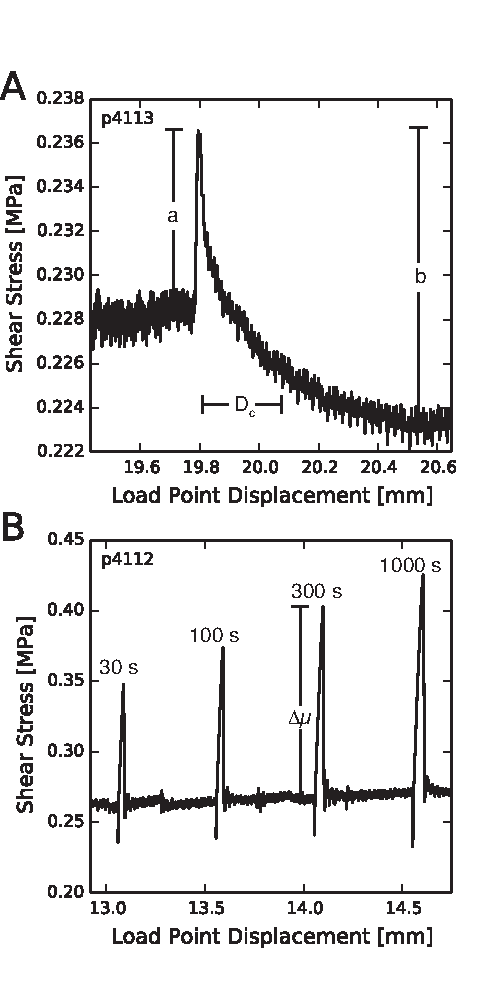
\includegraphics{chap_granular_stiffness/Fig1.pdf}
\caption{\label{fig:tests}
Experimental data showing examples of tests used to measure rate-and-state frictional parameters. (A) velocity step test in which loading velocity is changed from 150 $\mathrm{\mu}$m/s to 500 $\mathrm{\mu}$m/s. Note transient evolution of friction followed by attainment of a new steady-state. (B) results for four slide-hold-slide tests in which shearing velocity is set to zero for a period (the hold) before re-shearing, showing holds of 30, 100, 300, and 1000 seconds. Frictional healing ({}$\mu$) increases with the logarithm of hold time.}
\end{figure}

\begin{figure}
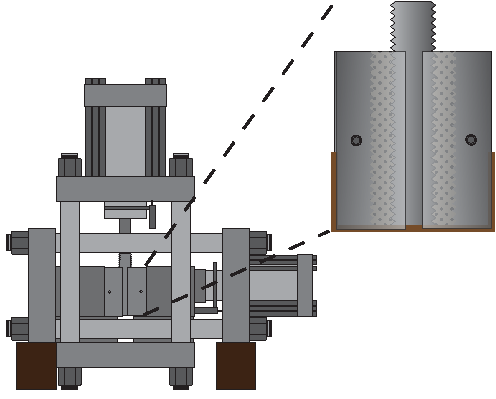
\includegraphics{chap_granular_stiffness/Fig2.pdf}
\label{fig:biax}
\caption{The biaxial press with supporting and forcing blocks in place.  Double-direct shear samples consist of three blocks: two side blocks and a center block.  Gouge layers are between the forcing blocks and confined with side-shields and a rubber membrane. (After \cite{Leeman_2014})}
\end{figure}

\begin{figure}
\begin{center}
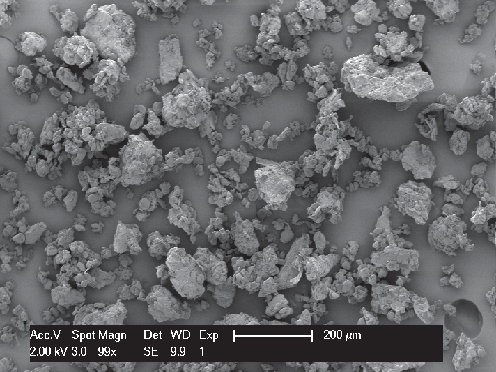
\includegraphics{chap_granular_stiffness/Fig3.pdf}
\caption{\label{fig:flour_sem}
A scanning electron micrograph of undeformed baking flour.  Grain sizes are observed to vary in the 10-200 $\mu m$ range.  The material has a platy appearance reminiscent of clay and other phyllosilicate minerals.}
\end{center}
\end{figure}


\begin{figure}
\begin{center}
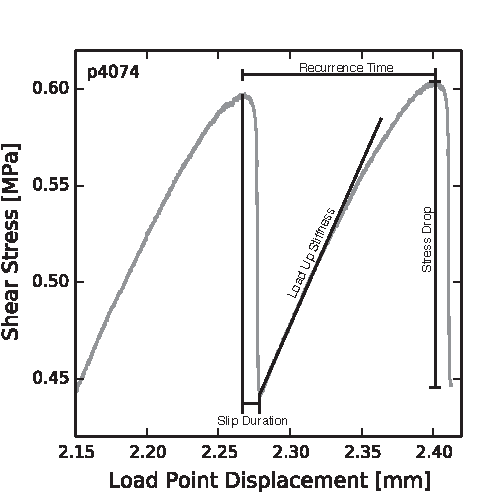
\includegraphics{chap_granular_stiffness/Fig4.pdf}
\caption{\label{fig:stickslip}
Slow-slip and stick-slip events can be characterized by their slip duration, recurrence time, stress drop, and elastic loading stiffness.  These quantities can be used to quantify the effective system stiffness and frictional properties including the rate of restrengthening (healing).    }
\end{center}
\end{figure}



\begin{figure}
\begin{center}
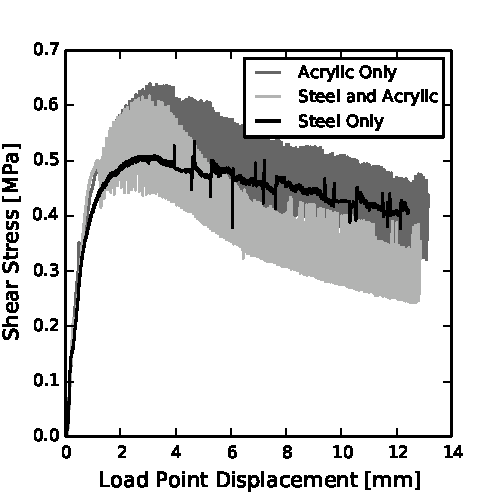
\includegraphics{chap_granular_stiffness/Fig5.pdf}
\caption{\label{fig:comp_runplots}
Data for three experiments with different forcing blocks and effective system stiffnesses.  The acrylic only and steel-acrylic experiments exhibited slow stick-slip behavior, while steel forcing blocks produced only stable sliding.}
\end{center}
\end{figure}



\begin{figure}
\begin{center}
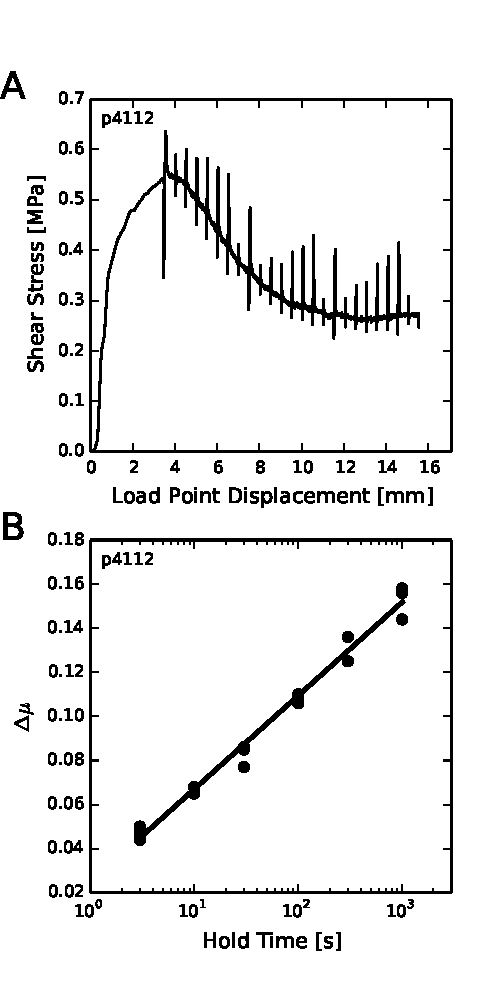
\includegraphics{chap_granular_stiffness/Fig6.pdf}
\caption{\label{fig:healing_p4112}
(A) Friction data during slide-hold-slide tests over an entire experiment with steel forcing blocks. Note initial load-up: there is a region of peak strength followed by weakening and the attainment of steady-state strength after shear of $\sim$ 10 mm.  This test included three sets of holds lasting from 3 to 1000 seconds. (B) Friction parameter $\Delta \mu$ vs. the log of hold time for the slide-hold-slide tests shown in panel A.  Healing exhibits log-linear behavior, independent of net shear displacement. }
\end{center}
\end{figure}

\begin{figure}
\begin{center}
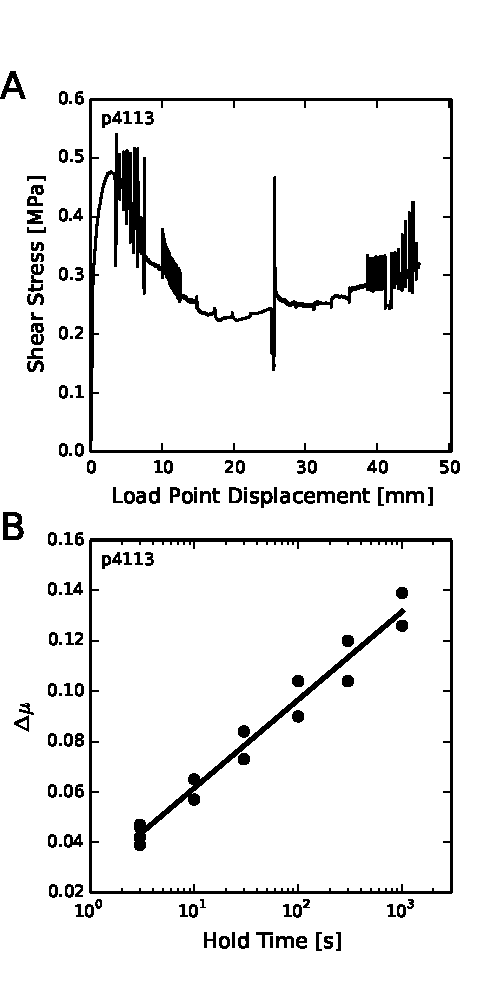
\includegraphics{chap_granular_stiffness/Fig7.pdf}
\caption{\label{fig:healing_p4113}
(A) Friction data for experiment p4113 with steel loading blocks, and (B) healing determined from slide-hold-slide tests. The sample exhibited limited stick-slip/slow-slip behavior, but only at a load point velocity of 5 $\mu m/s$.  Frictional instability appears as a wide band of noise at the scale shown, around 10 and 40 mm load point displacement. Holds ranged from 3 to 1000 seconds and velocity steps from 5 to 1500 $\mu m/s$.}
\end{center}
\end{figure}



\begin{figure}
\begin{center}
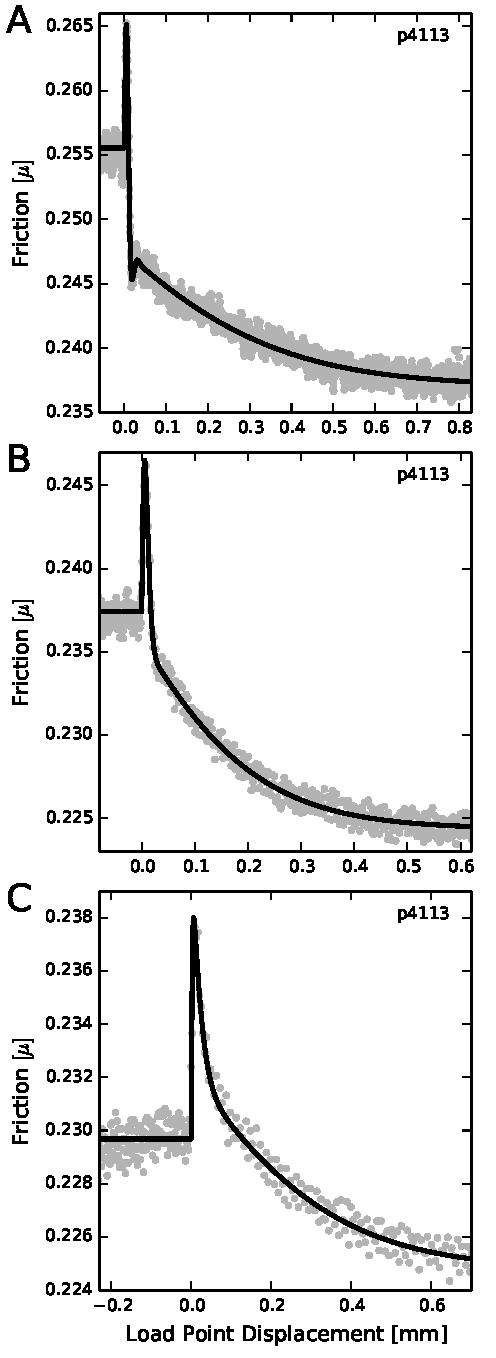
\includegraphics{chap_granular_stiffness/Fig8.pdf}
\caption{\label{fig:model_fits}
Velocity steps in an all steel forcing block configuration can only be fit by a two state variable model.  A) 15 - 50 $\mu m/s$ B) 50 - 150 $\mu m/s$ C) 150 - 500 $\mu m/s$}
\end{center}
\end{figure}


\begin{figure*}
\begin{center}
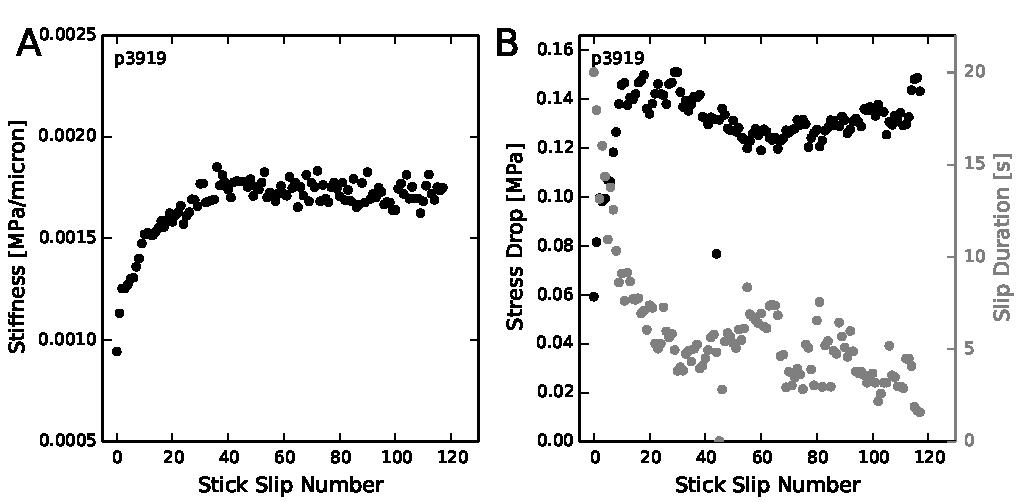
\includegraphics{chap_granular_stiffness/Fig9.pdf}
\caption{\label{fig:p3919_picks}
(A) Stiffness and (B) Stress drop and slip duration for events in experiments with all acrylic forcing blocks.  Stiffness increases on the rise to steady state by a factor of nearly two and remains remarkably constant. Stress drops rapidly increase by a factor of two over the first twenty events before reaching a steady state.  Slip duration begins at nearly twenty-five seconds, then rapidly decreases to around five seconds.}
\end{center}
\end{figure*}

\begin{figure*}
\begin{center}
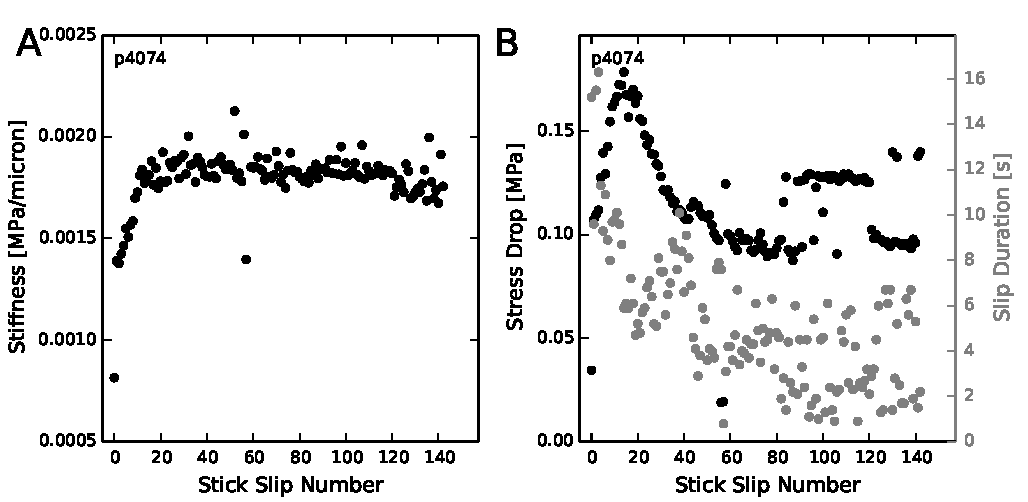
\includegraphics{chap_granular_stiffness/Fig10.pdf}
\caption{\label{fig:p4074_picks}
(A) Stiffness and (B) Stress drop and slip duration for events in the steel/acrylic forcing block system. Stiffness follows a similar trend to the all-acrylic experiment, but exhibits a smaller increase with strain. Stress drop increases rapidly, but then returns and maintains its initial level until a second family of events occurs around events 80-120.  Slip duration begins faster than for the all-acrylic blocks and stays lower with more scatter.  }
\end{center}
\end{figure*}

\begin{figure}
\begin{center}
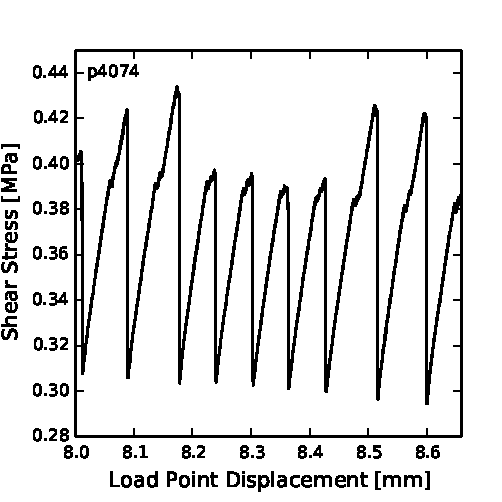
\includegraphics{chap_granular_stiffness/Fig11.pdf}
\caption{\label{fig:double_ss}
Two groups of stick-slip events are evident after sufficient shearing in the steel/acrylic system.  At the expected shear failure point there are several small failures, but the layer recovers and continues to load to a higher stress before failure.}
\end{center}
\end{figure}




\begin{figure}
\begin{center}
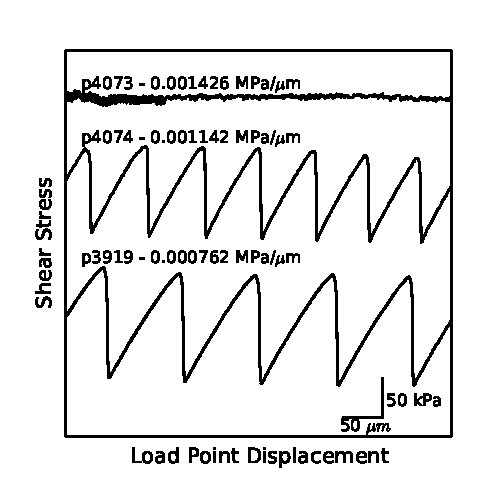
\includegraphics{chap_granular_stiffness/Fig12.pdf}
\caption{\label{fig:transition}
Response of the system with various effective stiffnesses.  The stability
boundary is crossed between the steel and steel/acrylic system.  Stiffnesses
shown are the initial load up stiffnesses of the sample.  All data are from the
same displacement range, but have been offset in shear stress for clarity. }
\end{center}
\end{figure}

\begin{table*}
\begin{center}
\begin{tabular}{cccccccc}
$V_0$ & $V$ & $a$ & $b_1$ & $D_{c_1}$ & $b_2$ & $D_{c_2}$ & $a-b$ \\
\hline
\hline
15&50&0.0120&0.0185&5.351&0.0088&207.912&-0.0154\\
50&150&0.0110&0.0125&7.448&0.0105&127.545&-0.0119\\
150&500&0.0077&0.0056&15.432&0.0061&199.407&-0.0041\\
\hline
\end{tabular}
\end{center}
\caption{Two state variable parameters obtained from friction data inversion with all steel forcing blocks (p4113).}
\label{rsf_params}
\end{table*}

\begin{table*}
\begin{tabular}{cccccc}

Experiment & Blocks & Layer Thickness (mm) & Temperature (C) & Relative Humidity (\%) & Loading Stiffness (MPa/$\mu$m) \\
\hline
\hline
p3916 & Acrylic & 7 & 23.5 & 22 & 0.000630  \\
p3918 & Acrylic & 7 & 23.1 & 22 & 0.000917  \\
p3919 & Acrylic & 7 & 24.2 & 23.9 & 0.000762  \\
p3920 & Acrylic & 7 & 24.4 & 25 & 0.000871 \\
p3917 & Steel/Acrylic & 7 & 22 & 21.9 & 0.001002  \\
p4074 & Steel/Acrylic & 8 & 23.1 & 38.8 & 0.001142 \\
p4073 & Steel & 8 & 23.4 & 28.4 & 0.001426  \\
p4112 & Steel & 8 & 24.3 & 55.5 & 0.001184  \\
p4113 & Steel & 8 & 24.3 & 56.1 & 0.001070  \\
\hline
\end{tabular}
	\caption{Load up stiffnesses during run-in for different forcing block configurations.  Note that the steel/acrylic combination is much closer to the stiffness of all steel blocks than that of all acrylic blocks.}
	\label{load_stiffness}
\end{table*}


\chapter{Laboratory observations of slow earthquakes\\ and the spectrum of tectonic fault slip modes}

\section{Abstract}
Slow earthquakes represent an important conundrum in earthquake physics. Whereas regular earthquakes are catastrophic events with rupture velocities governed by elastic wave speed, the processes that underlie slow fault slip phenomena, including recent discoveries of tremor, slow slip, and low frequency earthquakes, are less understood. Theoretical models and sparse laboratory observations have provided insights, but the physics of slow fault rupture remain enigmatic. Here we report on laboratory observations that illuminate the mechanics of slow slip phenomena.  We show that a spectrum of slow slip behaviors arise near the threshold between stable and unstable failure, and is governed by frictional dynamics via the interplay of fault frictional properties, effective normal stress, and the elastic stiffness of the surrounding material. This generalizable frictional mechanism may act in concert with other hypothesized processes that damp dynamic ruptures, and is consistent with the broad range of geologic environments where slow earthquakes are observed.

\section{Introduction}
Slow earthquakes are a mode of self-sustained fault rupture in which slip accelerates but does not reach rates sufficient to radiate high-frequency seismic energy1,2. Seismic and geodetic observations reveal that slow slip and the related phenomena of low-frequency earthquakes and non-volcanic tremor define a spectrum of slip behaviors that unfold over timescales ranging from seconds to months2-6. Slow earthquakes can be large, in some cases equivalent to M7+ earthquakes, and they may play a role in stress transfer and thus triggering of damaging regular earthquakes7.  Slow earthquakes have also been observed as precursors to regular earthquakes and thus they may provide insight into the processes of earthquake nucleation8,9.  Although geophysical observations have resolved fine details of slow earthquake slip and propagation rates of tectonic fault tremor6,8-10, the fundamental and controlling mechanics of these phenomena remain enigmatic. 
Regular earthquakes have long been understood in terms of stick-slip failure dictated by frictional and elastic properties of Earth?s crust11. Laboratory studies have provided key insights into the physics of fault failure and its dynamics, both for repeating earthquake-like stick-slip failure and for more complex slip behaviors. For example, previous works have reported a range of observations including transient slip, oscillatory sliding behavior, and dynamic rupture at sub-Raleigh and supershear propagation speeds12-18.  Transient and oscillatory behavior have been interpreted as analogs for premonitory slip prior to earthquakes or transient aseismic slip12,18,19.  
Despite their relevance to natural fault zones and slow earthquakes, detailed laboratory observations of repetitive slow slip transients are few and do not include systematic studies. These behaviors have been reported in some experimental work12,14,15, but have been interpreted and modeled in the context of specific fault rheologies, using so-called ?designer? friction laws. In one form of these laws, slow stick-slip is produced by an increase in frictional resistance with slip velocity, such that instability is quenched during acceleration14,15,19.  Other explanations for slow earthquakes have focused on processes that may arrest slip acceleration during earthquake nucleation, including dilatancy hardening20,21, transitional frictional behavior as a function of slip22 or slip rate, and fault zone heterogeneity.  Some numerical simulations successfully predict complex slip behavior, including oscillatory behavior and the emergence of periodic slow slip20,23. Two dimensional numerical models also show promise in reproducing natural events, with fewer free parameters than multiple state variable models26. 
To date, the origin of slow earthquakes has been explored largely via seismic or geodetic data or through numerical experiments with only sparse, isolated laboratory observations to probe the underlying mechanics.  Although theoretical models can explain the emergence of slow-slip transients under certain conditions or for specific frictional rheologies20,21,23, a fundamental mechanical explanation for these events remains elusive. Yet, slow modes of fault rupture are observed in a variety of tectonic and geologic settings, and with a wide range of durations, raising the question as to whether they arise from a universal mechanism6,24. 
Although many fault zones are rich in phyllosilicate minerals, which have been shown to exhibit both rate-weakening and rate-strengthening behavior under conditions comparable to those expected in situ in the seismogenic crust25-27, we focus on quartz gouge to investigate the systematics of frictional failure, because it is a well-studied material that is common in natural faults, and is thought to play a key role in controlling their slip behavior27,28. Quartz gouge also exhibits frictional properties that enable us to probe the stability boundary using geophysically-relevant values of normal stress and sliding rates. This allows a detailed investigation of the frictional dynamics of slow slip, which provides a robust and generalized framework to apply to tectonic fault zones. 
Here we describe laboratory experiments that reproduce the full spectrum of fault slip behaviors under geophysically relevant conditions of normal stress and fault composition, and which illuminate their underlying physics. Our experiments are designed to explore the full range of slip stability, as described by the stability parameter ?=k/kc, from ?>1 (inherently stable slip) to dynamic stick-slip (?<<1). Consistent with previous works14,18,23 near the stability boundary, ??1, we observe complex slip patterns that precede slow slip. We document a systematic and robust relationship between departure from the stability threshold, slip velocity, and duration of repetitive failure events. Our experimental results, to the best of our knowledge, are the first complete and systematic study to investigate the full spectrum of slip behaviors from slow to fast events, as observed for tectonic faults. 

\section{Results}
\subsection{Mechanical Behavior}
In our experiments, gouge layers initially exhibited stable sliding, followed by the emergence of repeating slow stick-slip events (Figure 1, 2A). The slow slip events arose gradually, over an interval of up to 1.5 mm, and then increased in amplitude over as few as 10-20 slip events before reaching a mechanical steady-state, characterized by relatively uniform recurrence intervals and friction drops, up to the maximum imposed displacements of ? 50 mm.  For our layers, which were 3-mm thick prior to shear, this corresponds to shear strains of 30-50.  Each slow-slip event began with a gradual acceleration and culminated in a slip event and stress drop (Figure 1). 
\subsection{Stick-Slip Events}
Our experimental results are consistent with theory, numerical experimentation,20,23and with existing lab data for stick-slip11. We document a spectrum of stick-slip behaviors in experiments conducted over a range of normal stresses (Figure 2A). At low normal stress (6 MPa) and close to the stability transition described by Equation (1), slip events have systematically longer duration and smaller stress drops than their higher normal stress counterparts (Figure 2C). Details of the friction records for slow events show that slip begins gradually, well before the peak strength is reached, and then accelerates during the stress drop (Figure 2B).  The maximum slip velocities for slow-slip events are in the range of 50-100 �m s-1, and slip speed increases systematically with increasing normal stresses, which leads to increasingly unstable behavior (Equation 1).  For the lowest values of normal stress that produced repeating transient slip events, we measured peak slip velocities of only a few 10?s of �m s-1, on the order of the driving velocity. For a normal stress of 14 MPa, we observed audible fast stick-slip events with slip velocities > 2 mm s-1. 

\section{Discussion}
The short duration, audible high slip velocity events are manifestations of dynamic instability and represent laboratory analogs of regular, fast earthquakes11.  Likewise, we posit that the observed spectrum of slow to fast stick-slip events in our experiments are representative of the spectrum of slip behaviors observed on tectonic faults, including repeating slow slip events and low frequency earthquakes4,6. Near the stability transition, we also document complex and chaotic behaviors including period doubling and transient variations in stick-slip amplitude with long period modulation (Figure 2A), consistent with theoretical predictions 23.
To investigate the mechanics of slow stick-slip events, we carefully measured both the elastic loading stiffness k and the critical stiffness kc in each of our experiments.  We measured k directly from the loading curves of stick-slip events and from unload/reload cycles (Supplementary Figure 1).  Stiffness increases with shear displacement up to 15 mm, and then reaches an approximately constant value (Figure 3; Supplementary Figure 1). The increase in stiffness with shearing is consistent with shear-enhanced compaction and granular comminution during the first few mm of slip29. As noted above, we measure kc directly from the parameters in Equation 1 using velocity step experiments (Figure 3A, Supplementary Figure 2), and also empirically using the value of k? at the observed transition between unstable and stable slip (black line, Figure 3B). The empirically defined threshold stiffness increases with displacement and reaches a steady value of ? 7x10-4 �m-1 at a displacement of ~16 mm, equivalent to a shear strain of ~5-6 (Figure 3B). Direct measurements of kc yield similar values (6-7x10-4 �m-1; Supplementary Figure 2), and also show that kc increases dramatically within the first ~10 mm of shear displacement. This is due to the combined effects of increasingly velocity weakening friction (Figure 3A) and decreasing critical slip distance Dc with shear strain (Supplementary Figure 2). The evolution of (b-a) is consistent with inferred shear localization and with the observation that unstable slip emerges after a finite shear strain (Figure 1). The shear displacement needed for the emergence of slow-slip decreases with increasing ?n? (Figure 2A), consistent with enhancement of shear localization and fabric development at higher ?n?.  
Taken together, our direct (Figure 3A, Supplementary Figure 2) and independent (Figure 3B) measurements of kc? and k? (Supplementary Figures 1, 2) show that stick-slip event velocity and duration vary systematically as a function of distance from the stability threshold. The slowest events occur for $\kappa$ ? 1, with progressively faster events for lower values of $\kappa$ (Figure 3D, 3E). The peak slip velocity and stick-slip duration for all events, measured after reaching a steady-state (Figure 3C, shaded area), define a complete spectrum of slip behaviors between stable sliding and fast stick-slip (Figure 3D, 3E). For $\kappa$ < 0.7, slip velocities of several mm s-1 were associated with audible failure events (Figure 3D). For values of $\kappa$approaching 1, the duration of slow-slip is on the order of seconds (not producing any audible emissions in the range of human hearing), with lower peak slip velocities (Figure 3D, 3E). The amplitude of the stick-slip events is systematically lower for the slow events (Figure 2), consistent with seismic and geodetic observations for tectonic faults4,6,30.
Our data show that the full spectrum of stick-slip behaviors can occur over a relatively narrow range of conditions near the stability phase boundary, and further, that the mode ? and slip velocity ? of unstable sliding vary predictably as a function of departure from this threshold. Although the 1-D spring-slider model is simplified relative to the geometry and rheology of natural fault systems, the predicted stability regimes are remarkably consistent with our laboratory experimental data. It is also consistent with theoretical models that incorporate more complex 2-D fault geometries and elastic interactions20, suggesting that to first order, the mechanics and dynamics of these systems are captured by this relatively simple and elegant model15,18,23,29,31. 
In total, our results illuminate the key ingredients required for slow earthquakes. Relative to areas where regular earthquakes occur, kc must remain sufficiently small that it does not greatly exceed the local fault stiffness k. This can occur for specific frictional properties ? small (b-a) or large Dc ? as may be the case at the upper and lower edges of the seismogenic zone or in areas of complicated fault zone architecture20. This condition would also be favored by low effective normal stress, as has been suggested in a wide range of settings8,9,31-34. Additionally, we suggest that the mode of fault slip should evolve as tectonic faults accumulate shear strain, or through the earthquake cycle, due to progressive changes in fault stiffness and frictional constitutive properties32,34. Finally, because fault stiffness is proportional to the ratio of shear modulus to rupture nucleation patch size, we expect that regions of large, coherent creep slip, which effectively reduce k, would favor nucleation of slow earthquakes.  
Our results support previous hypotheses about the role of transitional frictional behavior in driving complex fault slip behaviors20,23,31-33. It is likely that transitional frictional behavior may act in concert with additional processes acting locally within a fault zone to produce the observed spectrum of slip behaviors. A wide range of key natural factors, such as compliant and evolving damage zones, low effective normal stress associated with elevated pore fluid pressure and, fault evolution are all captured by the stability parameter $\kappa$=k/kc. Ultimately, our results suggest that slow earthquakes and transient fault slip behaviors arise from the same governing frictional dynamics as normal earthquakes, and provide a unified view of the spectrum of tectonic fault slip behaviors. 

\section{Methods}
\subsection{Experimental Apparatus}
Experiments were performed in a servo-controlled biaxial shearing apparatus using the double direct shear configuration (Figure 1). Displacements on the normal and shearing axes were measured by Direct Current Displacement Transducers (DCDTs), referenced at the load frame and ram nose. The displacement of the shearing block was measured with DCDTs referenced at the end-platen and the top and bottom of the shearing block (Figure 1). Loads applied to the sample were measured with strain gauge load cells. All transducers are calibrated with instruments and methods traceable to NIST. 
Sample Preparation
Samples were prepared using steel or titanium side blocks and steel or acrylic (PMMA) central shearing blocks (Supplementary Table 1). The forcing blocks were grooved 0.8 mm deep at 1 mm spacing to eliminate shear at the boundary. We used Min-U-Sil 40 powdered silica (U.S. Silica Co.) to simulate granular fault gouge. The product is 99.5\% SiO2, with traces of metal oxides, and has a median grain diameter of 10.5 ?m. Samples were constructed as 3-mm thick layers, and with 10 cm x 10 cm frictional contact area. Layers were prepared and sheared under 100\% relative humidity at room temperature. 

\subsection{Testing Procedure}
After samples were placed in the testing machine, a constant normal stress was applied and maintained constant using force-feedback servo control. Samples were allowed to compact and accommodate grain rearrangement before shearing began. Shear was induced by imposing a displacement rate on the central forcing block (Figure 1), using a feedback servo control. The displacement rate was maintained constant at 10 ?m s-1 for the majority of our experiments (Supplementary Table 1), and velocity step tests were used to determine the friction rate parameters (a-b) and Dc.
We used a range of shear loading stiffnesses k given by the summation, in series, of the apparatus stiffness, the stiffness of the loading blocks, and the stiffness of the layers of fault gouge. The effective loading stiffness of the testing machine k?=k/?n? was altered by using a compliant central forcing block (PMMA) and by changing the applied normal stresses (Figure 2A).  We measured k in experiments using a least-squares linear fit to friction vs. shear displacement for the interval ? = 0.3 ? 0.4 and from the elastic loading portion of stick-slip events (Supplementary Figure 1). Rate-and-state friction parameters were determined (Supplementary Figure 2) using an iterative singular value decomposition technique. 
Frictional Stability
In the context of frictional stability, the criterion for unstable stick-slip in a simplified 1-D system is defined by the interaction between loading system stiffness k and a rheologic critical stiffness of the fault, kc: 
	k < kc =  ?n? (b-a)/Dc	(1)
where (b-a) is the friction rate parameter and Dc is the critical slip distance29. Negative rate parameters, (b-a) < 0, indicate velocity-strengthening behavior, which is inherently stable. Positive values of (b-a) indicate velocity-weakening friction and are a prerequisite for instability and earthquake nucleation. Within the velocity weakening regime, if the condition in Equation (1) is satisfied (i.e. stiffness of the loading system, k, is less than the critical stiffness; k < kc), instability occurs because the fault weakening rate, kc, exceeds the rate of elastic unloading, leading to a force imbalance. For stiffer systems (i.e. k > kc), in which elastic unloading outpaces frictional weakening, sliding is stable. For convenience, we normalize the stiffness and critical stiffness by the normal stress, appending a prime symbol to denote this; k? = k/?n? and kc? = kc/?n?
We selected values of k and normal stress for our experiments to span the stability boundary for our fault gouge.  To achieve this, we made careful measurements of the evolution of k and kc with shear strain (Supplementary Figure 1). For a given set of frictional properties, defined by (b-a) and Dc, the ratio k/?n? defines an effective system stiffness, k? [�m-1], that governs sliding stability. In our experiments, the testing machine, sample assembly, and gouge layer together determine the system stiffness. We varied k using different forcing block materials (Supplementary Table 1) and k? via the normal stress.  

% Figure %
\begin{figure}
	\centering
		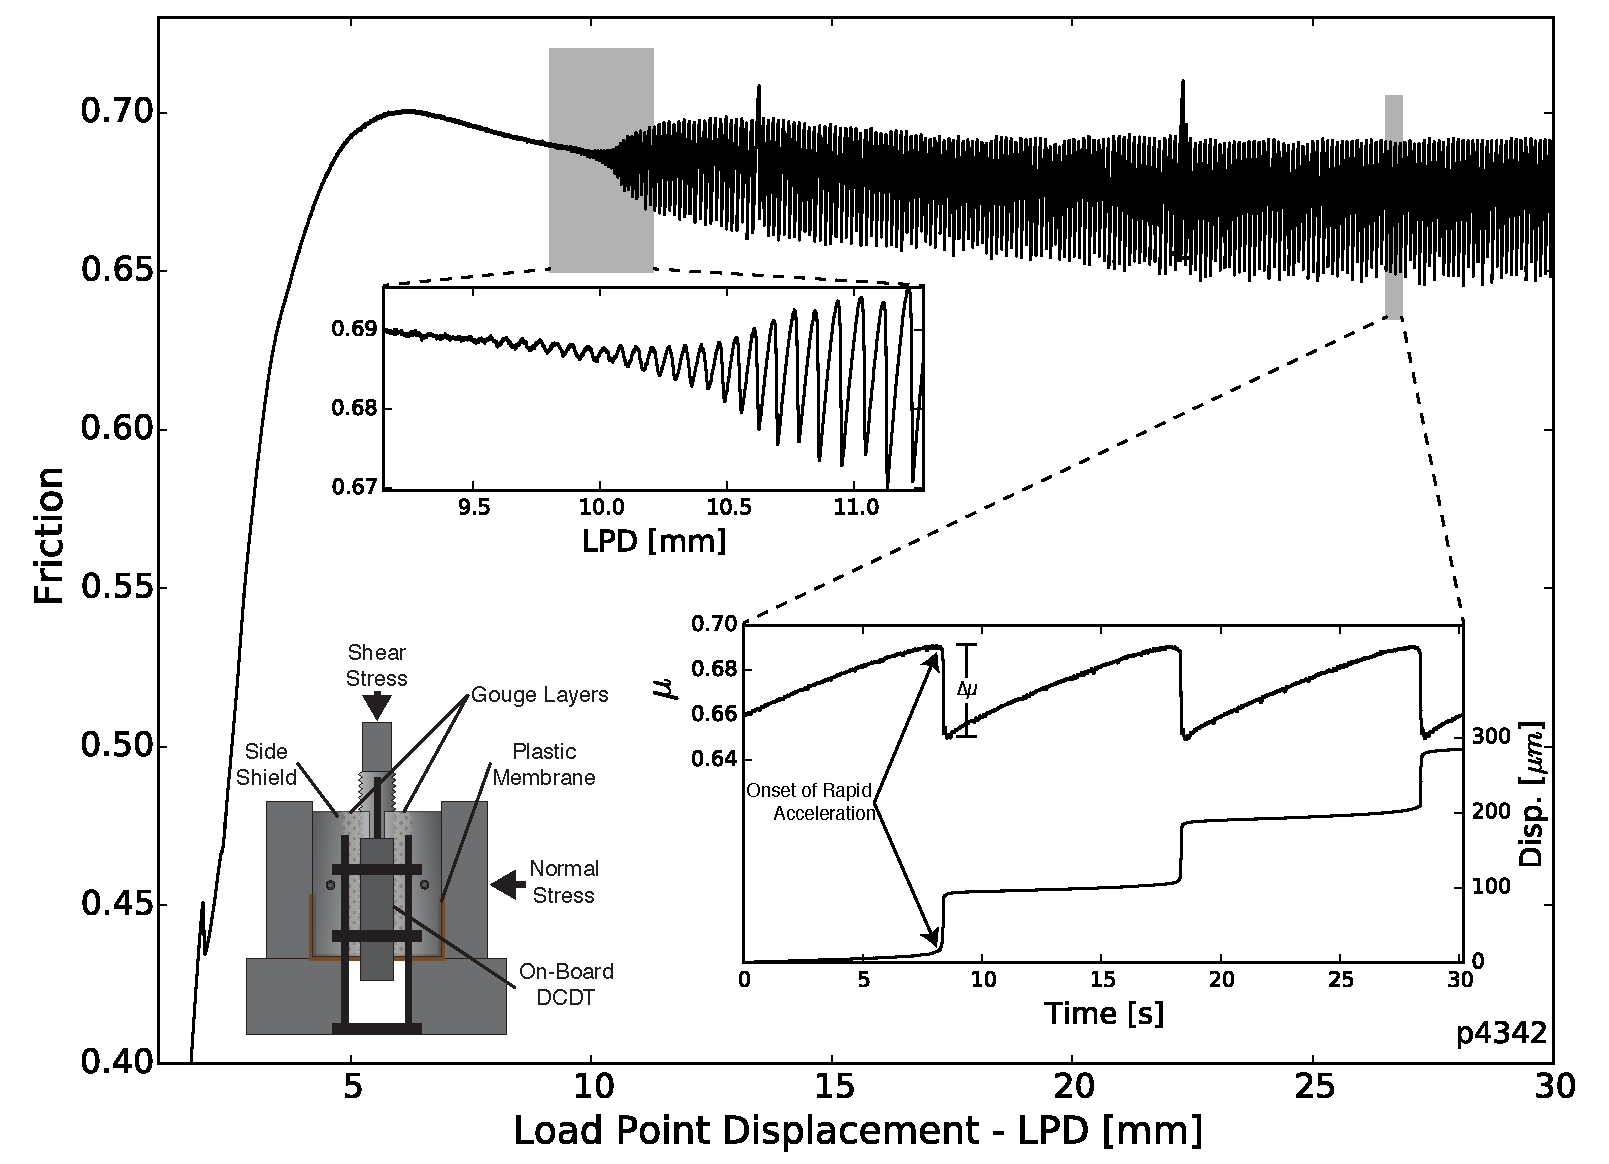
\includegraphics[scale=1.0]{chap_lab_slow_eq/Figure_1.pdf}
   	\caption{Experimental run plot. Friction data for one experiment (p4342) at a normal stress of 12 MPa and shearing rate of 10 �m s-1. The upper inset shows spontaneous emergence of unstable slow slip. Stick-slip amplitude increases gradually over a few mm before reaching steady-state.  The lower right inset shows details of fault slip events, note the gradual acceleration at the start of each failure event. The lower left inset shows the double direct shear configuration and locations of displacement transducers. Spikes at 13 mm and 22 mm displacement are due to brief pauses in shearing to reset displacement transducers.}
  	\label{}
\end{figure}
% End Figure %

% Figure %
\begin{figure}
	\centering
		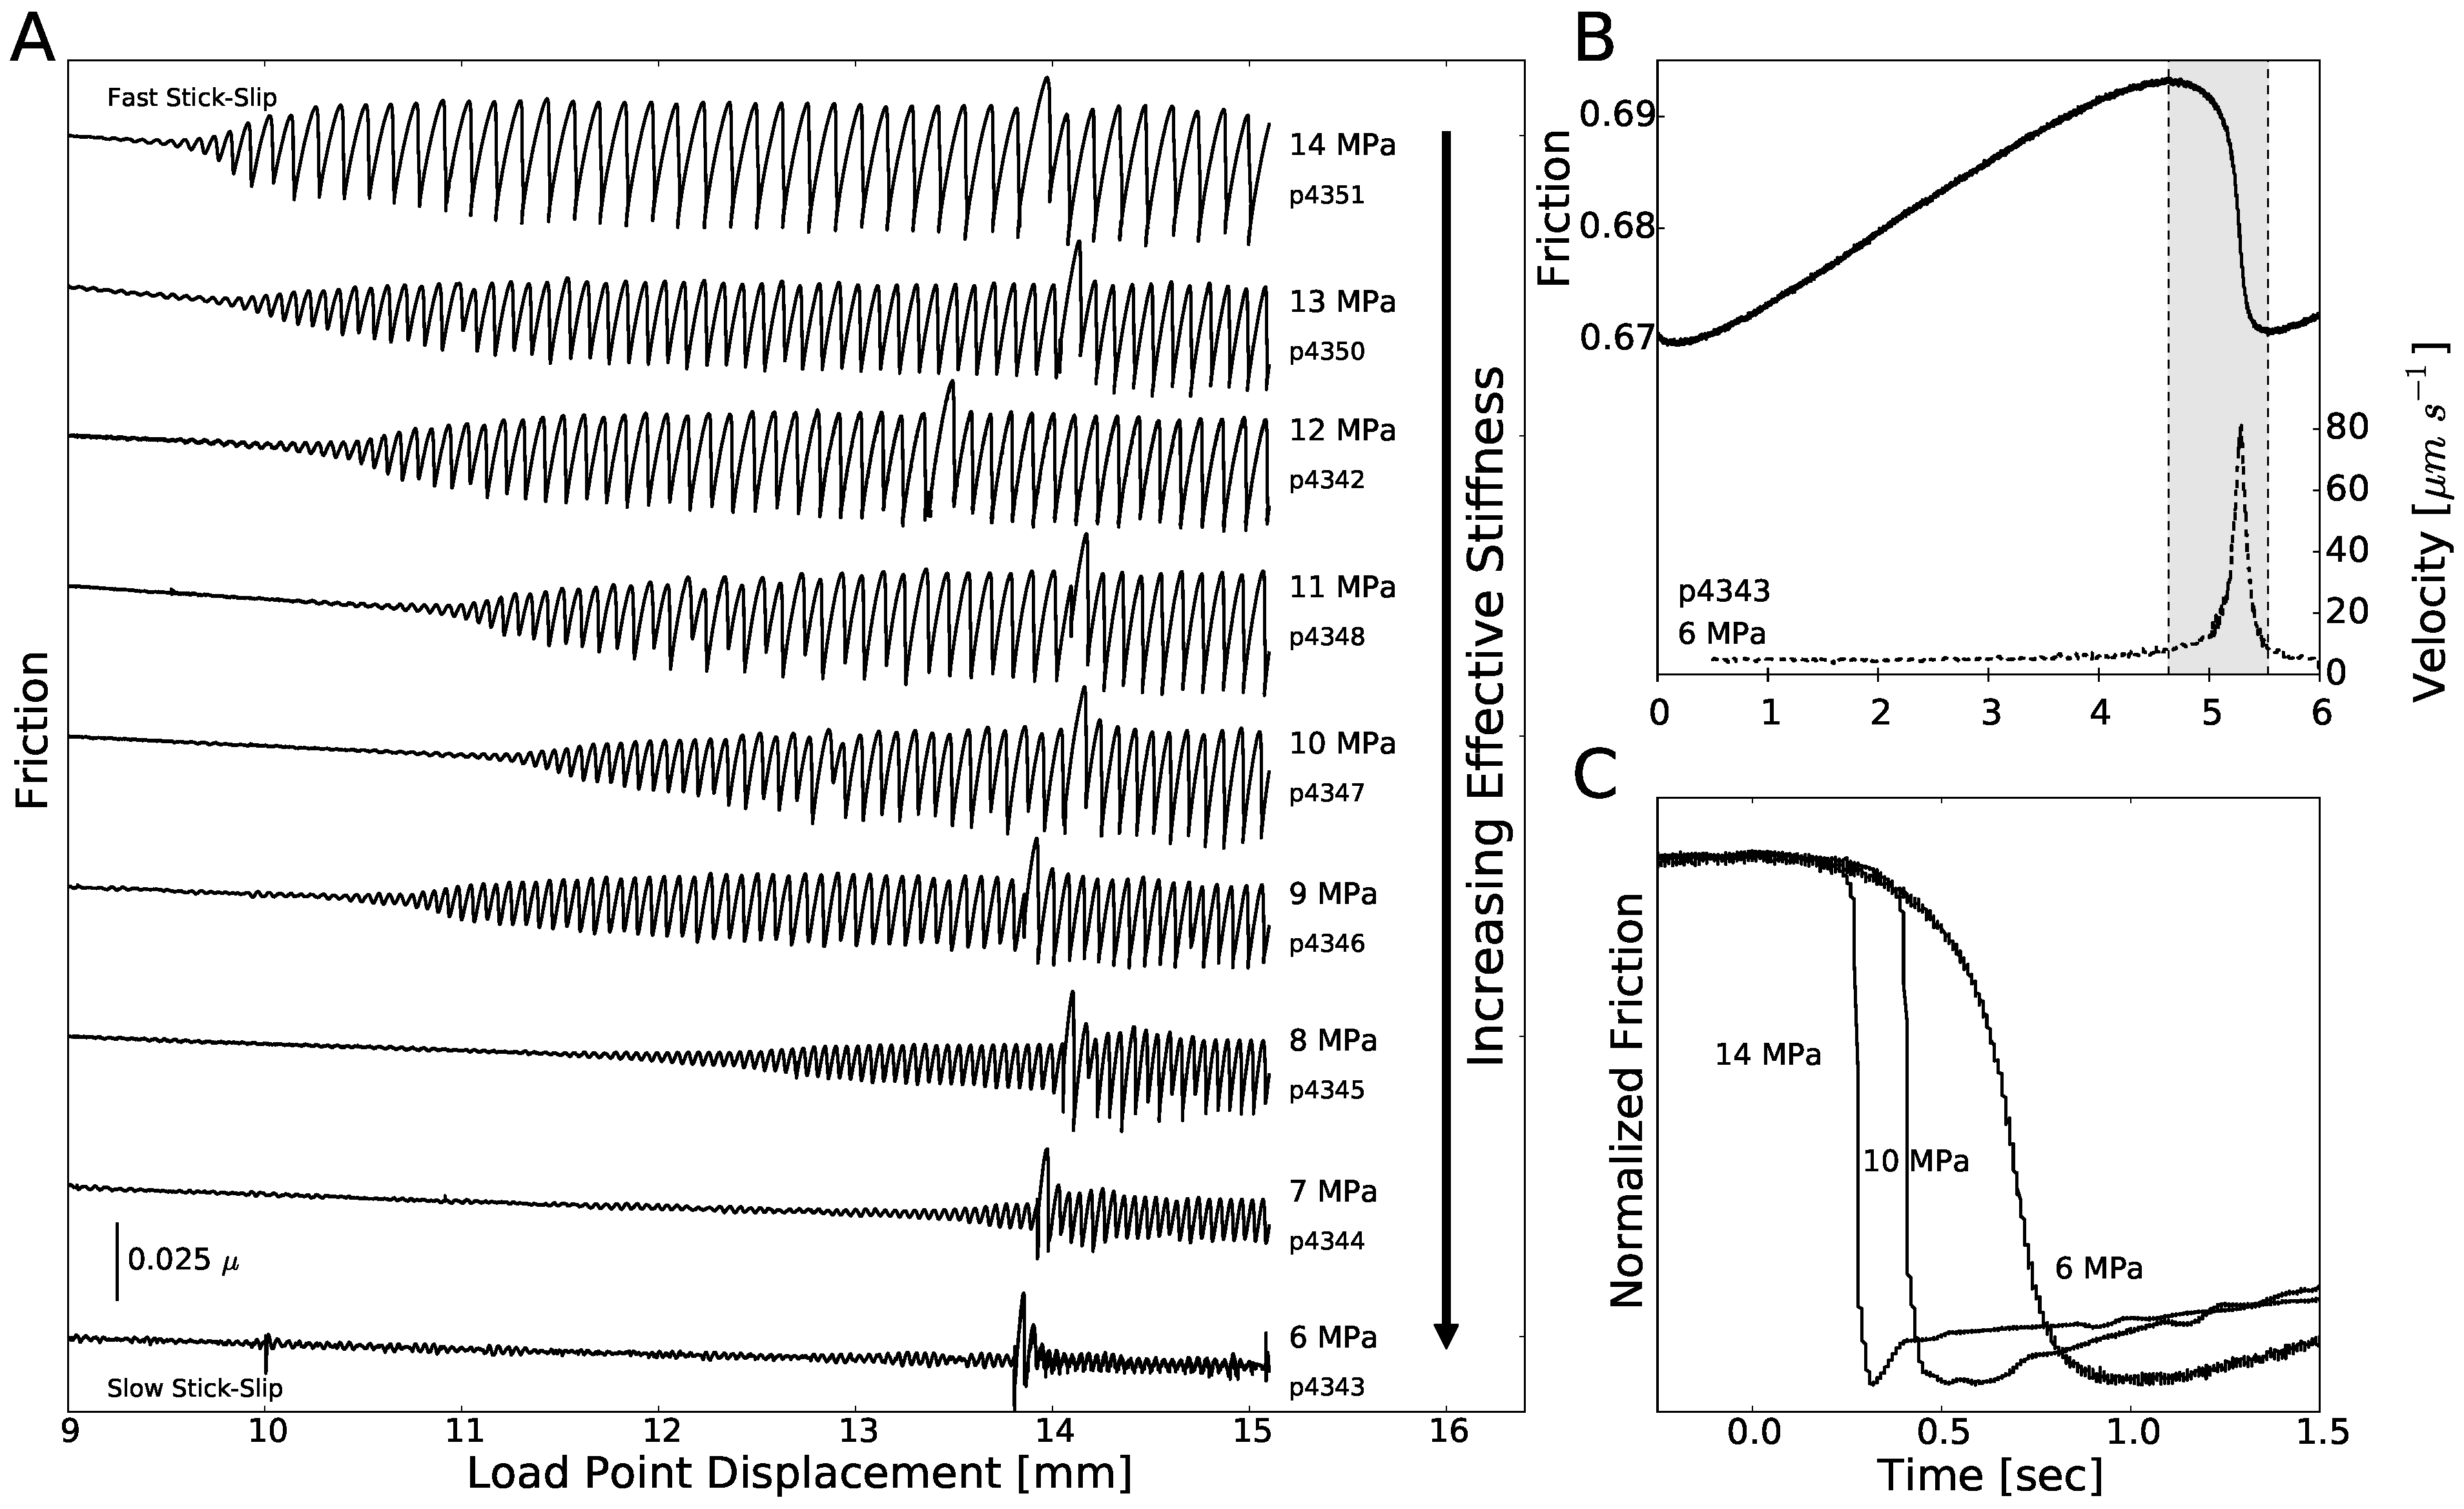
\includegraphics[scale=1.0]{chap_lab_slow_eq/Figure_2.pdf}
   	\caption{Spectrum of Fault Slip Behavior. A) Friction data for experiments (p43XX run numbers) at different effective shear loading stiffness k?=k/?n?. Friction data are offset vertically for clarity. The emergence of slow stick-slip occurs at lower shear displacement, and stick-slip amplitude increases, for higher normal stress experiments. The spikes in friction at 13-15 mm are due to frictional aging caused by brief pauses in shearing to reset displacement transducers. B) Details of friction (solid line) and velocity (dashed) during a stick-slip event with a peak slip velocity of ? 80 �m s-1, only a few times that of the background loading velocity of 10 �m s-1. C) Stick-slip events have systematically longer duration at lower normal stresses. Slip accelerates more slowly and event durations are correspondingly longer than at higher normal stress.}
  	\label{}
\end{figure}
% End Figure %

% Figure %
\begin{figure}
	\centering
		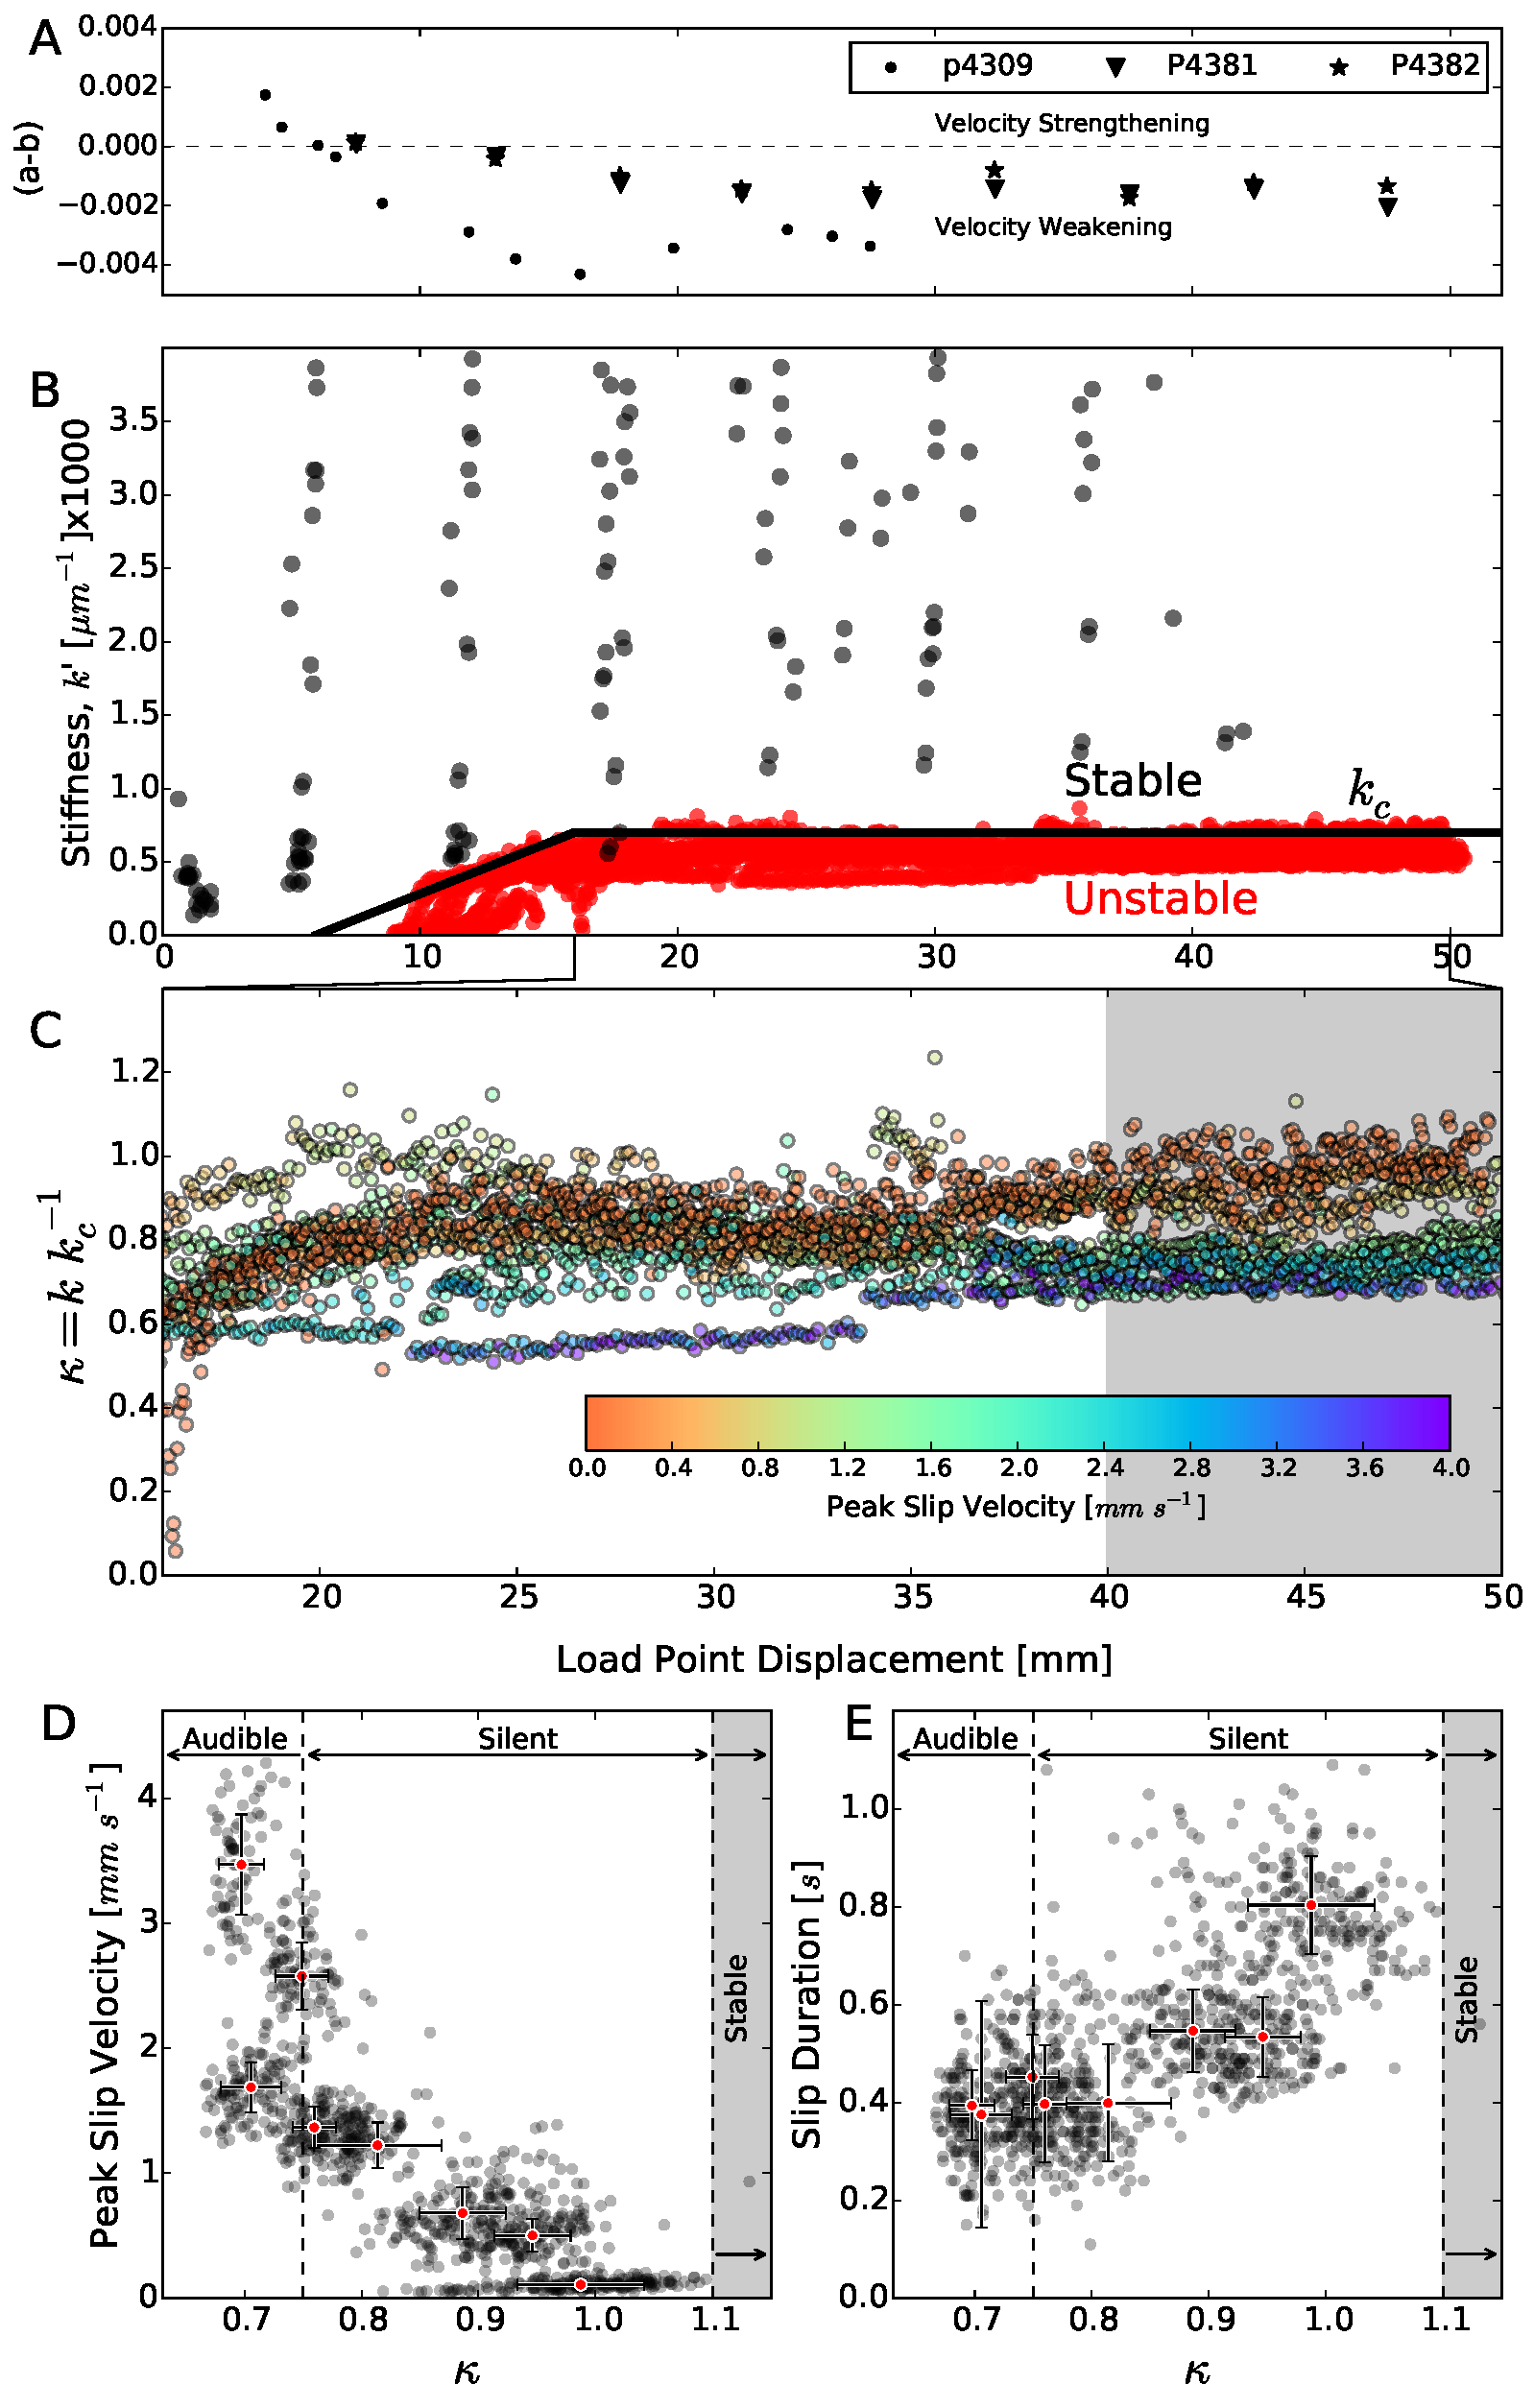
\includegraphics[scale=1.0]{chap_lab_slow_eq/Figure_3.pdf}
   	\caption{Stick slip event properties. A) The friction rate parameter (b-a) transitions from velocity strengthening 
to velocity weakening at ~5-7 mm displacement.  B) Data from 29 experiments showing effective friction stiffness k?= k/?n? as a function of shear displacement for stable sliding (black dots) and stick-slip events (red dots). The heavy black line defines the evolution of kc? based on the distinction between stable sliding and stick-slip. C) Data for unstable slip events shown in B are color coded by peak slip velocity and shown as a function of shear displacement. Stick-slip is slowest for ?  ~ 1. The 40-50 mm interval marked by the gray box denotes data used to compile stick-slip properties. D) Stick-slip event velocity and E) duration as a function of normalized critical stiffness ? = k/kc.  Black dots show data from events in the displacement interval 40-50 mm for 8 experiments; red dots show mean values �1 standard deviation for each experiment.
}
  	\label{}
\end{figure}
% End Figure %

% Figure %
\begin{figure}
	\centering
		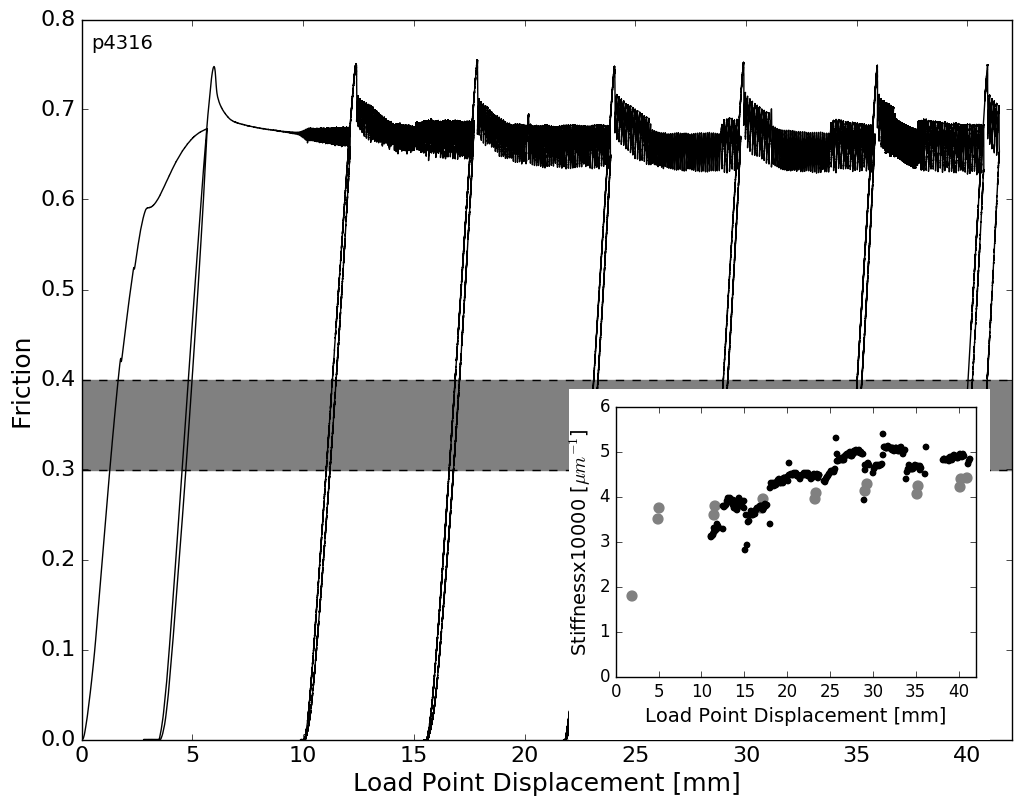
\includegraphics[scale=1.0]{chap_lab_slow_eq/Figure_S1.png}
   	\caption{Stiffness during an experiment. Friction data for one complete experiment (run p4316) with shear load-unload cycles. Slow slip events emerge spontaneously at a displacement of ~8.5 mm. (Inset) Stiffness measured from unload-reload cycles in the range �=0.3-0.4 (large grey circles) and from the slope of the elastic loading segments of individual stick-slip events (small black circles). Both measurements indicate an initial increase in stiffness, caused by shear enhanced compaction. In this experiment we explored multiple shearing rates during slow slip (e.g., for events in the range 27-29 mm and 31-33 mm), which had a clear effect on stick-slip amplitude and stiffness.}
  	\label{}
\end{figure}
% End Figure %

% Figure %
\begin{figure}
	\centering
		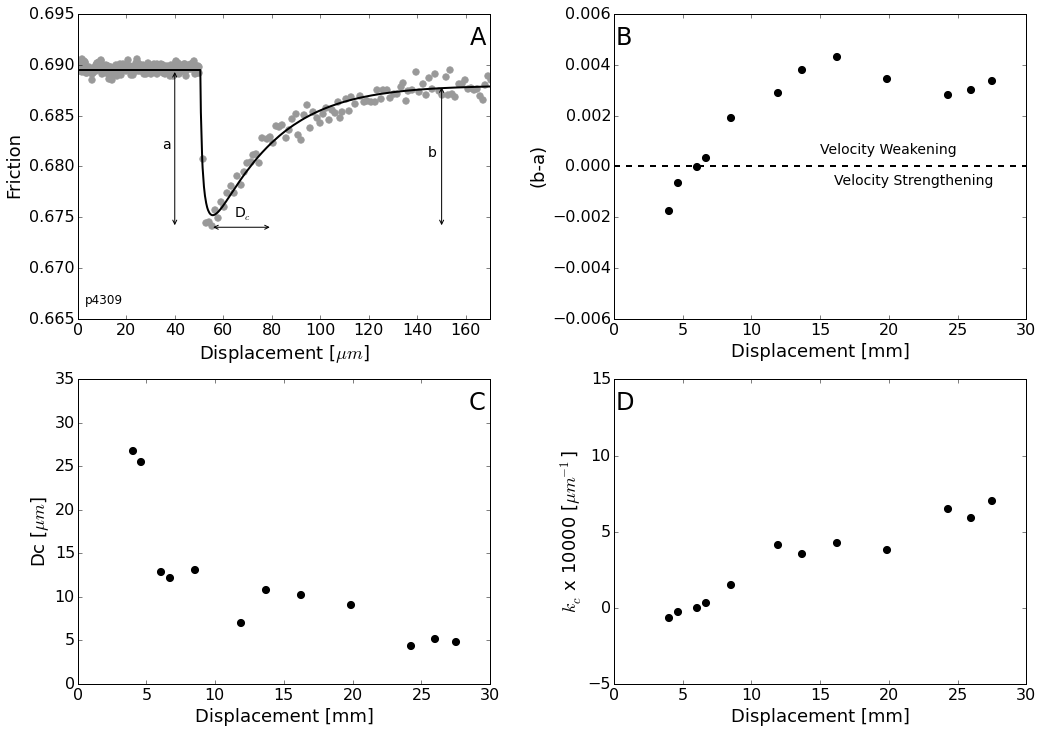
\includegraphics[scale=1.0]{chap_lab_slow_eq/Figure_S2.png}
   	\caption{Rate and State Parameters. Data and modeling procedure for obtaining rate-and-state friction parameters and their variation with shear displacement. A) Data from experiment p4309 (grey data points) and model (solid line) for a velocity step test from 10 to 1 �m s-1, with illustration of the friction direct effect a, evolution effect b, and critical slip distance Dc. B) Evolution of (b-a) with shear displacement (see also Figure 3A). Note the transition from rate strengthening to rate weakening at ~8 mm displacement, after which a steady-state behavior is reached. C) The critical slip distance decreases with shear displacement as frictional steady-state is reached. D) Evolution of the critical stiffness (kc) with slip.}
  	\label{}
\end{figure}
% End Figure %

\begin{table*}
    \begin{tabular}{ |c|c|c|c|c|c| }
    \hline
    Experiment & Blocks & Normal Stress [MPa] & Humidity [\%] & Comments & Unload/Reload Cycles\\
    \hline
    p4224 & Ti/Acrylic & 5 & 16 & Stable - Vel. Steps & N\\
    \hline
    p4228 & Steel& 4 & 100 & Stable - Slide Hold & N\\
    \hline
    p4229 & Ti/Acrylic & 4 & 100 & Failed & N\\
    \hline
    p4248 & Ti/Acrylic & 4 & 100 & Stable - Vel. Steps & N\\
    \hline
    p4249 & Ti/Acrylic & 4 & 100 & Stable - Vel. Steps & N\\
    \hline
    p4267 & Ti/Acrylic & 2 & 100 & Stable - Vel. Steps & Y\\
    \hline
    p4268 & Ti/Acrylic & 8 & 100 & Slow-Slip & Y\\
    \hline
    p4269 & Steel & 4 & 100 & Stable - Vel. Steps & Y\\
    \hline
    p4270 & Steel & 2 & 100 & Stable - Vel. Steps & Y\\
    \hline
    p4271 & Ti/Acrylic & 2 & 100 & Stable - Vel. Steps & Y\\
    \hline
    p4272 & Ti/Acrylic & 8 & 100 & Slow-Slip & Y\\
    \hline
    p4273 & Steel & 8 & 100 & Stable - Vel. Steps & Y\\
    \hline
    p4309 & Steel & 8 & 100 & Stable - Vel. Steps & Y\\
    \hline
    p4310 & Ti/Acrylic & 8 & 100 & Slow-Slip & Y\\
    \hline
    p4311 & Ti/Acrylic & 8 & 100 & Slow-Slip & Y\\
    \hline
    p4312 & Steel/Acrylic & 8 & 100 & Slow-Slip & Y\\
    \hline
    p4313 & Ti/Acrylic & 8 & 100 & Slow-Slip & Y\\
    \hline
    p4314 & Steel & 12 & 100 & Stable - Vel. Steps & Y\\
    \hline
    p4316 & Ti/Acrylic & 12 & 100 & Stick-Slip & Y\\
    \hline
    p4317 & Steel/Acrylic & 12 & 100 & Stick-Slip & Y\\
    \hline
    p4327 & Steel & 6 & 100 & Stable - Vel. Steps & Y\\
    \hline
    p4328 & Ti/Acrylic & 6 & 100 & Slow-Slip & Y\\
    \hline
    p4329 & Ti/Acrylic & 6 & 100 & Slow-Slip & Y\\
    \hline
    p4330 & Steel & 6 & 100 & Stable - Vel. Steps & Y\\
    \hline
    p4338 & Ti/Acrylic & 4 & 100 & Stable - Vel. Steps & Y\\
    \hline
    p4339 & Steel & 4 & 100 & Stable - Vel. Steps & Y\\
    \hline
    p4340 & Ti/Acrylic & 8 & 100 & Slow-Slip & Y\\
    \hline
    p4341 & Steel & 12 & 100 & Stable - Vel. Steps & Y\\
    \hline
    p4342 & Ti/Acrylic & 12 & 100 & Slow/Fast Slip & N\\
    \hline
    p4343 & Steel/Acrylic & 6 & 100 & Slow-Slip & N\\
    \hline
    p4344 & Ti/Acrylic & 7 & 100 & Slow-Slip & N\\
    \hline
    p4345 & Steel/Acrylic & 8 & 100 & Slow-Slip & N\\
    \hline
    p4346 & Ti/Acrylic & 9 & 100 & Slow-Slip & N\\
    \hline
    p4347 & Steel/Acrylic & 10 & 100 & Slow/Fast Slip & N\\
    \hline
    p4348 & Ti/Acrylic & 11 & 100 & Slow/Fast Slip & N\\
    \hline
    p4350 & Steel/Acrylic & 13 & 100 & Slow/Fast Slip & N\\
    \hline
    p4351 & Ti/Acrylic & 14 & 100 & Slow/Fast Slip & N\\
    \hline
    p4381 & Steel & 4 & 100 & Stable - Vel. Steps & N\\
    \hline
    p4382 & Ti & 4 & 100 & Stable - Vel. Steps & N\\
    \hline
    \end{tabular}
\end{table*}

\chapter{Characterization of Laboratory Slow Earthquakes}

\section{Abstract}
This chapter is currently being completed.
\chapter{Mechanical and hydrologic properties of Whillans ice \\stream till: Implications for basal strength \\and stick-slip failure}

\section{Abstract}
Ice streams transport large volumes of inland ice to the ocean and play a key role in the mass balance of the Antarctic ice sheet. The rate and style of ice stream basal slip are governed, in part, by the underlying till whose physical properties are poorly constrained. To address this problem, we conducted a suite of laboratory measurements to document the permeability, stiffness, consolidation behavior, and compressional wave speeds of Whillans Ice Stream till samples. We investigated the effects of stepped and cyclic loading on the evolution of the till. Initial permeabilities were 3.8-4.9�10-17 m2 (porosities 28.1-31.8\%), which decreased to 2.0�10-19 m2 (20.4\%) at 10 MPa effective stress. P-wave velocities span from 2.26-3 km/s over this effective stress range, and are well described by an effective medium model. The laboratory measurements were used to parameterize a 1-D numerical model to predict the till?s response to stress perturbations. Perturbations corresponding to tidal periods produce a drained and strengthened layer tens of cm thick. For perturbations over timescales of weeks to months, as expected for till motion over basement features, the drained zone is a few meters thick. This strong layer can become brittle upon unloading, and may facilitate observed stick-slip motion. Extrapolation of our effective medium model suggests low basal effective stresses, on the order of a few tens of kPa, are needed to produce seismic velocities observed in the field (Vp ~1750 m/s; Vs ~160 m/s), and provides an approach to quantify and monitor in situ conditions.

\section{Introduction}
Ice streams are regions of fast-moving grounded ice shearing past slower-moving regions of ice.  In Antarctica, ice streams discharge over 90\% of the interior accumulation over only ~13\% of the coastline, making them critical to the ice sheet mass balance [Morgan et al., 1982]. Motion of ice streams is complex, as the flow can migrate, stagnate, or even occur in a stick-slip fashion, inducing seismicity [Anandakrishnan et al., 2003; Wiens et al., 2008; Walter et al., 2011]. Many models have attempted to explain the nature of ice stream movement, mostly invoking high basal water pressures, often coupled to soft subglacial sediments that smooth the bed and deform to lubricate motion [Bentley, 1987; Alley et al., 2004; Cuffey and Paterson, 2010]. However, direct measurements sampling the subglacial environment of ice streams remain highly limited [Cuffey and Paterson, 2010].

Ice streaming is often observed to start over sedimentary basins, suggesting that flow begins where the bed first becomes deformable [Anandakrishnan et al., 1998; Bell et al., 1998; Cuffey and Paterson, 2010]. Understanding the mechanical properties of the till immediately underlying the ice is therefore of primary importance, as it may control the flow rate and stability of the ice stream, and ultimately play a key role in the ice sheet mass balance [Tulaczyk et al., 2000; Kamb, 2001]. Sediment-water interactions are also important in controlling grounding zone processes [e.g. Dowdeswell et al., 2008; Cowan et al., 2014].

Laboratory till-deformation experiments have provided important insights into the rheologic behavior of till [Clarke, 1987; Iverson et al., 1997; 1998; Kavanaugh and Clarke, 2006; e.g. Thomason and Iverson, 2008; Iverson and Zoet, 2015], and the measured mechanical properties are comparable to the few reported field measurements, suggesting that the lab measurements can be upscaled effectively [Tulaczyk, 2006]. Since that important earlier work, there has been an increasing interest in the response of till to cyclic loading because of a growing body of evidence indicating that ice stream motion is tidally modulated in many cases. Examples include variations in velocity observed on Kamb Ice Stream (formerly ice stream C) [Anandakrishnan and Alley, 1997], on neighboring Bindschadler Ice Stream (formerly ice stream D) [Anandakrishnan et al., 2003], and elsewhere [Gudmundsson, 2007; Zoet et al., 2012].  Water-pressure observations beneath Whillans and Kamb Ice Streams also documented diurnal variations of 10-20 kPa, consistent with the dominant tidal frequency in the region [Engelhardt and Kamb, 1997; Kamb, 2001]. 

The downglacier part of Whillans Ice Stream exhibits two seismic motion events per day that are tightly linked to the tide, occurring just after high tide and just before low tide [Bindschadler et al., 2003; Winberry et al., 2014]. Walker et al. [2013] proposed that the rising tide beneath an adjacent ice shelf causes downward bending extending a few ice thicknesses inland, compacting till beneath; the falling tide is then hypothesized to cause upwarp that may pump ocean water upglacier into the grounded flexural zone.  The cyclic loading, with expected amplitude on the order of 50 kPa, leads to the development of ?sticky spots? or asperities with higher shear strength and stiffness than the surrounding material, which promote the observed repeated stick-slip failure [Winberry et al., 2011; Pratt et al., 2014; Winberry et al., 2014; Walter et al., 2015]. Features observed near the grounding zone of Whillans Ice Stream, including upwarped surface topography, folded internal reflectors that indicate increased basal drag, and water/sediment exchange at the grounding line, are consistent with flexural behavior producing sticky spots through till compaction [Christianson et al., 2013; Horgan et al., 2013].  

This prior work leads to a conceptual model wherein the interplay of material properties and time-dependent hydraulic processes produces a layer of till sufficiently stiff to support brittle stick-slip failure. Till hydrologic and consolidation properties ultimately govern the time scales of pore pressure diffusion and drainage [Tulaczyk et al., 2000], which are central to the proposed tidal pumping mechanism, and also to hypothesized mechanisms of till weakening through generation of high pressures in front of ploughed debris [Thomason and Iverson, 2008]. Here, we report on a suite of tri-axial deformation experiments on till from beneath Whillans Ice Stream that include measurements of porosity, permeability, stiffness, and acoustic velocity under both stepped and cyclic loading conditions, aimed at understanding temporal and spatial scales of drainage-modulated processes in the till. We then incorporate these laboratory data into a transient 1-D model that couples till deformation (consolidation) and drainage to explore the hypothesis that cyclic loading produces a brittle layer that is able to support stick-slip failure. 

\subsection{Geologic Setting}
Whillans Ice Stream, formerly ice stream B, is one of five major ice streams located on the Siple Coast of Western Antarctica (Figure 1). Whillans is considered a fast-flowing ice stream, with over 400 m of surface displacement per year, though its velocity is currently decreasing and it may become stagnant within 100-200 years [Whillans and Van der Veen, 1993; Joughin et al., 2005]. The ice is approximately 1 km thick at the UpB camp, located approximately 400 km from the grounding line, where the ice stream has been most intensively studied [Blankenship et al., 1986; 1987; Rooney et al., 1987; Engelhardt et al., 1990]. The ice flows over several meters of unconsolidated till that lie unconformably over a poorly lithified sedimentary sequence. Temperatures at the ice-till interface are at approximately the pressure melting point of -0.8� C [Engelhardt et al., 1990; Tulaczyk et al., 1998]. A surface slope of 0.0013 � 0.003 provides an average gravitational driving stress of ~ 13-20 kPa [Alley, 1993; Tulaczyk et al., 1998].

Cores of till were obtained at the UpB camp during field seasons from 1989-1993 (Figure 1). This unique suite of samples has been subjected to mechanical testing to measure several geotechnical properties, including texture, composition, and strength as a function of strain, strain rate, and effective stress [Kamb, 1991; Tulaczyk et al., 1998; 2000]. After study, the samples were stored at room conditions (ambient humidity and temperature) by K. Licht at Indiana University-Purdue University Indianapolis and generously made available for this work. During drilling, observed fluid pressures in the borehole were within 50 kPa of the 9 MPa ice overburden (i.e. effective normal stresses less than ~50 kPa and perhaps much less [Tulaczyk et al., 2001]), such that shear stresses at the bed are much less than those required to significantly deform the ice internally. This is consistent with laboratory shearing experiments showing that the cohesion of the tills is generally negligible and their shear strength is only a few kPa under a normal stress of ~9 kPa [Kamb, 1991; 2001]. Such a low shear strength has led to the interpretation that rapid surface displacement of the ice stream is primarily the result of basal processes (sliding between ice and till, ploughing, and till deformation) [Blankenship et al., 1986; 1987; Engelhardt and Kamb, 1997].

\section{Materials and Methods}
\subsection{Sample Preparation}
We tested two samples from the Up-B expedition, obtained from depths of 0.3-0.4 m and 1.6-1.7 m (Samples 1744 and 1754) below the ice-till interface in borehole 89-1-4 (Figure 1). The till in general is a dark-grey unstructured diamicton, consisting of sand, silt, and clay-sized fractions in a bimodal distribution with scattered pebbles [Tulaczyk et al., 1998]. Because the samples were stored at ambient conditions for many years, we used an ultrasonic humidifier with purified water to carefully re-hydrate the intact core samples. The samples were then trimmed into 2.54 cm diameter cylinders with lengths of 2.1 and 2.4 cm, with care taken to subsample only the most undisturbed parts of the core. Initial sample dimensions were recorded before jacketing and testing. The samples, together with end platens and porous frits, were jacketed with heat shrink tube. The shrink jacket was then sealed with tie-wire, and a thicker, stronger confining jacket was applied just over the ends of the specimen and secured with hose-clamps (Figure 2). 

\subsection{Tri-axial Loading}
Samples were loaded into a tri-axial pressure vessel. Confining (radial) and axial stresses were set to be equal in our tests (isostatic stress condition wherein ?1 = ?2 = ?3), and applied via a silicone oil pressurized by a piston syringe pump. Sample pore fluid pressure was controlled at each sample face using two additional high-precision syringe pumps. Prior to deformation, the samples were allowed to equilibrate for 24 hours under a pore pressure of 200 kPa and confining pressure of 300 kPa (effective pressure of 100 kPa) to ensure complete fluid saturation. During the equilibration stage, only one pore fluid pump was used to maintain pore pressure. Pore fluid pumps and the pressure vessel were maintained at a constant temperature of 29.5 � 0.1�C using a temperature chamber that surrounds the apparatus to minimize thermal expansion effects. Both pressure and volume were monitored continuously in both of the pore fluid pumps to a precision of � 1 kPa and � 1 mm3 respectively, to document volumetric strain and changes in sample porosity. 

The final porosity of the sample is obtained by weighing the fully saturated sample immediately after the test, and again after oven drying at 110 �C for 24-48 hours [ASTM D2216]. The difference indicates the mass of interstitial water in the sample, from which the pore fluid volume is defined (assuming a water density of 1000 kg m-3); the total volume of the sample is determined from direct measurements of its dimensions using a micrometer. Using the final porosity value determined by this approach, porosity throughout the experiment is then calculated from the pore fluid pump volume measurements that record sample volume change (i.e. fluid expulsion or uptake).

Two loading paths were used to test the till samples. First, a simple incremental loading path was applied, in which the effective stress was increased step-wise and then allowed to equilibrate in a series of stages. Equilibration was defined as the point when pore volume and sample length were no longer changing significantly. Permeability and acoustic velocity were then measured after equilibration at each load step, as described in detail below. The second testing profile was designed to emulate cyclic loading as is hypothesized to result from tidally-driven ice flexure [Walker et al., 2013]. We achieved this by applying a sequence of sinusoidal loading patterns with a period of 24-hours and amplitudes of 20, 50, 75, and 150 kPa. The amplitude of each sinusoid pattern was maintained for 5-10 days (5-10 cycles), starting with 20 kPa and increasing sequentially. Pore volumes and axial strain were monitored continuously during the tests, and permeability was measured following equilibration after each set of cycles at a given amplitude.

\subsection{Permeability and Compressibility}
The permeability k [m2] of the samples was determined using a steady-state constant-head method. The upstream and downstream pore pressure pumps were held at constant pressures to maintain a pressure gradient across the specimen (ranging from 20-80 kPa in our tests). After reaching a steady-state, defined by equal flow rates in the two pumps to within ~10\%, water flux through the sample was determined from pump volume records (Figure 3). We then computed permeability using Darcy's relation:
(1)	  
where Q is the steady-state flow rate [m3 s-1], ? is the dynamic fluid viscosity  (0.0008 Pas at 29.5�C), L is the sample length [m], A is the cross-sectional area of the sample [m2], and ?P is the difference in pressure between the upstream and downstream pumps [Pa]. For each effective stress step, we conducted permeability tests with three different pressure gradients, and report the permeability as the mean of these values (all data are provided in the Supplementary Materials). 
Sample compressibility, ? [Pa-1], is calculated from the total sample volume change, as recorded in pore-fluid pump volumes, resulting from a known change in effective stress:
(2)  
where V and dV are sample volume and change in sample volume [m3], respectively, and dPe is the increment in effective stress [Pa]. 

\subsection{Acoustic Velocity}
Compressional wave velocity was determined using a time-of-flight technique through the sample, corrected to account for travel time through the end-caps and porous frits [Knuth et al., 2013; Carpenter et al., 2014]. The end-caps used to apply axial load to the sample were equipped with lead-zirconate-titanate (PZT) transducers (Figure 2). A -900 VDC pulse was applied to one (transmitting) transducer, creating a propagating elastic wave with a center frequency of approximately 500 kHz. The signal from a second (receiving) transducer in the opposite end cap was recorded by a high-speed data acquisition system with a resolution of 16-bits over a  1 V range at 50 MHz sampling rate (Figure 4). To reduce noise in individual waveform records, 100 waveforms were recorded and stacked to form one record. This was repeated a minimum of 25 times for each effective stress state. The P-wave arrivals are emergent at low stresses, but can be resolved accurately with a pattern cross-correlation technique, in which a pattern arrival is correlated with measured waveforms and the point of maximum correlation picked as the arrival. Velocity is then calculated from the corrected travel times for the first arrivals, and using directly measured sample length.

Acoustic velocities (both P- and S-wave speeds) in unconsolidated sediments and soils can also be predicted by effective-medium models [e.g. Dvorkin et al., 1999; Helgerud et al., 1999]. Application of such a model can provide a key link between in situ physical properties and conditions, including effective stress and pore-fluid pressure, and borehole or field-based geophysical data. Here we compose an effective-medium model following Dvorkin et al. [1999] (see Appendix for details), incorporating X-Ray Diffraction (XRD) data that define the bulk till mineralogy, and then benchmark the model against our laboratory measurements of P-wave velocity. 

\section{Results}
The initial porosity of both core samples was 28-32\%. This is lower than the estimated in situ porosity of 40\% [Engelhardt et al., 1990], and may be attributed to storage and sampling artifacts. Samples were obtained with a piston corer; the hammering action of the coring process may have compacted the samples from their in situ state. After initial characterization and cataloging, the samples were stored at room temperature and humidity, and may have been subject to pore-space reduction associated with desiccation and matrix suction effects. To inform our effective-medium modeling, we conducted X-ray diffraction analyses on material from the two cores of till from beneath the ice stream that we tested in our deformation experiments (Figure S1). The diffraction patterns from both samples show almost identical mineralogy, with minor background count differences, and indicate that the till consists primarily of clay minerals, with a significant quartz fraction and some feldspar family minerals (Table 1). 

\subsection{Consolidation and Compressibility}
Our stepped loading tests (SAL1744) find a systematic decrease in porosity and concomitant increase in stiffness with increasing effective stress, following a strain-hardening trend typical of soils and sediments [Wood, 1990]. During stepped-loading, the effective confining pressure was increased from 100 kPa to 1 MPa in 100 kPa steps, decreased to 50 kPa, and then increased again (reloaded) to 10 MPa (Figure 5A). Volumetric and axial strain show very similar trends during the entire step loading test. The initial loading stages produced an integrated volumetric strain of about 3\%, which was mostly recovered during unloading. Final strains of 6-10\% were achieved at 10 MPa effective stress (Figure 5B). The initial porosity of the sample was 28.1\% and the initial compressibility was ~5x10-8 Pa-1. At 10 MPa effective stress, the porosity was reduced to 20.4\% and compressibility to 4.8�10-9 Pa-1. Unloading the sample resulted in modest poroelastic rebound to a porosity of 23.6\% (Figure 6B). 
During our cyclic loading tests (SAL1754), strain continued to accumulate with each cycle, even though the effective stresses did not exceed those applied in preceding cycles. The amount of incremental strain decreased asymptotically with each set of cycles at a given amplitude, and then increased sharply after increasing the amplitude of the oscillations (Figures 5C,D, S2). Initial loading produced 0.88\% axial strain. After 10 cycles of 20 kPa, axial strain increased to 0.95\% (corresponding to a porosity of 31.2\%). After 25 cycles of 50 kPa, strain increased asymptotically to 1.04\% (porosity of 31\%); 10 cycles at 75 kPa increased strain to 1.09\% (porosity of 30.5\%). The final 15 cycles at 150 kPa increased the strain to 1.77\% and reduced the porosity to 28.3\%.

\subsection{Permeability}
 Permeability decreased systematically with loading, exhibiting nearly two orders of magnitude decrease upon loading to 10 MPa effective stress. Permeability decreases most rapidly early in the loading history, consistent with porosity loss and strain hardening. The samples had an initial permeability of 3.8�10-17 m2 and 4.9�10-17 m2 at an effective stress of 100 kPa, consistent with values reported for other till samples (1�10-19 m2 to 1�10-13 m2) [Freeze and Cherry, 1979], and slightly lower than values of 2�10-16 m2 reported from large scale field measurements at the Whillans drill site taken by a falling head permeameter [Engelhardt et al., 1990]. We note that the higher permeabilities reported from the field measurements may reflect a component of non-Darcian flow at the ice-till interface. At 1 MPa effective stress (corresponding to 25.3\% porosity), permeability was reduced by a factor of ~15-20, to 2.5�10-18 m2, and recovered only slightly to 3.3�10-18 m2 upon unloading. After loading to 10 MPa effective stress (20.4\% porosity), permeability was reduced to 2.0�10-19 m2 (Figures 6A,B).
The cyclic loading test exhibited about an order of magnitude reduction in permeability over 60 loading cycles, despite the fact that the loading oscillations did not exceed the peak effective stress previously applied to the specimens, consistent with the trends of strain and porosity loss (c.f. Figures 5C-D). After 10 load cycles of 20 kPa (resulting in a porosity of 31.2\%), the permeability of the specimen was reduced by a factor of 1.6, from an initial value of 3.8�10-17 m2 to 2.4�10-17 m2. This was followed by 25 load cycles of 50 kPa (31\% porosity) in which the permeability was reduced to 1.3�10-17 m2. Another 10 cycles of 75 kPa loading reduced the permeability to 1.1�10-17 m2 (30.5\% porosity). The final cycle set consisted of 15 cycles at 150 kPa, and the permeability was reduced to 3.9�10-18 m2 (corresponding to 28.3\% porosity) (Figure 6C,D). 
 
 \subsection{Acoustic Velocity}
 P-wave velocity increased systematically with effective stress in our stepped loading test. At an effective pressure of 0.7 MPa (corresponding to 26.4\% porosity), Vp values of ~2.26 km/s were observed, increasing to nearly 3 km/s at 10 MPa effective stress (20.4\% porosity) (Figure 7A). The compressional wave velocity data from the laboratory are fit reasonably well by our effective medium model, assuming a critical porosity of 40\% and grain contact number of 8 (Table 1; Appendix). Extrapolation of the effective medium model to slightly lower effective stresses predicts that in situ effective stresses <~100 kPa, and in situ porosities >~40\% would be required to produce P and S wave velocities of ~1750 m/s and 160 m/s, respectively, that are observed via field experiments [Blankenship et al., 1986; 1987; Luthra et al., 2016]. This provides new evidence supporting inferences of low effective stresses, and thus low shear strength, at the base of the ice stream (Figure 7). 
 
 \subsection{Hydrologic Model}
 To explore the implications of our laboratory measurements for the hypothesized development of a ?hard layer? that enables stick-slip motion of the ice stream, we developed a simple 1-D transient finite-difference model implemented with the Python package FiPy [Guyer et al., 2009] that simulates coupled compaction and drainage in a vertical column of till with heterogeneous properties (Figure 8). Because permeability and compressibility vary strongly and nonlinearly with effective stress, we use a 0.01 m nodal spacing and a time step of 0.01 - 1000 seconds, increasing as the model changes become more gradual. This allows us to quantify the evolution of till porosity, stiffness, permeability, and effective stress in response to perturbations at the ice stream bed. By incorporating the constitutive relations obtained from our laboratory measurements (Figure S3) we account for the significant and non-linear evolution of porosity, permeability, and compressibility during compaction [Skarbek and Saffer, 2009] that are typically not included in simple models having homogeneous and/or time-invariant physical properties [e.g. Gibson, 1958; Wissa et al., 1971]. 
This model provides first-order insights into the time-dependent behavior of the system and the time and length scales of drainage relevant to subglacial processes. The model is initialized with a hydrostatic pressure gradient, and the vertical effective stress at the top boundary (ice-till interface) is then increased instantaneously to explore the response to a perturbation. This value is then held constant (Dirichlet boundary), and the till layer is allowed to evolve. The bottom boundary, 10 m below the till-ice interface, is controlled with Neumann boundary conditions of zero flux to emulate the harder semi-consolidated bedrock on which the till is deposited. The upper boundary is physically equivalent to allowing drainage into an ice-contact water system at the specified pressure, of the sort known to exist beneath Whillans Ice Stream [Engelhardt and Kamb, 1997; Kamb, 2001].  
The governing equation for fluid flow is:

where h is hydraulic head [m],  is specific storage [m-1], and K is hydraulic conductivity [m s-1]. Specific storage is in turn defined from compressibility, where ?is the till compressibility and ?is the fluid compressibility and  the sample porosity.
(4) 
Hydraulic conductivity is defined from permeability by: 
(5)  
where  is the fluid density [kg m-3], g the acceleration of gravity [m s-2], and  is the fluid viscosity [Pa s]. Porosity, permeability, and compressibility are determined for each model cell from empirical least-squares fits to our experimental data (equations 6-8), and updated at each time step as hydraulic head and effective stress evolve (Figure 8A). The permeability prediction from our empirical fit slightly under predicts observed permeabilities at the highest porosities, but errors are less than a factor of two and inconsequential in the modeling scheme. As the porosity is rapidly reduced during initial drainage, the empirical relation and model quickly converge. The model also provides a minimum estimate of active layer depth due to the slight under prediction of permeability in the early stages of the model run.
(6)  
(7)  
(8)  
For a simple drop in pressure at the top of the till (or equivalently a step increase in pressure within the till caused by mechanical loading), there is initial drainage to the top of the column. The uppermost few cm of the till quickly drains, and as a result its porosity and permeability are significantly reduced and its stiffness increases (Figure 9). This results in self-limited drainage from the top of the layer relative to that predicted for a homogeneous case (i.e. in which the till properties are time invariant) [Wissa et al., 1971], and leads to the development of a thin zone at the top of the till where consolidation has progressed. This zone is characterized by increased effective vertical stress (and thus increased shear strength), increased stiffness, and decreased porosity (Figure 9). As the till layer responds and drains, a minimum in vertical effective stress, and in shear strength, propagates downward. Over timescales of tidally-driven perturbations, this minimum in strength reaches approximately 0.7 m; by 30 days it propagates to ~4 m. Upon unloading, during upward flexure of the ice, the till is in an overconsolidated state and has become embrittled [Wood, 1990], possibly promoting seismogenic failure.
 
 \section{Discussion}
 Despite the fact that samples were stored at room conditions for a number of years, we expect their properties to be representative of in-situ conditions. Once rehydrated during sample carving, then saturated in the pressure vessel and loaded to effective stresses of ~100 kPa the properties should track undisturbed samples. Our observations of systematic behaviors and trends as well as generally low permeability measurements suggest that any permanent effects from dry storage are negligible. In fact, it is likely that piston coring had a larger effect that desiccation on the sample properties.
 
 \subsection{Till physical properties and relevance to sticky spot development}
 The evolution of porosity, permeability, and stiffness observed in our experiments is consistent with the conceptual model of a hard layer of till that enables stick-slip behavior. For example, during compaction in our experiments, till compressibility was reduced by a factor of 7 from an initial value of 7�10-8 Pa-1. We also observed that when subjected to load cycling, the till progressively compacts as a result of small-amplitude fluctuations in stress, even if the effective stresses never exceed values previously experienced by the material. These processes are likely to be increasingly important near the grounding line, where ice flexure due to ocean tides is continually changing the stress state at the base of the ice and possibly produces persistent brittle layers of till. 
Drainage times obtained from the 1-D hydrological model are also consistent with this conceptual model. In a 12 hour tidal period a compacted zone a few tens of centimeters thick can form. In contrast, over timescales of a month, the expected drainage length is several meters, suggesting that any ice stream movement over sticky or rough bed features with a wavelength greater than ~30 m should have enough time to fully equilibrate, drain, and consolidate. The decadal time scale for ice motion across the modeled flexural wavelength (a few km in most settings) of the grounding zone gives time for repeated tidal cycling to integrally effect large changes (i.e. decreased porosity and permeability, and increased stiffness) in till moving with ice or slower than the ice. 
To help test hypotheses about the in situ state of the till, direct measurements of pore pressure and effective stress are essential. Unfortunately, there are very few borehole measurements of key properties, and for Whillans ice stream they are concentrated at the UpB site. A calibrated effective medium model, defined by our laboratory measurements (Figure 7), can be used in conjunction with field seismic studies to estimate the in situ vertical stress, porosity, and pore pressure of the till. This allows mapping of these generally elusive physical properties using geophysical surveys in other areas, including those near known ?sticky spots? [e.g. Luthra et al., 2016], and provides a new line of evidence for inferred low in situ effective normal stresses and elevated pore pressures along the ice stream bed.  
 
 \subsection{Shearing Processes}
 The ice-stream is heavily influenced by tidal signals on a diurnal time scale. These periodic stressing events and patchy basal hydrologic connection can result in load/unload cycles over large regions. According to our model, such daily perturbations likely have little influence below a few tens of centimeters in the till. For longer term perturbations, such as passing over hard/rough spots in the flow path, the influenced layer could be on the order of several meters. The prediction of a shallow active layer is consistent with other work and matches observations in the field on glaciers with accessible till layers [Boulton and Hindmarsh, 1987; Truffer et al., 2000; Kamb, 2001].
Under such periodic loading, upward drainage will reduce porosity just beneath the ice-till interface, producing a low-permeability cap. This layer will limit hydraulic communication between deeper till and any ice-contact water system, and upon subsequent unloading will be overconsolidated. A confined interval of lower effective stress, higher porosity and lower strength then will underlie this upper compacted centimeters-thick layer of till (Figure 9). The overconsolidated ? and thus brittle ? layer could easily break internally and/or slide on the till below. The depth variation in consolidation state and effective stress likely means that solid body sliding, ploughing, internal deformation, and brittle faulting could all be active in accommodating the movement of the ice stream [Iverson et al., 1998; Iverson and Iverson, 2001; Thomason and Iverson, 2008]. During shearing, the upper layer of till will be remolded and dilated, potentially ?resetting? its properties and re-introducing porosity and permeability. Alternatively, if the till properties are not completely reset by shearing, a widespread, persistent thin, hard, and brittle layer of till could develop.
 
 \subsection{Effective Stiffness Feedback Mechanism}
 The proposition of a thin active layer of plastic till poses a fundamental problem. Such materials are generally not associated with stick-slip movement and seismic radiation like that observed on many ice streams [Anandakrishnan and Bentley, 1993; Anandakrishnan and Alley, 1997; Lipovsky and Dunham, 2016]. In fact, the movement of ice streams is analogous to that of tectonic slow-slip phenomena with a very regular period and small rupture area/rupture time ratios [Ide et al., 2007; Peng and Gomberg, 2010]. There are multiple proposed controls on this style of fault rupture, including high pore pressure and concomitant low effective normal stress, and complex rheologies that allow instabilities to nucleate, but which limit slip speeds by strengthening at higher sliding velocities [Peng and Gomberg, 2010; Rubin, 2011]. 
Recent work shows that for frictional failure, the stiffness of the loading system relative to a rheologically defined critical stiffness of the sliding region (termed kc) may also be a key factor in controlling the style and speed of frictional slip [Scholz, 2002; Leeman et al., 2015; 2016]. Systems that are less compliant (stiffer) than the critical stiffness are inherently stable and exhibit aseismic creep. Systems that are more compliant (less stiff) than the critical stiffness are unstable, because any slip that initiates causes weakening that outpaces the rate at which accumulated elastic strain energy can be released. The mismatch between weakening and energy release results in a force imbalance that produces acceleration and dynamic stick-slip events. The rheologically defined stiffness (kc) is a function of the frictional properties of the sliding interface, as well as the effective normal stress across it; lower normal stress decreases kc and leads to a tendency for stable slip. Systems at or near the stability threshold in which the stiffness approximately matches that of the critical stiffness may exhibit periodic slow-slip events, much like those observed in nature. 
It is possible that a feedback mechanism operates to buffer the aggregate stiffness of the highly deformable ice stream system at approximately the critical stiffness. Such a buffering effect could maintain the system in a regime of slow-slip failure, regardless of the shearing state of the till. In a system that is stiffer than kc, we expect steady basal sliding. However, this rapid motion will result in vigorous reworking of the till, dilating it, reducing the system stiffness and bringing it nearer to or below the stability threshold. For systems more compliant than kc, there would be long periods of ?sticking? during which consolidation and stiffening would occur as the system is loaded. From cyclic loading tests, we expect the till below the actively deforming layer to compact over multiple tidal cycles, also leading to stiffening. Increasing stiffness would drive the system back toward stability (i.e. toward kc). These competing effects could buffer the aggregate stiffness near the stability threshold. When coupled with low effective normal stress along the base of the ice stream, this may offer a plausible explanation for failure in slow but periodic transient slip events. 
 
 \section{Conclusions}
 Since the discovery of soft, deformable till beneath ice streams in the 1980?s, there have been more questions than answers about slip partitioning, till rheology, and the connection between basal hydrology, ice-till interaction, and ice stream flow, particularly for fast-flowing streams. We provide laboratory data that can be used to constrain hydraulic property evolution in full ice-sheet models, and we show that tidal loading can have lasting effects on till properties that may or may not be completely erased during shearing and dilation.
Our laboratory measurements and modeling provide a unique set of data and verification that is consistent with a limited body of existing work. We document systematic decreases in porosity and permeability with increasing effective stress. We also observed increasing stiffness, consistent with porosity reduction and strain-hardening behavior. Our cyclic loading tests show that non-recoverable strain, and associated reduction in permeability and increases in stiffness, may accumulate in till that is diurnally loaded through tidal processes. A numerical model incorporating these laboratory observations illustrates that the development of a thin strengthened and overconsolidated layer of till resulting from tidally-driven loading is plausible. The development of such a layer may explain strengthened ?sticky spots? at the base of the ice stream in areas where flexure is focused [Walker et al., 2014; Winberry et al., 2014]. Incorporation of our physical property measurements into more complex ice flow models could be a step towards reproducing the physics of stick-slip events. Finally, our measurements of acoustic velocity, coupled with effective medium modeling, defines - for the first time, and based on first-principles - a site-specific transform linking acoustic velocity and effective stress immediately beneath the ice stream. The results provide new and quantitative evidence for basal effective stresses <100 kPa as inferred in previous work or measured in isolated locations in boreholes, and highlights a potentially fruitful approach to quantify and map basal conditions regionally. Furthermore, the low effective stress and near critical stiffness conditions believed to exist at the bottom of stick-slipping ice streams are analogous to conditions believed to exist in environments of tectonic slow-slip. Merging glacial and tectonic observations with ice streams serving as a natural laboratory may yield new and valuable insight to the conundrum presented by slow-slip and tremor observations. 
 

\section{Effective Medium Model Formulation}

Bulk modulus ($K$), shear modulus ($G$), and Poisson?s ratio($\nu$) of the solid matrix material are calculated as simple weighted averages upon the percent composition ($f_i$) of each mineral (eq. \ref{EM_K, EM_G, EM_v}). 

% Equation %
\begin{equation}
	K = \frac{1}{2}\left[\sum_{i=1}^{m} f_i K_i + \left(\sum_{i=1}^{m}\frac{f_i}{K_i}\right)^{-1}\right]
	\label{EM_K}
\end{equation}
% End Equation %

% Equation %
\begin{equation}
	G = \frac{1}{2}\left[\sum_{i=1}^{m} f_i G_i + \left(\sum_{i=1}^{m}\frac{f_i}{G_i}\right)^{-1}\right]
	\label{EM_G}
\end{equation}
% End Equation %

% Equation %
\begin{equation}
	\nu = \frac{1}{2}\left[\sum_{i=1}^{m} f_i \nu_i + \left(\sum_{i=1}^{m}\frac{f_i}{\nu_i}\right)^{-1}\right]
	\label{EM_v}
\end{equation}
% End Equation %


Assuming the average number of grain contacts of each matrix of the particle ($n$) and a critical porosity ($\phi_c$), the effective bulk ($K_{\text{HM}}$) and shear ($K_{\text{HM}}$) moduli are then computed (eq. \ref{EM_KHM, EM_GHM}).


% Equation %
\begin{equation}
	K_{\text{HM}} = \left(P \frac{n^2(1-\phi_c)G^2}{18 \pi^2(1-\nu)^2}\right)^{\frac{1}{3}}
	\label{EM_KHM}
\end{equation}
% End Equation %

% Equation %
\begin{equation}
	G_{\text{HM}} = \frac{5-4\nu}{5(2-\nu)} \left(P \frac{3n^2(1-\phi_c)G^2}{2 \pi^2(1-\nu)^2}\right)^{\frac{1}{3}}
	\label{EM_GHM}
\end{equation}
% End Equation %

The effective dry bulk ($K_{\text{Dry}}$)  and shear ($G_{\text{Dry}}$)  moduli of the solid framework at an arbitrary porosity ($\phi$) are then calculated as:

% Equation %
\begin{equation}
	K_{\text{Dry}} = \left( \frac{\frac{1-\phi}{1-\phi_c}}{K_\text{HM}+\frac{4G_\text{HM}}{3}} + \frac{\frac{\phi-\phi_c}{1-\phi_c}}{\frac{4G_\text{HM}}{3}}\right)^{-1} - \frac{4}{3}G_\text{HM}
	\label{EM_Kdry}
\end{equation}
% End Equation %

% Equation %
\begin{equation}
        G_\text{Dry} = \left( \frac{\frac{1-\phi}{1-\phi_\text{c}}}{G_\text{HM} + \frac{G_\text{HM}}{6} \left(\frac{9K_\text{HM}+8G_\text{HM}}{K_\text{HM}+2G_\text{HM}}\right)} + \frac{\frac{\phi-\phi_\text{c}}{1-\phi_\text{c}}}{\frac{G_\text{HM}}{6} \left( \frac{9K_\text{HM}+8G_\text{HM}}{K_\text{HM}+2G_\text{HM}} \right)} \right)^{-1} - \frac{G_\text{HM}}{6} \left(\frac{9K_\text{HM}+8G_\text{HM}}{K_\text{HM}+2G_\text{HM}}\right)
	\label{EM_Gdry}
\end{equation}
% End Equation %


The saturated media bulk $(K_\text{sat})$ and shear $(G_\text{sat})$ moduli are calculated as:


% Equation %
\begin{equation}
	K_\text{sat} = \frac{K \left( \phi K_\text{dry} - \frac{(1+\phi)K_f K_\text{Dry}}{K} + K_f \right)}{(1-\phi)K_f+\phi K - \frac{K_f K_\text{Dry}}{K}}
	\label{EM_Ksat}
\end{equation}
% End Equation %

% Equation %
\begin{equation}
	G_\text{sat} = G_\text{dry}
	\label{EM_Gsat}
\end{equation}
% End Equation %

The compressional $(V_\text{p})$ and shear $(V_\text{s})$ wave velocities are finally calculated from the saturated moduli as: 
% Equation %
\begin{equation}
	V_\text{p} = \sqrt{\frac{K_\text{sat}+\frac{4G_\text{sat}}{3}}{\rho_\text{b}}}
	\label{EM_Vp}
\end{equation}
% End Equation %

% Equation %
\begin{equation}
	V_\text{s} = \sqrt{\frac{G_\text{sat}}{\rho_\text{b}}}
	\label{EM_Vs}
\end{equation}
% End Equation %

% Figure %
\begin{figure}
	\centering
		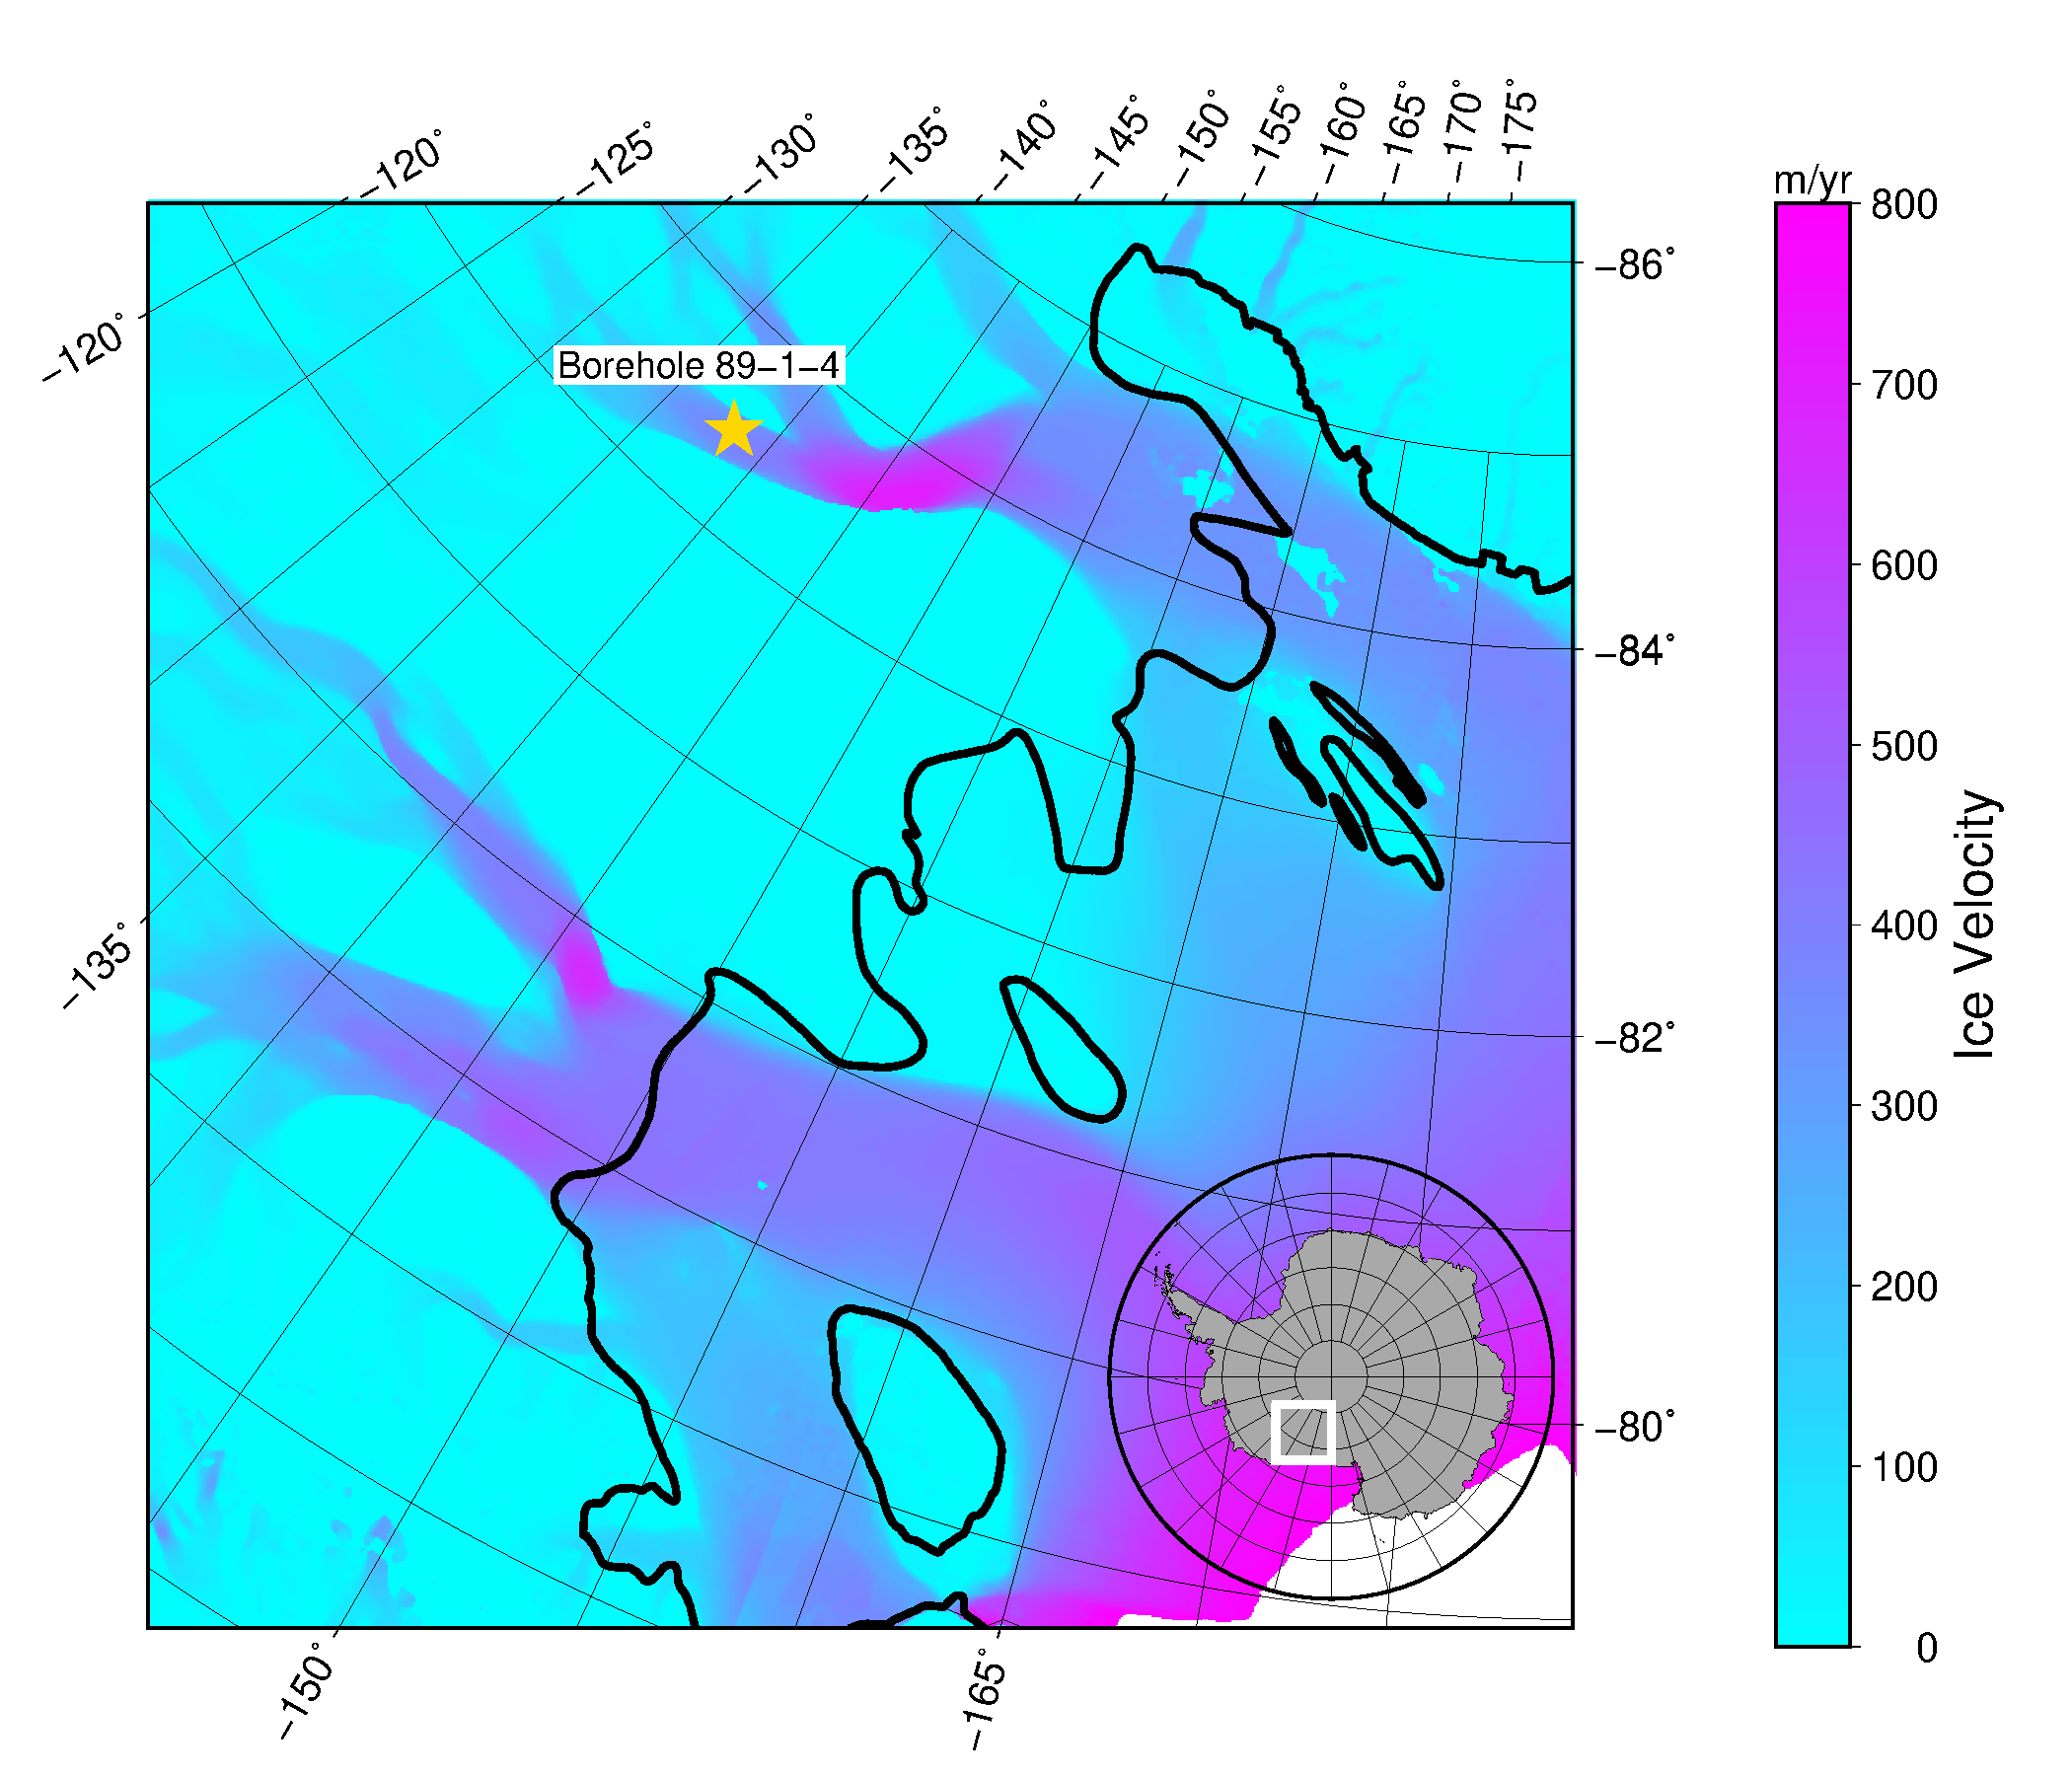
\includegraphics[scale=0.4]{chap_whillans/Figure1.pdf}
   	\caption{Samples for this study were obtained from borehole 89-1-4 near the junction of the B1 and B2 branches of Whillans Ice Stream. Ice velocities of ~600 m/yr are typical in the region [Rignot et al., 2011; Mouginot et al., 2014]. The grounding line is marked in solid black.}
  	\label{}
\end{figure}
% End Figure %

% Figure %
\begin{figure}
	\centering
		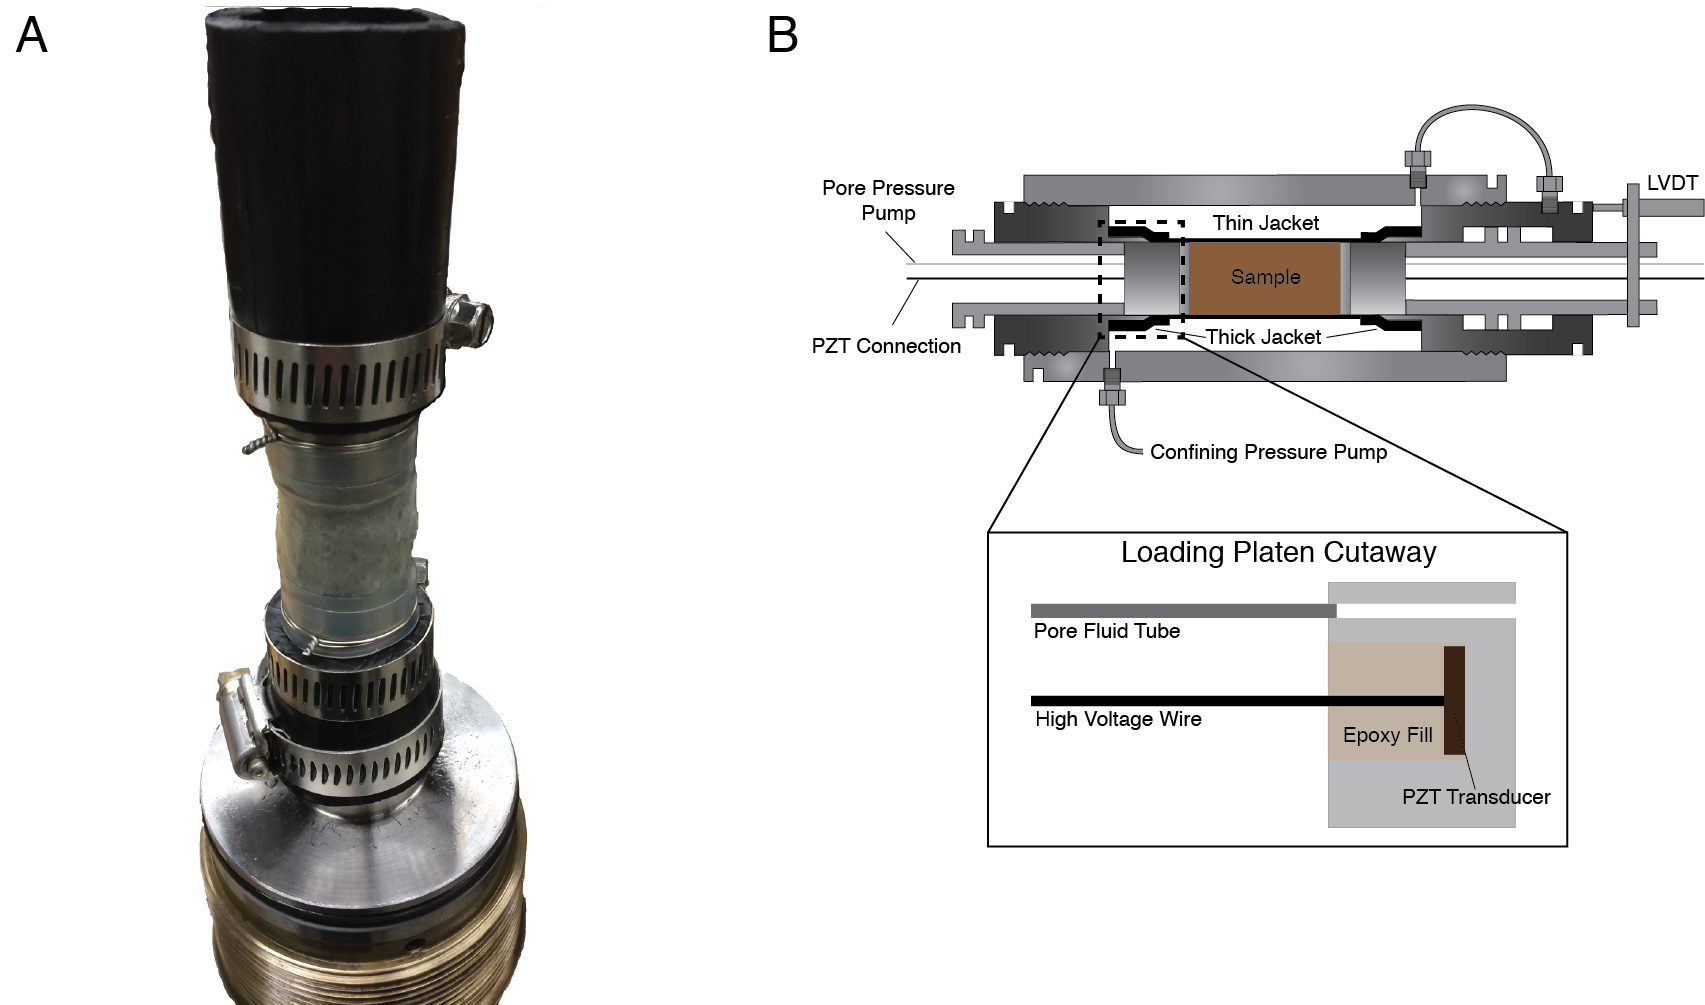
\includegraphics[scale=0.5]{chap_whillans/Figure2.png}
   	\caption{A) The completed sample assembly ready to be loaded into the pressure vessel. B) Schematic diagram of the tri-axial loading cell. Heat shrink tubing was used as a thin, low-strength jacketing material. A hydraulic syringe pump provided isotropic confining and axial loading stresses. A linearly variable displacement transformer (LVDT) measured sample stain. Two high-precision water syringe pumps imposed a hydraulic head to determine sample permeability. Piezoelectric transducers in the loading platens measured the elastic wave travel time through the core (inset). }
  	\label{}
\end{figure}
% End Figure %

% Figure %
\begin{figure}
	\centering
		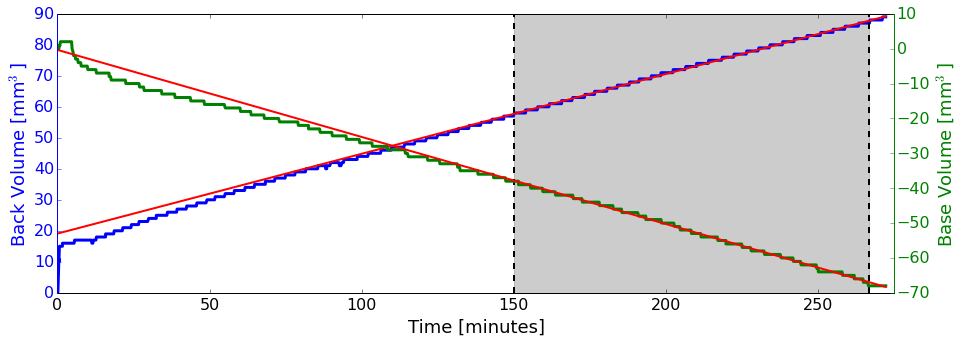
\includegraphics[scale=0.45]{chap_whillans/Figure3.png}
   	\caption{To determine permeability, flow rates from the upstream (blue) and downstream (green) pumps are fit with a least squares fit (red) when the steady-state flow condition is achieved (shaded area). The procedure is repeated at multiple hydraulic heads for repeated permeability measurement.}
  	\label{}
\end{figure}
% End Figure %

\clearpage

% Figure %
\begin{figure}
	\centering
		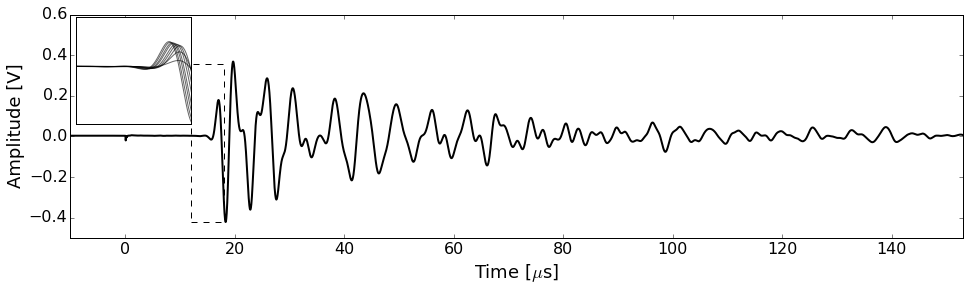
\includegraphics[scale=0.45]{chap_whillans/Figure4.png}
   	\caption{An example acoustic waveform collected during the step-loading test. Inset shows changes in travel time with step loading to 1 MPa effective stress. First arrivals are picked with a cross-correlation technique for consistency. }
  	\label{}
\end{figure}
% End Figure %

% Figure %
\begin{figure}
	\centering
		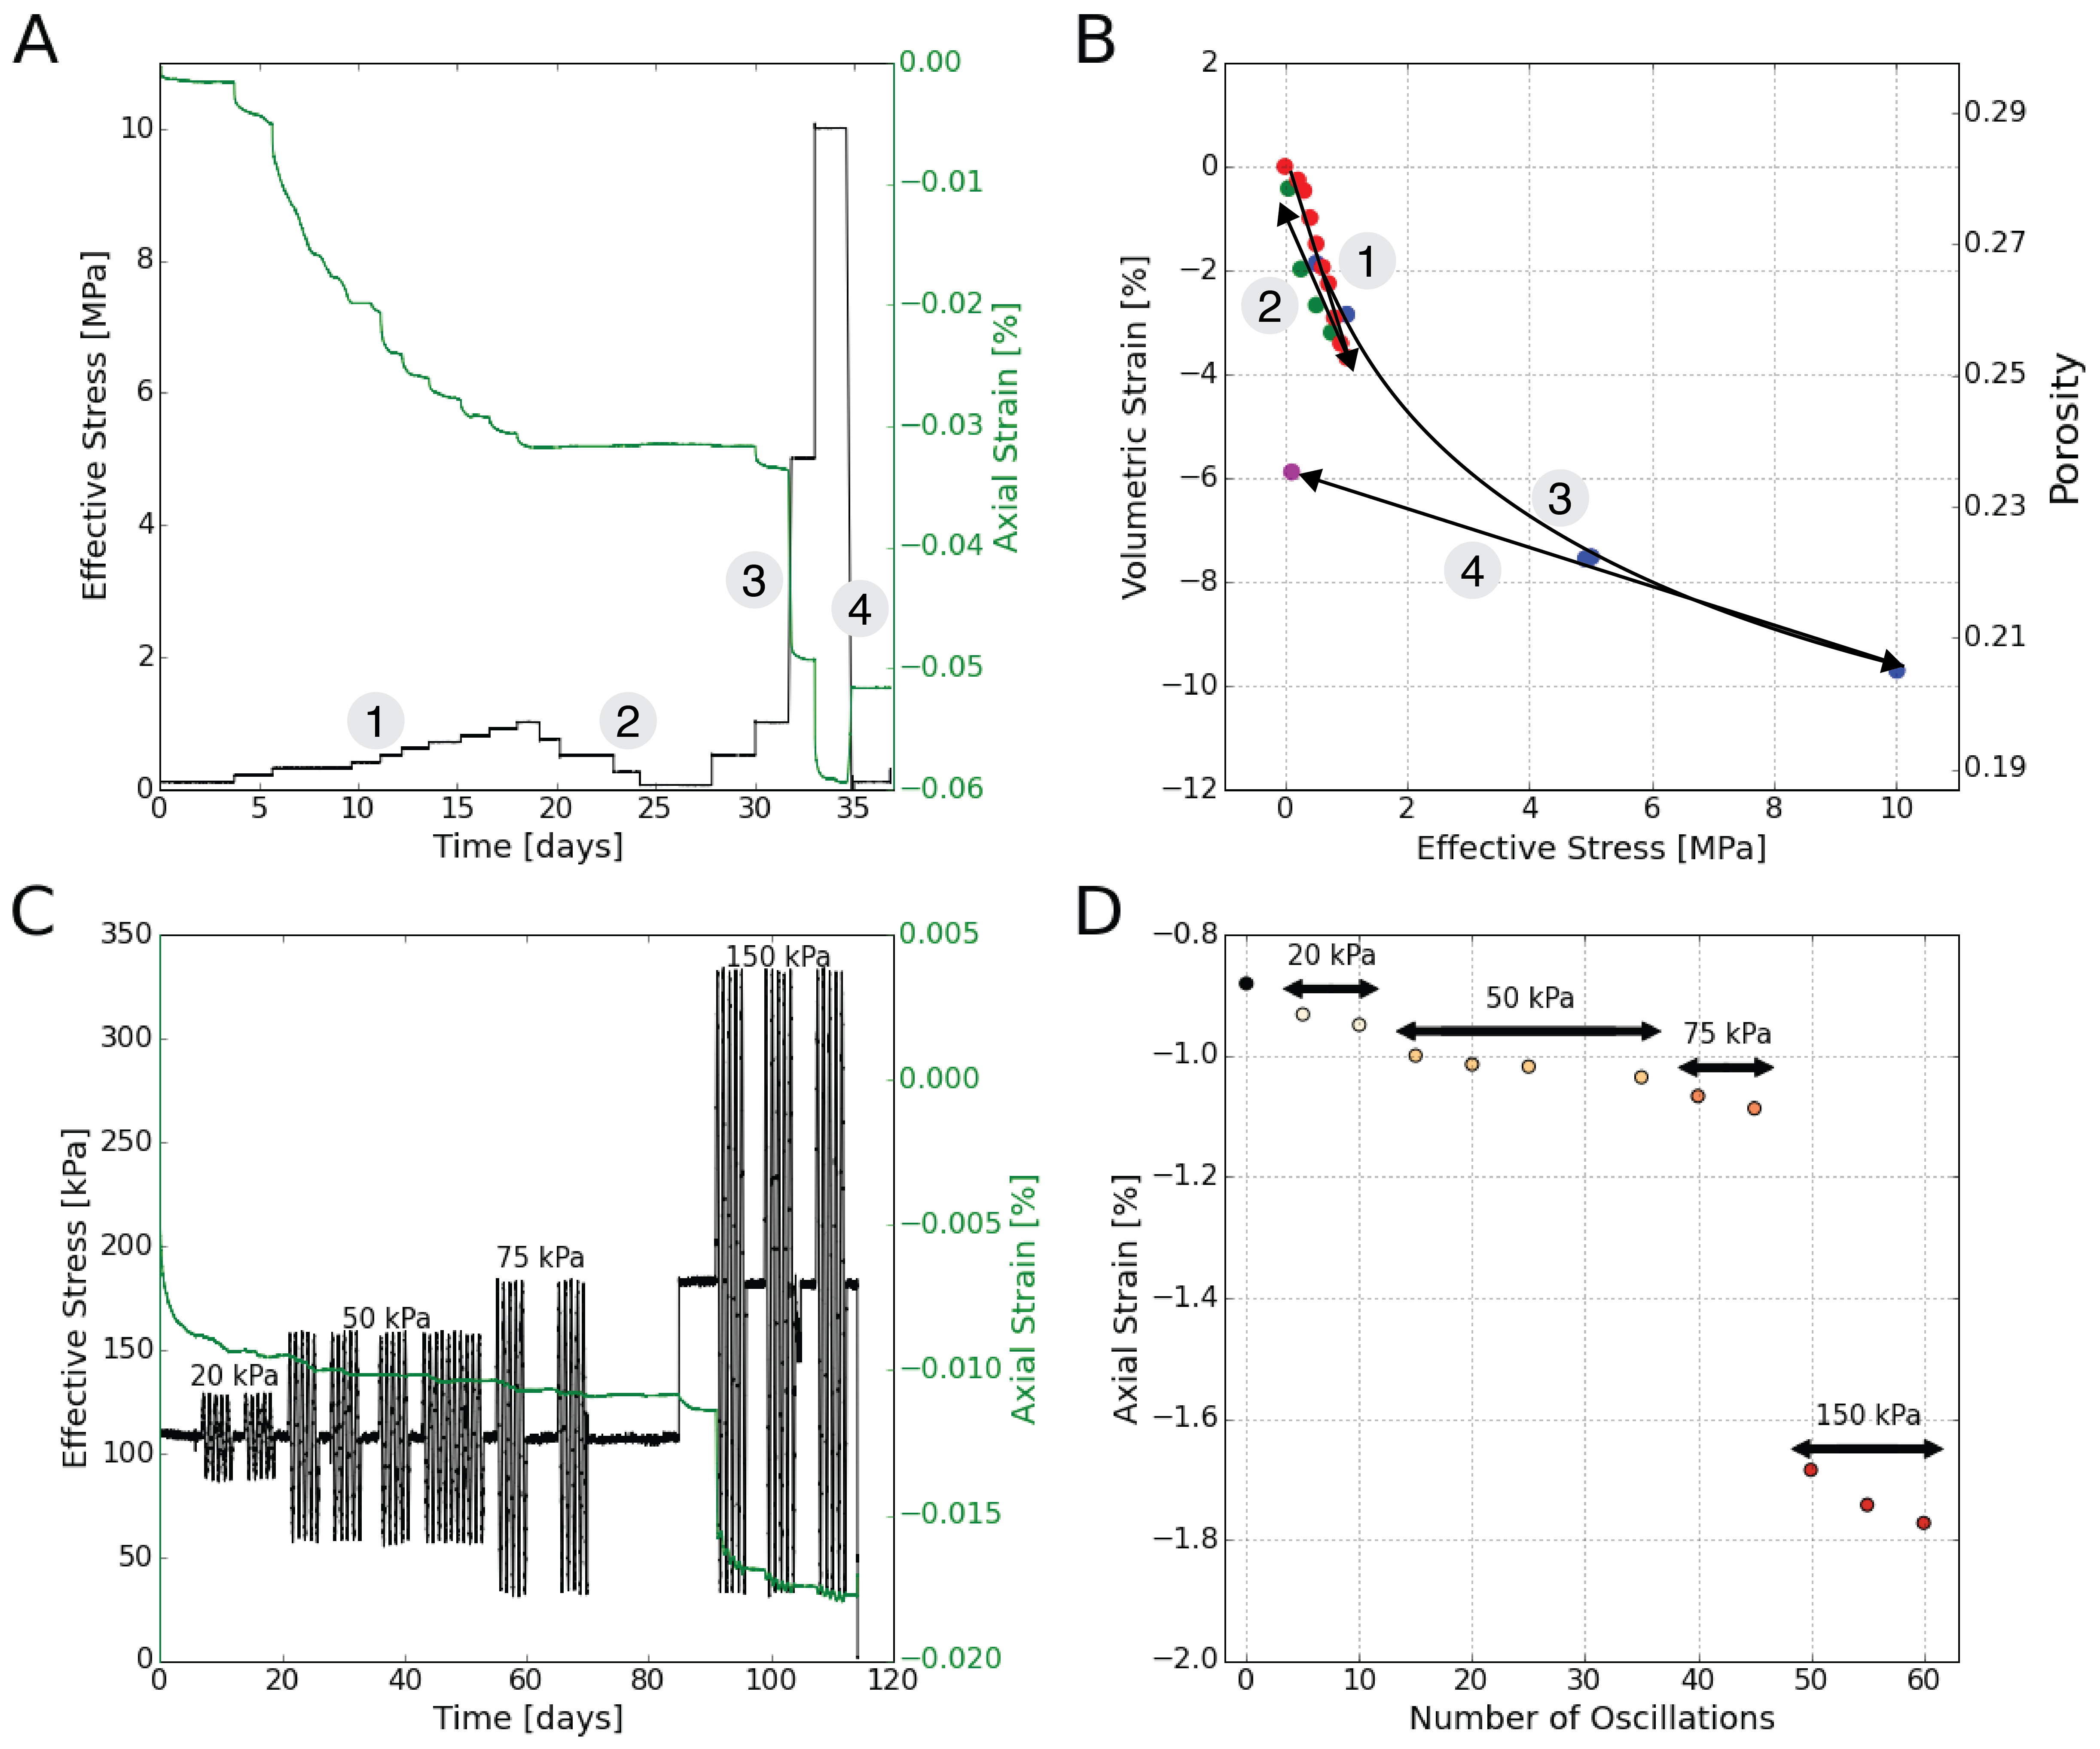
\includegraphics[scale=0.3]{chap_whillans/Figure5.png}
   	\caption{A) Results of the isotropic step loading test show an expected compaction behavior. B) Effective stress and volumetric strain relationship. Initial loading (1) and unloading (2) shows near elastic recovery. Reloading to a 10MPa effective stress (3) created considerable permanent deformation upon the final unloading cycle (4). C) Evolution of axial strain during repeated tidal load cycling. All cycles had a 24-hour period with amplitudes of +/- 25, 50, 75, and 150 kPa. D) Strain was accumulated during all cycle sets, but the additional observed strain decreased with each subsequent set until the amplitude was increased.}
  	\label{}
\end{figure}
% End Figure %

% Figure %
\begin{figure}
	\centering
		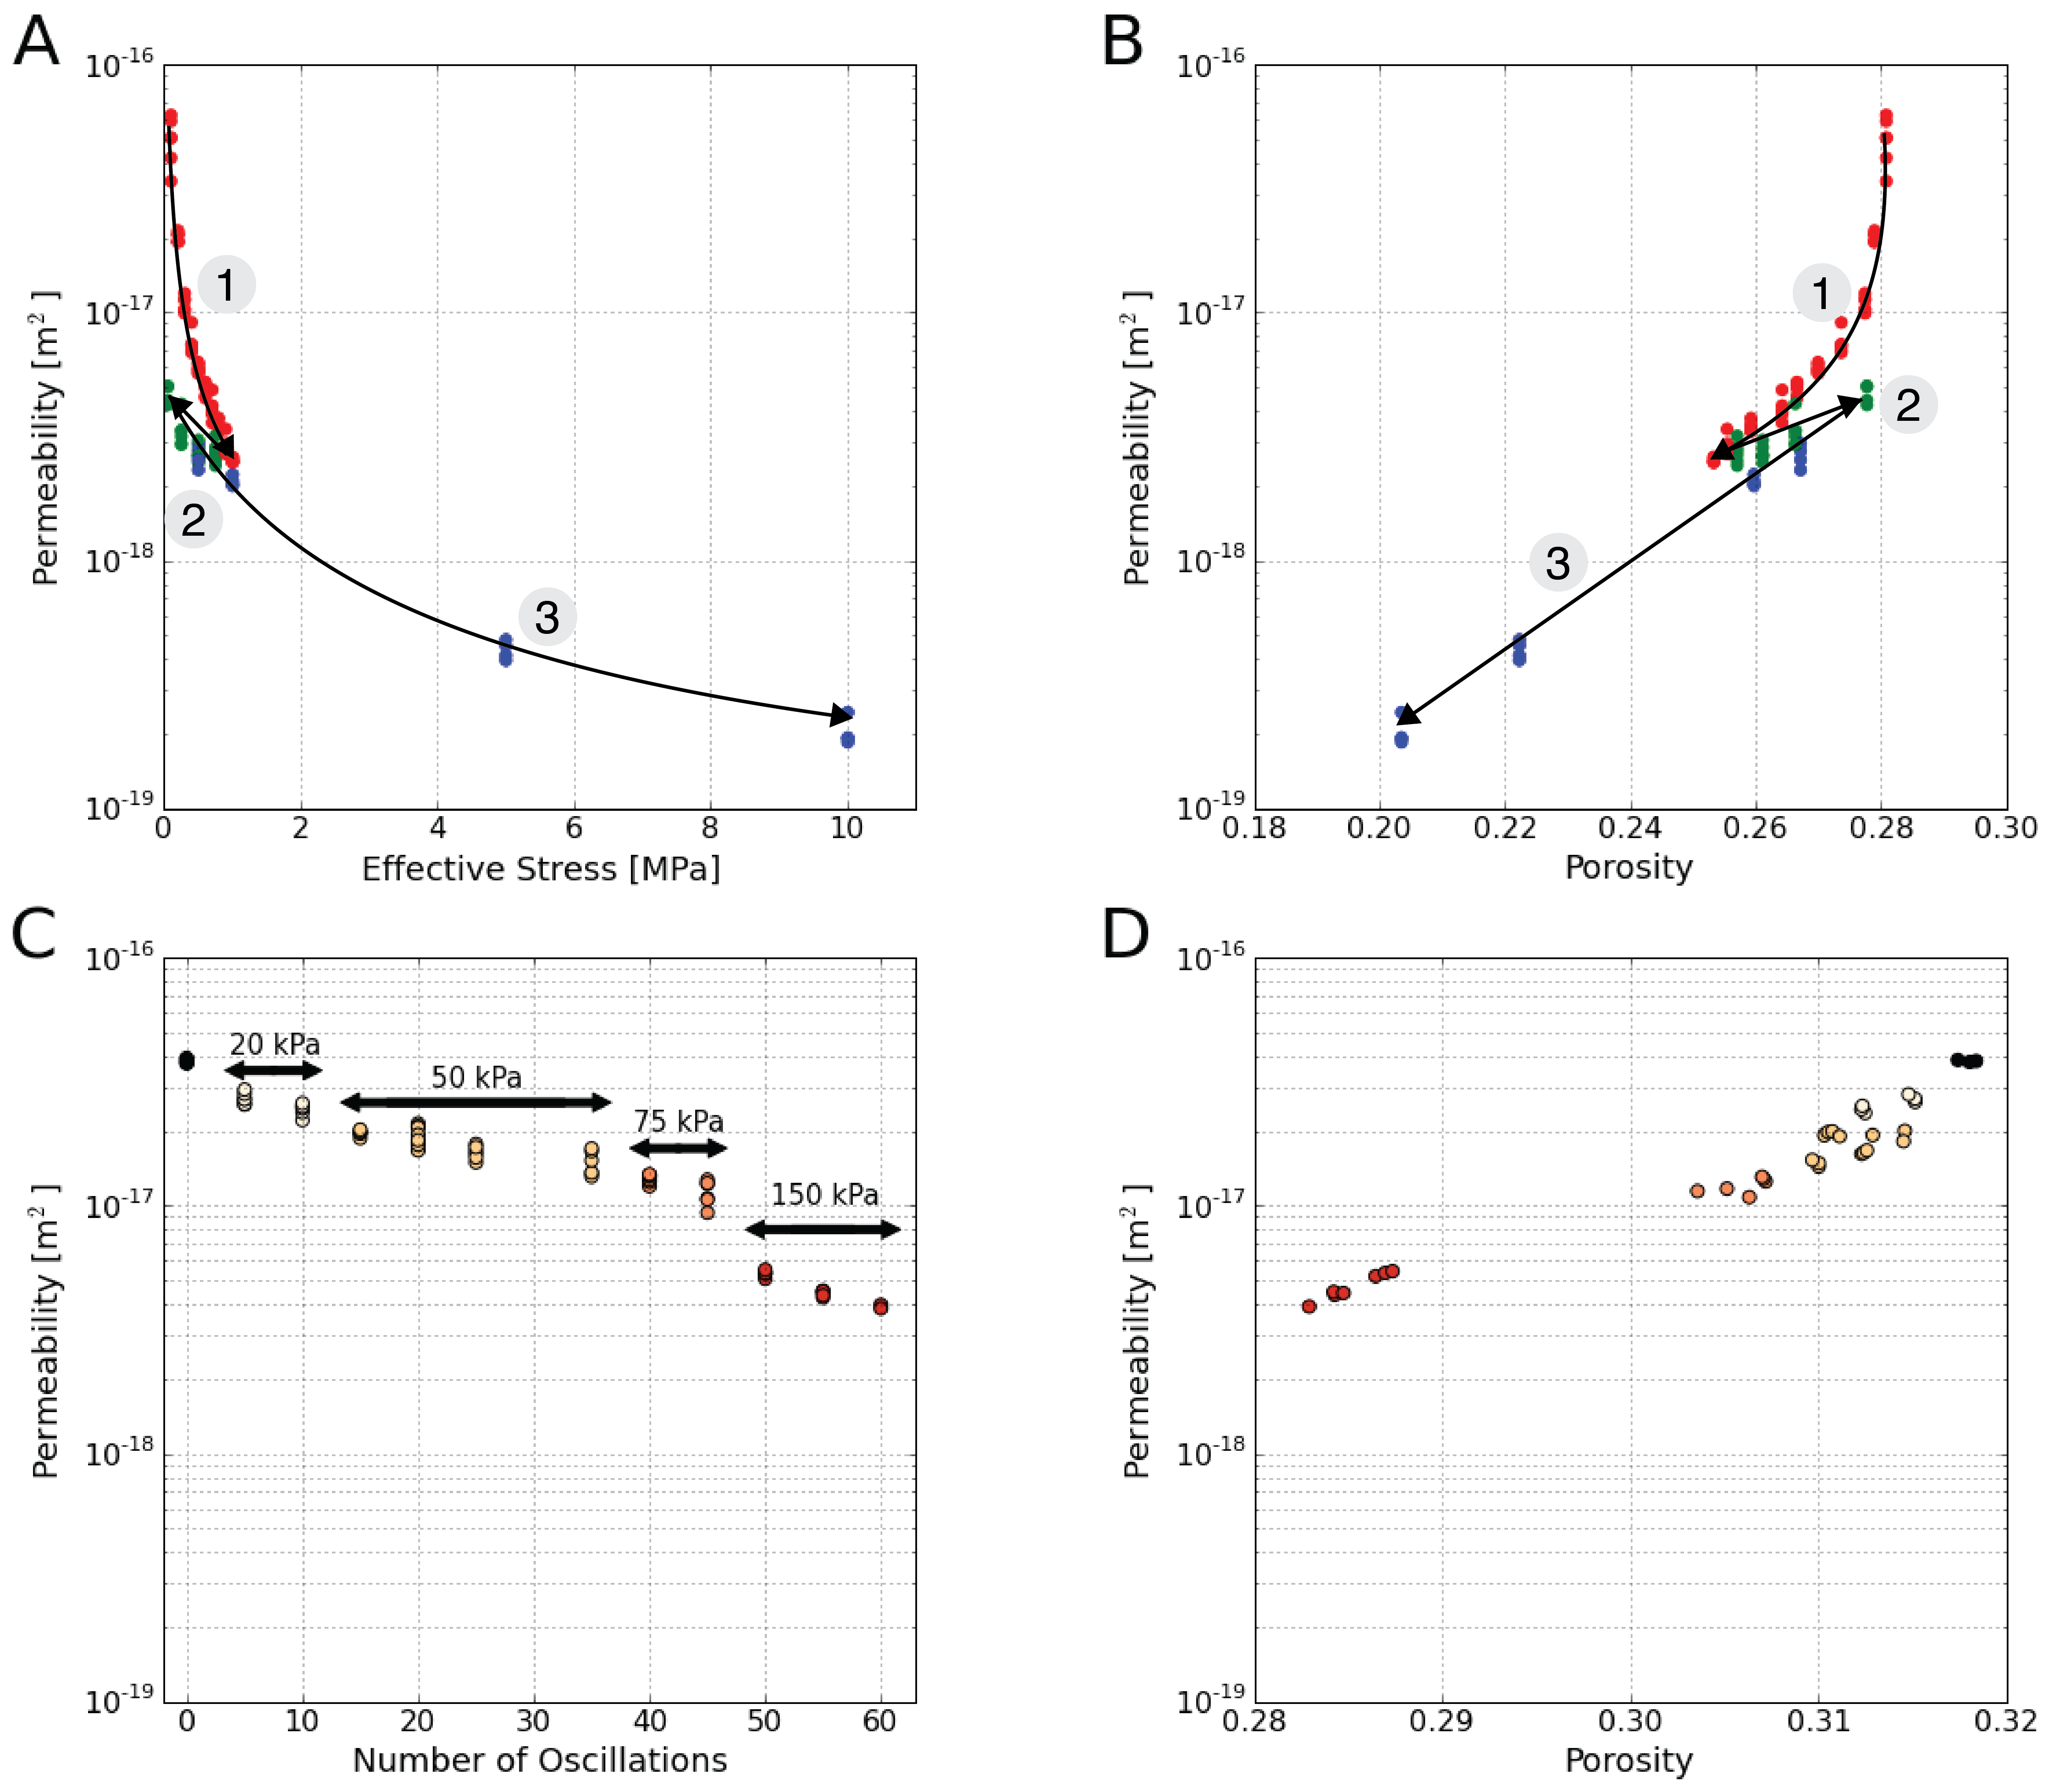
\includegraphics[scale=0.3]{chap_whillans/Figure6.png}
   	\caption{A) Permeability evolution during the step-loading test. Initial permeability values of approximately 3.5�10-17 m2 were reduced by over an order of magnitude during the initial loading (1) with little recovery upon unloading (2). Permeability was reduced by an order of magnitude during reloading (3) to an effective stress of 10 MPa. B) Initial porosity values of 28\% are lower than field estimates. The trend mirrors that of volumetric strain. C) Evolution of permeability and porosity during the tidal loading test indicate that both can be significantly reduced with little additional loading stress, but with load cycling. Initial porosity of 32\% was reduced by several percent over the 60 simulated tidal cycles. D) Permeability was also reduced by an order of magnitude during the cycling. All measurements shown were taken after cycling was complete and the sample had equilibrated.}
  	\label{}
\end{figure}
% End Figure %

% Figure %
\begin{figure}
	\centering
		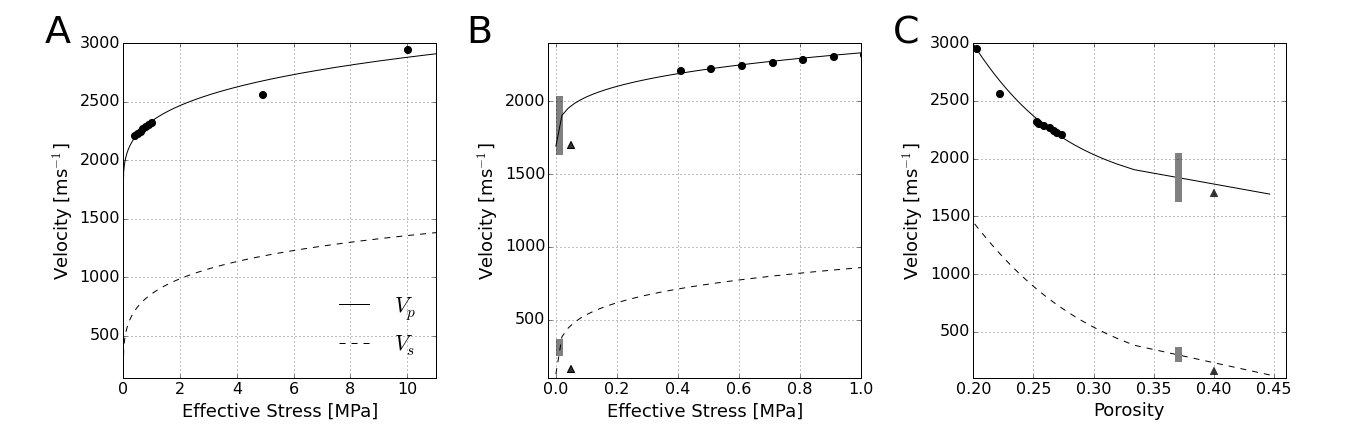
\includegraphics[scale=0.33]{chap_whillans/Figure7.png}
   	\caption{(A) Predicted compressional and shear wave velocities from the effective medium model as a function of effective stress, (B) an expanded view showing field velocity measurements from seismic experiments, and porosity (C). The model is supported by experimental compressional wave velocity measurements, but no shear wave measurements could be obtained in the laboratory due to the very low effective pressures of the experiment. Black circles represent direct measurements from the laboratory, gray bars are velocity estimates by Luthra et al. [2016] and black triangles are estimates by Blankenship et al. [1987].}
  	\label{}
\end{figure}
% End Figure %

\clearpage

% Figure %
\begin{figure}
	\centering
		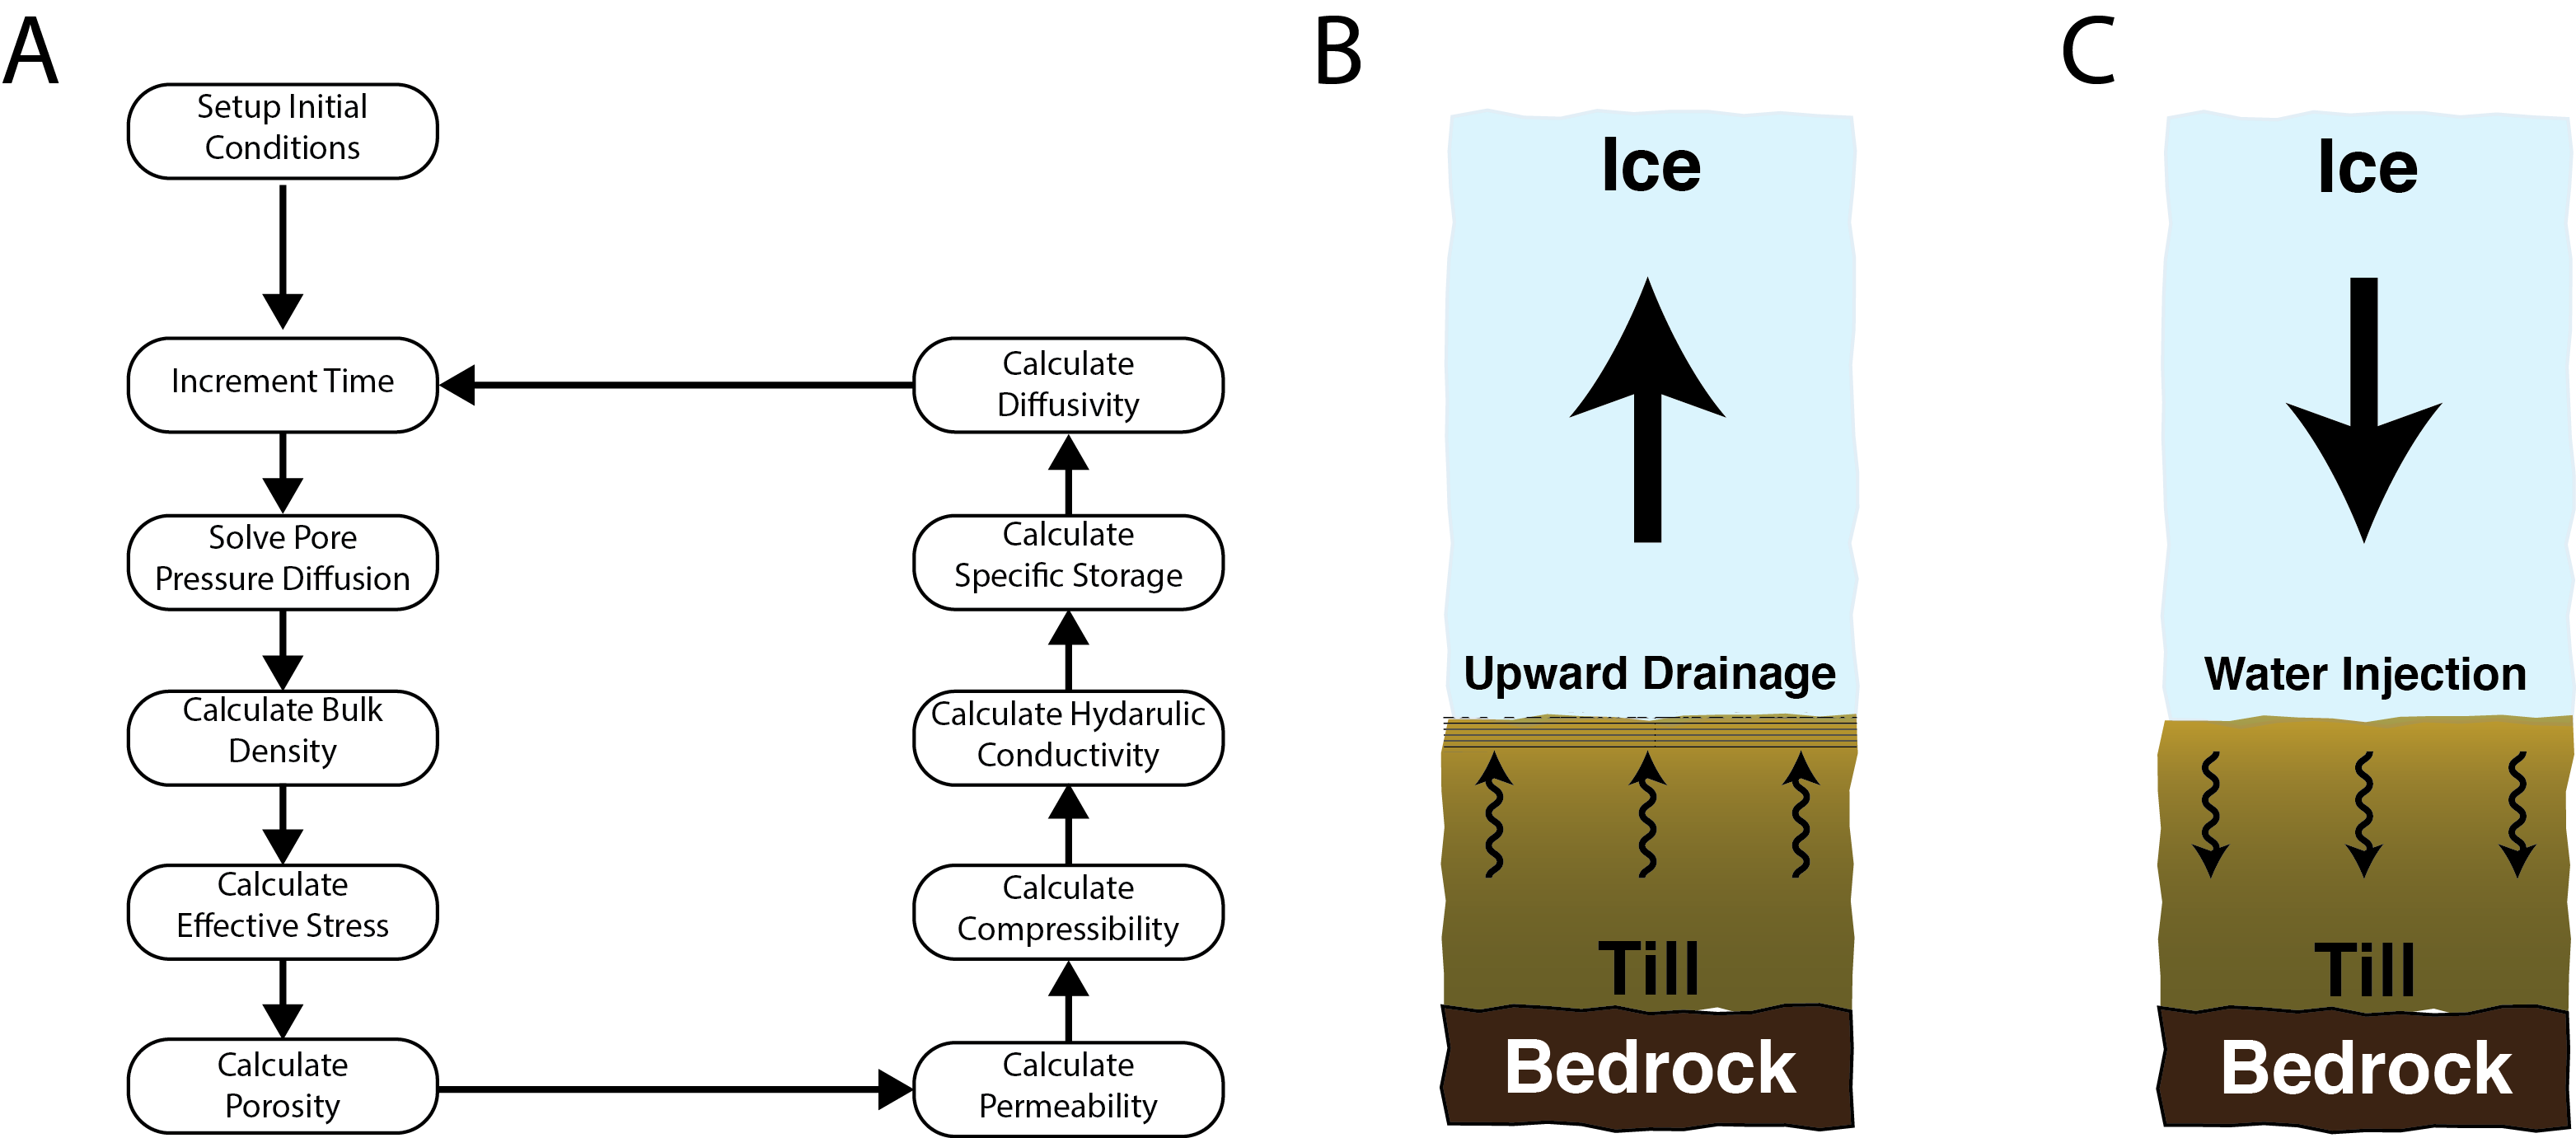
\includegraphics[scale=0.5]{chap_whillans/Figure8.png}
   	\caption{A) Flow chart showing the sequence used when computing the 1-D hydrologic model. B) A cartoon version of the system with ice unloading the till beneath it on a tidal timescale. Upward drainage as a result of lower effective stress at the ice-till interface will quickly result in the formation of a hard layer that slows further drainage and limits the hard layer depth to tens of centimeters. C) Loading from the ice will inject water back into the till as the basal hydraulic pressure is increased.}
  	\label{}
\end{figure}
% End Figure %

\clearpage

% Figure %
\begin{figure}
	\centering
		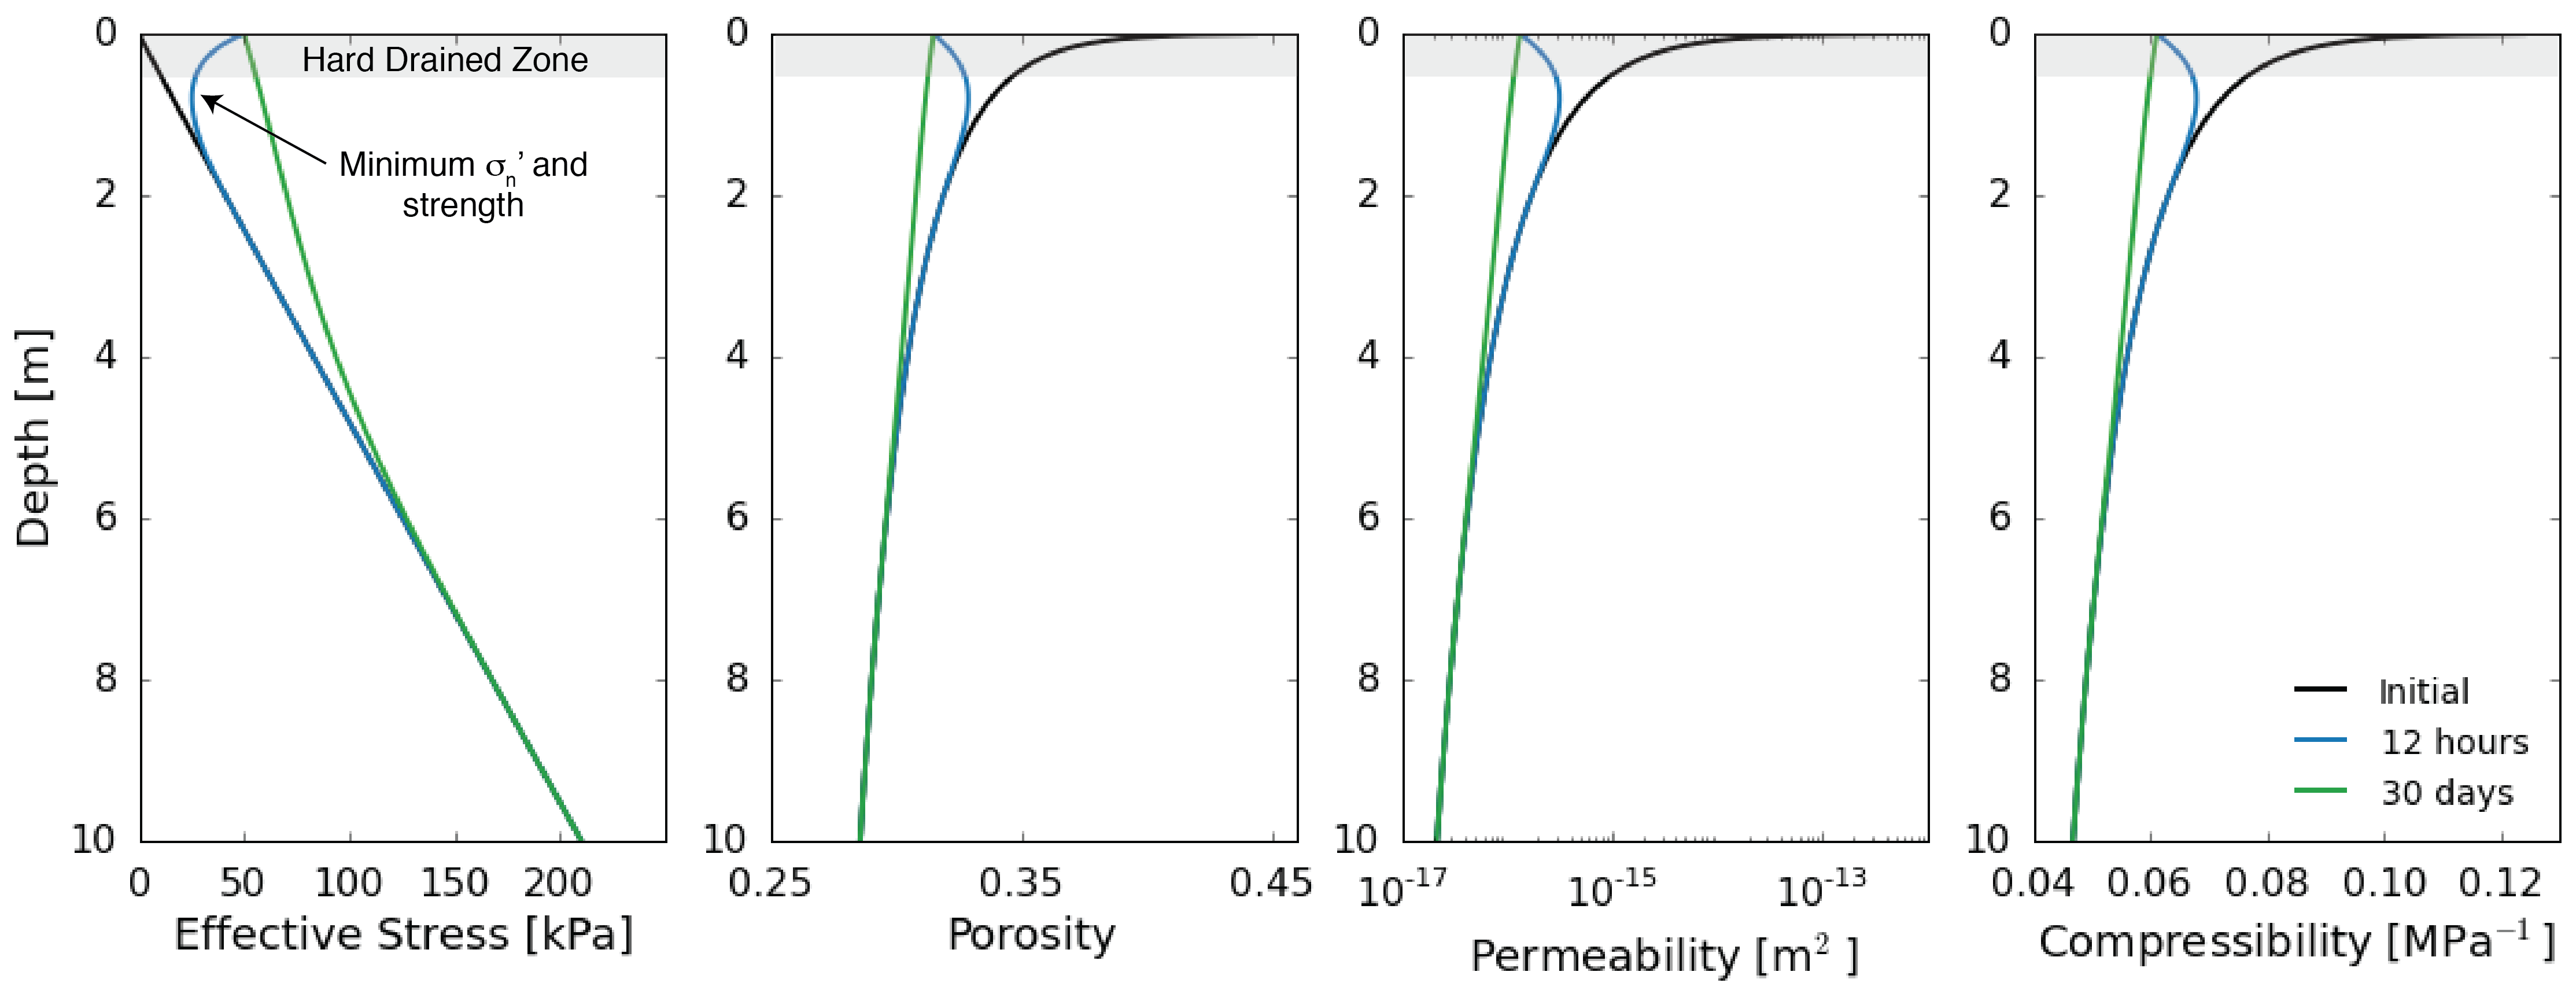
\includegraphics[scale=0.4]{chap_whillans/Figure9.png}
   	\caption{Model results for a coupled diffusion/compaction model of the till layer with an imposed 50 kPa effective stress perturbation at the top boundary.  The perturbation can affect the till over several tens of centimeters in a 12 hour tidal time scale. Over a longer perturbation, such as moving over a rough area on the bed, the till can come close to equilibrium in a month. }
  	\label{}
\end{figure}
% End Figure %

% Figure %
\begin{figure}
	\centering
		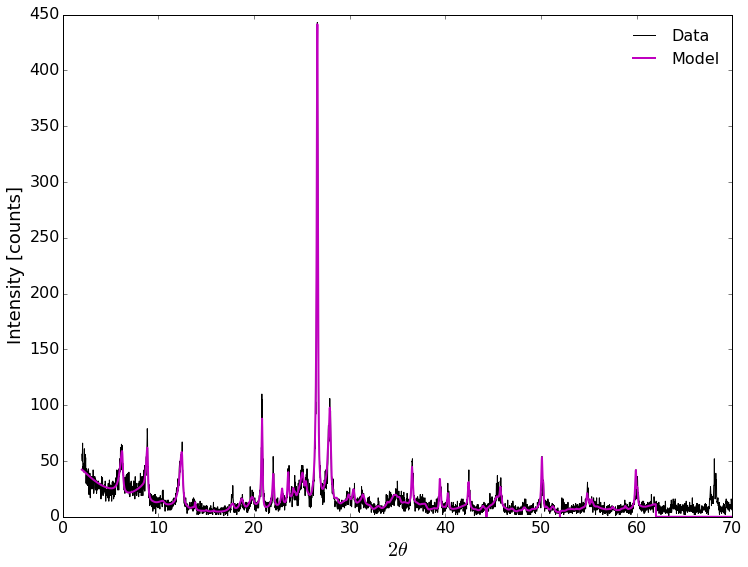
\includegraphics[scale=0.5]{chap_whillans/FigureS1.png}
   	\caption{XRD analysis shows very high clay content in the till samples with significant amounts of quartz as well. Some non-uniqueness exists in the type of clays present, but an effort was made to minimize the misfit with reasonable geological constraints.}
  	\label{}
\end{figure}
% End Figure %

\clearpage

% Figure %
\begin{figure}
	\centering
		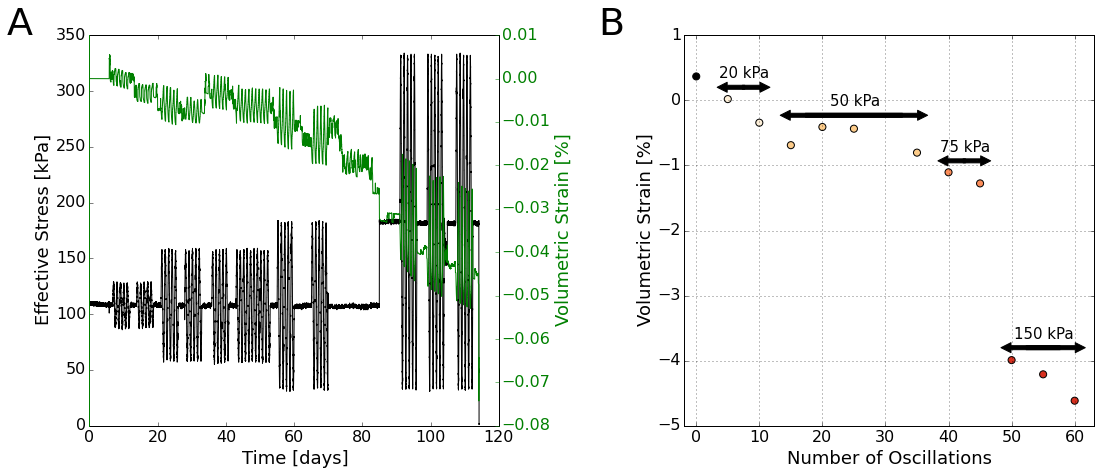
\includegraphics[scale=0.33]{chap_whillans/FigureS2.png}
   	\caption{A) Evolution of volumetric strain during repeated tidal load cycling. B) Strain was accumulated during all cycle sets, similar to the axial strain trends, but with some slight anomalies likely induced by thermal effects on pump volume measurements as volume changes are very small.}
  	\label{}
\end{figure}
% End Figure %

\clearpage

% Figure %
\begin{figure}
	\centering
		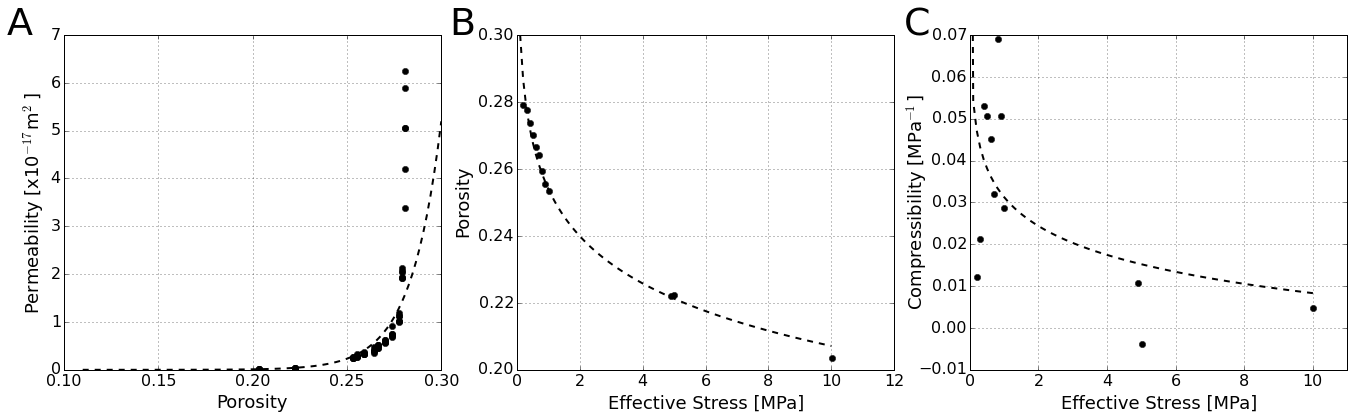
\includegraphics[scale=0.3]{chap_whillans/FigureS3.png}
   	\caption{Experimental data and fits used in loading portions of the simple hydrologic model. Porosity-permeability (A) was fit with an exponential, while effective stress - porosity (B) and effective stress - compressibility (C) were fit with logarithmic relationships.}
  	\label{}
\end{figure}
% End Figure %

\clearpage

\begin{table*}
    \begin{tabular}{|c|c|c|c|c|}
    \hline
    Mineral & Volume Percent & Bulk Modulus [GPa] & Shear Modulus [GPa] & Density [kg/m3]\\
\hline
Quartz & 23.73 & 36.6 & 45 & 2650\\
\hline
Clay & 50.49 & 48 & 20 & 2626\\
\hline
Feldspar & 25.78 & 76 & 26 & 2560\\
    \hline
    \end{tabular}
    \caption{Physical parameters used to construct the effective medium model of compressional and shear wave velocities. Values are based on Dvorkin [1999] and Wang [2001].
}
\end{table*}












\chapter{On the origin and evolution of electrical signals\\ during frictional stick slip in sheared granular material}

\section{Abstract}
Electromagnetic signals have been reported in association with geophysical phenomena including earthquakes, landslides, and volcanic events. Mechanisms that suggested to explain seismoelectrical signals include triboelectricity, piezoelectricity, streaming potentials, and the migration
of electron holes, yet the origin of such phenomena remains poorly understood. We present results from laboratory experiments regarding the relationship between electrical and mechanical signals for frictional stick-slip events in sheared soda-lime glass bead layers. The results are interpreted in the context of lattice defect migration and granular force chain mechanics. During stick-slip events, we observe two distinct behaviors delineated by the attainment of a frictional stick-slip steady state. During initial shear loading, layers charge during stick-slip events and the potential of the system rises. After steady state stick-slip behavior is attained, the system begins to discharge. Coseismic signals are characterized by potential drops superimposed on a longer-term trend. We suggest that the observed signal is a convolution of two effects: charging of the forcing blocks and signals associated with the stress state of the material. The long-term charging of the blocks is accomplished by grain boundary movement during the initial establishment of force chain networks. Short-term signals associated with stick-slip events may originate from produced electron holes. Applied to tectonic faults, our results suggest that electrical signals generated during frictional failure may provide a way to monitor stress and the onset of earthquake rupture. Potential changes could produce detectable signals that may forecast the early stages of failure, providing a modest warning of the event.

%% ---------------------------------- %%
%
%  Introduction
%
%% ---------------------------------- %%

\section{Introduction}

A number of electromagnetic signals have been observed during tectonic faulting and mechanical failure of rocks, but the mechanisms underlying these phenomena are still unclear.  Recently, efforts to couple observations by the physics and materials science communities with observations of natural phenomena in the geoscience community have begun to show promise \citep{YujiEnomoto:2007tq,Balk:2009hu,Takeuchi:2010kc,Freund:2010bl,Onuma:2011ii,Shinbrot:2012jd}.  Existing studies indicate that large earthquakes are, in some cases, preceded or accompanied by ultra low frequency electromagnetic emissions, residual magnetic anomalies, and even visible electrical atmospheric discharges known as `earthquake lights' \citep{Derr:1973tq, Park:1993vi, Uyeda:2009du}.  Understanding these phenomena may improve our ability to provide early warning of seismic events or other hazardous material failures, and will provide insight into fault zone physical processes and stress conditions during the seismic cycle.  

Several mechanisms have been proposed to explain the generation of electrical potentials in Earth, including: piezoelectric effects, streaming potential, contact/tribo electrification, fracto-emission, plasma excitation, and semiconductor-like effects \citep{Finkelstein:1973vz,Dickinson:1982hx,Dickinson:1982uy,Dickinson:1984ft,Freund:2000vf, Frid:2000vn, Jouniaux:2013da,Takeuchi:2013cu}.  Even with an assumed mechanism of charging, there are still many mysterious aspects of the phenomenon, including conduction of the charge to the surface, charge residence time, and Earth/atmosphere interaction. Here, we examine electrical potentials observed for sheared granular layers that exhibit regular frictional stick-slip instabilities in the laboratory.  We interpret the results of experiments on this fault gouge analog in the context of modern theories of charge separation in geologic materials. 

%% ---------------------------------- %%
%
%  Previous Work
%
%% ---------------------------------- %%

\section{Previous Work}

\subsection{Natural Occurrences}
Light emissions have been reported in association with rock failure during both seismic rupture at Earth's surface (so-called Earthquake lights) and during rock bursts in mines.  Earthquake lights have been reported during various stages of the seismic cycle, in addition to other electromagnetic phenomena.  Related electrical phenomena believed to be connected with rock failure include ultra low frequency electromagnetic emissions, resistivity variations \citep{Park:1993vi}, and anomalous animal behavior \citep{Kirschvink:2000wu}.  A summary of these phenomena by\citet{Uyeda:2009du} and the references therein illustrate the breadth of observations.

The first photographically well-documented sequence of earthquake lights (EQL) occurred during the 1965-1967 Matsushiro earthquake swarm \citep{Derr:1973tq}.  Earthquake lights were also observed in the M7.2 November 29, 1975 Kalapana earthquake.  The M7.2 1995 Kobe earthquake was reported to have EQL as well as observations of burned plant roots at the rupture site, and natural remanent magnetization (NRM) anomalies \citep{YujiEnomoto:2007tq}.  Anomalous NRM have been measured in pseudotachylyte, suggesting that high remanent magnetizations were acquired in a co-seismic electrical process and locked into thin, rapidly cooling layers of melt \citep{Ferre:2005ci}.  Visual electromagnetic phenomena were reported before the M6.3 April 6, 2009 L' Aquila earthquake \citep{Fidani:2010ie}. Although reports were confused by astronomical/meteorological events and coseismic power line flashes, a number of unexplained observations remain.

Most reported EQL have been generated on intraplate faults with relatively shallow sources, for magnitude 7 and greater events, and commonly for earthquakes with demonstrated surface rupture.  \citet{Lockner:1983ux} suggest that vaporization of water produces a charge separation that is then moved to the surface by a central fluid conductor.  Reports of EQL phenomena often include descriptions of the anomalies being most intense at topographic highs, suggesting that surface charge on the ground was concentrated by the topography. EQL may be more common in high stress drop events and/or in association with branching and geometrically complex events \citep{scholz2002mechanics}.

\subsection{Previous Experimental Work}

Much experimental work has been done to test physical mechanisms that could cause electrical anomalies during seismic activity and rock failure.  The most relevant explanations are briefly discussed here, but more in depth discussion may be found in \citet{Uyeda:2009du}, \cite{Freund:2000vf}, and references therein.

Early work by \citet{Nitsan:1977te} investigating piezoelectric effects showed electromagnetic radiation in the 1-10 MHz range during the fracturing of quartz bearing rocks under uniaxial compression.  The idea of the piezoelectric effect causing changes in the electrical field during failure suggested that frequency content of the signal would be related to the rate of stress release.  This relationship is supported by a spectral shift to higher frequencies with smaller particles \citep{Nitsan:1977te}.  Uniaxial compression studies using cores of Red Texas Granite, Barre Granite, Dakota Sandstone, Carthage Marble, and quartzite exhibited electromagnetic signals peaking below 40 kHz in association with failure. Observed signals also exhibited some degree of directionality \citep{Rowell:1981tp,Hanson:1982vu}.  Signals peaking at 100 kHz were observed during impact and cratering tests by \citet{Bianchi:1984vf} both in vacuum and at atmospheric pressure.

Mechanisms involving the formation of cold plasmas during fracture and impact have also been proposed to explain charge generation \citep{Martelli:1985wv}, but have not been investigated thoroughly.  Calculations considering a beam-plasma interaction producing an ion-acoustic instability suggest that the expected radiation frequencies are at $\sim$50 kHz.  

A recent study by \citet{Onuma:2011ii} examined gabbro and quartz powders, used as simulated fault gouge and sheared between gabbro forcing blocks in a saw-cut geometry.  Electrical signals in the co-seismic period were detected by direct contact electrodes as well as toroidal induction coils surrounding the sample.  In 25\% of their experiments, a possible pre-cursory signal was detected, but not consistently on all instruments.  Piezoelectricity was ruled out as a dominant mechanism, because signals were observed in piezoelectric and non-piezoelectric gouges and there was no preferred c-axis orientation in the quartz powder.  Signals were observed from piezoelectric and non-piezoelectric materials by \citet{Cress:1987wy} as well, but in their experiments on quartz produced larger signals than other materials.  \citet{Onuma:2011ii} did not observe signals during initial loading; however, such signals have been observed by other workers in natural and experimental cases \citep{Takeuchi:2010kc} who attributed them to frictional electrification because they scaled roughly linearly with slip.

The presence of moving dislocations with respect to propagation of microcracks producing a `pressure stimulated current'  in marble samples has been examined \citep{Triantis:2008uo}.  These currents are a result of charge separation during the beginning stages of failure, not during the initial loading stages.  

Piezoelectric effects are well-documented in materials such as quartz, but geologic materials are not expected to have the required mineralogy or grain alignment to make this a viable mechanism in nature.  Randomly oriented grains would produce a series of randomly oriented dipoles that would cancel to produce a net-neutral field.  Streaming potentials and electrokinetic effects \citep{Mizutani:1976tn} are well-documented, but are generally not of sufficient magnitude to explain the observed phenomena, because large potentials are difficult to maintain with generally conductive fluids present.  Electrification by relative surface movement (tribo-electrification) is also well-documented \citep{Pingali:2009je,Pahtz:2010cq}, but does little to explain electrical signals produced while contacts are stationary to quasi-stationary. 

Evidence for electrical signals during and possibly as precursors to failure in a low stress environment has been collected \citep{Shinbrot:2012jd} in experiments examining slope failure and crack opening or closing in powdered pharmaceutical materials.  An electrostatic voltmeter (ESVM) like that used in this study was used to monitor rotating and tilting drums of powder as well as flexure of powder layers resulting in opening and closing fissures of the material. 

Another model of charge generation during deformation of geomaterials is the `semiconductor' effect.  In geologic materials, oxygen is generally considered to exist in the O$^{-2}$ valence state, but the more oxidized form O$^-$ is also present in a pair of coupled O$^-$ atoms known as a peroxy defect.  The peroxy link can be broken via mechanical strain such as during passage of a mechanical deformation front in the form of a propagating elastic wave or elastodynamic rupture front. In this case, an electron is sourced in an attempt to satisfy the newly formed electrical imbalance at the site of the broken peroxy bond.  This oxidizes the donor, forming a single defect electron (eq.\ref{peroxy}). \citep{Freund:2000vf, Freund:2006kb,Freund:2010bl}
  
\begin{equation}
O_3 X/^{OO}\backslash YO_3 + [XO_4]^{n-} \leftrightarrow O_3X/^{O} \bullet _O/YO_3+[XO_4]^{(n-1)-}
\label{peroxy}
\end{equation}

Electrons are not free as charge carriers, but holes remain mobile \citep{Freund:2000vf,Freund:2006kb,Freund:2010bl,Balk:2009hu}. The semi-conductor effect has been explored in solids \citep{Takeuchi:2013cu,StLaurent:2006fq}, but few studies have been conducted on granular materials, which are likely to be important in the behavior of tectonic fault zones.

%% ---------------------------------- %%
%
%  Methods
%
%% ---------------------------------- %%
\section{Methods}

We conducted experiments on granular layers used to simulate fault gouge under controlled boundary conditions, with concurrent measurement of electrical potential, stresses, and strains of the layer to explore the relationship between stress state and the evolution of electrical signals.  We used glass beads to represent granular fault gouge because they exhibit repeated frictional stick-slip behavior and share key friction constitutive properties with rock. The main advantage of this choice lies in the reproducibility of stick-slip behavior, allowing investigation and isolation of the processes that cause electrical signals relevant to natural faults containing granular gouge by using a simple, well-characterized system. We note that glass should contain fewer starting defects than silicate minerals found in natural fault gouges, such that any effects observed in our glass bead experiments would likely be amplified in natural materials.

\subsection{Apparatus}

All experiments were conducted on a biaxial deformation machine with a servo-hydraulic control system \citep{Karner:2000tj,Frye:2002jj}.  Hydraulic servo valves are operated in either displacement or force feedback modes through a series of analog amplifiers and comparators.  Control displacement signals are generated by a 16-bit digital to analog converter capable of $\pm 5$V range.  The apparatus (Figure \ref{biax_setup}A) is capable of 1 MN of force on the horizontal ram and 1.5 MN on the vertical ram.  Ram velocity can be controlled to ~0.1 $\mu m/s$ in displacement mode, or to about 10N in load mode \citep{Hong:2005gd,Rathbun:2008ks}.

We used forcing blocks of cast acrylic with a dielectric strength of 15-17 V/$\mu m$ and a tensile strength of 55-77 MPa.  Forcing blocks were cut to size and machined with grooves 1 mm deep and 2 mm wide perpendicular to the shearing direction to ensure that shear occurred within the layer and not at the layer boundary \citep{Anthony:2005jo,Knuth:2007ci}.  Acrylic side shields were also made to confine the sample material. The nominal frictional contact area was 10 cm x 10 cm.

Force was measured using Beryllium-Copper strain gauge load cells built in-house and placed in series with the loading ram and sample. The load cells and the wheatstone bridge electronics are calibrated regularly with a proving ring traceable to the National Bureau of Standards.  Displacement is measured with direct current displacement transducers (DCDTs) affixed to the ram nose and referenced to the end platens of the hydraulic rams.  Positions of both classes of instrumentation are noted in Figure \ref{biax_setup}A. 

We recorded data using a 24-bit, 16-channel simultaneous, delta-sigma style analog to digital system.  Samples are collected at 10 kHz and averaged to the desired rate from 1 Hz to 10 kHz as necessary to maintain the appropriate signal-to-noise ratio.  Recording rates may be changed during the experiment, and our tests show minimal cross-talk or dwell errors in this system.

\subsection{Sample Material \& Preparation}
Samples were built in the double direct shear configuration (Figure \ref{biax_setup}B) using soda-lime glass beads \citep{Anthony:2005jo}.  Two layers of beads were confined in a three forcing block assembly with a rubber membrane at the bottom and side-shields on the boundaries to avoid lateral extrusion of the material.  The top of the sample was unconfined. 

Layers were built by placing the side forcing blocks on a leveling jig and applying cellophane tape around the perimeter.  The tape was then trimmed to the desired height to produce uniform, reproducible layers. We used 5 mm thick layers for all experiments in this study (Table 1).  Sample material was poured into the form, lightly compacted, and leveled.  The center forcing block was affixed to one side block (and the sample) with additional cellophane tape, securing the blocks and gouge layer and providing enough strength to allow transport of the sample from the bench to the deformation apparatus. The process is repeated for the second layer.

We constructed layers using Class IV soda lime glass spheres (product GL0191B4/106-150) from Mo-Sci Specialty Products in Rolla, Missouri (composition shown in Table \ref{bead_composition}).  Two mono-disperse size distributions were tested: 100-150 $\mu m$ and 420-500 $\mu m$. Scanning electron microscopy (SEM) analysis of the beads shows that they are homogeneous, with few exceptions, and smooth (Figure \ref{starting_SEM}). Past work has shown that bead comminution is minimal until $\sigma_n>10$ MPa \citep{Mair:2002hu,Mair:2011fd}.  

\subsection{Potential Measurement}
Electrical potential on the layers was measured by a model 344 electrostatic non-contact volt meter (ESVM) manufactured by Trek Inc.  This instrument reported the potential with respect to system ground sensed in its field of view. An analog output of the measured voltage was divided by 100 to provide a sensing range of $\pm 2$ kV with a $\pm 20$ VDC output signal recorded.  A `response' setting on the instrument controlled internal damping constants.

The sensor head contains two electromechanically oscillated plates.  Plates are fixed parallel to each other with the surface normal facing the surface under test.  The front plate is affixed to the instrument body and has a small aperture in the center. The rear plate is inside the instrument and is the oscillating plate.  The sensor operates by varying the voltage across the plates and sensing the alternating current (AC) signal resulting from the movement of the plates with respect to one another.  When the AC component of the signal is nulled, the voltage across the plates exactly matches the voltage on the surface under test.  This sensor configuration has several advantages: 1) no contact is required with the surface under test, which is excellent for systems where coupling is a challenge, 2) there is no arcing risk since the instrument and surface under test are at the same potential, and 3) the sensor is easily portable, allowing tests with different viewing positions.

Two different sensor geometries were used: side view and top view (Figure \ref{biax_setup}C).  In the top view, all tape between the sensor and the sample was removed.  In the side view, a notch was cut in the side shield, leaving only a thin layer of tape (necessary to prevent extrusion) for the sensor to observe through.  In our calibrations, we found that the sensor operates normally when viewing signals through thin obstacles.  

\subsection{Experimental Procedure}
Samples were placed into the testing machine and normal load of 4 MPa was applied and maintained to compact the layers.  The shear load was then applied by driving the vertical ram at a constant displacement rate (1, 30, or 100 $\mu m/s$).  Electrical potential was recorded by placing the sensor in either the top or side view geometry with a distance of $\sim$1 cm between the front of the sensor and the gouge layer.  The response setting was set to the maximum value of 9.  
	 
We conducted experiments at room (ambient) humidity, at 100\% relative humidity (RH), and under submerged conditions using de-aired water.  100\% RH was achieved by placing the sample assembly in a plastic membrane with a beaker of anhydrous sodium carbonate solution (2:1 ratio with distilled water) within the membrane.  This exothermic reaction produced a 100\% RH environment in the membrane.  For all experiments under controlled humidity, samples were left to equilibrate overnight with a small normal stress applied by a hand-clamp, and then placed in the testing machine. When the experiment began, we refreshed the anhydrous sodium carbonate solution, applied the normal stress and proceeded with our standard loading protocol.  For these experiments, we cut a small window in the humidity-control membrane to provide access for the sensor.  A capacitive sensor hygrometer (Lifft C200 with a maximum error of $\pm3\%$) verified that the relative humidity never fell below 100\%.  Saturated experiments were performed in a similar manner, but the membrane was filled with distilled water and the sample allowed to saturate as load was applied.  The water level just covered the top of the blocks and a top-view ESVM geometry was employed. 

\subsection{Calibration and Control Tests}
We performed tests to ensure calibration of the ESVM, as well as to evaluate the sensitivity of the response control.  The ESVM probe was affixed to an electrically insulating base and placed approximately 1 cm from an aluminum plate.  The plate was charged with a precision DC power supply (HP 6216B) and the true and measured plate voltages recorded. Performance was further evaluated by attaching the surface under test to a function generator.  Square waves were measured on each response setting (1-9) to evaluate ringing of the instrument (Appendix A).

In addition, an experiment identical to those testing electrical potential on the layers was performed with the ESVM pointed away from the load frames into the room and towards a DC charged aluminum plate.  This test was performed to ensure that the signals we observed during shearing were not from electrical interference of the hydraulic control electronics or measurement/recording electronics.  We note that our records include motion of the vertical hydraulic ram when it was not in contact with the sample, and no change in voltage was seen.  This further indicates that no DC offsets or interference were experienced by the ESVM from the testing machine and/or control electronics and transducers.


All calibration and control tests were conducted with identical analog to digital conversion hardware as the experiments.  ESVM calibration tests were also conducted on an independent logger (the LabJack U6) to ensure there was consistent performance and minimal measurement burden from either system.


\subsection{Data Analysis}

Changes in electrical voltage during stick-slip events were picked by hand to evaluate the electrical signal.  ESVM data are more noisy than the mechanical data and electrical anomalies are not found with every stick-slip event, making manual picking the most accurate.  Measured electrical potential and shear stress were plotted on the same x-axis and mouse position clicks were recorded.  Interpretation was aided by superposition of a smoothed potential signal.  The potential was smoothed using a Savitzky Golay filter \citep{SG1964}, as it preserves peaks, but decreases noise.  With the Savitzky Golay filter, a line of specified low-order is fit to a certain data window using a linear least squares technique.  The analysis is then stepped forward and fit signals convolved.

 Data were recorded in a binary form, decoded, converted from bits to engineering units through use of calibrations derived from our transfer standards, and then written out as either a binary or ASCII for analysis. The Python environment was used for processing and analysis.  All stick-slip events were automatically picked by first computing the smoothed derivative of shear stress with respect to time using a running-average slope tool.  Zero-crossings of the derivative indicate a slope change from positive (like that during load up) to negative (like that during failure) or the reverse.  The automatically determined stress drops were checked against a threshold value to ensure that no noise was picked as events.  Automatic picks were visually inspected to ensure algorithm performance.  

\section{Results}

\subsection{Mechanical Data}
The application of shear load resulted in a characteristic linear-elastic stress-displacement record during initial run-in (Figure \ref{ss_humidity}).  Stick-slip behavior began as we reached the failure strength of the material.  As shear load increased during the stick-slip cycle, the material began to creep and deform elasto-plastically, as indicated by deviation of the stress-strain curve from the initial, linear-elastic trend.  When the ultimate strength of the layer was reached, layers failed and a stress drop was observed.  We define the stress drop as the magnitude of shear stress change during stick-slip failure.  In a series of repeating events, we define the recurrence time as the time between peak stresses of two slip events.  For a summary of this terminology see Figure \ref{ss_humidity} inset.  Mechanical steady-state (not to be confused with steady-state frictional sliding) refers to the system state after the initial run-in period, defined as the point at which stress drops in repeated stick-slip events become constant.

All experiments exhibited a maximum coefficient of friction during mechanical steady-state ($\mu \equiv \tau / \sigma_n$) of 0.3-0.4.  For experiments at 100\% humidity or water saturated, we observed an increased stress drop and ultimate strength due to the activation of chemo-mechanical mechanisms such as solution-reprecipitation \citep{Frye:2002jj, Yasuhara:2005ku, Scuderi:2013}.

The recurrence time between events has been shown to vary with load point velocity \citep{Karner:2000tj,Beeler:2001tj}.  We observe a power law relation between load point velocity and recurrence time with a characteristic slope of -1.14 (Figure \ref{ss_props}A).  For faster load point velocities, there is less time for contact healing to occur before the layer fails, resulting in lower maximum stresses and shorter recurrence times.  Shorter healing times also result in smaller stress drops, which produce a correlation between longer recurrence times and larger stress drops (Figure \ref{ss_props}B).  

Experiments performed using the 420-500 $\mu m$ glass beads exhibited repeated stick-slip behavior and a lower coefficient of friction of $\sim 0.2-0.3$.  The occurrence of stick-slip events was less regular than that of the 100-150 $\mu m$ experiments, as there were five times fewer beads spanning the same 5 mm layer thickness.  For the larger beads, we conducted experiments only at 30 $\mu m/s$ and we did not explore the role of loading velocity.  Due to the large stresses applied to the acrylic forcing blocks by the large beads, some chipping of the grooves was observed, so no further experiments were conducted. 

\subsection{Electrical Data}
During shearing we observe two common signals in the electrical potential.  The first is characterized by a long period signal (lasting for the entire experiment) that is a general charging/discharging trend (Figure \ref{electrical_runplot}).  The magnitude of this varies between experiments, but can be as much as 250 V.  The second is characterized by signals that are of smaller magnitude and shorter duration. These are superimposed on the long-term trend, and are synchronous with individual stick-slip events.  The polarity of these events (co-seismic charging or discharging) varies systematically during an individual experiment.  During the initial charging stage of the experiment, prior to reaching mechanical steady-state sliding, the anomalies are generally positive.  During the phase of overall discharging, the electrical anomalies coincident with stick-slip are generally negative.  There are occasional events of unexpected polarity, but there is a strong polarity preference based on the stage of the long-term trend.  We consistently observed that the long-term charging/discharging trends were marked by the attainment of mechanical steady-state (Figure \ref{electrical_runplot}).

After reaching mechanical steady-state, the electrical anomalies associated with each stick-slip event varied systematically with loading velocity (Figure \ref{electrical_zooms}).  For experiments subject to loading at 1 $\mu m/s$, voltage increased by 1-2 V during shear loading between stick-slip events and then dropped rapidly during co-seismic failure.  Similar behavior was observed at 30 $\mu m/s$, where voltage changes were 2-4 V.  For shearing at 100 $\mu m/s$ we found a change of electro-mechanical behavior. Initial loading still produced an increase of electrical potential, but during co-seismic slip the potential spiked by tens of volts with the peak occurring just after the stress drop.

We found that the magnitude of potential change during stick-slip events follows a power law relationship with sliding velocity, resulting in an increase of about 5x in voltage for the range of velocities we explored (Figure \ref{voltage_velocity}). For experiments at 100\% RH (saturated) and submerged boundary conditions there was no regular electrical signal associated with the stick-slip events. Minor long-term charging/discharging trends were observed in some experiments.  

Electrical anomalies were also observed in the three experiments run with larger (420-500 $\mu m$) grain-size material.  The anomalies were of similar nature and magnitude to those observed under identical conditions with the smaller grain-size material.  

\section{Discussion}

One likely explanation for the electrical signals we observed during stick-slip events involves force chains and their role in the mechanical behavior of granular layers \citep{Majmudar:2005bn}. Our experiments had no preferred c-axis orientation of piezoelectric grains, ruling out the piezoelectric effect as a main contributor to the observed potentials.  Likewise, vaporization of porewater cannot explain our data, because we observe co-seismic signals in low humidity conditions.  Streaming potentials are likewise not a major contributor in this configuration.  Zeta potentials near individual grains are insufficient to explain the net external voltage we observed, and would be expected to increase in the saturated and submerged conditions.  The plasma model is not applicable to our conditions of low shear velocity and non-fracture experiments.  Semi-conductor effects and tribo/contact electrification are two possible mechanisms operating in our experiments; each has the capability to create a potential gradient within the sheared granular samples.  Broadly, semi-conductor effects are stress-dependent mechanisms and triboelectric effects are displacement dependent phenomena.

We note that cellophane tape was used in our experiments and that it is electrically active \citep{Camara:2008ih}. However, based on our calibrations and from tests with no tape, we believe this is not responsible for the signals we observe.  Elastic strains in the forcing blocks, where the tape is attached are low and signals are observed when the system is stationary to quasi-stationary during elastic loading.  Also, the observed change of sign, from charging to discharging is not consistent with signals from a single mechanism (tape peeling).  Finally, we also observed very similar signals from a top-viewing geometry with no tape between the sensor and the layer.

Our experiments consider a fault zone on the order of 10 cm in length. This presents a potential challenge in upscaling our observations to natural fault zones. Additionally, the electrical potentials generated in our experiments are much smaller than those required to explain most field observations, and our measurements were conducted with direct access to the fault zone. One possible explanation is the low number of defects likely to be present in industrially produced glass versus natural silicate minerals. 

\subsection{Electro-Mechanical Model}
We hypothesize that the shear load across our granular layers is supported primarily by a small percentage of grains that form layer-spanning chains of highly stressed particles. Granular force chains produce a `fragile' configuration and are separated by regions of spectator grains that support little to no load \citep{Sammis:2013td,Liu:1995vx,Liu:1998wy,Cates:1998ie,Boettcher:1999tn,Albert:2001hs,Aharonov:1999uo}.

The observation that the overall electrical signal consists of two parts, charging and discharging, suggests that two mechanisms may be responsible for our observations. The long-term charging trend ceases at approximately the same time as the system reaches mechanical steady-state, suggesting a dependence on the mechanical evolution of the layers.  During the initial load up of the system there is large-scale grain rearrangement as force chain networks form and the layers compact.  This grain rearrangement involves enhanced grain boundary sliding that can triboelectrically charge the system (Figure \ref{model_cartoon}A).  The acrylic forcing blocks will hold surface charge, but the charge will slowly drain through various sinks, including contact with the metal loading platens.  After a mature force chain network is formed, interparticle movement and grain boundary sliding at the forcing block interface are minimal, which would reduce charging of the forcing blocks.  We posit that at this point the rate of discharge becomes equal to or greater than the rate of triboelectric charging, resulting in long-term discharging.

After the system reaches mechanical steady-state behavior, we expect a network of force chains to support the load during the loading portion of the stick-slip cycle.  Grains involved in supporting the load experience much higher local stresses than the spectator grains or the bulk stress measured on the layer.  Any electron defects in the highly stressed grains will migrate to less stressed grains adjacent to the force chain.  Grains involved in a force chain will be at a lower potential (thus serving as acting anodes) than the spectator grains that are now enriched in positive charge carriers (thus, acting as cathodes).  This would result in the net measurement of a positive potential that increases with the shear load (Figure \ref{model_cartoon}B).

When the force chain network can no longer support the applied load, the chains fail, resulting in stick-slip and returning the grains (temporarily) to a more homogeneous stress state.  The resulting return current redistributes the potential, producing the observed net drop of potential on the layer during stick-slip failure (Figure \ref{model_cartoon}C).  

The nature of the sharp positive potential spikes just after co-seismic slip in the 100 $\mu m/s$ driving velocity case remains unexplained by our conceptual model, but the coincidence of the spike with the time during which grains are moving suggests a dominating tribo-electric mechanism at high load point velocities.

Co-seismic charging events observed during the initial loading and first few stick-slips of the experiments appear to be related to the attainment of mechanical steady-state.  As the force gradient driving the electrical potential is released during the co-seismic slip, it is possible that instead of neutralizing the charge on layers that the charge follows a second electromotive gradient to the initially lower potential side blocks.  This results in an increase in the net potential to ground in the viewing area of the instrument.  It is also possible that the rapid charging is a result of triboelectric effects with boundaries during grain rearrangement as the slip occurs before the force chain network is established.  The lack of co-seismic charging events during the bulk system discharging phase after steady-state supports the latter hypothesis.

We note that the 100\% RH experiments and the experiments where layers were submerged produced no consistent electrical signals. These experiments showed hints of the long-term potential variations, similar to the charging and discharging trends observed in ambient humidity experiments, but never over 50 V during the course of an experiment.  In such moist environments, where conductivity is expected to be high, electrical potential gradients are difficult to maintain without a significant forcing mechanism.  The high mobility of electrons in water would allow charge to move; in contrast, holes are not easily mobile in water, further reducing the potential gradient \citep{Balk:2009hu}.

\section{Conclusions}
We show that reproducible electrical potential anomalies can be observed during laboratory shear experiments and are associated with repeated stick-slip failure events.  The test material of soda-lime beads allows a well-controlled study, and is geologically relevant to faults containing granular gouge.  We propose that our observations may be explained by a combination of the semiconductor effect, triboelectric charging, and a force chain model of loading in granular materials.  

The results of this study suggest that small precursory stress drops (foreshocks) in nature may produce electromagnetic signals that could be used as an early warning mechanism for large earthquakes.  Such signals would provide more warning than current methods, even if associated with the main shock because of their velocity of propagation.  Even in rock, the electromagnetic signal produced by a time-variant electrical field would propagate at many times the elastic p-wave velocity, producing seconds of warning for observers sufficiently far away.  Our research may also find application  in mines with relation to wall and column failure, and in slope failure research.  In those cases, an understanding of the electrical signals produced could lead to the design of optimum receiver location and improved processing methods, which  would increase warning time of natural disasters.

We note that questions about charge conduction to the surface in earthquake faulting, upscaling of laboratory experiments, and the nature of the charge release through the Earth/atmosphere system, remain unexplained.  Complex resistivity and the frequency dependence of resistivity are likely important in natural systems.  Further investigations of the natural observations and of how chemistry of the material and pore waters influences charge generation are necessary.  Similarities in fault zones with reported observations may provide clues, but such observations are rare and generally poorly instrumented.  Establishing small sensor networks of visual, spectral, and electromagnetic instruments is crucial to documenting the phenomena and beginning to understand its potential for early warning.     

Future experiments will attempt to measure the flow of electrons to and from system ground required to hold the entire system at zero potential in contrast to the presented experiments, in which we isolated the system and measured the resulting potential.  This technique allows conductive forcing blocks to be used, making contact with the entire layer and eliminating charging concerns.  Spectral characterization of the electrical signals may also provide further insight into the charging mechanism.

\section{ESVM Calibration}

The electrostatic volt meter (ESVM) from Trek is a relatively new method of non-contact surface potential measurement and has not been applied in rock mechanics studies before.  To gain confidence in the instrument, a series of tests were conducted by mounting the instrument to a set of non-conductive granite blocks with an adhesive backed paper tape as a bench-top jig.  An aluminum plate of 5 cm diameter was placed 1 cm from the aperture of the probe (which has a viewing area of approximately 1:5 according to the manufacturer).  

Constant DC voltages, stepped DC patterns, and a square wave pattern were utilized to check the response time of the instrument, calibrate the use of the `response' setting, and to ensure there was negligible cross-talk between channels on the analog to digital converter.  The input signal (true) to the plate was recorded simultaneously with the ESVM measured voltage for each of the 9 `response' settings (Figure \ref{esvm_calibration}).  DC offsets during this calibration come from changing the setting on the instrument.  For all settings the power was not cycled and the instrument probe remained stationary.  

Recorded waveforms at low response show smoothing of the sharp edges of the square wave.  High response waveforms do not exhibit smoothing or ringing, but in both cases the waveform rapidly reaches the correct voltage (Figure \ref{esvm_response}).  High response waveform recordings are more noisy, but share the mean of the smoothed waveforms.  All waveform leading/falling edges corresponded well with changes in the input signal in the time domain (Figure \ref{esvm_timing}).

%% ---------------------------------- %%
%  Biax Setup Figure
%% ---------------------------------- %%
\begin{figure}
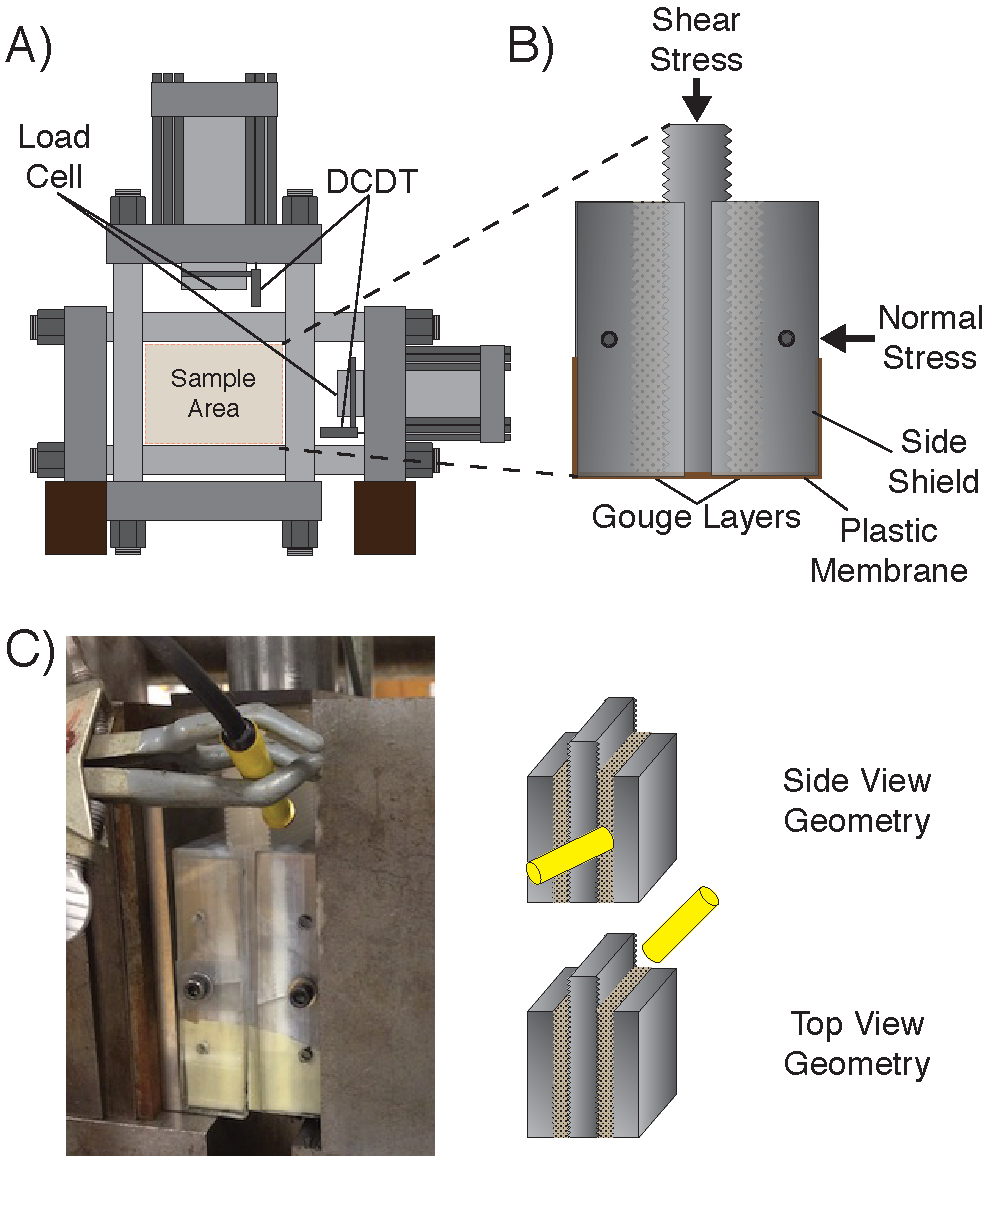
\includegraphics[width=30pc]{chap_electrical/biax_setup.pdf}
\caption{Experimental setup. A) The biaxial hydraulic press: sample assemblies are supported by steel blocks in the sample area. B) Double direct shear geometry consists of two layers of gouge confined between three forcing blocks.  Side shields and a plastic membrane are used to contain gouge material as the sample is sheared. C) Placement of the electrostatic voltmeter (yellow cylinder) in the side and top view positions.  A window was cut into the side shield for the side view geometry. }
\label{biax_setup}
\end{figure}

%% ---------------------------------- %%
%  Beads SEM Figure
%% ---------------------------------- %%
\begin{figure}
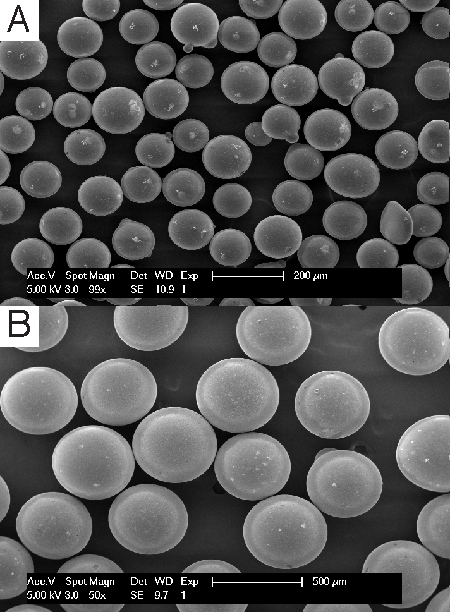
\includegraphics[width=30pc]{chap_electrical/sem_initial.pdf}
\caption{Scanning electron microscope micrographs of the starting glass beads for all experiments.  A) 100-150 $\mu m$ B) 420-500 $\mu m$}
\label{starting_SEM}
\end{figure}

%% ---------------------------------- %%
%  stick-slip Humidity
%% ---------------------------------- %%
\begin{figure}
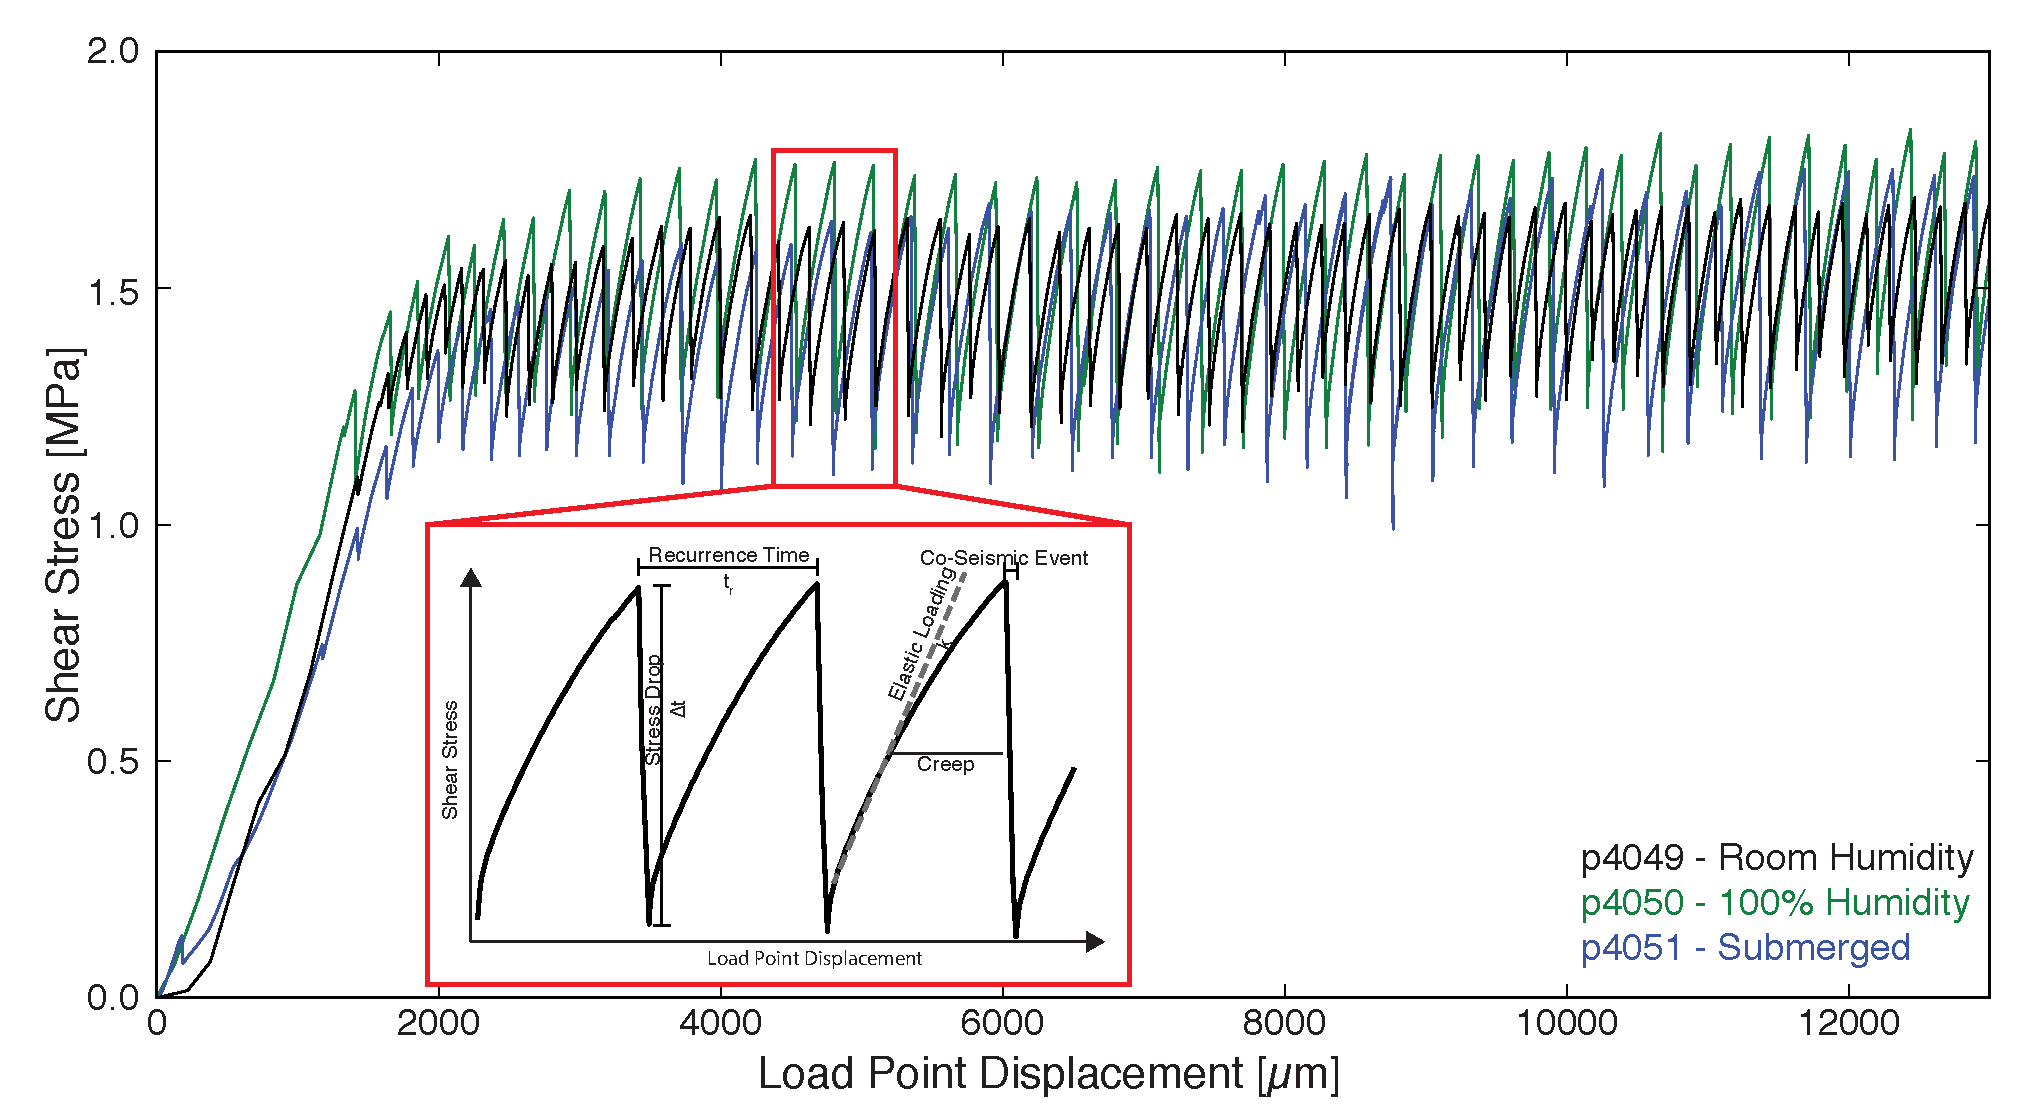
\includegraphics[width=40pc]{chap_electrical/ss_humidity.pdf}
\caption{Experiments performed on glass beads (100-150$\mu m$ diameter) under ambient humidity, 100\% humidity, and submerged conditions exhibit similar mechanical behavior.  Increased stress drops are observed with increased humidity and in the submerged case.  Inset: Anatomy of a stick-slip event.  The recurrence time is the time between peaks in shear stress.  Initially the shear stress increases linear-elastically.  Deviation from line-elastic behavior marks the onset of elasto-plastic deformation and pre-seismic slip.  When the ultimate strength of the layer is reached shear stress drops rapidly and the cycle begins again.}
\label{ss_humidity}
\end{figure}

%% ---------------------------------- %%
%  stick-slip Props
%% ---------------------------------- %%
\begin{figure}
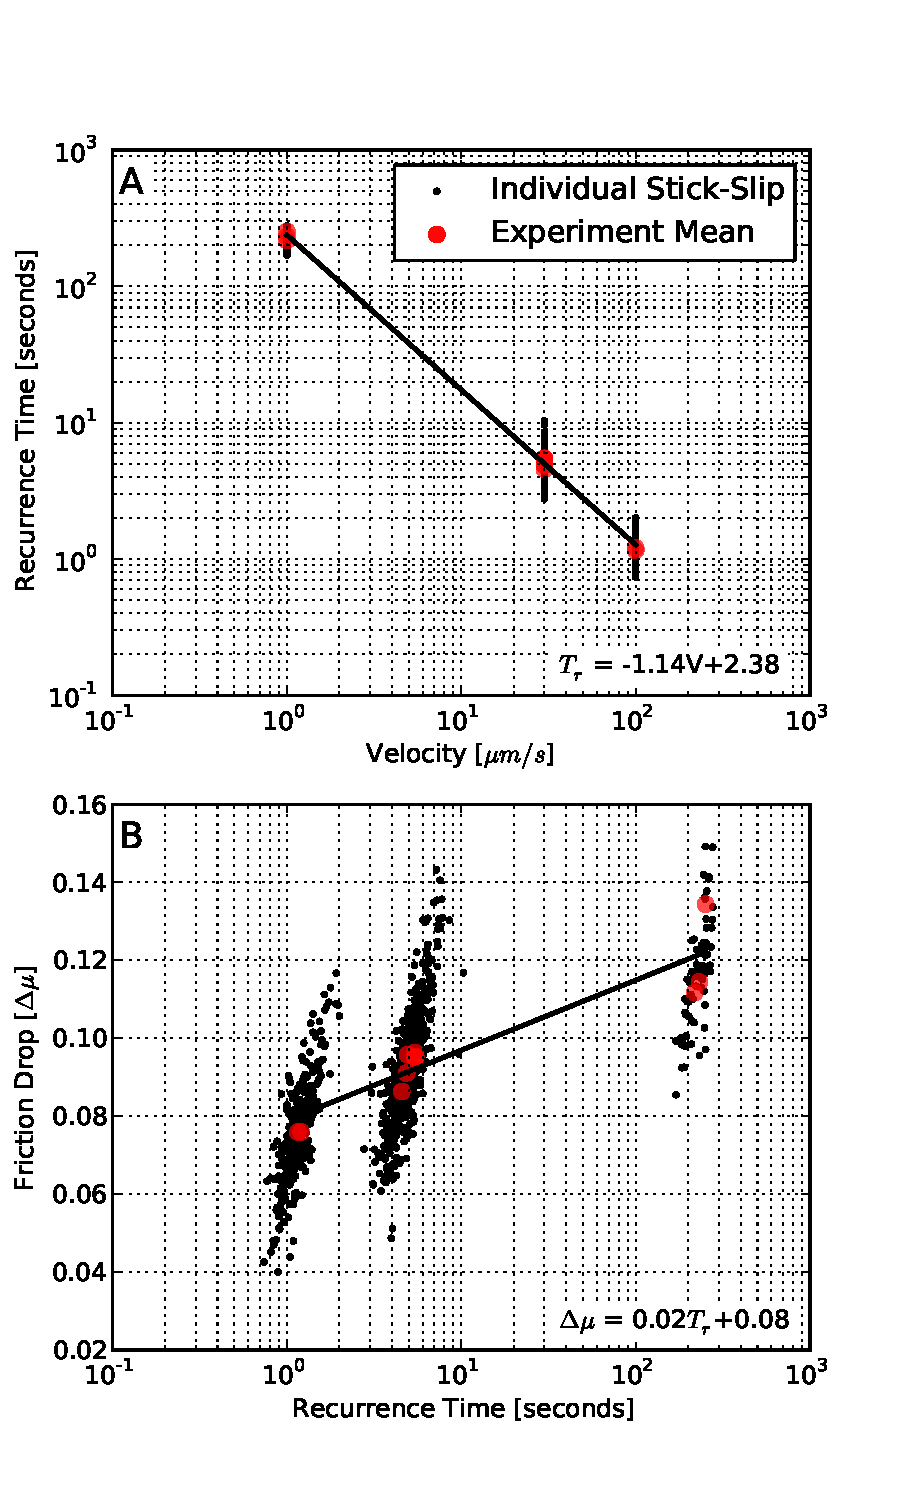
\includegraphics[width=25pc]{chap_electrical/ss_props.pdf}
\caption{A) Samples exhibit a log-log linear relation between recurrence time and velocity.  Faster loading rates result in shorter recurrence times. B) Friction drop increases with the recurrence time as there is more time for the layer to heal before the next stick-slip event.}
\label{ss_props}
\end{figure}

%% ---------------------------------- %%
%  Electrical Runplot
%% ---------------------------------- %%
\begin{figure}
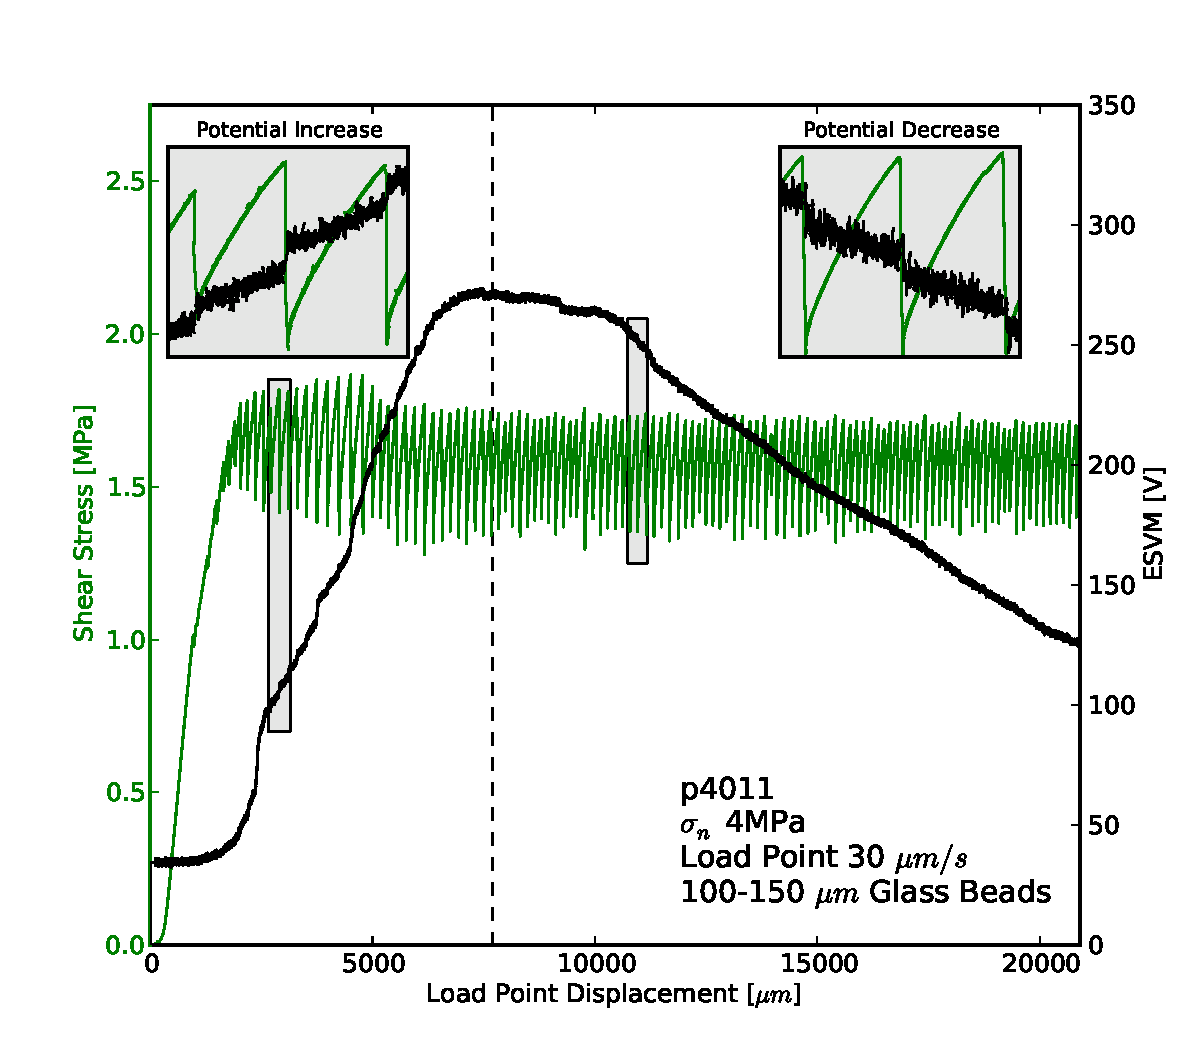
\includegraphics[width=40pc]{chap_electrical/elec_runplot.pdf}
\caption{During shearing two trends are observed: 1) A long-term charging/discharging trend in the electrical potential and 2) Potential change related to individual stick-slip events. The entire system initially charges, approximately until mechanical steady-state is reached. During this phase co-seismic potential changes are dominantly positive (top left inset).  After attainment of mechanical steady-state, the system begins to maintain or discharge potential.  During this phase the co-seismic potential changes are dominantly negative (top right inset).}
\label{electrical_runplot}
\end{figure}

%% ---------------------------------- %%
%  Electrical Zooms
%% ---------------------------------- %%
\begin{figure}
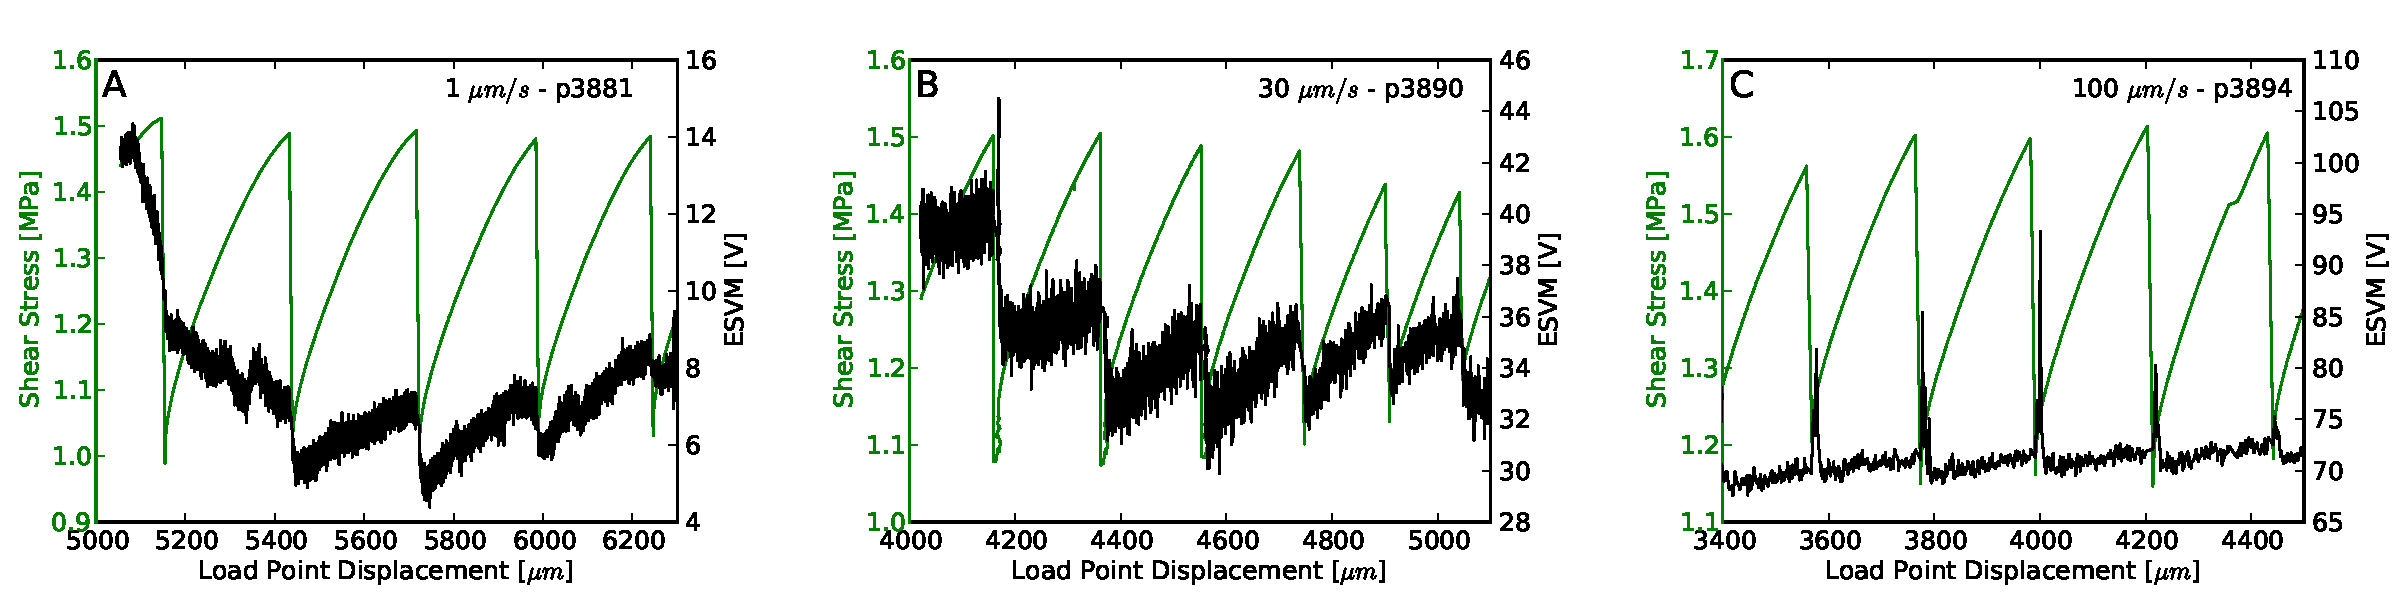
\includegraphics[width=45pc]{chap_electrical/elec_zooms.pdf}
\caption{Stick-slip events and associated ESVM measurements for three-different load point velocities of 1, 30, and 100 $\mu m/s$.  A) At slow loading velocities the electrical signal clearly mirrors the stress curve in most cases  B) For intermediate velocities, the relation is still present. C) At high velocities, the electrical signal is a sharp pulse an order of magnitude higher than those observed at low velocities, and we observe small inter-seismic charging.}
\label{electrical_zooms}
\end{figure}

%% ---------------------------------- %%
%  Voltage Change vs. Velocity log log
%% ---------------------------------- %%
\begin{figure}
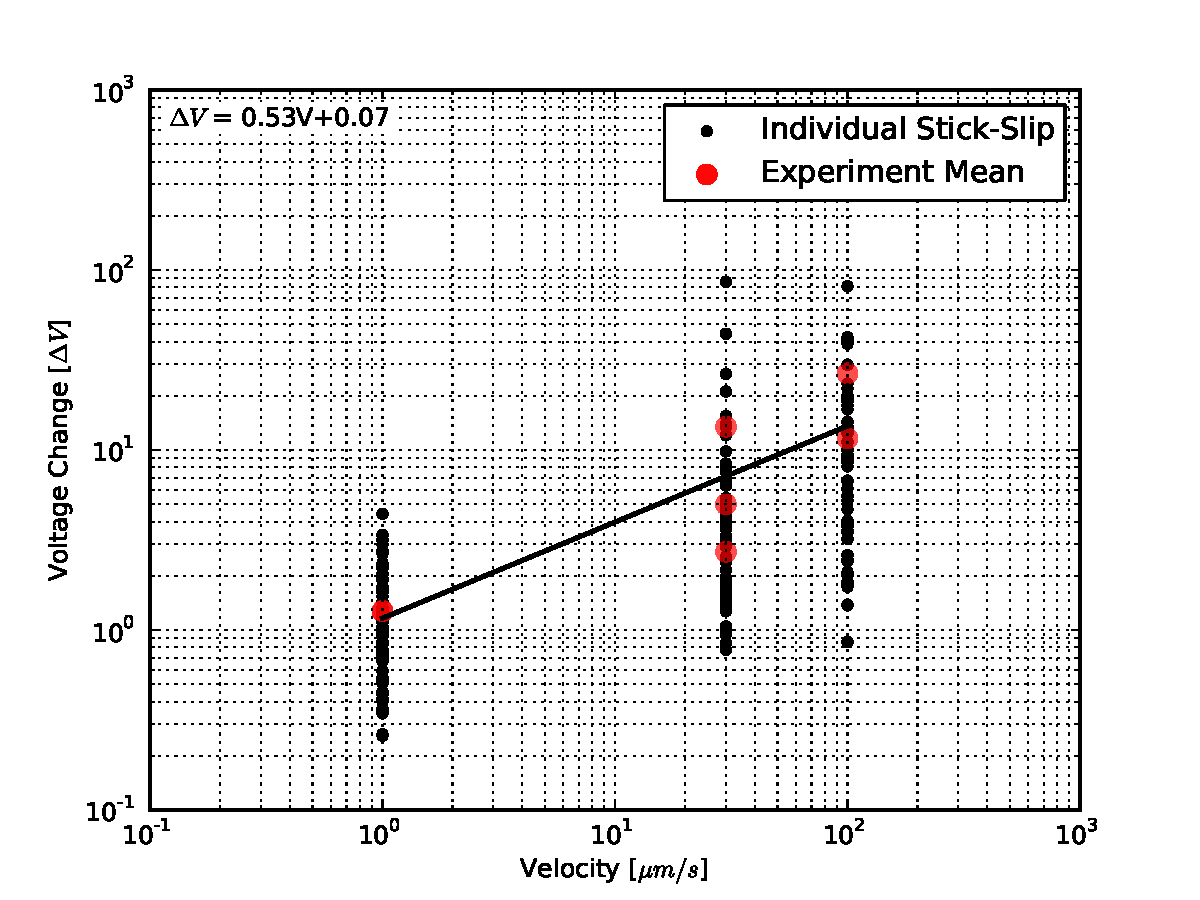
\includegraphics[width=30pc]{chap_electrical/vchange_velocity.pdf}
\caption{Each order of magnitude driving velocity change produces a $\sim$5x increase in the electrical signal observed.  All experiments shown are with the side-view sensor geometry.}
\label{voltage_velocity}
\end{figure}

%% ---------------------------------- %%
%  Model Cartoon
%% ---------------------------------- %%
\begin{figure}
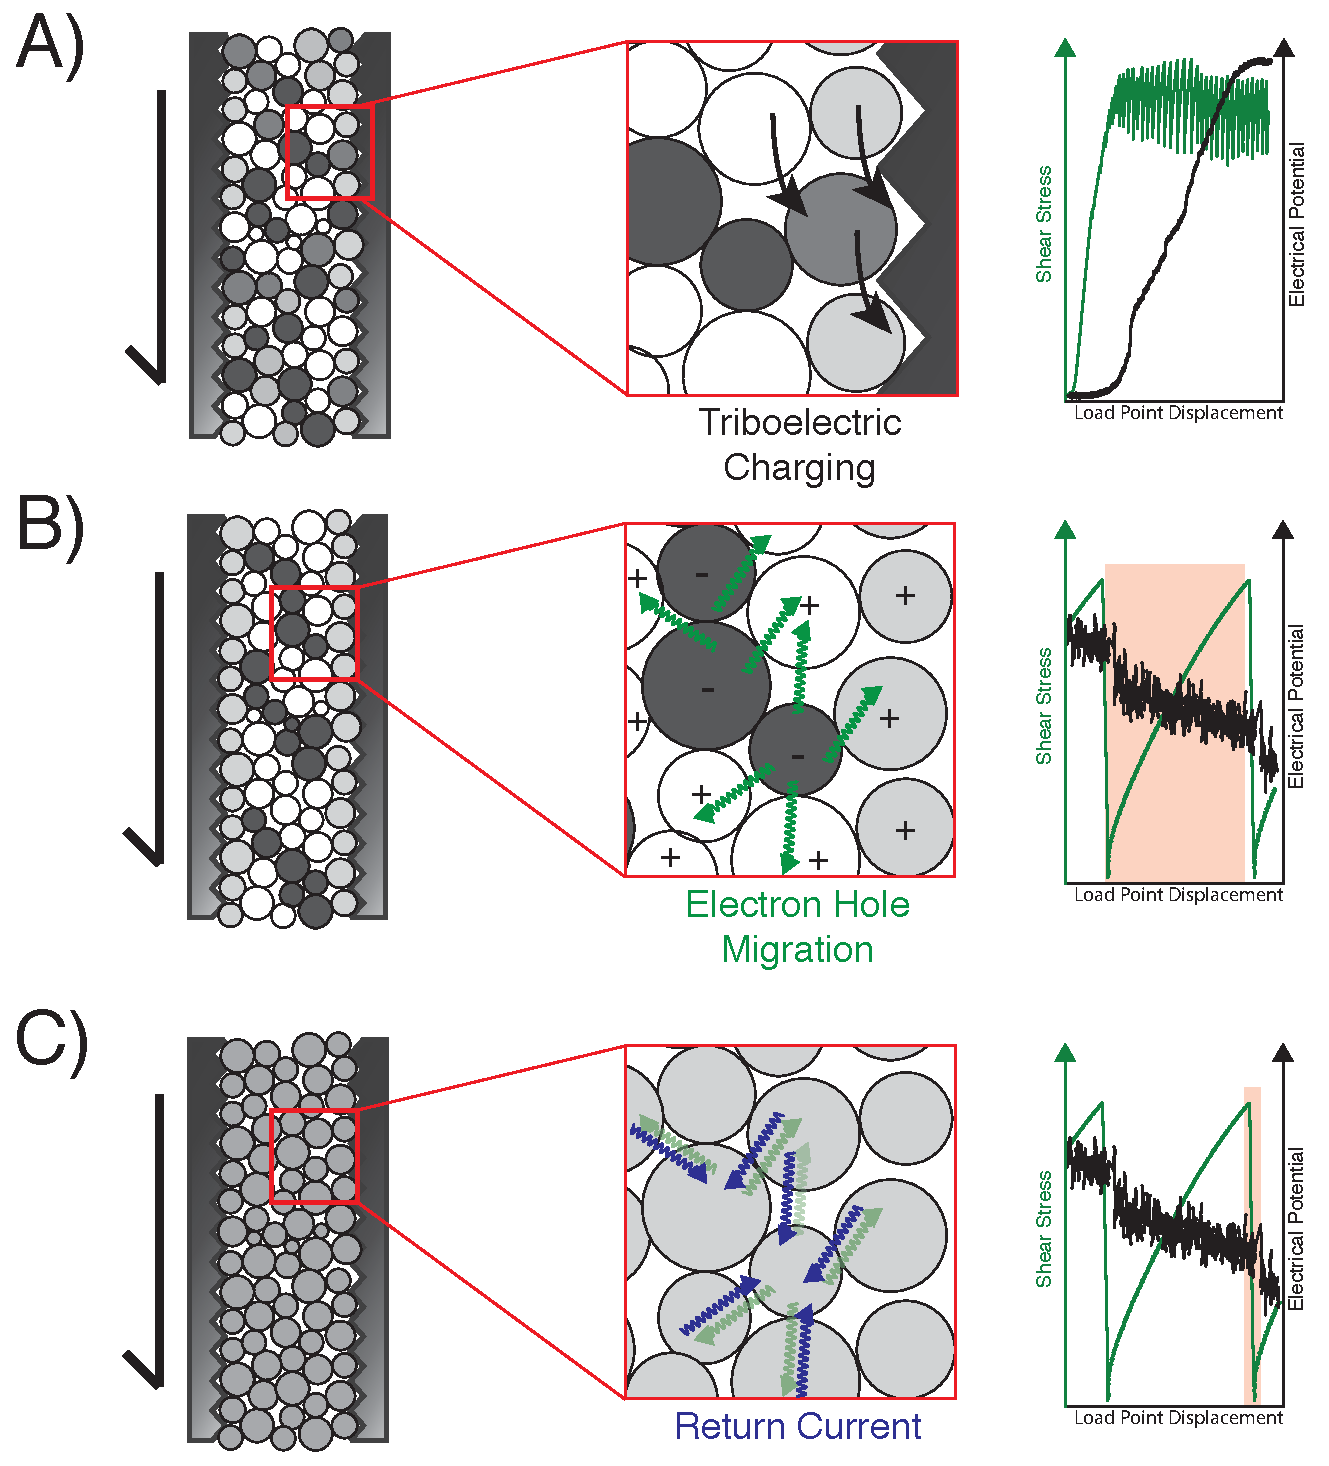
\includegraphics[width=30pc]{chap_electrical/model_cartoon.pdf}
\caption{A schematic representation of the stages of electrical behavior during an experiment:  A) During the initial run-in there is massive grain rearrangement as force chain networks begin to form.  This sliding motion tribo-electrically charges the system.  B) After the force chain network forms there is minimal grain-boundary sliding.  Shear loads are supported in the granular layer by highly stressed force chains (dark colors).  Electron holes migrate away from highly stressed beads into the matrix creating an electrical potential gradient.  C) When the layer fails and all grains are at roughly the same low stress, a return current redistributes the electrical gradient and the cycle begins again.}
\label{model_cartoon}
\end{figure}

%% ---------------------------------- %%
%  Appendix A - ESVM Calibration
%% ---------------------------------- %%
\begin{figure}
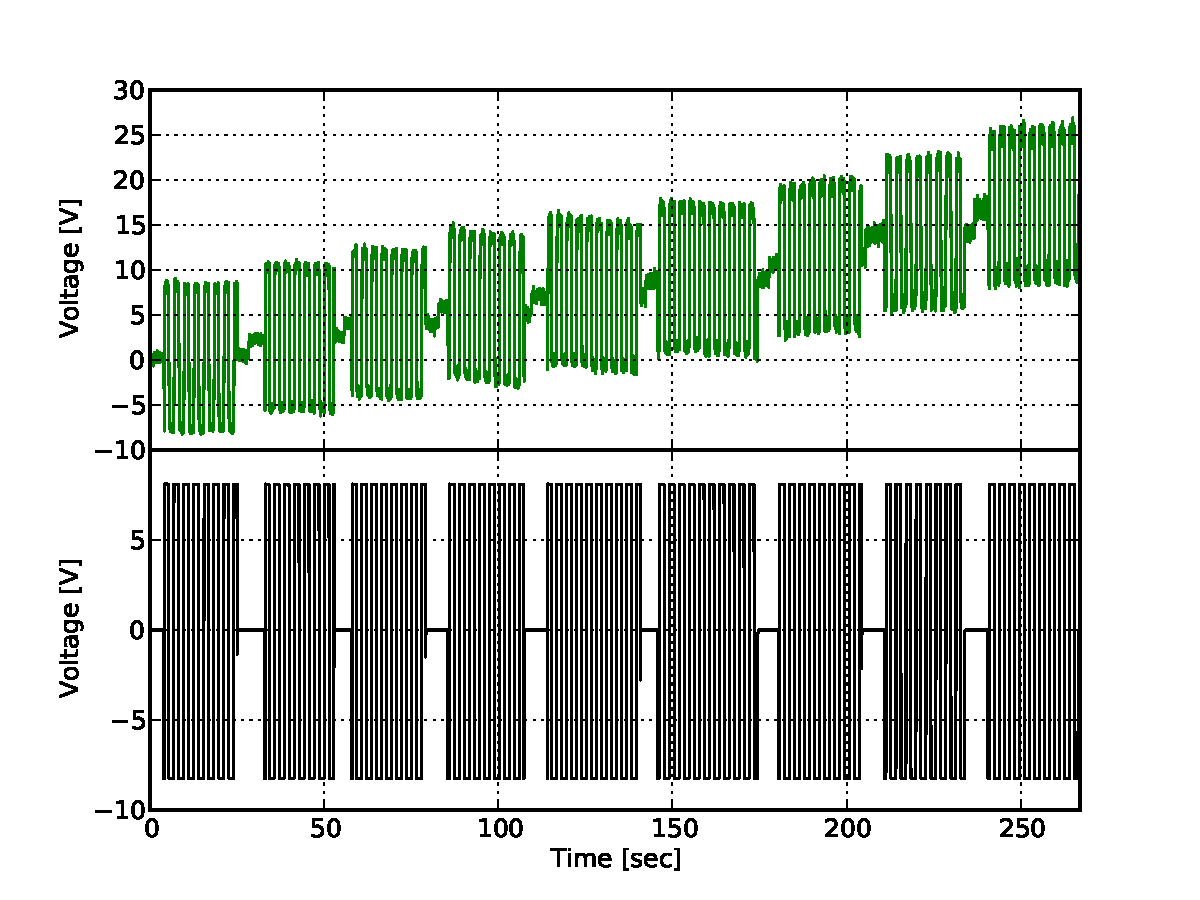
\includegraphics[width=30pc]{chap_electrical/ESVM_Calibration.pdf}
\caption{Calibration of the ESVM from a function generator source (bottom panel).  A series of steps through the ESVM `response' setting from 1-9 shows that the input square wave applied to the aluminium surface under test is well-recorded on each setting (top panel).  The upward trend in ESVM data is a product of a DC offset that occurs each time the response setting is changed on the instrument.}
\label{esvm_calibration}
\end{figure}

%% ---------------------------------- %%
%  Appendix A - ESVM response
%% ---------------------------------- %%
\begin{figure}
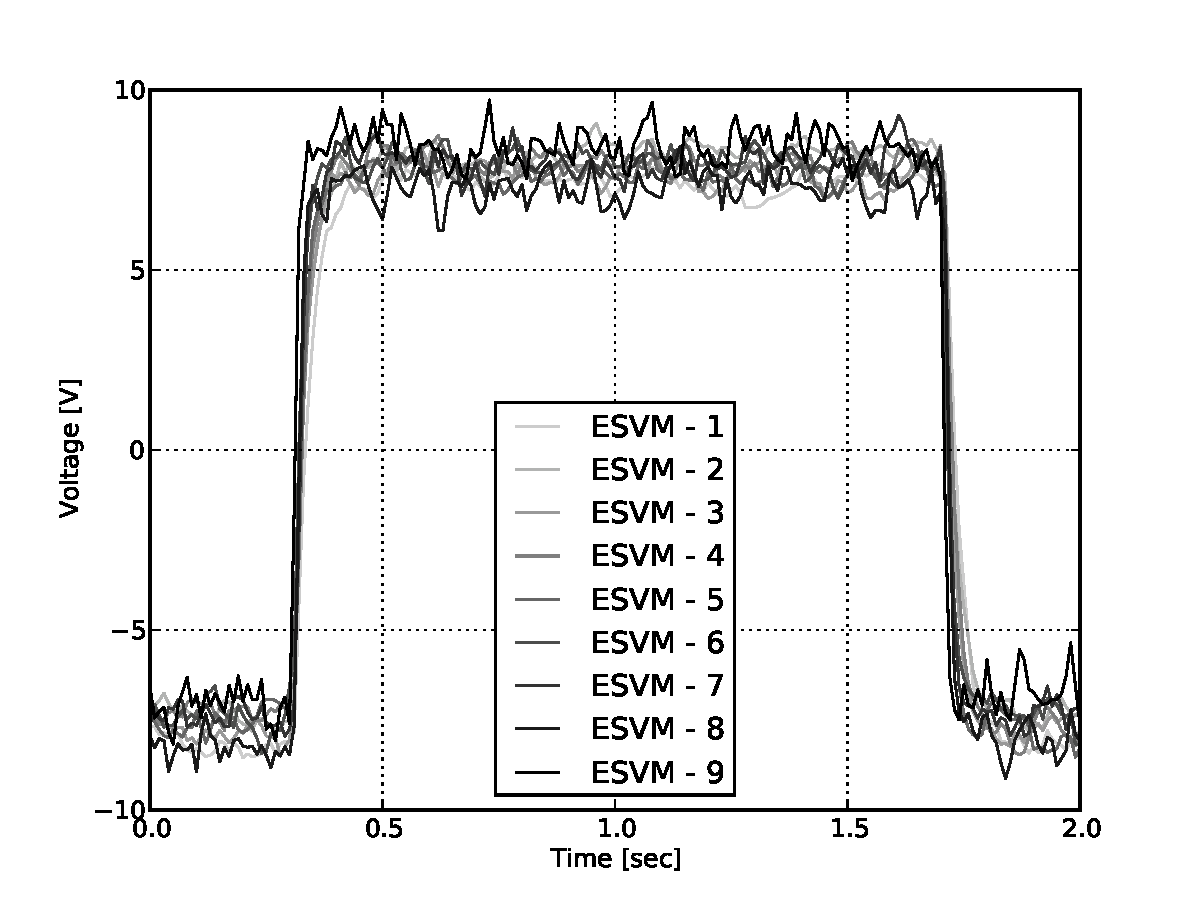
\includegraphics[width=30pc]{chap_electrical/ESVM_Calibration_Pulse.pdf}
\caption{A detailed comparison of a single waveform shows that at lower response settings (lighter colors) the waveform is smoothed slightly, with the nearly instantaneous voltage change distributed over up to 0.1 seconds on both the rise and fall.  At higher resolutions (darker colors) the sharp transition is clearly seen, but at the price of a higher noise level during the flat hold states.}
\label{esvm_response}
\end{figure}

%% ---------------------------------- %%
%  Appendix A - ESVM response timing
%% ---------------------------------- %%
\begin{figure}
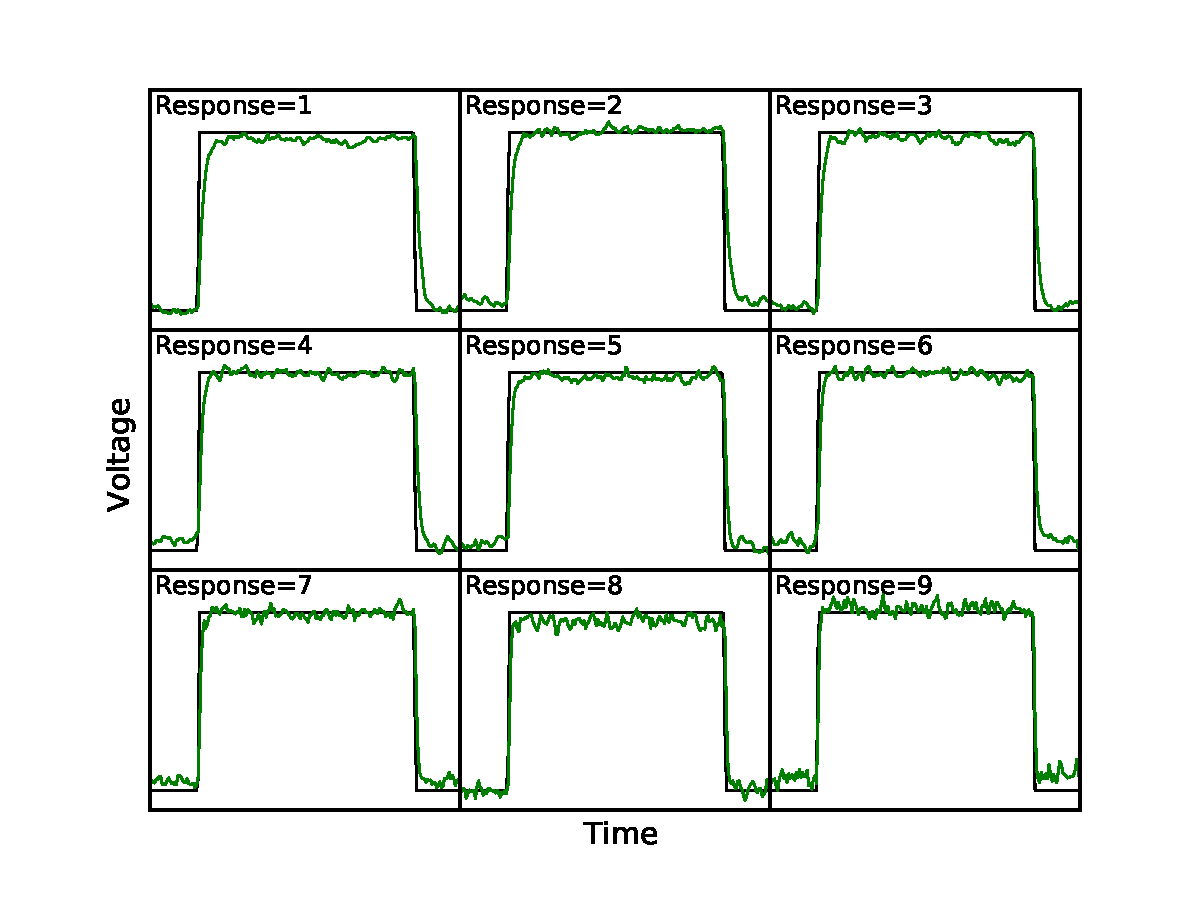
\includegraphics[width=30pc]{chap_electrical/ESVM_Allchan_timing.pdf}
\caption{At all response settings the beginning of ESVM signal change corresponds well in the time domain with the leading and falling edge of the input signal.  Smoothing due to longer integration times is observed at low response settings.}
\label{esvm_timing}
\end{figure}

%% ---------------------------------- %%
%  Table of Experiments
%% ---------------------------------- %%
\begin{table}
\caption{List of Experiments}
\centering
\begin{tabular}{c c c c c c}
\hline
 Experiment & $V_{lp}$, $\mu m/s$ & Bead Size, $\mu m$ & Temperature, $C^\circ$& Humidity, \%& Comment \\
\hline
p3853 & 30   & 420-500 & 23.3 & 41.2 & Large Beads\\
p3878 & 30   & 100-150 & 23.8 & 23.8 & Side View\\
p3879 & 30   & 420-500 & 24.7 & 20.2 & Large Beads\\
p3880 & 30   & 420-500 & 25.7 & 20.7 & Large Beads\\
p3881 & 30   & 100-150 & 26.9 & 20.7 & Side View\\
p3882 & 30   & 100-150 & 26.0 & 14.0 & Side View\\
p3887 & 30   & 100-150 & 22.7 & 22.5 & Side View\\
p3889 & 1     & 100-150 & 23.4 & 24.8 & Side View\\
p3890 & 100 & 100-150 & 24.1 & 33.8 & Side View\\
p3893 & 100 & 100-150 & 21.9 & 19.9 & Side View\\
p3894 & 1     & 100-150 & 22.7 & 19.8 & Side View\\
p4010 & 30   & 100-150 & 23.9 & 23.0 & Top View - Isolated Ground\\
p4011 & 30   & 100-150 & 24.2 & 23.7 & Top View\\
p4012 & 30   & 100-150 & 24.5 & 22.0 & Top View\\
p4013 & 1     & 100-150 & 24.3 & 22.3 & Top View\\
p4014 & 30   & 100-150 & 23.0 & 100  & Saturated\\
p4015 & 30   & 100-150 & 23.3 & N/A  & Submerged\\
p4049 & 30   & 100-150 & 23.9 & 27.0 & Control Test \\
p4050 & 30   & 100-150 & 23.8 & 100  & Saturated \\
p4051 & 30   & 100-150 & 23.9 & N/A  & Submerged \\
p4052 & 30   & 100-150 & 23.8 & 100  & Saturated \\
\hline
\label{exp_list}
\end{tabular}
\end{table}


%% ---------------------------------- %%
%  Table of Bead Composition
%% ---------------------------------- %%
\begin{table}
\caption{Composition of glass beads.}
\centering
\begin{tabular}{c c}
\hline
Compound & Composition,\%\\
\hline
SiO$_2$ & 65-75\% \\
Al$_2$O$_3$ & 0-5\%\\
CaO & 6-15\% \\
MgO & 1-5\%\\
Na$_2$O & 10-20\%\\
Fe$_2$O$_3$ & \textless 0.8\%\\
\hline
\label{bead_composition}
\end{tabular}
\end{table}

%\begin{singlespace}
%\include{conclusions}

%% now we include the appendices
\appendices
%% omit this if there are no appendices

%% if there is only one appendix, 
%% say \singleappendix instead of \appendices
% \singleappendix

%% these are the actual commands to include the apendix files:
\addcontentsline{toc}{chapter}{Appendix A. List of Biaxial Experiments}  
\chapter{List of Biaxial Experiments}

% Please add the following required packages to your document preamble:
% \usepackage[normalem]{ulem}
% \useunder{\uline}{\ul}{}
%\begin{longtable}[]
%\centering
%\caption{My caption}
%\label{my-label}
\setlength\LTleft{0pt}
\setlength\LTright{0pt}
\begin{landscape}
\tiny
\begin{longtable} {lllllllllllllll}
Date     & Exp. & Block            & Material     & Grain Size   & Thickness & $\sigma_n$ & Velocity                     & Temperature & Humidity & Purpose\\
Text     & Num        & Material         & Text         & um           & mm        & MPa           & $\mu\text{m/s}$                         & C           & \%       & Text \\
\hline
\hline
8/31/12  & p3805      & Granite          & Glass Beads  & 100-150      & 5         & 5             & 5                           & 24          & 57.4     & ESVM\\
9/3/12   & p3809      & Granite          & Glass Beads  & 100-150      & 5         & 5             & 10                           & 24          & 80       & ESVM\\
9/21/12  & p3825      & Granite          & Glass Beads  & 100-150      & 5         & 1             & 10                           & -           & -        & ESVM\\
9/22/12  & p3826      & Granite          & Glass Beads  & 100-150      & 5         & 31            & 10                           & 23.4        & 65       & ESVM\\
9/22/12  & p3827      & Steel            & Glass Beads  & 100-150      & 5         & 2.5,4         & 1,10                      & 23.1        & 63       & ESVM\\
9/23/12  & p3828      & Steel            & Glass Beads  & 100-150      & 5         & 2.5,4         & 10                           & 22.8        & 39.9     & ESVM\\
9/23/12  & p3829      & Steel            & Glass Beads  & 100-150      & 5         & 10            & 10                           & 23.5        & 38.1     & ESVM\\
9/24/12  & p3830      & Steel            & Glass Beads  & 100-150      & 5         & 10            & 10-500 & 21.9        & 41       & ESVM\\
9/24/12  & p3831      & Steel            & Glass Beads  & 100-150      & 5         & 10            & 10-100                 & 22.3        & 16       & Low RH ESVM\\
10/18/12 & p3846      & Acry/UMHW        & Glass Beads  & 100-150      & 5         & 0.5,1         & N/A                          & 25.8        & 33       & Test New Blocks\\
10/29/12 & p3851      & Acry          & Glass Beads  & 100-150      & 5         & 4.3           & 10-100                    & 22.4        & 44       & ESVM\\
10/29/12 & p3852      & Acry          & Glass Beads  & 420-500      & 5         & 4.3           & 10-100             & 22.7        & 42.9     & ESVM\\
10/29/12 & p3853      & Acry          & Glass Beads  & 420-500      & 5         & 4.3           & 30                           & 23.3        & 41.2     & ESVM\\
11/13/12 & p3878      & Acry          & Glass Beads  & 100-150      & 5         & 4             & 30                           & 23.8        & 23.8     & ESVM\\
11/14/12 & p3879      & Acry          & Glass Beads  & 420-500      & 5         & 4             & 30                           & 24.7        & 20.2     & ESVM\\
11/14/12 & p3880      & Acry          & Glass Beads  & 420-500      & 5         & 4             & 30                           & 25.7        & 20.7     & ESVM\\
11/15/12 & p3881      & Acry          & Glass Beads  & 100-150      & 5         & 4             & 30                           & 26.9        & 20.7     & ESVM\\
11/16/12 & p3882      & Acry          & Glass Beads  & 100-150      & 5         & 4             & 30                           & 26          & 14       & Low RH ESVM\\
11/22/12 & p3886      & Ice Core         & Ice          & N/A          & N/A       & N/A           & 100                          & 21.6        & 26.9     & Signal from Ice\\
11/22/12 & p3887      & Acry          & Glass Beads  & 100-150      & 5         & 4             & 30                           & 22.7        & 22.5     & ESVM\\
11/22/12 & p3888      & Acry          & Glass Beads  & Mixed        & 7         & 4             & 10                           & 22.7        & 24.7     & Video\\
11/23/12 & p3889      & Acry          & Glass Beads  & 100-150      & 5         & 4             & 1                            & 23.4        & 24.8     & ESVM\\
11/23/12 & p3890      & Acry          & Glass Beads  & 100-150      & 5         & 4             & 100                          & 24.1        & 33.8     & ESVM\\
11/23/12 & p3891      & Ice Core         & Ice          & N/A          & N/A       & N/A           & 100                          & 23.8        & 30.4     & Signal from Ice\\
11/23/12 & p3892      & Acry          & Glass Beads  & Mixed        & 7         & 4             & 10                           & 23.3        & 28.7     & Video of beads\\
11/24/12 & p3893      & Acry          & Glass Beads  & 100-150      & 5         & 4             & 100                          & 21.9        & 19.9     & ESVM\\
11/24/12 & p3894      & Acry          & Glass Beads  & 100-150      & 5         & 4             & 1                            & 22.7        & 19.8     & ESVM\\
11/24/12 & p3895      & Ice Core         & Ice          & N/A          & N/A       & N/A           & 100                          & 22.5        & 20.1     & Signal from Ice\\
12/13/12 & p3916      & Acry          & Flour        & Unknown      & 7         & 1             & 0.1-100     & 23.5        & 22       & Flour Props.\\
12/14/12 & p3917      & Acry/Steel    & Flour        & Unknown      & 7         & 1             & 0.1-10                     & 22          & 21.9     & Flour Vel.\\
12/15/12 & p3918      & Acry          & Flour        & Unknown      & 7         & 1             & 10,1                         & 23.1        & 22       & Flour ESVM\\
12/15/12 & p3919      & Acry          & Flour        & Unknown      & 7         & 1             & 1                            & 24.2        & 23.9     & Flour ESVM\\
12/15/12 & p3920      & Acry          & Flour        & Unknown      & 7         & 1             & 1,10                         & 24.4        & 25       & Flour ESVM\\
3/13/13  & p4010      & Acry          & Glass Beads  & 100-150      & 5         & 4             & 30                           & 23.9        & 23       & Top View - not gnded\\
3/13/13  & p4011      & Acry          & Glass Beads  & 100-150      & 5         & 4             & 30                           & 24.2        & 23.7     & Top View - gnded\\
3/13/13  & p4012      & Acry          & Glass Beads  & 100-150      & 5         & 4             & 30                           & 24.5        & 22       & Top View\\
3/13/13  & p4013      & Acry          & Glass Beads  & 100-150      & 5         & 4             & 1                            & 24.3        & 22.3     & Top View\\
3/14/13  & p4014      & Acry          & Glass Beads  & 100-150      & 5         & 4             & 30                           & 23          & 100      & High RH\\
3/14/13  & p4015      & Acry          & Glass Beads  & 100-150      & 5         & 4             & 30                           & 23.3        & N/A      & Submerged\\
4/13/13  & p4049      & Acry          & Glass Beads  & 100-150      & 5         & 4             & 30                           & 23.9        & 27       & ESVM Control\\
4/14/13  & p4050      & Acry          & Glass Beads  & 100-150      & 5         & 4             & 30                           & 23.8        & 100      & High RH\\
4/14/13  & p4051      & Acry          & Glass Beads  & 100-150      & 5         & 4             & 30                           & 23.9        & N/A      & Submerged\\
4/15/13  & p4052      & Acry          & Glass Beads  & 100-150      & 5         & 4             & 30                           & 23.8        & 100      & High RH\\
5/5/13   & p4061      & N/A              & Granite Core & N/A          & N/A       & N/A           & N/A                          & -           & -        & P4000 Celebration\\
5/26/13  & p4071      & Steel/Acry    & F110         & -            & 3         & 2             & various                      & 23.3        & 30.1     & Stable or SS\\
5/26/13  & p4072      & Steel/UMHW       & F111         & -            & 3         & 2             & various                      & 23.4        & 25.4     & Stable or SS\\
5/27/13  & p4073      & Steel            & Flour        & -            & 8         & 1             & various                      & 23.4        & 28.4     & Stable or SS\\
5/27/13  & p4074      & Steel/Acry    & Flour        & -            & 8         & 1             & various                      & 23.1        & 38.8     & Stable or SS\\
6/28/13  & p4080      & Large Steel      & N/A          & N/A          & N/A       & N/A           & 5                            & 24.1        & 66.4     & Horiz k\\
6/28/13  & p4081      & Large Steel      & N/A          & N/A          & N/A       & N/A           & 5                            & 24.2        & 65.9     & Vert k\\
6/28/13  & p4082      & Large Steel      & N/A          & N/A          & N/A       & N/A           & 5                            & 24.2        & 64.6     & Poisson\\
6/28/13  & p4083      & Large Steel      & N/A          & N/A          & N/A       & N/A           & 5                            & 24.4        & 64.6     & Horiz k\\
6/28/13  & p4084      & Large Steel      & N/A          & N/A          & N/A       & N/A           & 5                            & 24.6        & 64.1     & Vert k\\
6/28/13  & p4085      & Large Steel      & N/A          & N/A          & N/A       & N/A           & 5                            & 24.6        & 63.9     & Poisson\\
7/1/13   & p4086      & Large Steel      & N/A          & N/A          & N/A       & N/A           & 5                            & 24.1        & 68.4     & Horiz k\\
7/1/13   & p4087      & Large Steel      & N/A          & N/A          & N/A       & N/A           & 5                            & 23.9        & 68       & Vert k\\
7/1/13   & p4088      & Large Steel      & N/A          & N/A          & N/A       & N/A           & 5                            & 23.9        & 67.5     & Poisson\\
7/22/13  & p4108      & Granite          & N/A          & N/A          & N/A       & 2             & various                      & 25.5        & 58.5     & Acou - Vel steps\\
7/25/13  & p4111      & Granite          & N/A          & N/A          & N/A       & 2             & various                      & 25.2        & 49.2     & Acou - Vel steps\\
7/26/13  & p4112      & Steel            & Flour        & Unknown      & 8         & 1             & various                      & 24.3        & 55.5     & SHS\\
7/26/13  & p4113      & Steel            & Flour        & Unknown      & 8         & 1             & various                      & 24.3        & 56.1     & SHS/Steps\\
7/30/13  & p4115      & Granite          & N/A          & N/A          & N/A       & 4             & various                      & 24.5        & 55.5     & Acou - Vel steps\\
7/30/13  & p4116      & Granite          & N/A          & N/A          & N/A       & 4             & various                      & N/A         & N/A      & Acou - Vel steps\\
7/30/13  & p4117      & Granite          & N/A          & N/A          & N/A       & 4             & various                      & 24.7        & 54.7     & Acou - Vel steps\\
7/31/13  & p4118      & Granite          & N/A          & N/A          & N/A       & 4             & various                      & 24.3        & 57.5     & Acou - Vel steps/SHS\\
7/31/13  & p4119      & Granite          & N/A          & N/A          & N/A       & 4             & various                      & 24.5        & 56.1     & Acou - Rubin/SHS\\
8/1/13   & p4120      & Granite          & N/A          & N/A          & N/A       & 4             & various                      & 24.4        & 60.3     & Acou - Rubin/SHS\\
8/2/13   & p4121      & Steel            & F110         & N/A          & 5         & 25            & various                      & 24.7        & 556.6    & Acou - Rubin/V steps\\
11/9/13  & p4175      & steel            & F110         & N/A          & 5         & 25            & 10                           & 24.3        & 24.1     & Dry and submerged\\
11/10/13 & p4176      & steel            & Alpine Fault & \textless125 & 5         & 30            & 10                           & 23          & 19       & SHS\\
11/10/13 & p4177      & steel            & Alpine Fault & \textless125 & 5         & 30            & 10                           & 23.6        & 26.5     & SHS\\
11/10/13 & p4178      & steel            & Alpine Fault & \textless125 & 5         & 30            & 10                           & 23.8        & 22.5     & SHS\\
11/15/13 & p4181      & Steel            & Glass Beads  & 100-150      & 5         & 4.5           & various                      & 24.7        & 19.5     & PJ - Acou\\
11/15/13 & p4182      & Steel            & Glass Beads  & 100-150      & 5         & 4.5           & various                      & 24.6        & 21       & PJ - Acou\\
11/16/13 & p4183      & Steel            & Glass Beads  & 100-150      & 5         & 4.5           & various                      & 25.4        & 28.6     & PJ - Acou\\
11/16/13 & p4184      & Steel/UMHW       & Min-u-sil    & 10           & 3         & 1             & various                      & 26          & 30.2     & PJ - Stiffness\\
11/16/13 & p4185      & Ti/Acry & Min-u-sil    & 10           & 3         & 4             & various                      & 24.3        & 33       & PJ - Stiffness\\
11/17/13 & p4186      & Ti/Acry & Min-u-sil    & 10           & 3         & 4             & various                      & 23.9        & 42.7     & PJ - Stiffness\\
11/17/13 & p4187      & Ti/Acry & Min-u-sil    & 10           & 3         & 4             & various                      & 25.5        & 42.2     & PJ - Stiffness\\
11/17/13 & p4188      & Steel/Acry    & Westerly Po  & \textless125 & 3         & 4             & various                      & 25          & 46.5     & PJ - Stiffness\\
11/17/13 & p4189      & Ti/Acry & Min-u-sil    & 10           & 3         & 4             & various                      & 26          & 45.3     & PJ - Stiffness\\
11/18/13 & p4190      & Granite          & N/A          & N/A          & N/A       & 3             & various                      & 24.3        & 34.1     & PJ - Stiffness\\
11/18/13 & p4191      & Ti/Acry & Min-u-sil    & 10           & 3         & 4             & various                      & 24.6        & 30.1     & PJ - Stiffness\\
1/10/14  & p4206      & Steel/Acry    & Min-u-sil    & 10           & 3         & 4             & various                      & 23.3        & 22.4     & Slow-Slip\\
1/10/14  & p4207      & Steel/Acry    & Min-u-sil    & 10           & 3         & 4             & various                      & 23.2        & 23.3     & Slow-Slip\\
1/23/14  & p4211      & Steel            & F110         & 110          & 5         & 25            & various                      & 23.3        & 16       & Kerry 508 Project\\
11/18/13 & p4192      & Steel            & Min-u-sil    & 10           & 3         & 4             & various                      & 25.4        & 29.8     & PJ - Stiffness\\
2/27/13  & p4224      & Ti/Acry & Min-u-sil    & 10           & 3         & 5             & various                      & 26          & 16       & Test New Acry Block\\
2/28/14  & p4225      & Ti/Acry & Min-u-sil    & 10           & 3         & 5             & various                      & 22          & 16       & Old Acry Block\\
2/28/14  & p4226      & Ti/Acry & Min-u-sil    & 10           & 3         & 4             & various                      & 22          & 16       & Old Acry Block\\
3/1/14   & p4227      & Ti/Acry & Min-u-sil    & 10           & 3         & 4             & various                      & 24          & 100      & Old Acry Block\\
3/1/14   & p4228      & Steel            & Min-u-sil    & 10           & 3         & 4             & various                      & 24          & 100      & SHS\\
3/3/14   & p4229      & Ti/Acry & Min-u-sil    & 10           & 3         & 4             & various                      & 24          & 100      & New Acry\\
         & p4238      &                  &              &              &           &               &                              &             &          &                                                 \\
4/25/14  & p4247      & Ti/Acry & Min-u-sil    & 10           & 3         & 4             & various                      & 23          & 100      & New 5x5 Acry\\
4/26/14  & p4248      & Ti/Acry & Min-u-sil    & 10           & 3         & 4             & various                      & 24.2        & 100      & New Acry\\
4/26/14  & p4249      & Ti/Acry & Min-u-sil    & 10           & 3         & 4             & various                      & 23.2        & 100      & New Acry\\
4/27/14  & p4250      & Ti/Acry & Min-u-sil    & 10           & 3         & 4             & various                      & 22.7        & 100      & Old Acry\\
4/27/14  & p4251      & Ti/Acry & Min-u-sil    & 10           & 3         & 4             & various                      & 23.2        & 22       & Old Acry\\
5/22/14  & p4267      & Ti/Acry & Min-u-sil    & 10           & 3         & 2             & various                      & 23.2        & 100      & New Acry\\
5/23/14  & p4268      & Ti/Acry & Min-u-sil    & 10           & 3         & 8             & 10                           & 23.4        & 100      & New Acry\\
5/23/14  & p4269      & Steel            & Min-u-sil    & 10           & 3         & 4             & various                      & 23.4        & 100      & Steps\\
5/24/14  & p4270      & Steel            & Min-u-sil    & 10           & 3         & 2             & various                      &             & 100      & Steps\\
5/24/14  & p4271      & Ti/Acry & Min-u-sil    & 10           & 3         & 2             & various                      &             & 100      & Steps\\
5/25/14  & p4272      & Ti/Acry & Min-u-sil    & 10           & 3         & 8             & 10                           & 22.7        & 100      & New Acry\\
5/25/14  & p4273      & Steel            & Min-u-sil    & 10           & 3         & 8             & various                      & 23.4        & 100      & Steps\\
8/28/14  & p4308      & Steel            & N/A          & N/A          & N/A       & 4             & N/A                          & 23.5        & 57       & P/S wave block\\
8/31/14  & p4309      & Steel            & Min-u-sil    & 10           & 3         & 8             & various                      & 23.2        & 100      & RSF\\
8/31/14  & p4310      & Ti/Acry & Min-u-sil    & 10           & 3         & 8             & various                      & 24.2        & 100      & Fine Acry\\
9/1/14   & p4311      & Ti/Acry & Min-u-sil    & 10           & 3         & 8             & various                      & 23.3        & 100      & Thick Acry\\
9/1/14   & p4312      & Steel/Acry    & Min-u-sil    & 10           & 3         & 8             & various                      & 23.6        & 100      & Thick Acry\\
9/2/14   & p4313      & Ti/Acry & Min-u-sil    & 10           & 3         & 8             & various                      & 23.5        & 100      & Fine Acry\\
9/2/14   & p4314      & Steel            & Min-u-sil    & 10           & 3         & 12            & various                      & 24.3        & 100      & RSF\\
9/2/14   & p4315      & N/A              & N/A          & N/A          & N/A       & N/A           & N/A                          & N/A         & N/A      & Block k\\
9/3/14   & p4316      & Ti/Acry & Min-u-sil    & 10           & 3         & 12            & various                      & 23.6        & 100      & Fine Acry\\
9/3/14   & p4317      & Steel/Acry    & Min-u-sil    & 10           & 3         & 12            & various                      & 24.2        & 100      & Fine Acry\\
10/11/14 & p4327      & Steel            & Min-u-sil    & 10           & 3         & 6             & various                      & 22.5        & 100      & RSF\\
10/11/14 & p4328      & Ti/Acry & Min-u-sil    & 10           & 3         & 6             & various                      & 22.7        & 100      & Fine Acry\\
10/12/14 & p4329      & Ti/Acry & Min-u-sil    & 10           & 3         & 6             & various                      & 22          & 100      & Fine Acry\\
10/12/14 & p4330      & Steel            & Min-u-sil    & 10           & 3         & 6             & various                      & 22.9        & 100      & RSF\\
11/3/14  & p4336      & Ti/Acry & Min-u-sil    & 10           & 3         & 8             & 10                           & 24.8        & 100      & Vp Slow Slip\\
11/4/14  & p4337      & Ti/Acry & Min-u-sil    & 10           & 3         & 8             & 10                           & 24.8        & 100      & Vs Slow Slip\\
11/15/14 & p4338      & Ti/Acry & Min-u-sil    & 10           & 3         & 4             & 10                           & 24.2        & 100      & Unload/reload k\\
11/15/14 & p4339      & Steel            & Min-u-sil    & 10           & 3         & 4             & various                      & 24.8        & 100      & Unload/reload, RSF\\
11/16/14 & p4340      & Ti/Acry & Min-u-sil    & 10           & 3         & 8             & various                      & 24          & 100      & Dual DCDT\\
11/24/14 & p4341      & Steel            & Min-u-sil    & 10           & 3         & 12            & 10                           & 23.4        & 100      & Dual DCDT,Audio,RSF\\
11/24/14 & p4342      & Ti/Acry & Min-u-sil    & 10           & 3         & 12            & 10                           & 24.3        & 100      & Dual DCDT,IMU,Audio\\
11/25/14 & p4343      & Steel/Acry    & Min-u-sil    & 10           & 3         & 6             & 10                           & 23.9        & 100      & Dual DCDT\\
11/25/14 & p4344      & Ti/Acry & Min-u-sil    & 10           & 3         & 7             & 10                           & 24.5        & 100      & Dual DCDT\\
11/26/14 & p4345      & Steel/Acry    & Min-u-sil    & 10           & 3         & 8             & 10                           & 24.2        & 100      & Dual DCDT\\
11/26/14 & p4346      & Ti/Acry & Min-u-sil    & 10           & 3         & 9             & 10                           & 24.2        & 100      & Dual DCDT\\
11/29/14 & p4347      & Steel/Acry    & Min-u-sil    & 10           & 3         & 10            & 10                           & 23.1        & 100      & Dual DCDT,Audio\\
11/29/14 & p4348      & Ti/Acry & Min-u-sil    & 10           & 3         & 11            & 10                           & 23.9        & 100      & Dual DCDT,Audio\\
11/29/14 & p4349      & Steel            & Glass Beads  & 100-150      & 3         & 6             & 10                           & 24.1        & 16.3     & Audio fast stick-slip\\
11/30/14 & p4350      & Steel/Acry    & Min-u-sil    & 10           & 3         & 13            & 10                           & 22.7        & 100      & Dual DCDT,Audio\\
11/30/14 & p4351      & Ti/Acry & Min-u-sil    & 10           & 3         & 14            & 10                           & 23.1        & 100      & Dual DCDT,Audio\\
1/14/15  & p4362      & N/A              & Si Powder    & N/A          & N/A       & N/A           & N/A                          & N/A         & N/A      & Chris House\\
3/3/15   & p4379      & Steel            & Min-u-sil    & 10           & 3         & 4             & various                      & 24.5        & 12.5     & Steps, OB DCDT\\
3/7/15   & p4381      & Steel            & Min-u-sil    & 10           & 3         & 4             & various                      & 22.7        & 10.6     & RSF\\
3/7/15   & p4382      & Ti         & Min-u-sil    & 10           & 3         & 4             & various                      & 23.1        & 18.8     & RSF\\
4/27/15  & p4397      & Granite          & N/A          & N/A          & N/A       & 4             & various                      & N/A         & N/A      & P\&S Wave block\\
4/28/15  & p4398      & Steel            & F110         &              & 3         & 25            & various                      & 21.8        & 33       & P\&S Wave block\\
10/20/15 & p4462      & Granite          & Core         & N/A          & N/A       & N/A           & N/A                          & 21.8        & 29.4     & Strain gauges\\
1/29/16  & p4522      & Steel/Acry    & Min-u-sil    & 10           & 3         & 7             & 10                           & 21.6        & 18.7     & Reproduce P4344\\
1/29/16  & p4523      & Ti/Acry & Min-u-sil    & 10           & 3         & 7             & 30                           & 21.8        & 19.5     & Vel. Dep.\\
1/30/16  & p4524      & Steel/Acry    & Min-u-sil    & 10           & 3         & 7             & 3                            & 20.8        & 16.1     & Vel. Dep.\\
1/30/16  & p4525      & Ti/Acry & Min-u-sil    & 10           & 3         & 7             & 100                          & 21.9        & 16.3     & Vel. Dep.\\
1/31/16  & p4526      & Steel/Acry    & Min-u-sil    & 10           & 3         & 7             & 300                          & N/A         & N/A      & Vel. Dep.\\
1/31/16  & p4527      & Ti/Acry & Min-u-sil    & 10           & 3         & 7             & 10, 30                       & 21.9        & 23.8     & Vel. Dep., Acou., Temp.\\
5/4/16   & p4599      & Ti/Acry & Min-u-sil    & 10           & 3         & 7             & acc. file            & 22.3        & 47       & Acc. File, AE\\
5/5/16   & p4600      & Steel            & Min-u-sil    & 10           & 3         & 2             & various                      & 22.7        & 42.6     & RSF\\
5/5/16   & p4601      & Steel/Acry    & Min-u-sil    & 10           & 3         & 12            & 30                           & 22.7        & 41.4     & Vel. Dep.\\
5/6/16   & p4602      & Ti/Acry & Min-u-sil    & 10           & 3         & 12            & 3                            & 22.7        & 41.6     & Vel. Dep., AE\\
5/7/16   & p4603      & Steel/Acry    & Min-u-sil    & 10           & 3         & 12            & 300                          & 22.7        & 38.1     & Vel. Dep.\\
5/7/16   & p4604      & Steel/Acry    & Min-u-sil    & 10           & 3         & 12            & 100                          & 22.1        & 38.5     & Vel. Dep., Temp.\\
5/8/16   & p4605      & Steel/Acry    & Min-u-sil    & 10           & 3         & 9             & 100                          & 21.9        & 25.3     & Vel. Dep.\\
5/8/16   & p4606      & Steel/Acry    & Min-u-sil    & 10           & 3         & 9             & 300                          & 21.9        & 26.7     & Vel. Dep., Temp.\\
5/9/16   & p4607      & Steel/Acry    & Min-u-sil    & 10           & 3         & 7             & 100                          & 22.6        & 31.6     & Reproduce P4525\\
5/9/16   & p4608      & Steel/Acry    & Min-u-sil    & 10           & 3         & 7             & 300                          & 22.6        & 30.8     & Reproduce P4526\\
5/9/16   & p4609      & Ti         & Kinetic Sand & Unkwn            & 3         & 7             & various                      & 22.5        & 29.2     & Props.\\
5/10/16  & p4610      & Steel/Acry    & Min-u-sil    & 10           & 3         & 5             & 10                           & 21.1        & 29.4     & Vel. Dep.\\
5/10/16  & p4611      & Steel/Acry    & Min-u-sil    & 10           & 3         & 5             & 30                           & 22.2        & 34.9     & Vel. Dep., Temp.\\
5/11/16  & p4612      & Westerly         & N/A          & N/A          & N/A       & 4             & various                      & N/A         & N/A      & OB DCDT and control\\
5/12/16  & p4613      & Steel            & Min-u-sil    & 10           & 3         & 7             & 10                           & 21.9        & 63       & Acry Spring\\
5/12/16  & p4614      & Steel/Acry    & Min-u-sil    & 10           & 3         & 5             & 3                            & 20.8        & 56.6     & Vel. Dep., Temp.\\
10/31/16 &	p4726 &	Steel &	Min-u-sil &	10 &	3   &	5         &	various &	20.5 &	33.5 &	RSF\\
10/31/16 &	p4727 &	Ti/Acry &	Min-u-sil &	10 &	3 &	5-7       &	various &	N/A &	N/A &	Vel. Dep.\\
11/1/16 &	p4728 &	Steel/Acry &	Min-u-sil &	10    &	3 &	7-9   &	various &	20.6 &	35 &	Vel. Dep.\\
11/1/16 &	p4729 &	Ti/Acry &	Min-u-sil &	10 &	3   &	9-11      &	various &	21.5 &	44.2 &	Vel. Dep.\\
11/2/16 &	p4730 &	Steel/Acry &	Min-u-sil &	10    &	3 &	11-13 &	various &	20.6 &	45.6 &	Vel. Dep.\\
11/2/16 &	p4731 &	Ti/Acry &	Min-u-sil &	10 &	3   &	12    &	30          &	20.7 &	54.3 &	Vel. Dep.\\
11/3/16 &	p4732 &	Ti/Acry &	Min-u-sil &	10 &	6   &	7	    & various     &	21.4 &	63.4 &	Vel. Dep.\\
11/3/16 &	p4733 &	Steel/Acry &	Min-u-sil &	10    &	1 &	7 &	10          &	21.9 &	66.9 &	Vel. Dep.\\
11/4/16 &	p4734 &	Ti/Acry &	Min-u-sil &	10 &	6   &	7     &	10          &	21.2 &	33 &	Vel. Dep.\\
11/4/16 &	p4735 &	Ti &	Min-u-sil &	10 &	3       &	5,2   &	various     &	21 &	32.4 &	Vel. Dep.\\
11/5/16 &	p4736 &	Ti/Steel &	Min-u-sil &	10 &	3 &	7     &	10          &	21.2 &	36.1 &	Vel. Dep.\\
11/5/16 &	p4737 &	Steel &	Min-u-sil &	10 &	3     &	7     &	30          &	21.6 &	32.8 &	Vel. Dep., Spring\\
%\end{tabular}
\end{longtable}
\end{landscape}

\addcontentsline{toc}{chapter}{Appendix B. List of Triaxial Experiments}  
\chapter*{Appendix B: List of Triaxial Experiments}
Electromagnetic signals have been reported in association with geophysical phenomena including earthquakes, landslides, and volcanic events. Mechanisms that suggested to explain seismoelectrical signals include triboelectricity, piezoelectricity, streaming potentials, and the migration
of electron holes, yet the origin of such phenomena remains poorly understood. We present results from laboratory experiments regarding the relationship between electrical and mechanical signals for frictional stick-slip events in sheared soda-lime glass bead layers. The results are interpreted in the context of lattice defect migration and granular force chain mechanics. During stick-slip events, we observe two distinct behaviors delineated by the attainment of a frictional stick-slip steady state. During initial shear loading, layers charge during stick-slip events and the potential of the system rises. After steady state stick-slip behavior is attained, the system begins to discharge. Coseismic signals are characterized by potential drops superimposed on a longer-term trend. We suggest that the observed signal is a convolution of two effects: charging of the forcing blocks and signals associated with the stress state of the material. The long-term charging of the blocks is accomplished by grain boundary movement during the initial establishment of force chain networks. Short-term signals associated with stick-slip events may originate from produced electron holes. Applied to tectonic faults, our results suggest that electrical signals generated during frictional failure may provide a way to monitor stress and the onset of earthquake rupture. Potential changes could produce detectable signals that may forecast the early stages of failure, providing a modest warning of the event.


\addcontentsline{toc}{chapter}{Appendix C. Sample Preparation Procedures}  
\chapter{Sample Preparation Procedures}

This appendix details the standardized sample preparation procedures used for the experiments in this dissertation. These techniques, if followed carefully, yield very repeatable results. Techniques for the double direct shear configuration for the biaxial apparatus and the low confining pressure triaxial jacket configuration are described.

\section{Biaxial Double Direct Shear}

Most of the experiments in this dissertation were completed using the double direct shear (DDS) geometry outside of the pressure vessel on the biaxial apparatus. This construction technique can easily be applied to solid block experiments in which blocks of rock take the place of the forcing blocks used and gouge is optional. This appendix will describe how to construct a granular DDS sample.

\subsection{Materials}
\begin{itemize}
\item (2) Side forcing blocks
\item (1) Center forcing block
\item (4) Side shields and screws
\item (2) Large steel blocks
\item (1) Cellophane tape
\item (1) New razor blade
\item (4) Jig blocks
\item (1) Set of spacing shims
\item (1) Steel rule
\item (1) Flat metal plate
\item (1) Rubber sheet
\item (1) Beaker or measuring cup
\item (1) Spoon
\item (1) Scissors
\item (1) Appropriate tool for side shield screws
\item (1) Wire brush set
\item (1) Large quick clamp
\item (1) Isopropyl alcohol
\item (1) Bulk granular material
\end{itemize}

\subsection{Procedure}
\begin{enumerate}
\item Thoroughly clean all forcing blocks and sample preparation surface with brushes and alcohol. Let air dry. \ref{Fig:dds_clean}
\item Setup one of the jig blocks at the rear of the sample preparation area. Find an appropriate combination of shims \ref{Fig:dds_thickness_blocks}to make the space measured from the side block (across the groove direction) to the top of the jig block the desired layer thickness \ref{Fig:dds_thickness_meas}.
\item Label the shim blocks, generally by making a unique set of permanent marker lines on the sides of the shims. This makes it easier to keep the shims together during your run of experiments.
\item Wrap a side block with a layer of cellophane tape. The tape should be about 3-5 mm back from the rough surface. Go around all four sides, using the dull back side of a razor blade to help hold the last corner square \ref{Fig:dds_wrap_trim}.
\item Trim the tape and ensure a clean seal around the block.
\item Wrap a second layer of tape around the side block, this time with the back of the tape flush with the smooth side of the block.
\item Trim the second layer of tape and check that the seal is solid \ref{Fig:dds_two_tape_layers}.
\item Lay the side block down onto the spacing shims and surround it with jig blocks. Use a small piece of tape to secure the jig blocks together \ref{Fig:dds_trim_setup}.
\item Use the razor blade to trim the tape sticking above the jig blocks \ref{Fig:dds_tape_trim}. Using a sub-parallel angle seems to work best. Use a new razor blade for each experiment to ensure a clean cut. If the tape tears anywhere, remove all tape, clean the block, and start again.
\item Repeat steps 4-9 for the second side block.
\item Label the side blocks with a permanent marker using a letter to indicate the material and a block designation. For example, ``SA" and ``SB" for steel , ``TA" and ``TB" for titanium blocks \ref{Fig:dds_blocks_labeled}.
\item Weigh each block and record the weight \ref{Fig:dds_block_weight}.
\item Dispense enough granular material to fill a side block into a beaker/cup and weigh the cup. Record this mass.
\item Place a side block back into the shim/jig block assembly and secure the jig blocks with tape.
\item Using the spoon, evenly distribute the granular material into the cavity of the side block \ref{Fig:dds_pour_material}.
\item Using the edge of a steel rule, wipe the material around until the block is covered to depth, adding material if necessary.
\item Using a pulling/cutting motion, make an even layer of material a few millimeters higher than the surface of the jig blocks \ref{Fig:dds_cutup_sample}.
\item Place the flat metal plate on top of the layer and press firmly. Using several CPR-like compressions to compact the material \ref{Fig:dds_press_sample}.
\item Pull the steel rule across the surface of the jig blocks to make a clean and level layer of granular material \ref{Fig:dds_level_sample}. Make sure any extra material goes back into the beaker/cup.
\item Repeat steps 15-19 a second time for the same side block.
\item Carefully untape the jig blocks and remove the side block. Using your palm, remove any material stuck to the outside surfaces of the block \ref{Fig:dds_finished_sideblock}.
\item Weigh the block and record its mass. From the two block mass measurements, calculate the weight of the granular material in the layer and record it. This should be very similar between each side block and each identical run. Differences of more than a few grams should be scrutinized and the layer possibly rebuilt.
\item Weigh the cup with the remaining granular material and determine the weight of the granular material used. This should be similar to, but generally more than, weighing the blocks due to material loss. This method is redundant for many experiments, but in 10 x 10 cm steel experiments, the weight of the loaded side blocks often exceed the maximum capacity of the lab balance and this method is necessary.
\item Repeat steps 13-23 for the second side block.
\item Using two large steel blocks and a quick clamp, build an ``L" shaped structure as a jig for assembling the sample \ref{Fig:dds_ell_jig}.
\item Using a steel rule, place the shims in the bend of the ``L" half of the sample width from each side so that they support the side block in its center.
\item Carefully place a side block on the shims with the mounting screw holes for the side shields facing you \ref{Fig:dds_sideblock_jig}. Take care to further orient the block if your blocks have special features such as holes for thermistors or other equipment.
\item Place a jig block across the end of the center block running in the front-back orientation \ref{Fig:dds_sideblock_jig_2}.
\item Place the center block in the corner of the ``L" jig (above the side block) with the long dimension running left-right.
\item Lower the center block onto the sample. Place a jig block on the far right end of the block to serve as a counter weight and reduce uneven force on the sample due to the unsupported end of the block \ref{Fig:dds_centerblock_jig}.
\item Unclamp the steel blocks and move the back block to the far right of the center block to serve as a backstop when taping the sample. Set the block on the left off to the side \ref{Fig:dds_move_block}.
\item Take an approximately 8" length of tape from the dispenser and pass it close to all edges of the sample. Static electricity will often pull away any loose material. If your sample is especially difficult (such as glass beads) this step can be omitted as long as you pass each strip of tape over a grounded object to remove the static charge.
\item Tape the three exposed sides of the sample with a single strip of tape centered on the layer \ref{Fig:dds_one_strip_tape}.
\item Re-tape this seam with two more strips, one slightly above the layer centerline and one slightly below \ref{Fig:dds_three_strip_tape}.
\item Carefully peel any tape that has stuck to the jig block and stand the sample up \ref{Fig:dds_standup_one_block}.
\item Using a razor blade, cut the tape running along the center block above the side block vertically and stick it over the top of the layer.
\item Using another piece of tape, completely seal the top of the layer \ref{Fig:dds_one_block_taped}.
\item Repeat steps 25-37 for the second side block. Lowering the sample assembly is more difficult due to the increased weight, but great care should be taken to ensure that it remains square in the jig \ref{Fig:dds_two_block_jig}.
\item Using a razor blade, trim out the holes for the side shield screws \ref{Fig:dds_trim_holes}.
\item Cut a strip of rubber sheeting and set the sample on it, centered in both directions.
\item Mark the location of the side shield holes and the side blocks on the sheet \ref{Fig:dds_mark_rubber}.
\item Cut the sheet so it is the width of the side shield hole spacing of the sample assembly.
\item Cut the corners of the sheet diagonally using the marks for the location of the center block edges \ref{Fig:dds_trimmed_rubber}.
\item Place the sample assembly onto the rubber sheet and tape the flaps to the center block \ref{Fig:dds_taped_rubber}.
\item Attach and tighten the side shields \ref{Fig:dds_side_shields}.
\item Measure the width of the sample using calipers and record this on the experimental log sheet \ref{Fig:dds_measure_sample}.
\item If the sample is not run immediately, store it between steel blocks \ref{Fig:dds_store_sample}.
\end{enumerate}

%% Figure %%
\begin{figure}
	\centering
        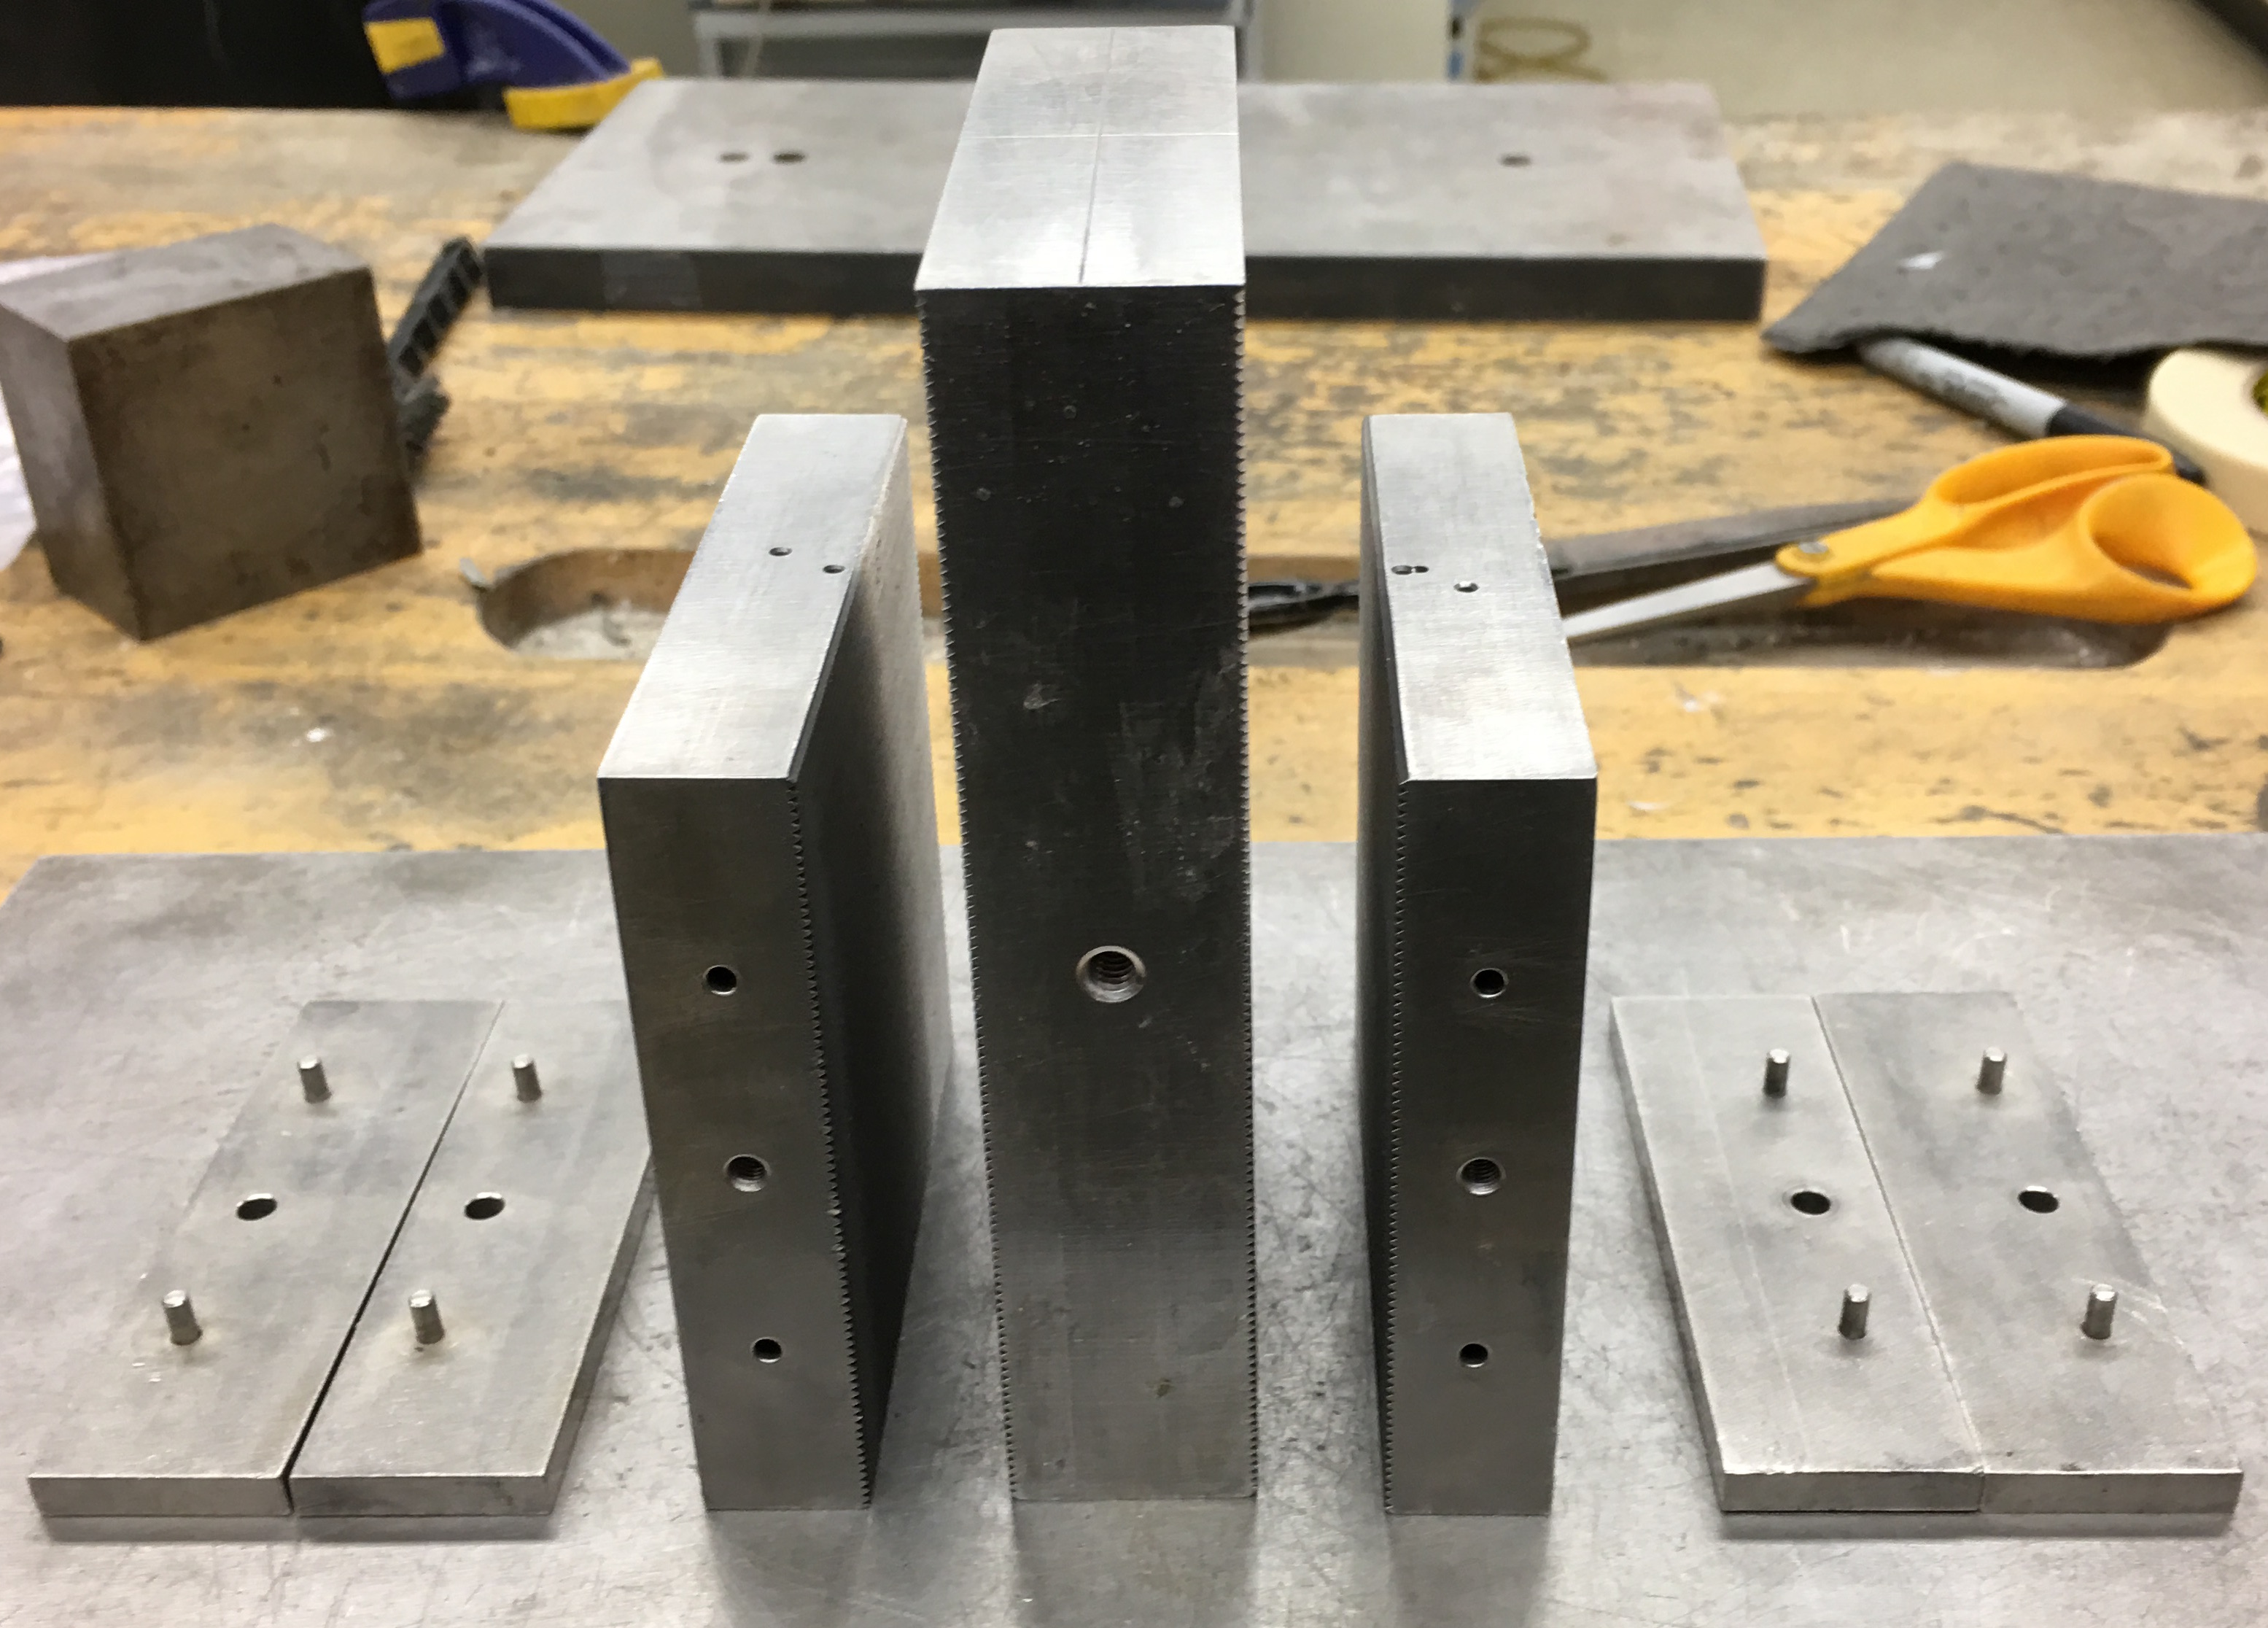
\includegraphics[width=0.7\textwidth]{appendix_sample_prep/dds_clean_blocks.jpg}
   	\caption{Gather all blocks and ensure that they are clean and free of debris.}
  	\label{Fig:dds_clean}
\end{figure}
%% End Figure %%

%% Figure %%
\begin{figure}
	\centering
        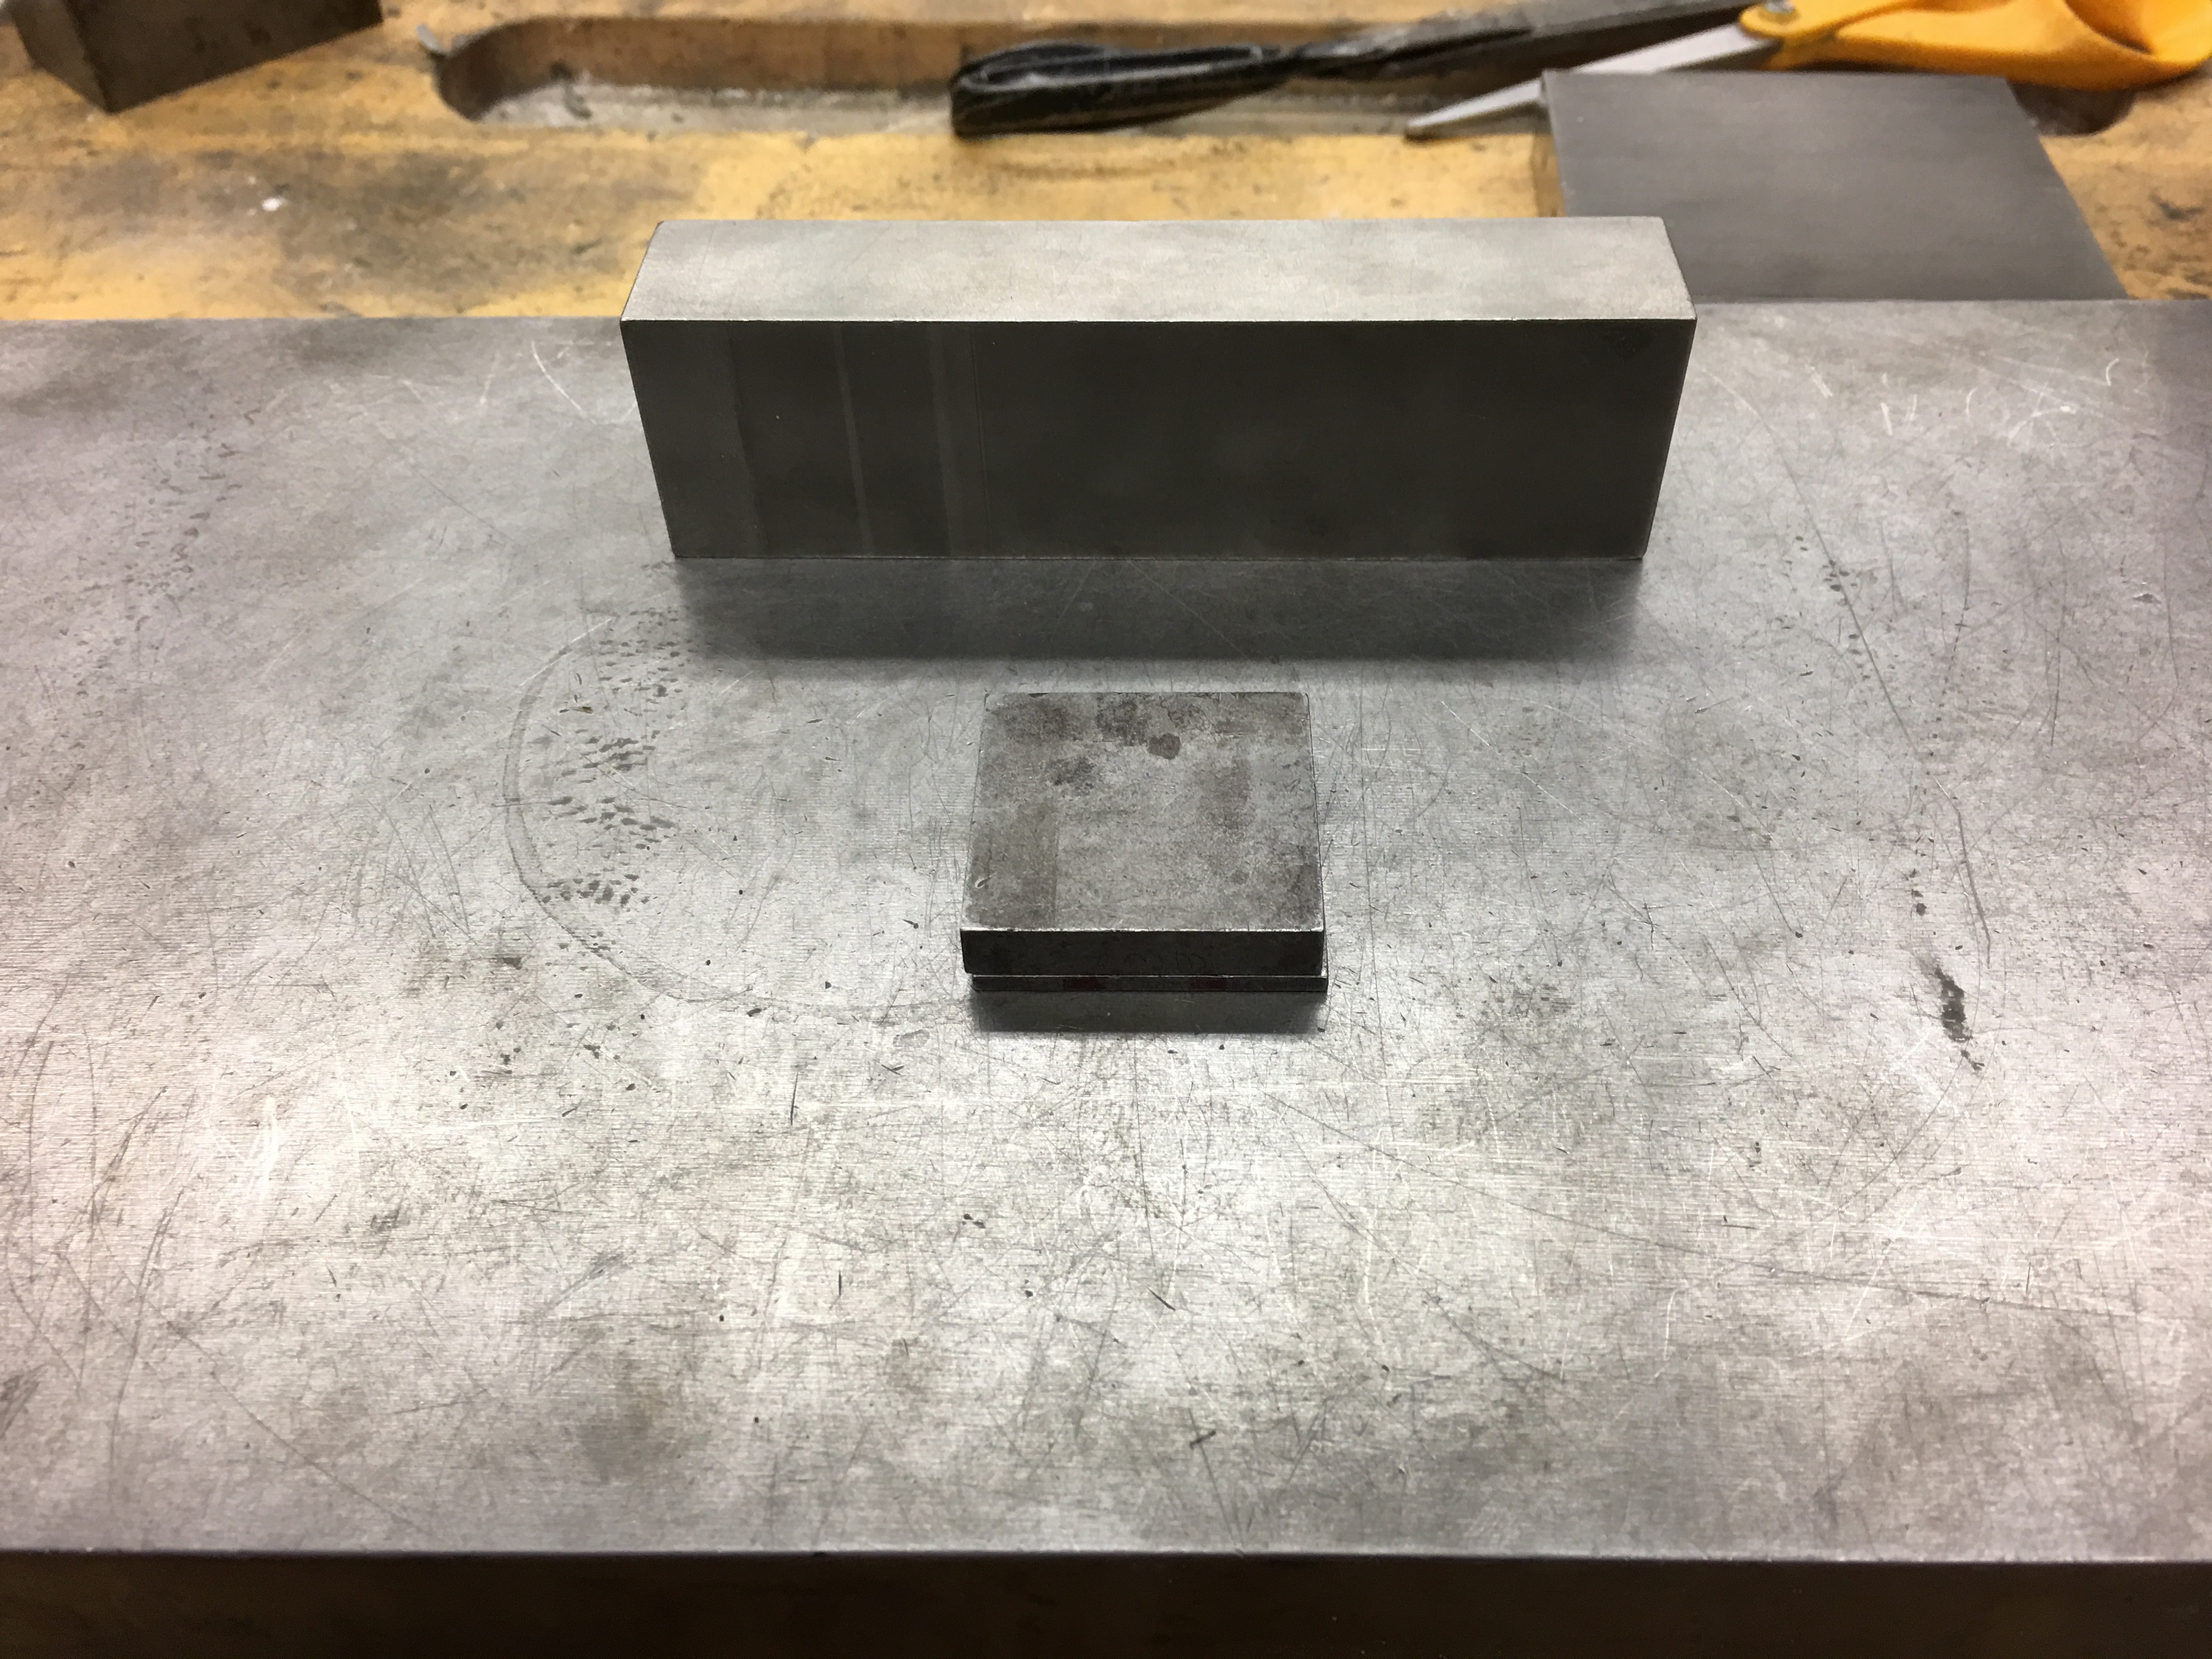
\includegraphics[width=0.7\textwidth]{appendix_sample_prep/dds_thickness_blocks.jpg}
   	\caption{Stack shims to adjust the sample thickness. Note which shims are used.}
  	\label{Fig:dds_thickness_blocks}
\end{figure}
%% End Figure %%

%% Figure %%
\begin{figure}
	\centering
        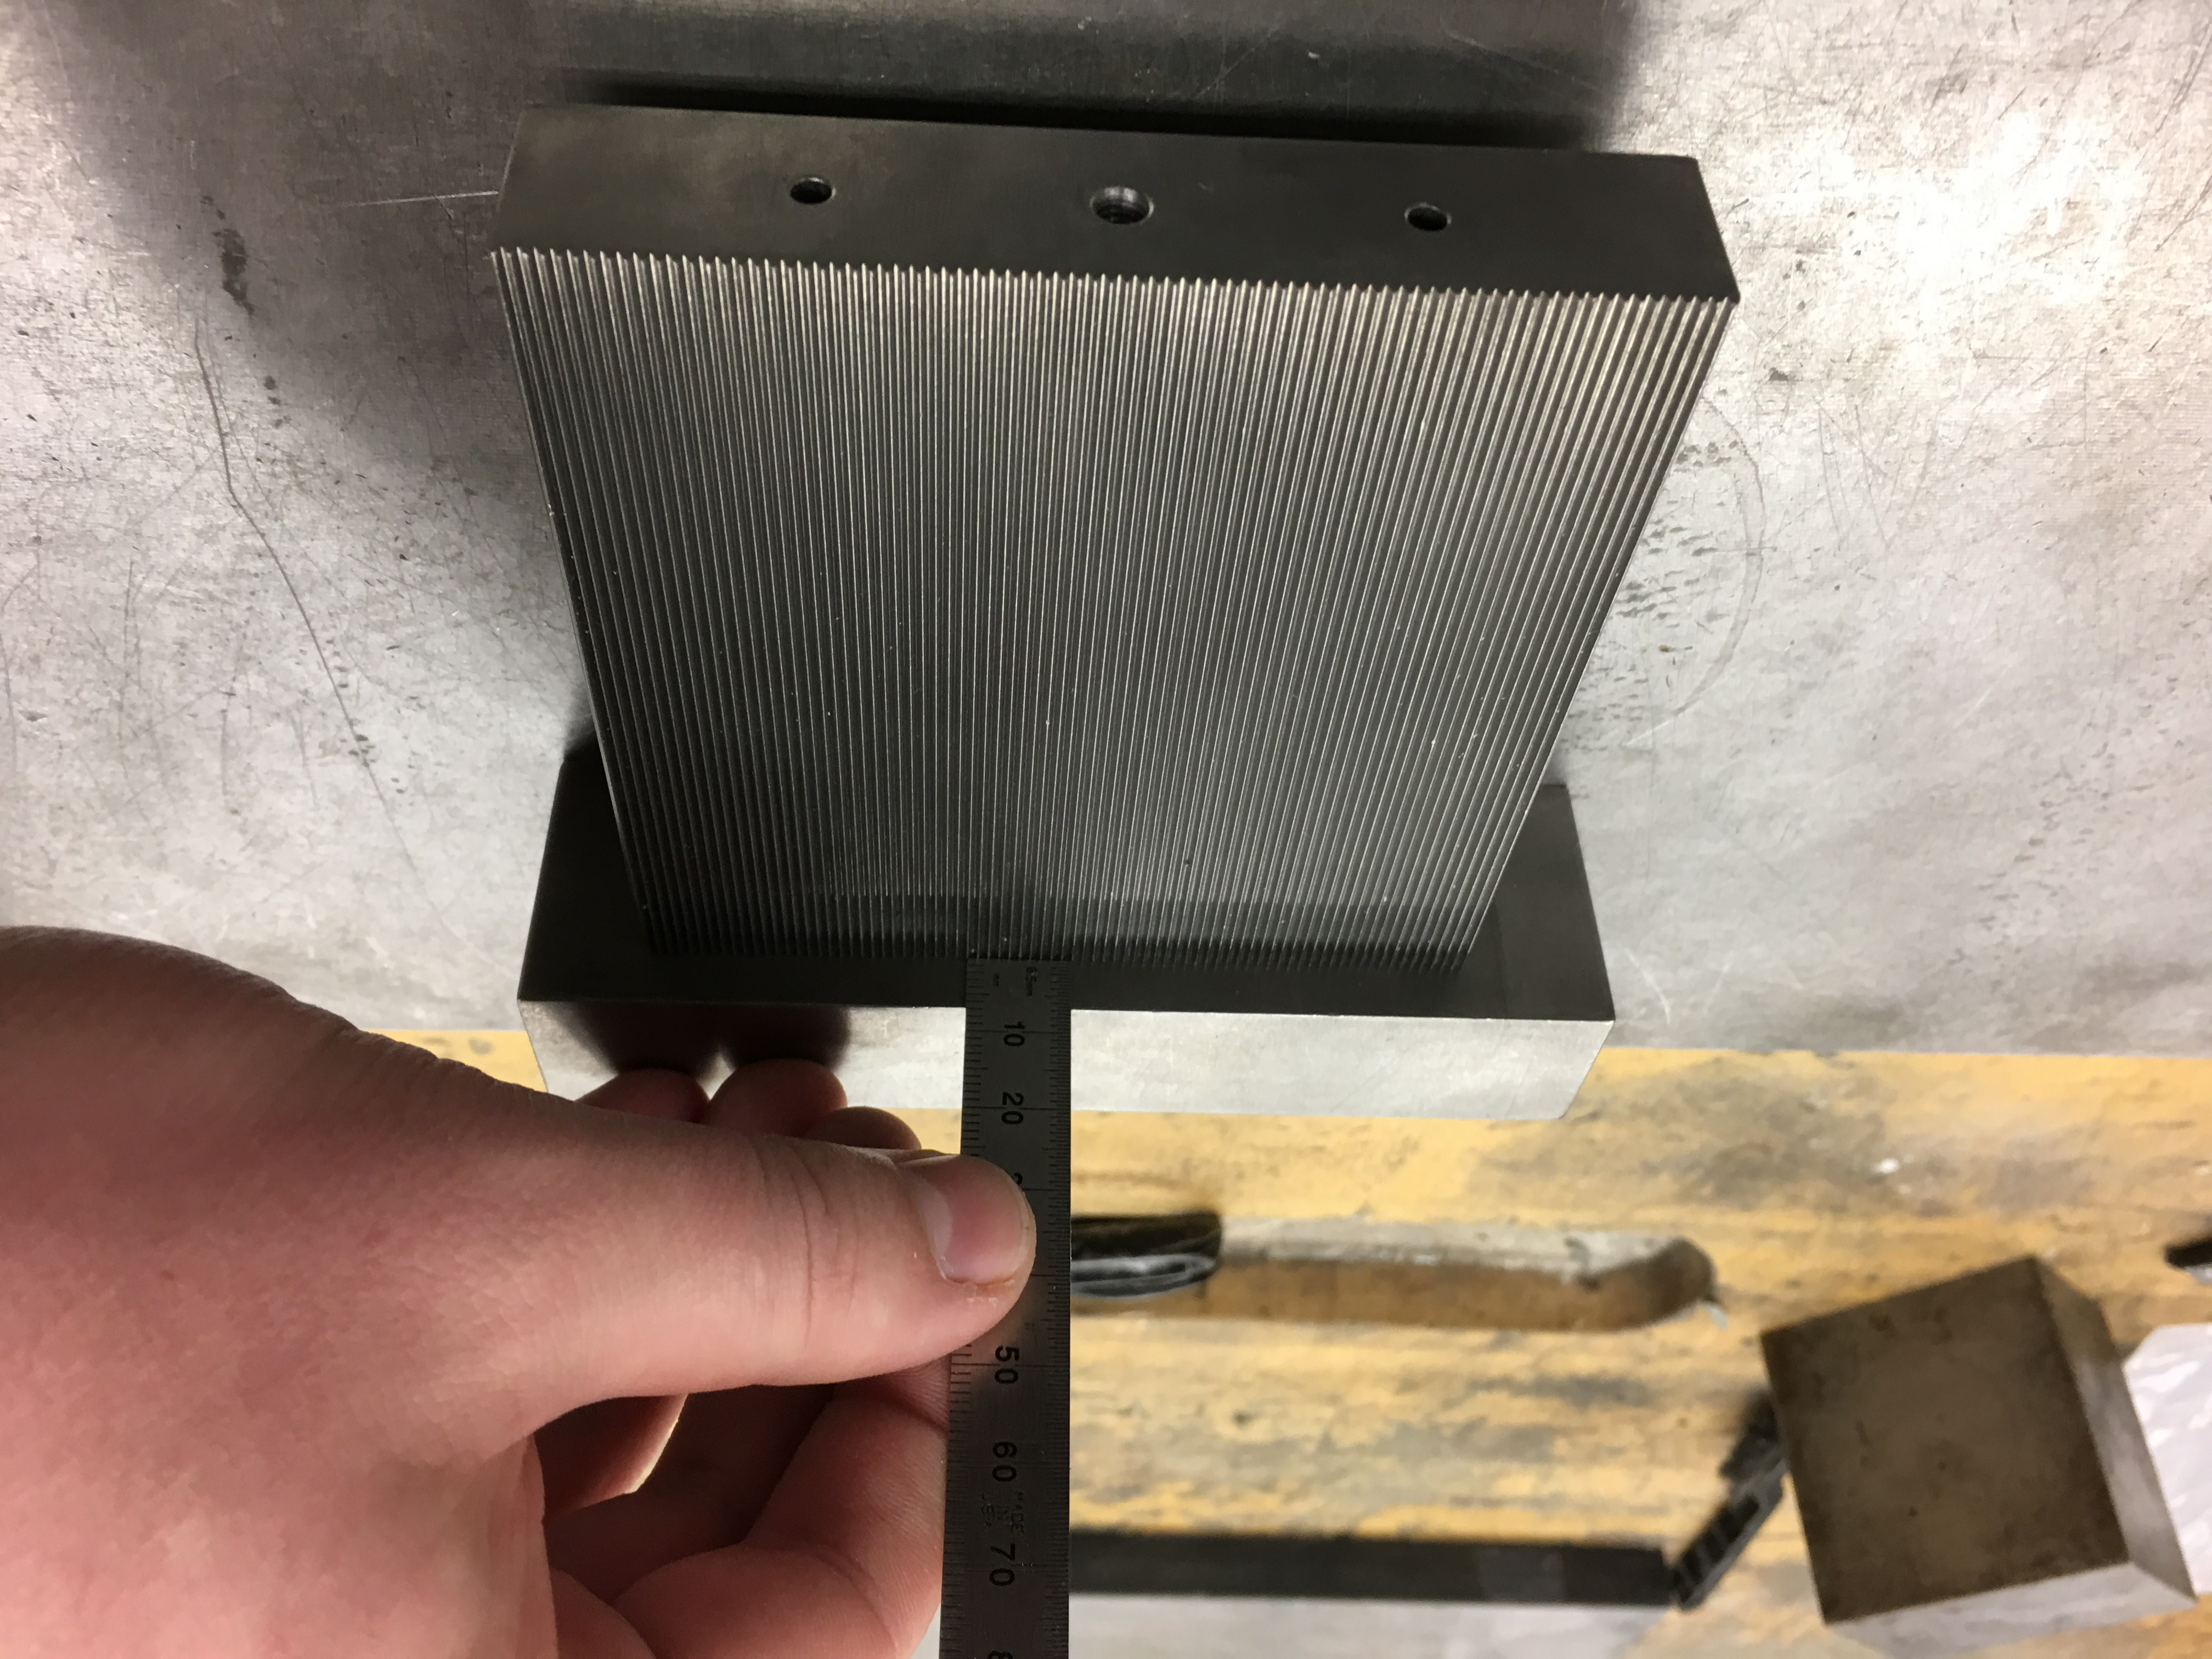
\includegraphics[width=0.7\textwidth]{appendix_sample_prep/dds_thickness_meas.jpg}
   	\caption{Measuring the sample thickness with a steel rule.}
  	\label{Fig:dds_thickness_meas}
\end{figure}
%% End Figure %%

%% Figure %%
\begin{figure}
	\centering
        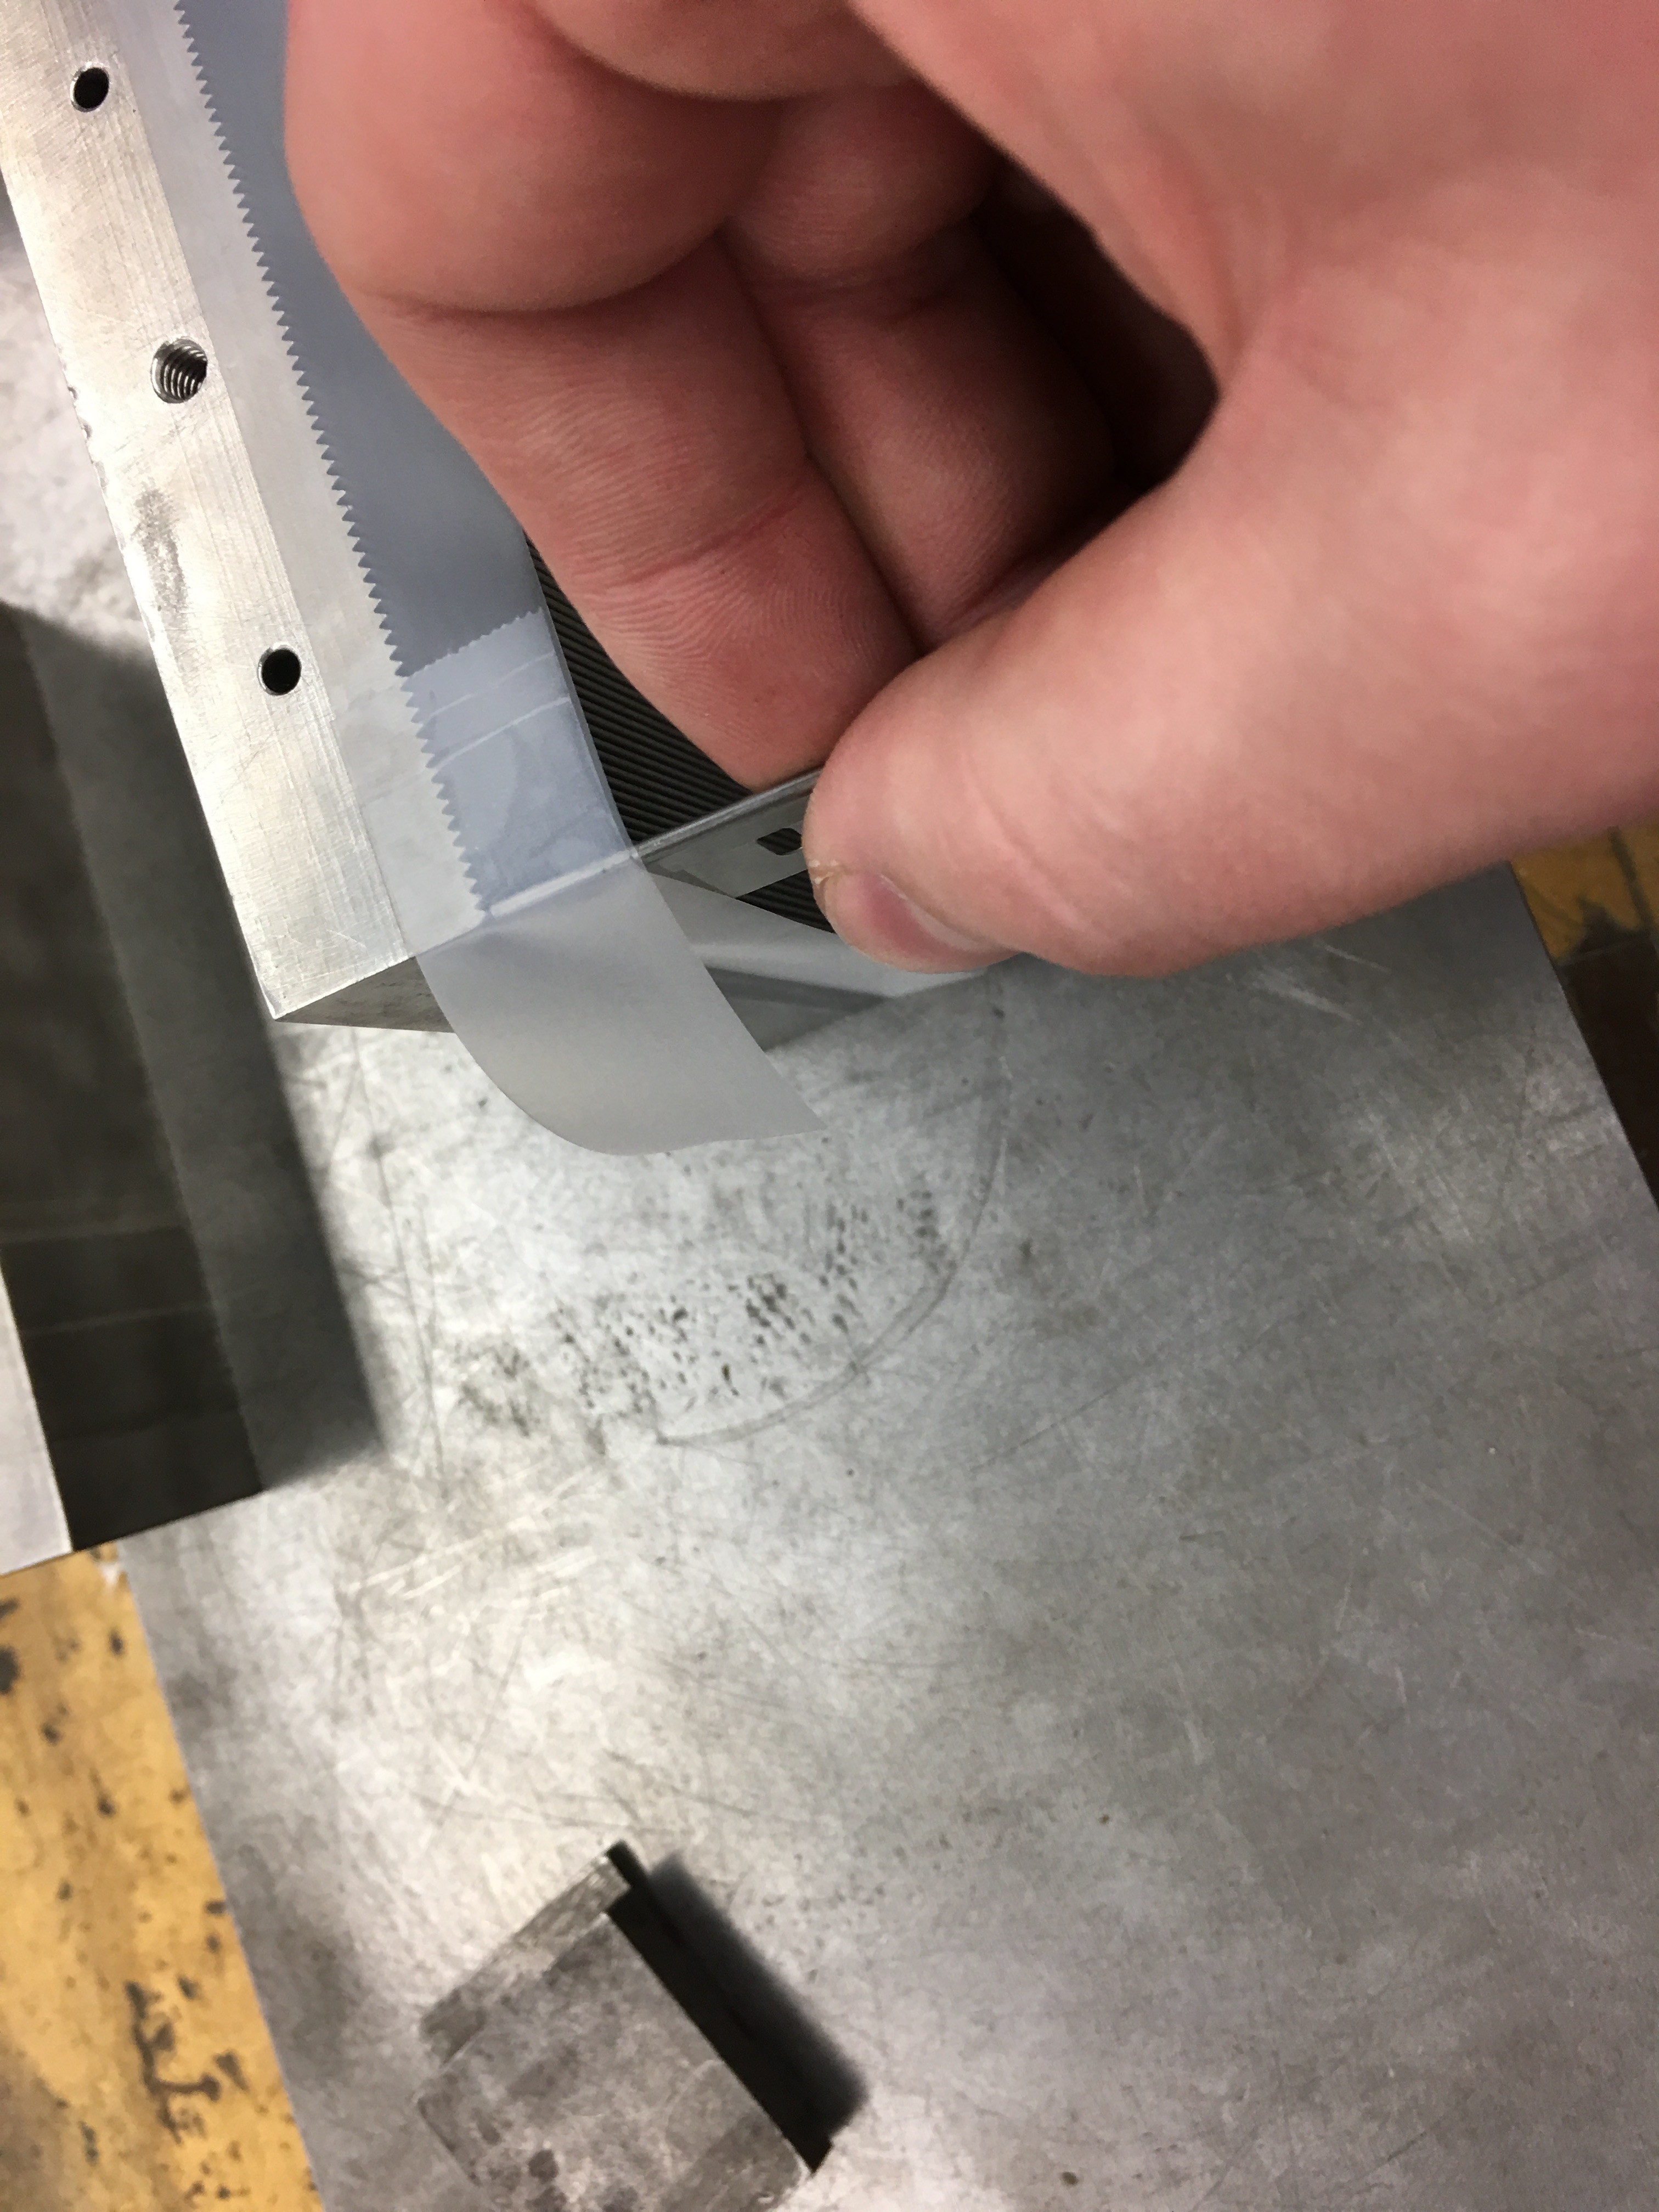
\includegraphics[width=0.7\textwidth]{appendix_sample_prep/dds_wrap_trim.jpg}
   	\caption{Carefully fold over the corner of the tape and trim any excess length.}
  	\label{Fig:dds_wrap_trim}
\end{figure}
%% End Figure %%

\clearpage

%% Figure %%
\begin{figure}
	\centering
        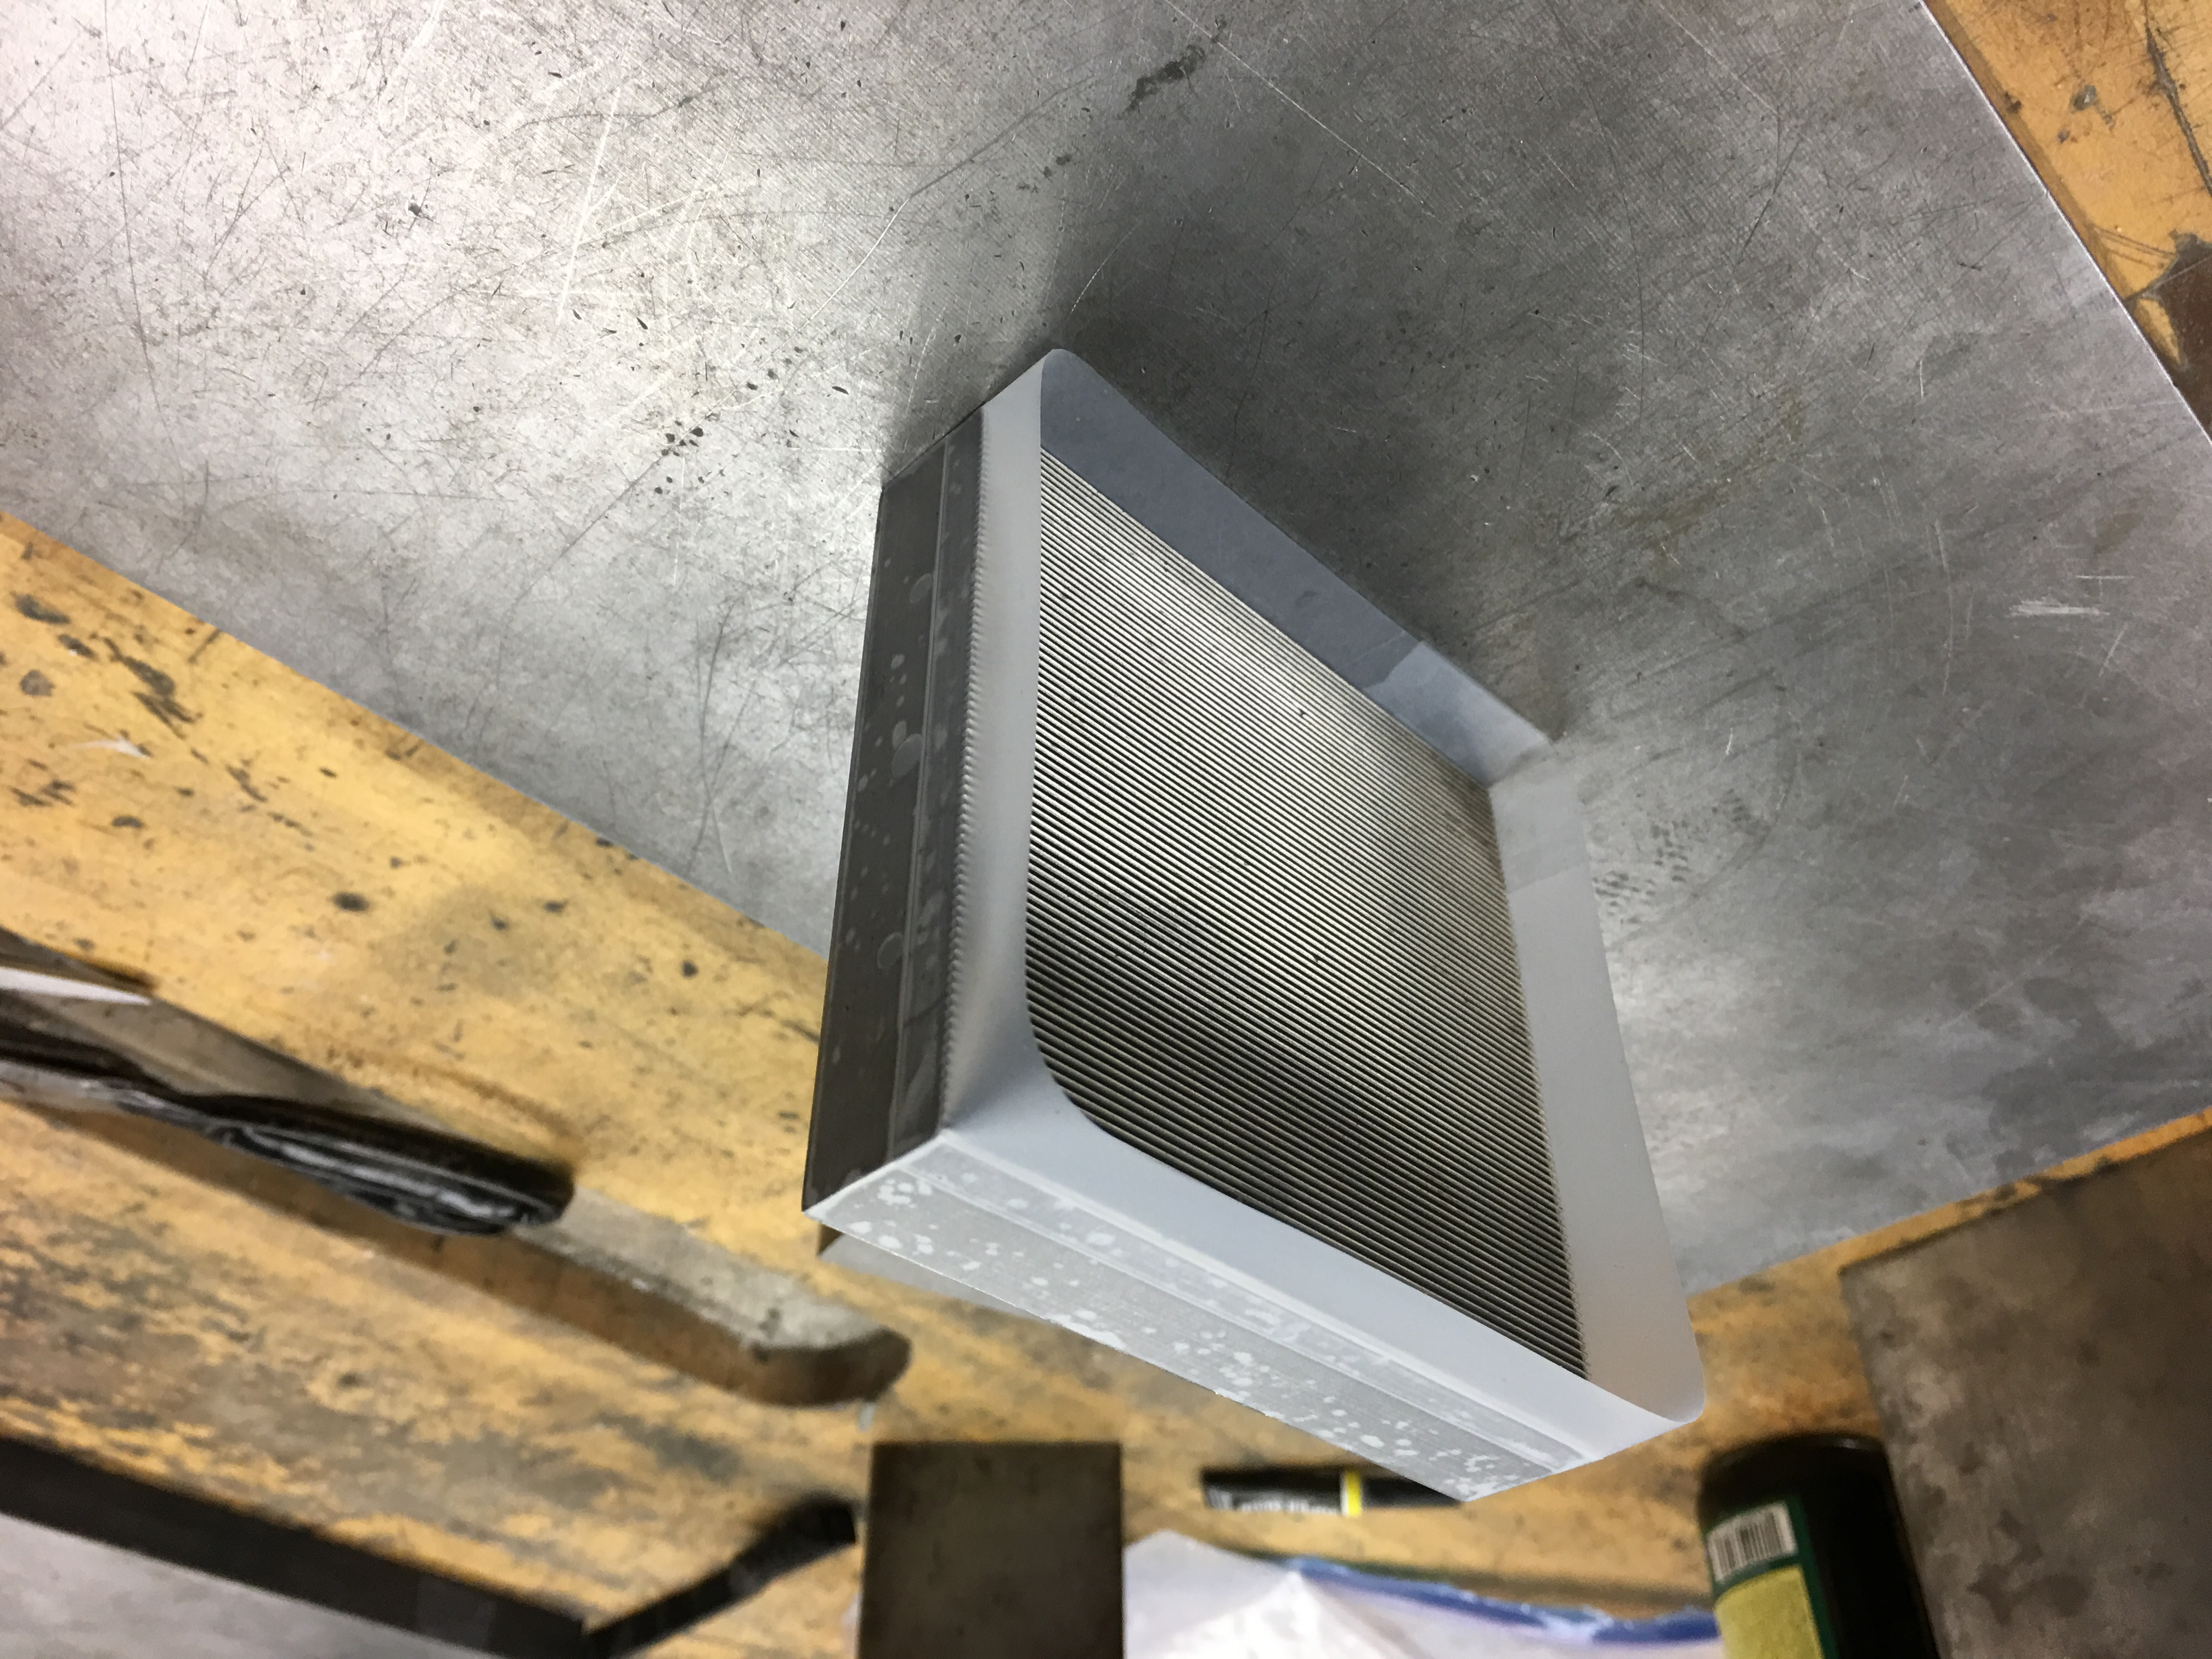
\includegraphics[width=0.7\textwidth]{appendix_sample_prep/dds_two_tape_layers.jpg}
   	\caption{A fully taped side block.}
  	\label{Fig:dds_two_tape_layers}
\end{figure}
%% End Figure %%

%% Figure %%
\begin{figure}
	\centering
        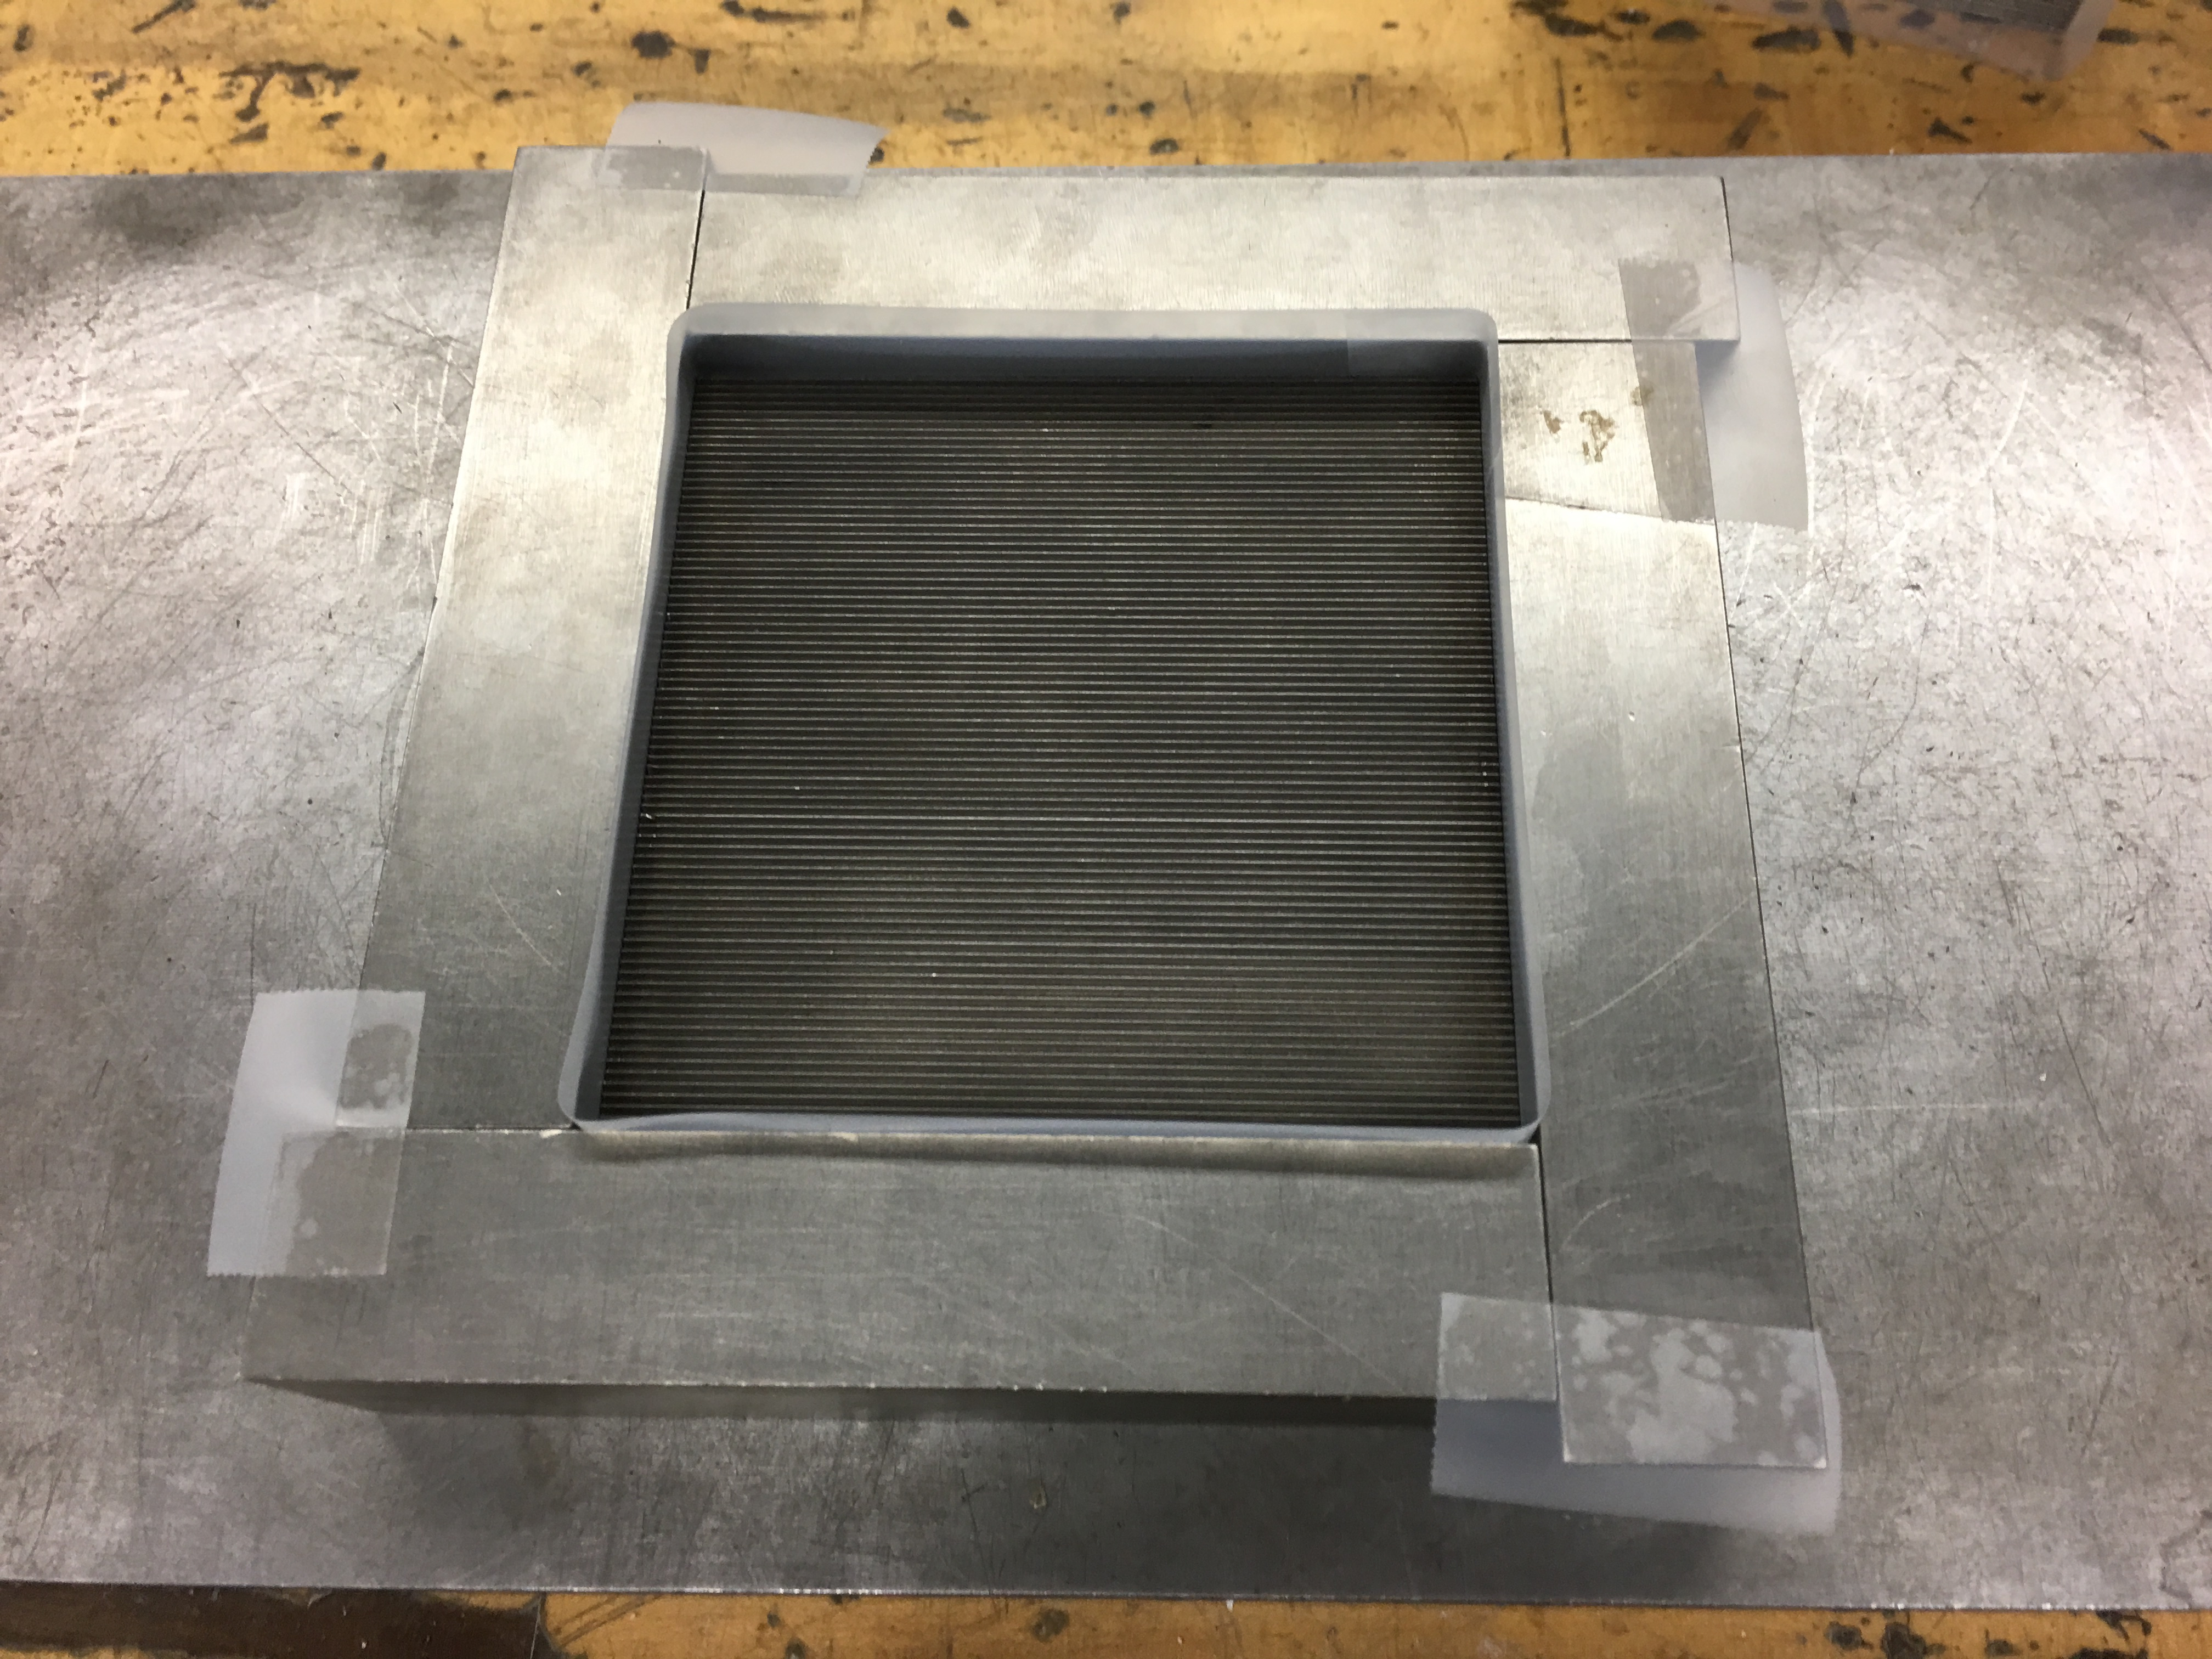
\includegraphics[width=0.7\textwidth]{appendix_sample_prep/dds_trim_setup.jpg}
   	\caption{Setup a jig to trim the excess tape height.}
  	\label{Fig:dds_trim_setup}
\end{figure}
%% End Figure %%

%% Figure %%
\begin{figure}
	\centering
        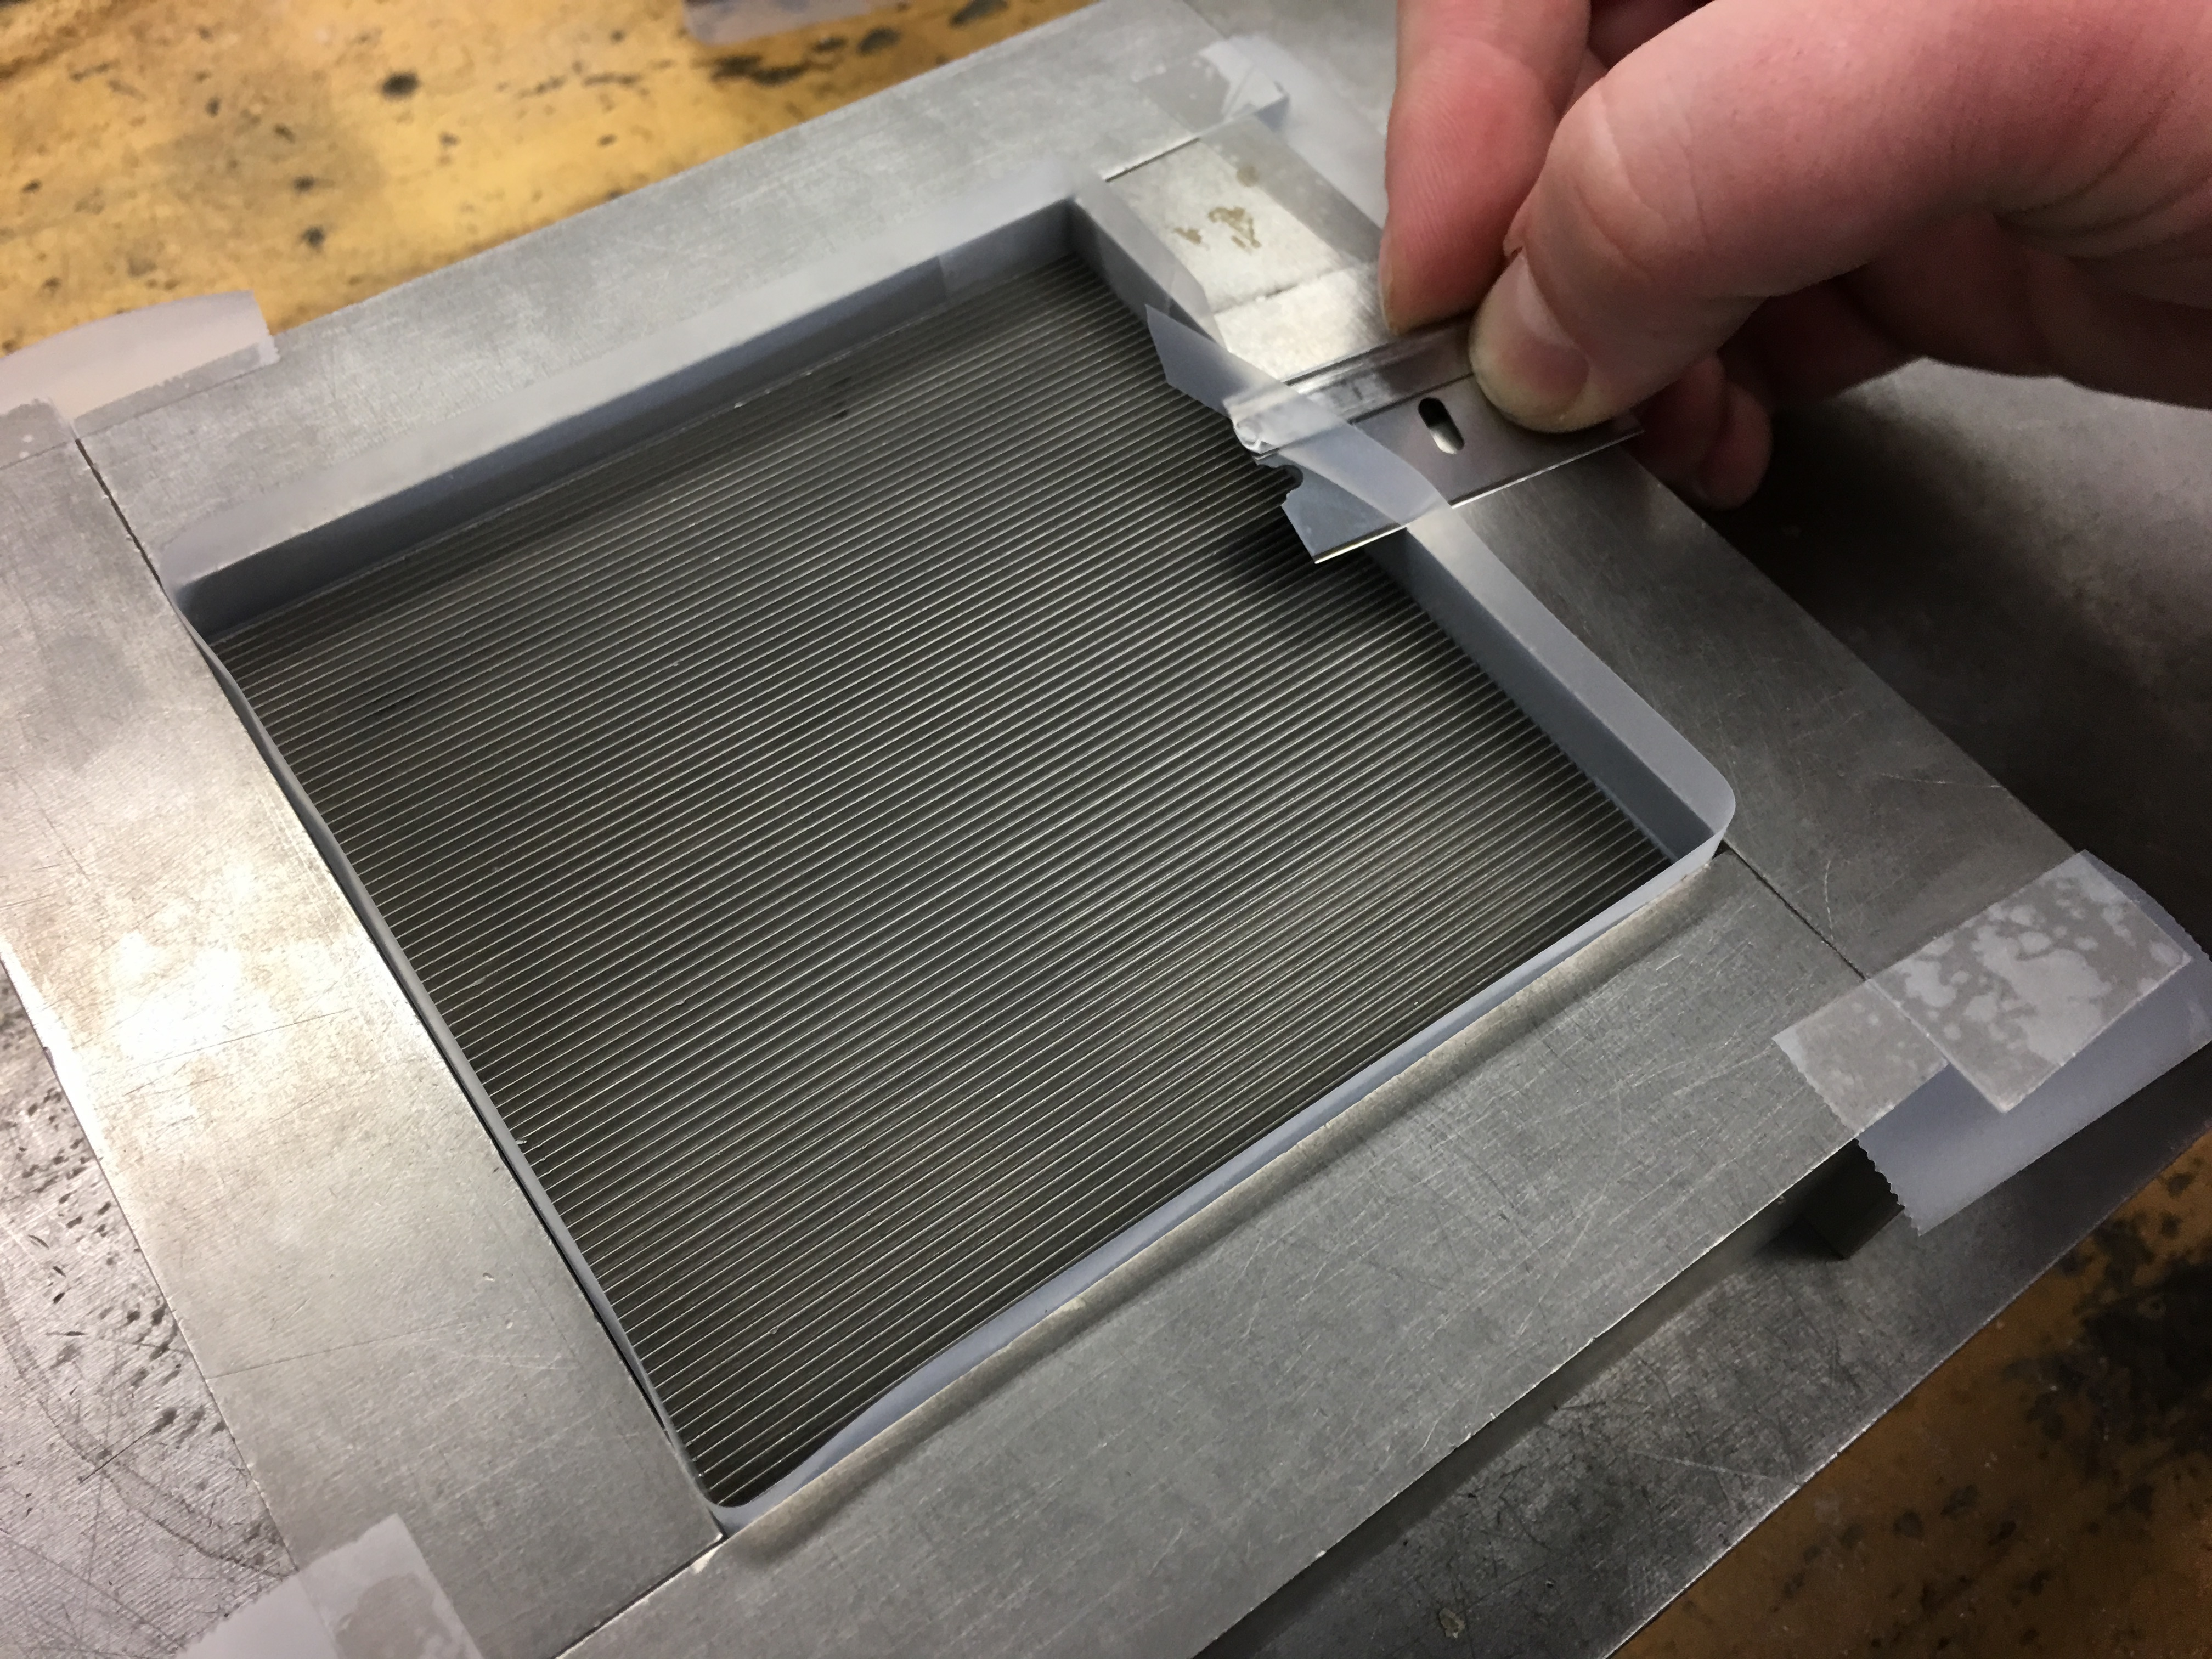
\includegraphics[width=0.7\textwidth]{appendix_sample_prep/dds_tape_trim.jpg}
   	\caption{Carefully trim the tape on all four sides of the block. Note the angle of the razor blade.}
  	\label{Fig:dds_tape_trim}
\end{figure}
%% End Figure %%

%% Figure %%
\begin{figure}
	\centering
        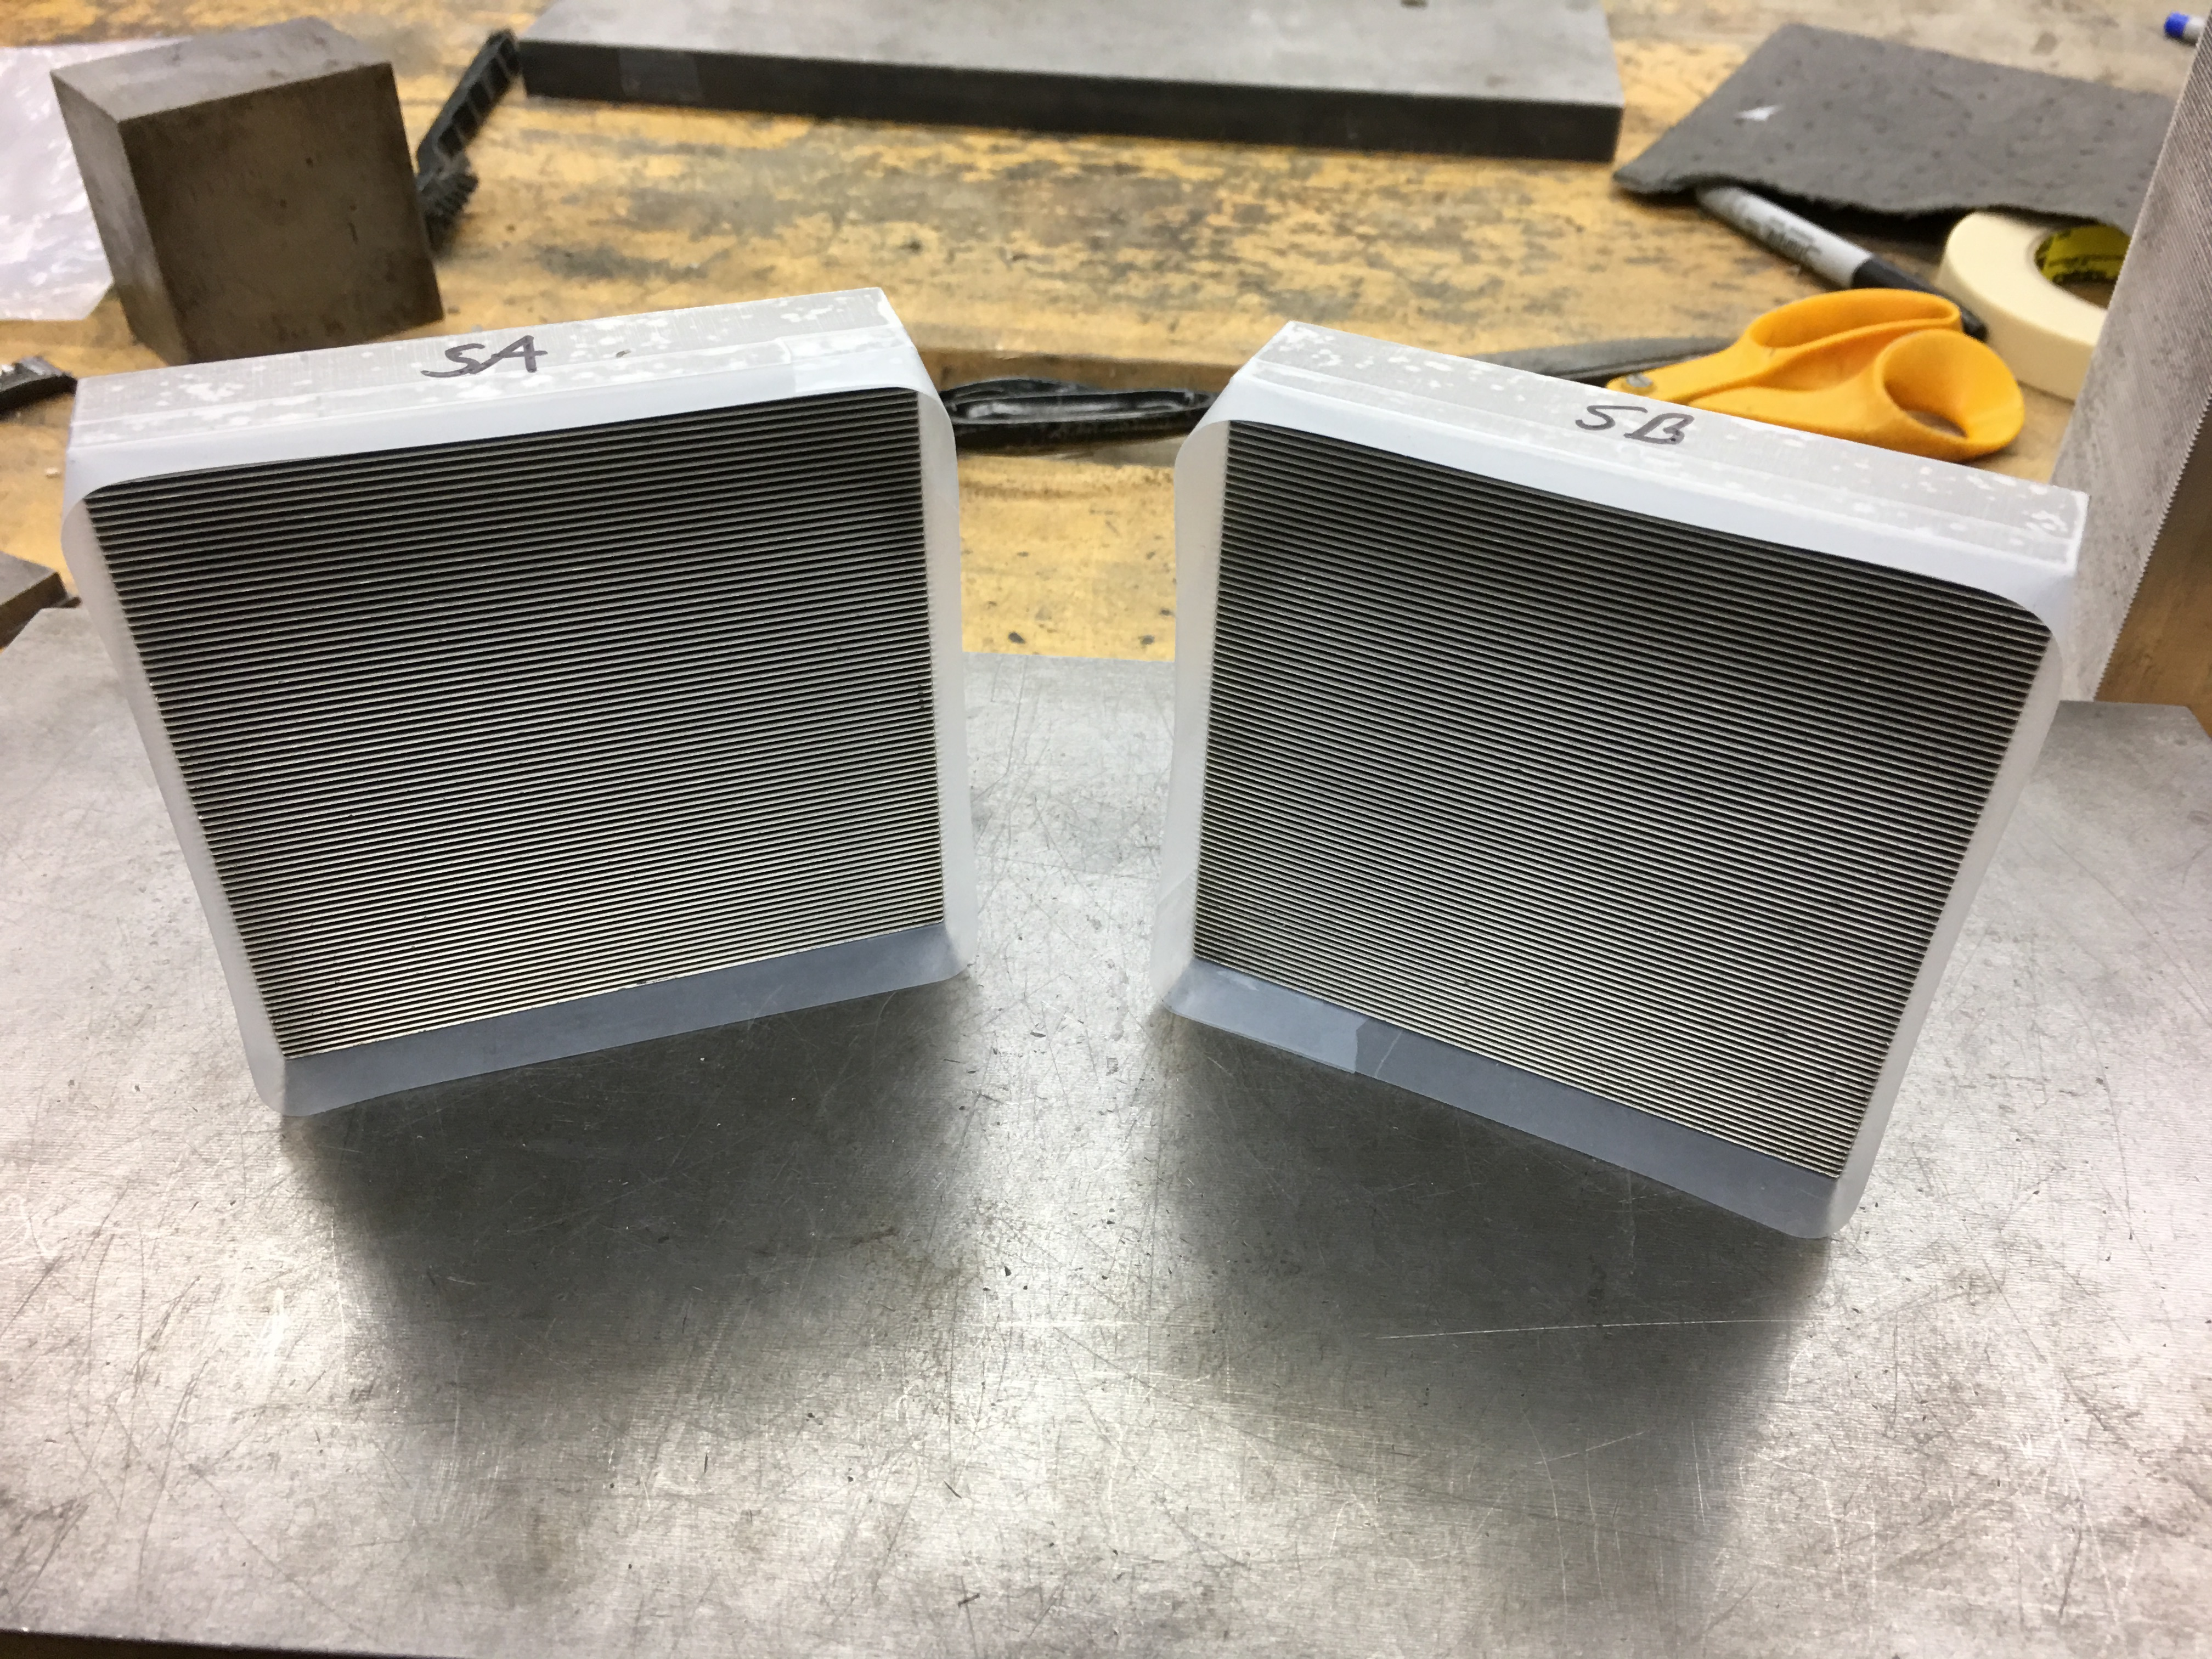
\includegraphics[width=0.7\textwidth]{appendix_sample_prep/dds_blocks_labeled.jpg}
   	\caption{Label the side blocks to help keep track of the mass of material in each layer.}
  	\label{Fig:dds_blocks_labeled}
\end{figure}
%% End Figure %%

\clearpage

%% Figure %%
\begin{figure}
	\centering
        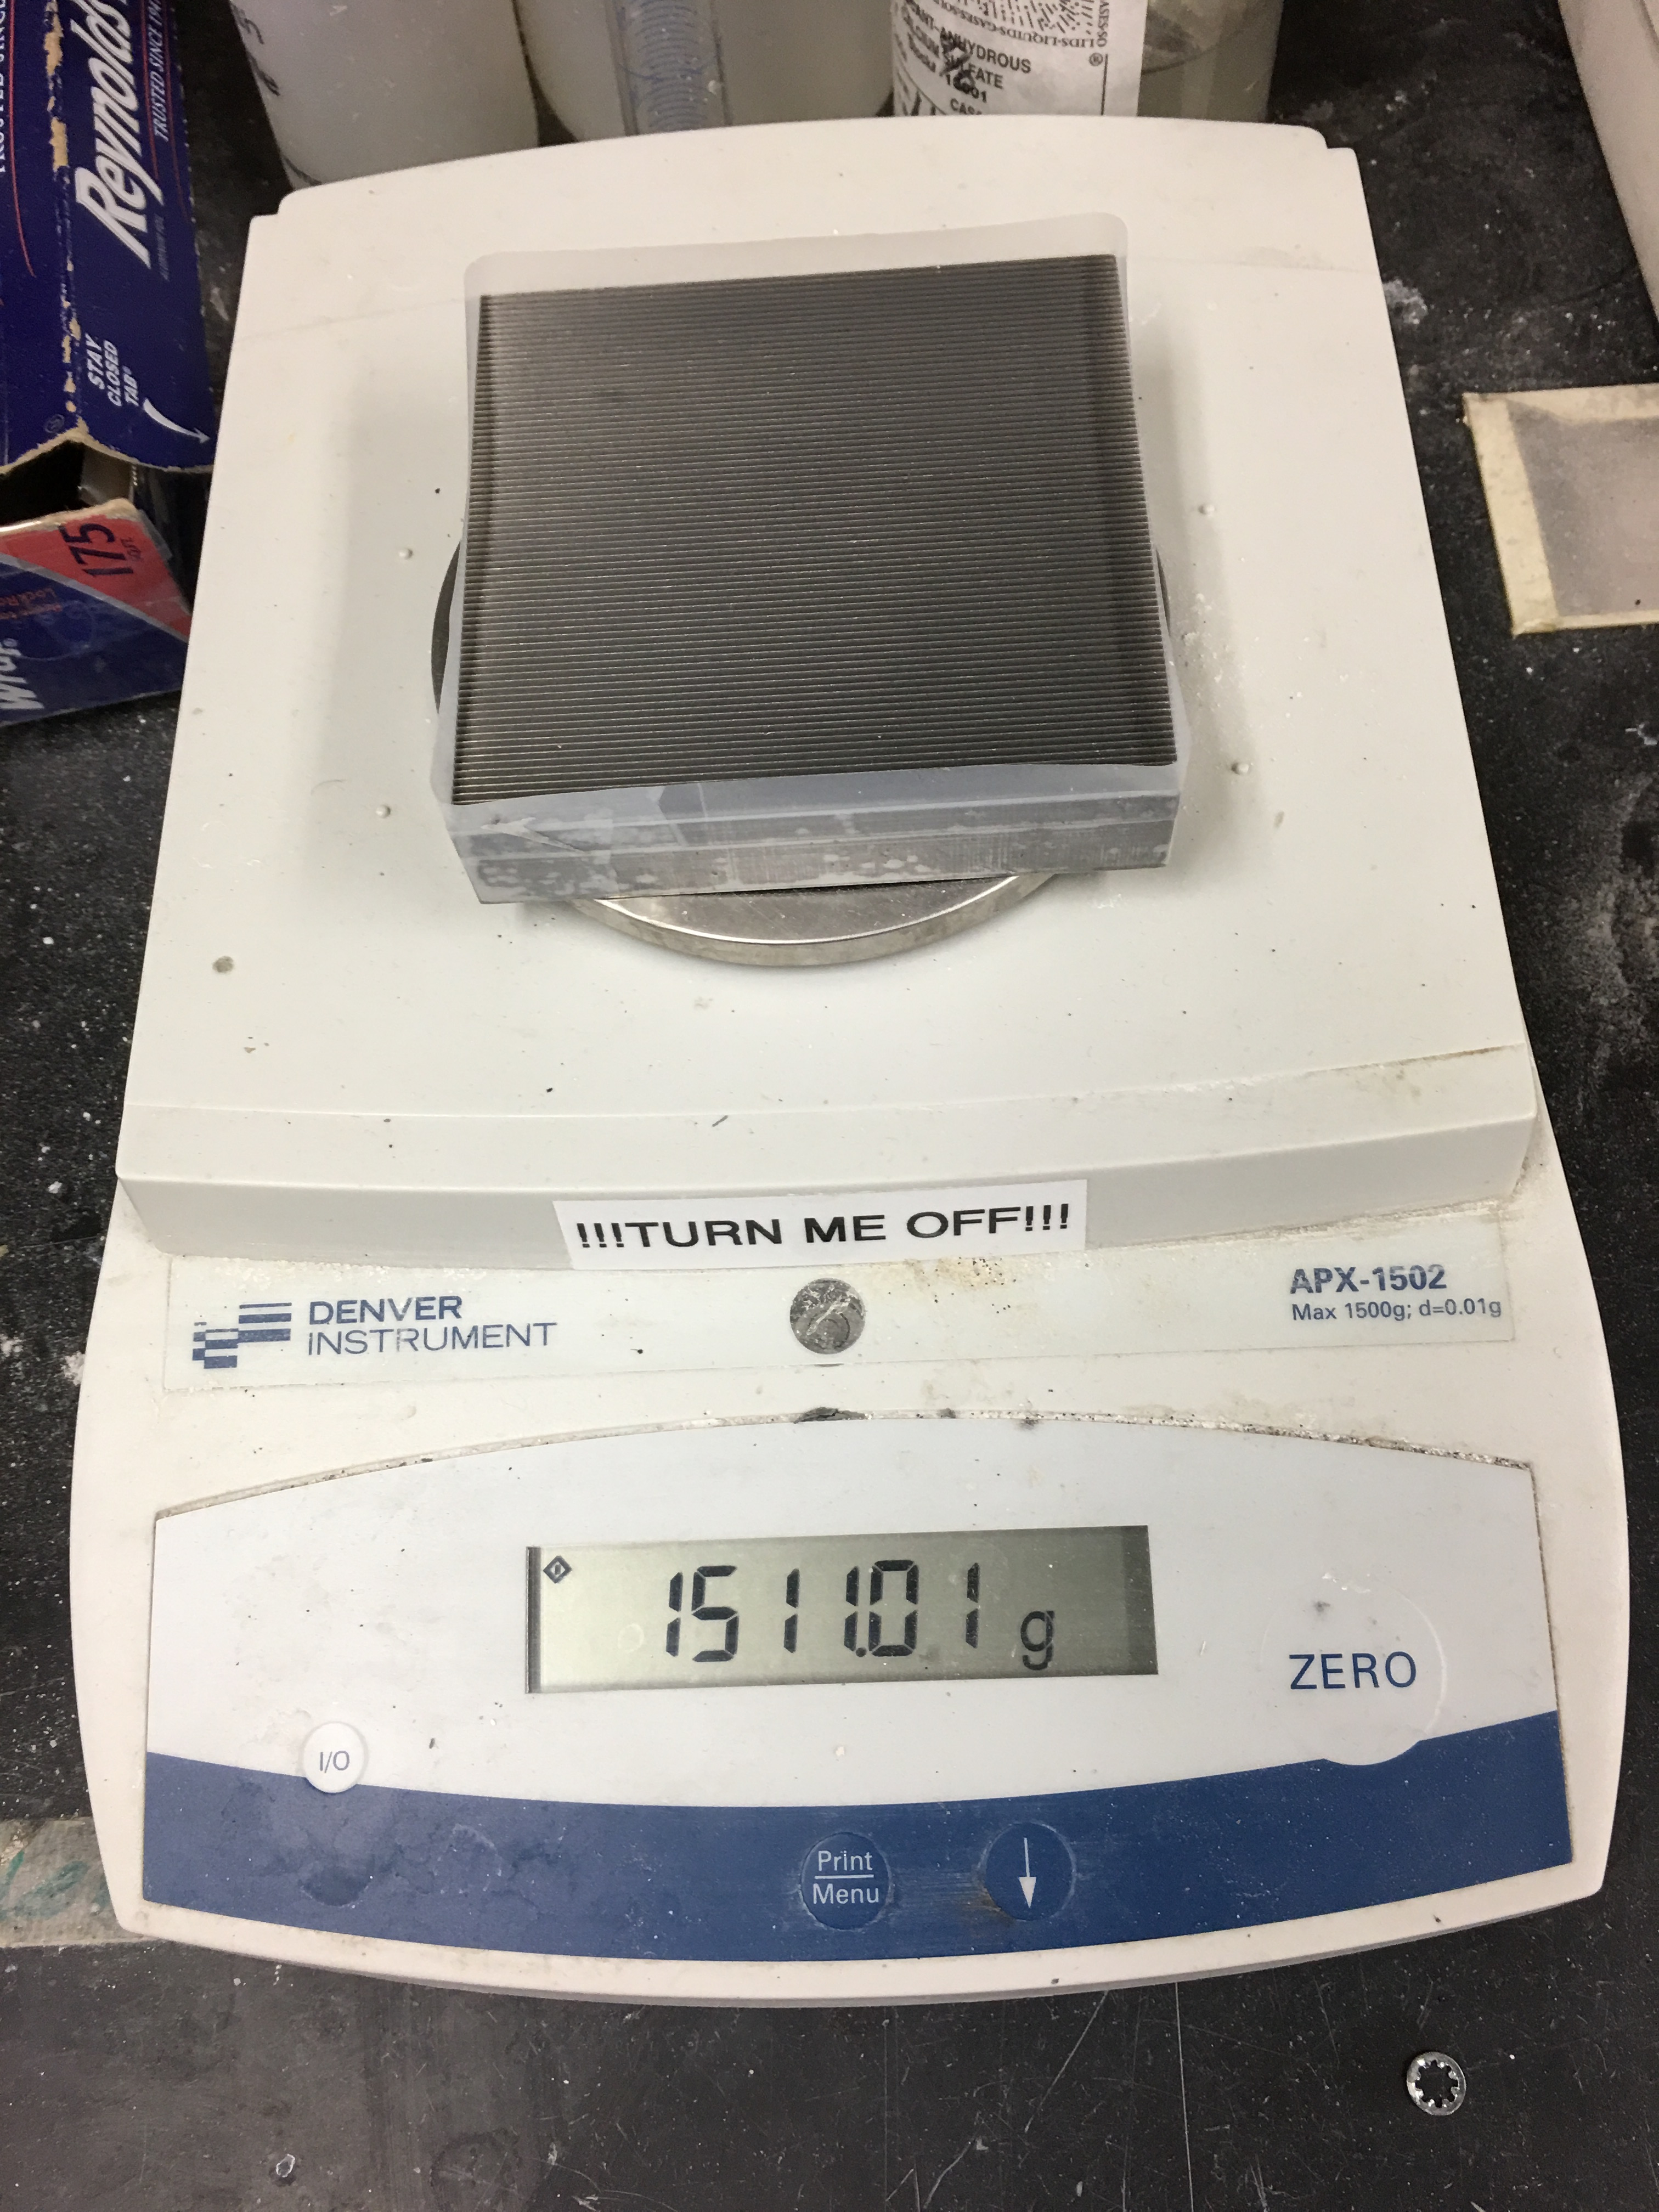
\includegraphics[width=0.7\textwidth]{appendix_sample_prep/dds_block_weight.jpg}
   	\caption{Weigh the blocks after all taping and trimming is completed.}
  	\label{Fig:dds_block_weight}
\end{figure}
%% End Figure %%

%% Figure %%
\begin{figure}
	\centering
        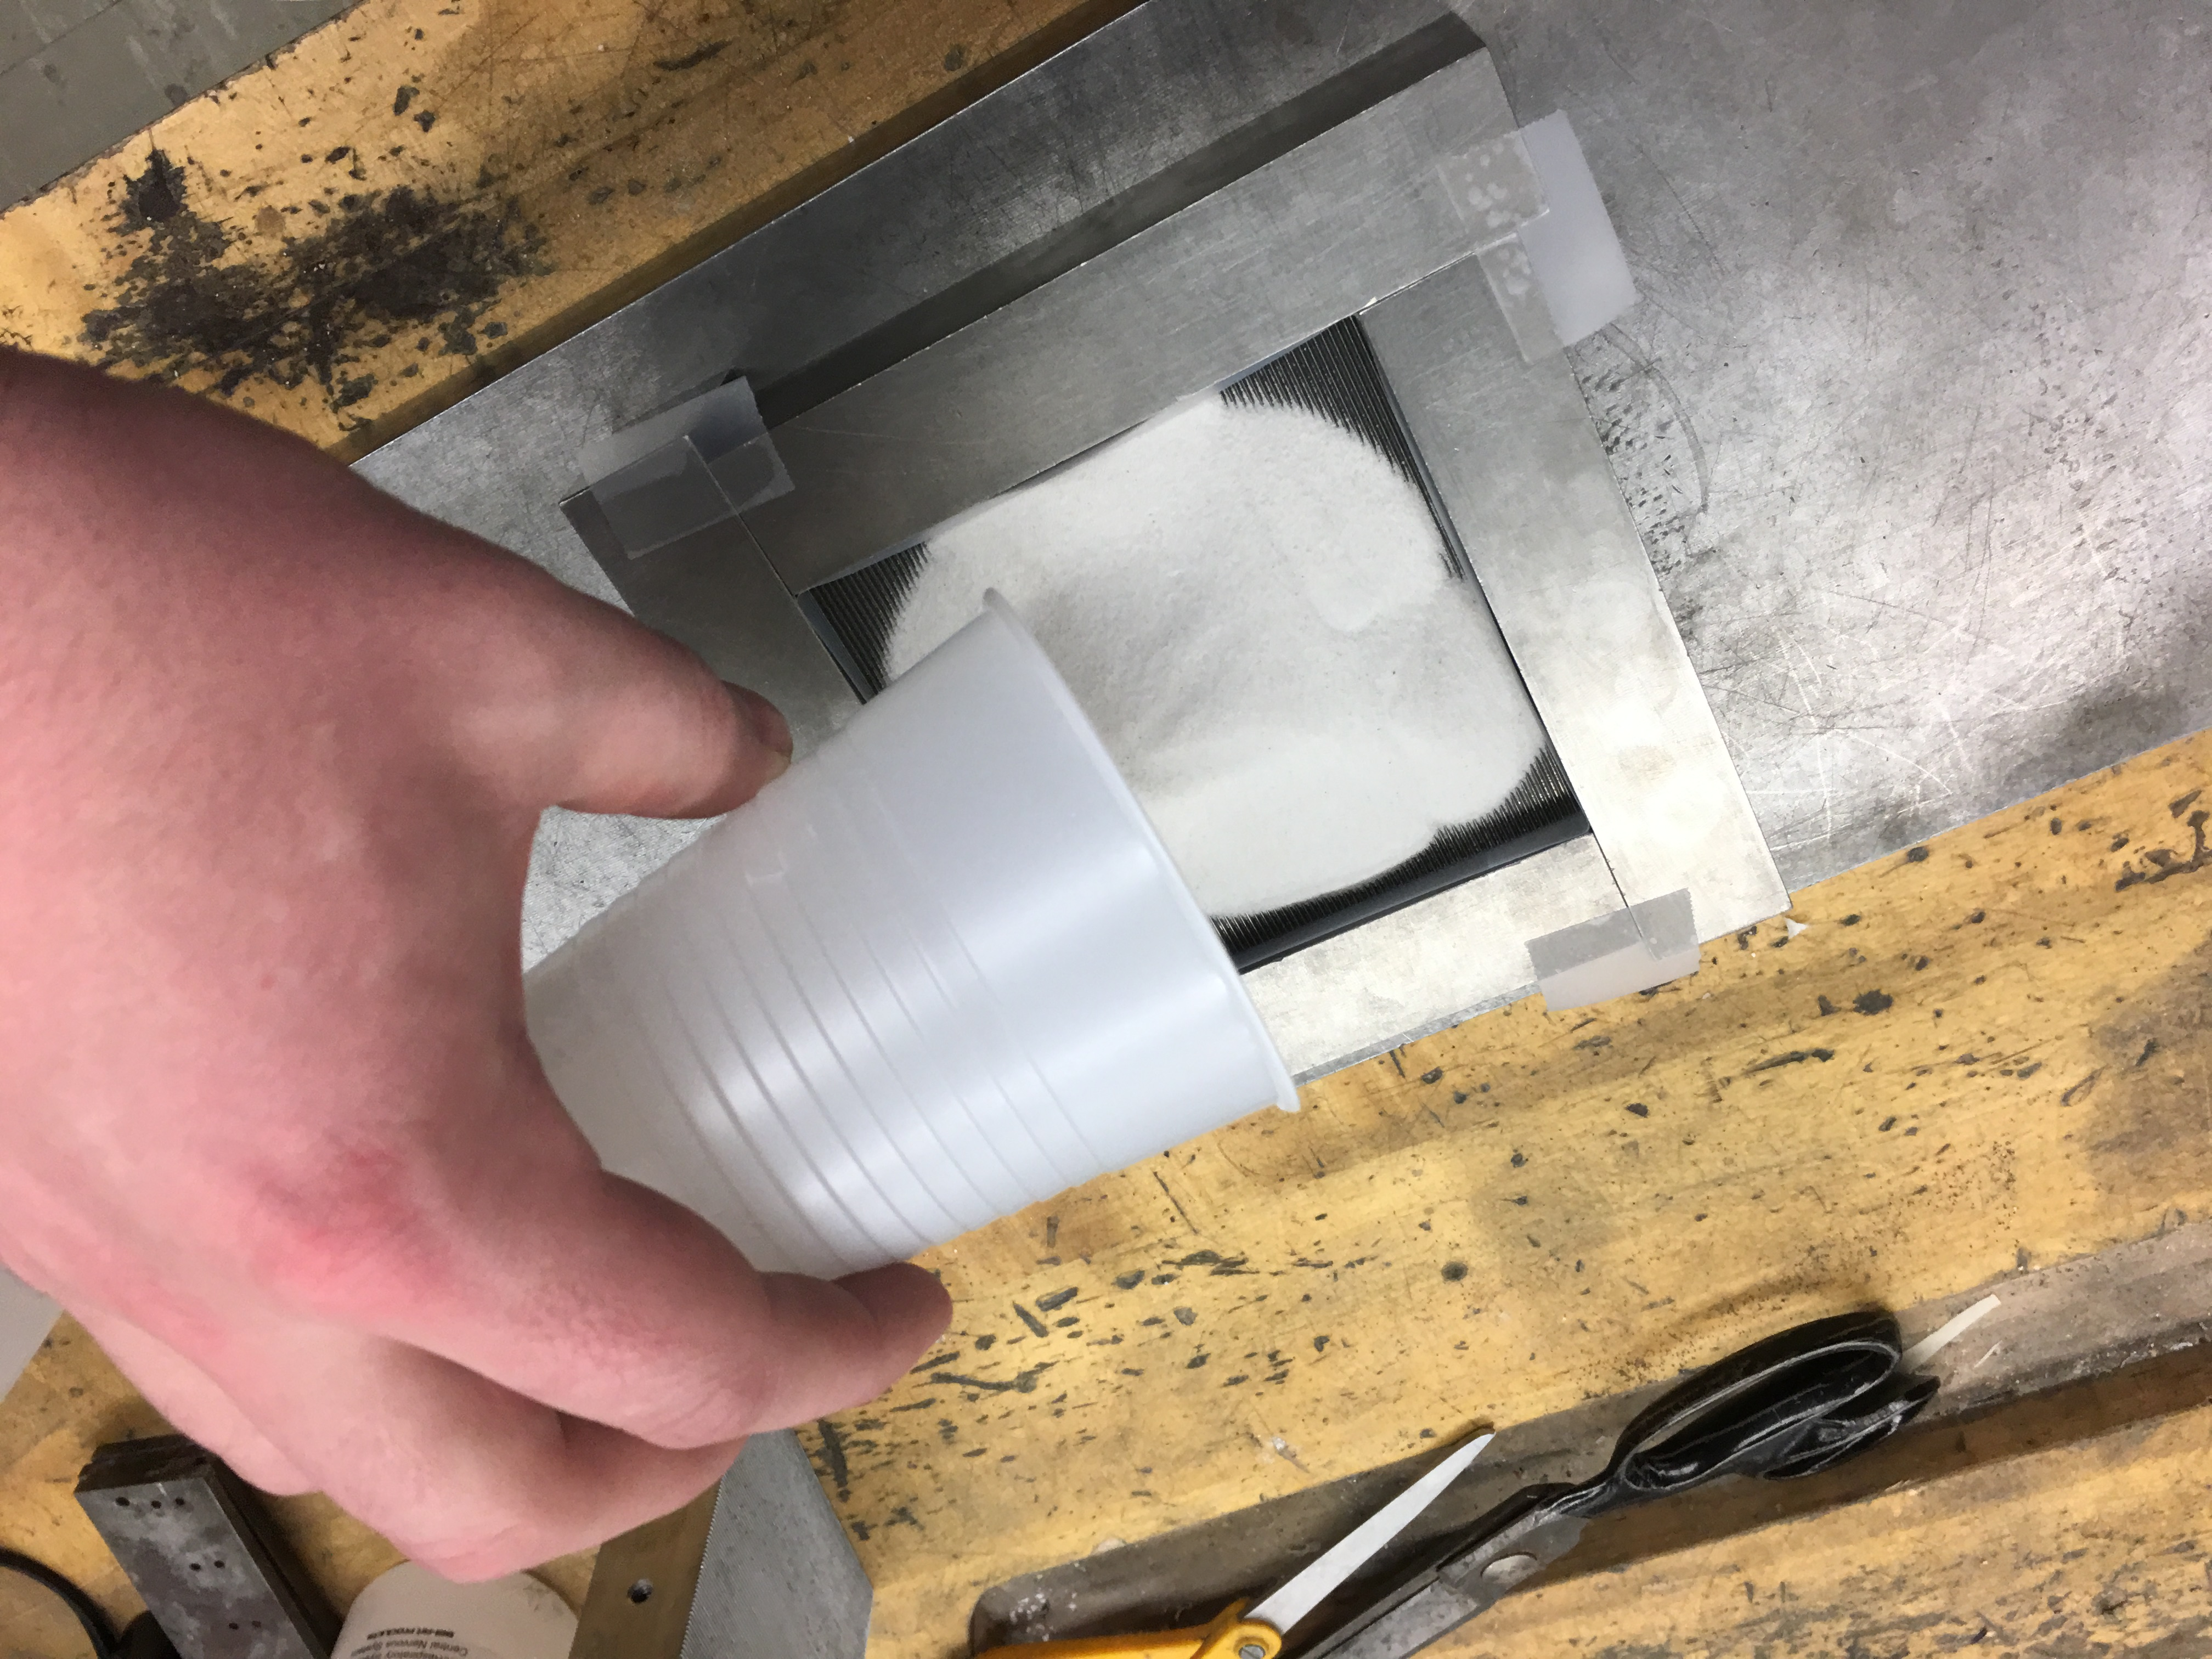
\includegraphics[width=0.7\textwidth]{appendix_sample_prep/dds_pour_material.jpg}
   	\caption{Carefully pour sample material into the taped area of the block.}
  	\label{Fig:dds_pour_material}
\end{figure}
%% End Figure %%

%% Figure %%
\begin{figure}
	\centering
        \includegraphics[width=0.7\textwidth]{appendix_sample_prep/dds_cutup_sample.jpg}
   	\caption{Using a sliding and chopping action, evenly distribute the sample material over the side block.}
  	\label{Fig:dds_cutup_sample}
\end{figure}
%% End Figure %%

%% Figure %%
\begin{figure}
	\centering
        \includegraphics[width=0.7\textwidth]{appendix_sample_prep/dds_press_sample.jpg}
   	\caption{Firmly compress the sample to ensure a good granular packing.}
  	\label{Fig:dds_press_sample}
\end{figure}
%% End Figure %%

\clearpage

%% Figure %%
\begin{figure}
	\centering
        \includegraphics[width=0.7\textwidth]{appendix_sample_prep/dds_level_sample.jpg}
   	\caption{Drag the steel rule over the sample to flatten the layer.}
  	\label{Fig:dds_level_sample}
\end{figure}
%% End Figure %%

%% Figure %%
\begin{figure}
	\centering
        \includegraphics[width=0.7\textwidth]{appendix_sample_prep/dds_finished_sideblock.jpg}
   	\caption{A completed side block ready to be weighed and assembled.}
  	\label{Fig:dds_finished_sideblock}
\end{figure}
%% End Figure %%

%% Figure %%
\begin{figure}
	\centering
        \includegraphics[width=0.7\textwidth]{appendix_sample_prep/dds_ell_jig.jpg}
   	\caption{Setup the jig for assembling the side and center blocks into the complete sample assembly.}
  	\label{Fig:dds_ell_jig}
\end{figure}
%% End Figure %%

%% Figure %%
\begin{figure}
	\centering
        \includegraphics[width=0.7\textwidth]{appendix_sample_prep/dds_sideblock_jig.jpg}
   	\caption{Place the sideblock into the jig with the side shield mounts facing towards you.}
  	\label{Fig:dds_sideblock_jig}
\end{figure}
%% End Figure %%

\clearpage

%% Figure %%
\begin{figure}
	\centering
        \includegraphics[width=0.7\textwidth]{appendix_sample_prep/dds_sideblock_jig_2.jpg}
   	\caption{Place a spacer at the top of the side block to help support the center block's weight.}
  	\label{Fig:dds_sideblock_jig_2}
\end{figure}
%% End Figure %%

%% Figure %%
\begin{figure}
	\centering
        \includegraphics[width=0.7\textwidth]{appendix_sample_prep/dds_centerblock_jig.jpg}
   	\caption{Place the center block on and secure it with small strips of tape. Note the counterweight block on top of the center block.}
  	\label{Fig:dds_centerblock_jig}
\end{figure}
%% End Figure %%

%% Figure %%
\begin{figure}
	\centering
        \includegraphics[width=0.7\textwidth]{appendix_sample_prep/dds_move_block.jpg}
   	\caption{Rearrange the jig so that the sample can be taped without moving.}
  	\label{Fig:dds_move_block}
\end{figure}
%% End Figure %%

%% Figure %%
\begin{figure}
	\centering
        \includegraphics[width=0.7\textwidth]{appendix_sample_prep/dds_one_strip_tape.jpg}
   	\caption{Place one strip of tape around the bottom and sides of the sample.}
  	\label{Fig:dds_one_strip_tape}
\end{figure}
%% End Figure %%

\clearpage

%% Figure %%
\begin{figure}
	\centering
        \includegraphics[width=0.7\textwidth]{appendix_sample_prep/dds_three_strip_tape.jpg}
   	\caption{Add two more strips of tape, each offset from the others to provide the best seal of the sample material.}
  	\label{Fig:dds_three_strip_tape}
\end{figure}
%% End Figure %%

%% Figure %%
\begin{figure}
	\centering
        \includegraphics[width=0.7\textwidth]{appendix_sample_prep/dds_standup_one_block.jpg}
   	\caption{Stand the assembly up on the workbench.}
  	\label{Fig:dds_standup_one_block}
\end{figure}
%% End Figure %%

%% Figure %%
\begin{figure}
	\centering
        \includegraphics[width=0.7\textwidth]{appendix_sample_prep/dds_one_block_taped.jpg}
   	\caption{Tape the top of the assembly.}
  	\label{Fig:dds_one_block_taped}
\end{figure}
%% End Figure %%

%% Figure %%
\begin{figure}
	\centering
        \includegraphics[width=0.7\textwidth]{appendix_sample_prep/dds_two_block_jig.jpg}
   	\caption{Follow the same procedure to add the second side block to the assembly.}
  	\label{Fig:dds_two_block_jig}
\end{figure}
%% End Figure %%

\clearpage

%% Figure %%
\begin{figure}
	\centering
        \includegraphics[width=0.7\textwidth]{appendix_sample_prep/dds_trim_holes.jpg}
   	\caption{Using a razor blade, carefully trim out the holes for mounting side shields on each side block.}
  	\label{Fig:dds_trim_holes}
\end{figure}
%% End Figure %%

%% Figure %%
\begin{figure}
	\centering
        \includegraphics[width=0.7\textwidth]{appendix_sample_prep/dds_mark_rubber.jpg}
   	\caption{Mark the rubber skirt width and trim it to size.}
  	\label{Fig:dds_mark_rubber}
\end{figure}
%% End Figure %%

%% Figure %%
\begin{figure}
	\centering
        \includegraphics[width=0.7\textwidth]{appendix_sample_prep/dds_trimmed_rubber.jpg}
   	\caption{Position the trimmed rubber skirt beneath the sample and make sure that no side shield mounting points will be covered.}
  	\label{Fig:dds_trimmed_rubber}
\end{figure}
%% End Figure %%

%% Figure %%
\begin{figure}
	\centering
        \includegraphics[width=0.7\textwidth]{appendix_sample_prep/dds_taped_rubber.jpg}
   	\caption{Temporarily secure the rubber skirt with tape.}
  	\label{Fig:dds_taped_rubber}
\end{figure}
%% End Figure %%

\clearpage

%% Figure %%
\begin{figure}
	\centering
        \includegraphics[width=0.7\textwidth]{appendix_sample_prep/dds_side_shields.jpg}
   	\caption{Secure the side shields to the sample assembly with the proper hardware. Replace any worn or stripped hardware.}
  	\label{Fig:dds_side_shields}
\end{figure}
%% End Figure %%

%% Figure %%
\begin{figure}
	\centering
        \includegraphics[width=0.7\textwidth]{appendix_sample_prep/dds_measure_sample.jpg}
   	\caption{Measure the bench thickness of the assembly using calipers and note it on the experiment run sheet.}
  	\label{Fig:dds_measure_sample}
\end{figure}
%% End Figure %%

%% Figure %%
\begin{figure}
	\centering
        \includegraphics[width=0.7\textwidth]{appendix_sample_prep/dds_store_sample.jpg}
   	\caption{If the sample is not going to be run immediately, store it with slight pressure from two steel blocks to help prevent the layers from reshaping.}
  	\label{Fig:dds_store_sample}
\end{figure}
%% End Figure %%


\clearpage
\section{Triaxial Shrink Jacketing}
This section describes the process used to utilize shrink tube for jacketing rock and sediment samples in Temco pressure vessels.  Using shrink tube jackets allows the sample to be interrogated at very low confining pressures (the normal `black jackets' have a strength of $\sim$200 kPa).  We have successfully tested this method with no leaks on multiple samples.  There appears to be no side-flow even at confining pressures of just a few hundred kPa.  

\subsection{Materials}

\begin{itemize}

\item{(2) Black jacket sections}
\item{(1) Heat shrink tube}
\item{(1) Tie wire}
\item{(2) Frits}
\item{(3) Hose clamps}
\item{(1) Temco End caps and Piston Assembly}
\item{(1) Lineman's pliers}
\item{(1) Diagonal cutters}
\item{(1) Nutdriver for hose clamps}
\item{(1) Large flathead screwdriver}
\item{(1) Heat gun}
\item{(1) Scissors }


\end{itemize}

\subsection{Procedure}

\begin{enumerate}

\item{Prepare the sample plug as normal.  The regularity of the sides of the sample is slightly more forgiving than with the traditional setup.  Avoid any sharp surfaces that could puncture the jacket upon application of confining pressure.  A recommended length of 1" seems to be the best setup.}

\item{Cut a section of heat-shrink tube approximately 3-4" long.  This should cover the sample and most of the end-caps.}

\item{Ensure that the piston is retracted in the assembly.  Gently hammer down with a soft mallet if needed.  Watch out for oil being ejected during this process.}

\item{Place the short black jacket section over the piston and press most of the way down onto the shoulder, leaving a small gap of $\leq \frac{1}{4}$".}

\item{Place the bottom end-cap  and spacers in the Temco piston assembly and black jacket section.  Ensure there is solid metal-to-metal contact between the end-cap and the spacers in the jacket.}

\item{Using the flathead screwdriver, move the black jacket up until it will seal on the end cap and piston assembly suitably.}

\item{Secure the black jacket to the piston assembly with a hose clamp.  Tighten with the nut driver until snug.}

\item{Place the bottom porous frit, sample, and top porous frit on the assembly in that order.}

\item{Cover the sample assembly with the shrink tube.}

\item{Insert the top end-cap and align the column.}

\item {Ensure that the shrink tube covers the wire grooves on the end caps and does not cover the black jacket.}

\item{Holding the shrink tube in place, begin to heat it with the heat gun.  Work the heat gun from the bottom to the top of the sample.  Once the shrink tube will no longer slide down, begin the final shrinking.  Work up from the bottom of the sample, keeping the heat gun in constant motion.  This helps avoid any pockets forming between the sample and jacket.  The tube will not make a solid mechanical connection, this is normal.}

\item{After the shrink tube has been fixed, cut two 12-16" lengths of tie-wire.}

\item{Wrap the tie-wire over the shrink tube in the tie-wire retaining groove on the bottom end-cap.  Keep tension on the wire and pass it around the end-cap twice.  Place a few twists to hold the wire.  Be careful to not overlap the tie-wire!}

\item{Using a pair of pliers, grab the tie-wire at the base, pull to tighten, and rotate.  Repeat this process several times to fully seal the joint.  If the wire breaks, it was too tight.  This part requires some practice to ensure the proper tension.}

\item{Repeat the wire sealing procedure on the top end cap.  Be careful to not exert too much stress on the sample when doing this.}

\item{Trim excess tie wire to be $\sim \frac{1}{4}$" long.}

\item{Using a razor blade, trim away the excess shrink tube such that about  $\sim \frac{1}{8}$" is present behind the tie wire seal.  This metal surface area is necessary to ensure sealing of the black jacket and integrity of the shrink tube.}

\item{Seal the black jacket onto the bottom end-cap with a hose clamp.}

\item{Place the second black jacket segment onto the top end-cap.}

\item{Check the height of the column as compared to a normal, full length, black jacket.  These should be within  $\sim \frac{1}{8}$" of each other for proper sealing.  Sample length and black jacket segment length both modify this spacing.  Cut new black jacket segments to form the proper length assembly if necessary.}

\item{Clamp the black jacket segment onto the top end-cap with a hose clamp.}

\item{The sample is complete.  The Temco pressure cell can be loaded as normal.}

\end{enumerate}

%% Figure %%
\begin{figure}
	\centering
        \includegraphics[scale=0.7]{appendix_sample_prep/piston_seal.jpg}
   	\caption{The black jacket section used to seal to the bottom piston assembly.  This jacket is as high as is acceptable.  It is recommended to start much lower and raise the jacket later to clamp it into place.}
  	\label{piston_seal}
\end{figure}
%% End Figure %%

%% Figure %%
\begin{figure}
	\centering
        \includegraphics[scale=0.7]{appendix_sample_prep/after_shrink.jpg}
   	\caption{The sample after shrink tube is applied with a heat gun and the bottom tie wire is fixed.  Notice that there are no pockets or wrinkles in the jacket and it conforms smoothly to the sample surface.}
  	\label{after_shrink}
\end{figure}
%% End Figure %%

%% Figure %%
\begin{figure}
	\centering
        \includegraphics[scale=0.7]{appendix_sample_prep/seal_detail.jpg}
   	\caption{The piston end of the sample completely assembled.  The shrink jacket does not go inside the black jacket, but just to the top of it.  Hose clamps are used for additional insurance against leaks.  Care must be taken to avoid damaging the heat shrink or black jacket with sharp edges on the clamps.}
  	\label{seal_detail}
\end{figure}
%% End Figure %%

%% Figure %%
\begin{figure}
	\centering
        \includegraphics[scale=0.7]{appendix_sample_prep/seal_orientation.jpg}
   	\caption{To offset weak points in the sealing system, make sure that all clamp and tie points are offset by a minimum of 90$^\circ$.}
  	\label{seal_orientation}
\end{figure}
%% End Figure %%

%% Figure %%
\begin{figure}
	\centering
        \includegraphics[scale=0.7]{appendix_sample_prep/all_tied.jpg}
   	\caption{Both tie wires have been affixed.  The wire does not overlap anywhere and sits on the groove in the end caps. Ends of the wire have been trimmed to  $\sim \frac{1}{4}$".}
  	\label{all_tied}
\end{figure}
%% End Figure %%

%% Figure %%
\begin{figure}
	\centering
        \includegraphics[scale=0.7]{appendix_sample_prep/final_stack.jpg}
   	\caption{The complete sample assembly, ready to be loaded into the pressure vessel and tested.}
  	\label{final_stack}
\end{figure}
%% End Figure %%


\addcontentsline{toc}{chapter}{Appendix D. Load Cell Theoretical Response}  
\chapter{Load Cell Theoretical Response}

\section{Introduction}

Load cells are essential tools to measuring force in any industrial or
scientific system. One of the most common types of load cells is the strain
gauge load cell. In this type of load cell the deformation of a test material is
measured as a change in the electrical resistance of bonded strain gauge
elements. The test material that the load cell is made of is ideally very rigid,
otherwise significant elastic energy is stored by the load cell and it will
account for a non-negligible amount of deformation in the total system. Large
strains can also permanently damage the load cell by permanently deforming the
load cell or strain gauges and/or breaking the bonding of the load cells to
their substrate.

Here,  I will summarize the load cells used in the biaxial deformation apparatus
and provide a reference for calculations of the predicted load cell response and
calibration procedures. Calibration and verification of that calibration against
the predicted theoretical model is essential to performing accurate experiments
and ensuring that the system is performing as expected and not in need of
further maintenance/repair. 

\section{Load Cell Design}
Load cells on the biaxial apparatus are generally constructed of
beryllium-copper, but could be constructed of any material with the appropriate
properties. We desire a rigid material that can sustain several times the
maximum designed load without permanent deformation. Temperature stability is
the metal is also essential and resistive heating from the strain gauges and
environmental temperature changes can introduce undesirable zero point drift in
the system. Our design strives to cancel as much of these effects as possible.

\subsection{Material properties}
Our loads cells are made of Beryllium copper (BeCu). This material was chosen
for its resilience to repeated straining. It has long been a standard for
load cells and is a non-ferrous, non-sparking material. The material properties
are as follows in table 1.

\subsection{Mechanical design}
Currently we employ two load cell geometries: 1) a hollow ring with an
$\sim$62 mm outer diameter and $\sim$54 mm inner diameter, 2) a solid cylinder of $\sim$44 mm
diameter (Fig.\ref{load_cell_mechanical}). The load cells provide similar responses and are both linear with load under the applicable
conditions. The area of loading is important for modeling cell response. Area of the load cell can be 
calculated via eq.\ref{area} assuming a load cell outer diameter $r_o$ and inner diameter $r_i$.

% Equation %
\begin{equation}
	A = \pi(r_o^2-r_i^2)
	\label{area}
\end{equation}
% End Equation %

% Figure %
\begin{figure}
	\centering
		\includegraphics[scale=0.6]{appendix_load_response/load_cell_mechanical.png}
   	\caption{Mechanical drawings of the two styles of load cells used in the lab. Dimensions are in mm. Oblique view not to scale.}
  	\label{load_cell_mechanical}
\end{figure}
% End Figure %

\subsection{Electrical design}

Load cells are fitted with eight bonded foil strain gauges. This configuration provides high sensitivity and information from two orientations (axial and radial). A simple Wheatstone bridge configuration is used (Fig.\ref{load_cell_schematic}). Sets of gauges are placed at $90^\circ$ intervals around the load cell and bonded following the manufacturer's instructions. A cartoon of the construction and electrical hook-up is often helpful when troubleshooting or constructing load cells (Fig.\ref{load_cell_diagram}).  

% Figure %
\begin{figure}
	\centering
		\includegraphics[scale=0.3]{appendix_load_response/load_cell_schematic.png}
   	\caption{Electrical schematic of the 8-gauge load cell design. Orientation 1 and 2 are marked for identification convenience.}
  	\label{load_cell_schematic}
\end{figure}
% End Figure %

% Figure %
\begin{figure}
	\centering
		\includegraphics[scale=0.6]{appendix_load_response/load_cell.png}
   	\caption{Physical construction of the load cell and arrangement of strain gauges. gauge sets are set apart by $90^\circ$. Electrical points marked * are connected.}
  	\label{load_cell_diagram}
\end{figure}
% End Figure %

The Wheatstone bridge is excited by XX VDC provided by the strain gauge signal conditioner. The signal conditioner is a 1B31AN, manufactured by Analog Devices. A raw voltage from the load cell returns to the control system though an INA105 amplifier with switchable gain on the control panel (for the horizontal axis). The signal then passes to the 1B31AN for further gain and filtering.  

\section{Predicted response}

Predicting the response of the load cell involves calculating the mechanical response to stress and then transferring that information to calculations about the response of the strain gauges and amplifier circuits. This has been accomplished in a jupyter notebook that can be easily modified and experimented with. Here I will outline the basic procedure for the calcualtions.

First we must asertain the necessary mechanical properties of the load cell material. In this particular case, the shear modulus $(G)$ and Young's modulus $(E)$ were most easily obtained. Lame's first parameter can then be calculated using eq.\ref{lame}. With the elastic parameters in place, the response of the load cell to applied stress can be calculated. Since for the stresses applied in the lab BeCu behaves in a linear-elastic fashion, Hook's Law for elastic solids can be applied (eqs. \ref{hooke1},\ref{hooke2},\ref{hooke3}). These equations can be simplified for a case of uni-axial loading, but have been left in their full form to provide the most versatility for future application. Proof of equality is provided in the notebook. Initially intuition will say that a correction is needed for circumferential gauges, but writing out the equation for circumferential strain (eq.\ref{circ}) shows that no correction is needed since the diametric strain is equal to $\epsilon_3, \epsilon_3$.

% Equation %
\begin{equation}
	\lambda = \frac{G(E-2G)}{3G-E}
	\label{lame}
\end{equation}
% End Equation %

% Equation %
\begin{equation}
	\epsilon_1 = \sigma_1\frac{(\lambda+G)}{G(3 \lambda+2G)} - \sigma_2\frac{\lambda}{2G(3\lambda+2G)} -
\sigma_3\frac{\lambda}{2G(3\lambda+2G)}
	\label{hooke1}
\end{equation}
% End Equation %

% Equation %
\begin{equation}
	\epsilon_2 = -\sigma_1\frac{\lambda}{2G(3\lambda+2G)} + \sigma_2\frac{(\lambda+G)}{G(3 \lambda+2G)} - \sigma_3\frac{\lambda}{2G(3\lambda+2G)}
	\label{hooke2}
\end{equation}
% End Equation %

% Equation %
\begin{equation}
	\epsilon_3 = -\sigma_1\frac{\lambda}{2G(3\lambda+2G)} - \sigma_2\frac{\lambda}{2G(3\lambda+2G)} +
\sigma_3\frac{(\lambda+G)}{G(3 \lambda+2G)}
	\label{hooke3}
\end{equation}
% End Equation %

% Equation %
\begin{equation}
	\epsilon_c = \frac{\Delta c}{c_i} = \frac{\pi(d_f-d_i)}{\pi d_i}
	\label{circ}
\end{equation}
% End Equation %

Next the response of the strain gauges must be calculated. The fractional change in resistance per strain is characterized by the gauge factor $(\xi)$ of the particular strain gauge. This is a number typically near 2 for the strain gauges used in our applications. With slight manipulation the proportional resistance change to the no-strain resistance $(R_g)$ or the change is resistance is obtained through equation \ref{gauge_factor}. 


% Equation %
\begin{equation}
	\xi = \frac{\Delta R/R_g}{\epsilon}
	\label{gauge_factor}
\end{equation}
% End Equation %

With a predicted resistance change for each gauge, it is possible to calculate the bridge balance with equation \ref{bridge}. 

% Equation %
\begin{equation}
	V_{bridge} = V_{ex} \left(\frac{R_5 + R_6}{R_5 + R_6 + R_7 + R_8} - \frac{R_3 + R_4}{R_1 + R_2 + R_3 + R_4}\right)
	\label{bridge}
\end{equation}
% End Equation %


\addcontentsline{toc}{chapter}{Appendix E. Load Cell Calibration Procedure}  
\chapter*{Appendix E. Load Cell Calibration Procedure}

\section{Introduction}

Load cells are essential tools to measuring force in any industrial or
scientific system. One of the most common types of load cells is the strain
gauge load cell. In this type of load cell the deformation of a test material is
measured as a change in the electrical resistance of bonded strain gauge
elements. The test material that the load cell is made of is ideally very rigid,
otherwise significant elastic energy is stored by the load cell and it will
account for a non-negligible amount of deformation in the total system. Large
strains can also permanently damage the load cell by permanently deforming the
load cell or strain gauges and/or breaking the bonding of the load cells to
their substrate.

Here,  I will summarize the load cells used in the biaxial deformation apparatus
and provide a reference for calculations of the predicted load cell response and
calibration procedures. Calibration and verification of that calibration against
the predicted theoretical model is essential to performing accurate experiments
and ensuring that the system is performing as expected and not in need of
further maintenance/repair. 

\section{Calibration procedure}
Calibration of load cells is accomplished with a NIST traceable transfer
calibration standard. The transfer standard is periodically sent out for
recalibration or re-calibrated if it encounters a physical shock such as dropping
or hitting. The transfer standard and load cell are loaded in a series
configuration and the readings of both recorded. From this a calibration curve
can be constructed. The calibration procedure is as follows:

\begin{enumerate}
\item Connect the load cell to the appropriate electronics on the biax (i.e.
    vertical or horizontal axis). Allow a minimum of 30 minutes warm-up to
    ensure that the cell will not drift due to resistive heating from the
    strain gauges. The mechanical installation of the cell and preparation 
    for calibration can take place during warm-up. 
    
\item Plug the 4.5 digit multimeter into the appropriate load cell plugs on the
    biax front panel. 
    
\item  Adjust the zero point of the load cell on the biax control panel. A no-load
    voltage of around -4.5 VDC is best.
    
\item Attach the appropriate ram nose adapter on the vertical hydraulic ram and 
    insert the load cell, gently tightening the set screws. Be sure the cell
    is inserted all the way into the adapter. Attach a DCDT to the adapter and
    connect it.
    
\item Place the proving ring beneath the load cell, centered in both axes. Centering
    is crucial to ensure no damage to the load cell or the proving ring. Be 
    careful, the proving ring is heavy.
    
\item Place a steel loading puck between the proving ring and the load cell. Verify
    that the setup is aligned and that all parts are in-place (Fig.\ref{ring_setup}).

% Figure %
\begin{figure}
	\centering
		\includegraphics[scale=0.35]{appendix_load_calibration/load_cal.jpg}
   	\caption{A proper setup of the load cell, steel puck, proving ring stack. Notice the careful alignment of all members.}
  	\label{ring_setup}
\end{figure}
% End Figure %

    
\item With the vertical servo control system set to displacement feedback, zero and
    unlock the machine. Be sure you are at the beginning of the displacement 
    range for the DCDT.  

\item Bring the piston down until it is almost touching the proving ring. Check and
    make sure that a DCDT offset isn't needed. Running out of DCDT range during
    calibration will result in severe damage to the proving ring.
    
\item Check the proving ring dial gauge readout. If needed, adjust it to read zero
    klbf (Fig.\ref{ring_zero}).

% Figure %
\begin{figure}
	\centering
		\includegraphics[scale=0.25]{appendix_load_calibration/proving_ring_nozero.jpg}
   	\caption{An example of a proving ring dial under no load that needs adjustment. Simply loosen the dial face set-screw to move the gauge legend.}
  	\label{ring_zero}
\end{figure}
% End Figure %
    
\item Begin recording on the LabView recorder. This data isn't used unless something
    goes wrong, in that case it provides a "black box" style recording of what
    occurred. 
    
\item Set the controller to run the piston downward at 5 um/s. This setting will
     depend on which DCDT you have installed.
     
\item Take a reading at zero load from the panel meter. Record this value.

\item Apply a load to the cell and record the voltage reading. Generally we calibrate low gain biax load cells from 0-65 klbf and high gain from 0-15 klbf. Low stresses should be sampled more often. A common sequence is 0,2.5,5,7.5,10,15,20,25,30,35,...,65 klbf).

\item Repeat step 12 for all loads listed in the loading table. Be sure to not 
     go out of range on the DCDT or load cell.
     
\item Repeat the measurements for all loads during the unloading process as well.
     This characterizes any drift or repeatability issues.
     
\item Convert the loads from klbf to kN. 1 kN = 4.44822162 klbf 

\item Plot the voltage (in mV) and load (in kN). Fit a line. There should not
     be any appreciable non-linear or hysteresis behavior. If there is, consider
     recalibrating or troubleshooting the load cell.

\item Update load cell calibration numbers in the calibration file, logsheets, and your notes.
\end{enumerate}


\section{Typical measured response}

As an example of a typical load cell response, a calibration of the 44mm solid load cell shows a very linear trend with no hysteresis (Fig.\ref{ex_load_cell_fit}).

% Figure %
\begin{figure}
	\centering
		\includegraphics[scale=0.35]{appendix_load_calibration/ex_load_cell_fit.png}
   	\caption{An example calibration obtained from the 44mm solid load cell. }
  	\label{ex_load_cell_fit}
\end{figure}
% End Figure %


\addcontentsline{toc}{chapter}{Appendix F. DCDT Calibration Procedure}  
\chapter*{Appendix F. DCDT Calibration Procedure}
Electromagnetic signals have been reported in association with geophysical phenomena including earthquakes, landslides, and volcanic events. Mechanisms that suggested to explain seismoelectrical signals include triboelectricity, piezoelectricity, streaming potentials, and the migration
of electron holes, yet the origin of such phenomena remains poorly understood. We present results from laboratory experiments regarding the relationship between electrical and mechanical signals for frictional stick-slip events in sheared soda-lime glass bead layers. The results are interpreted in the context of lattice defect migration and granular force chain mechanics. During stick-slip events, we observe two distinct behaviors delineated by the attainment of a frictional stick-slip steady state. During initial shear loading, layers charge during stick-slip events and the potential of the system rises. After steady state stick-slip behavior is attained, the system begins to discharge. Coseismic signals are characterized by potential drops superimposed on a longer-term trend. We suggest that the observed signal is a convolution of two effects: charging of the forcing blocks and signals associated with the stress state of the material. The long-term charging of the blocks is accomplished by grain boundary movement during the initial establishment of force chain networks. Short-term signals associated with stick-slip events may originate from produced electron holes. Applied to tectonic faults, our results suggest that electrical signals generated during frictional failure may provide a way to monitor stress and the onset of earthquake rupture. Potential changes could produce detectable signals that may forecast the early stages of failure, providing a modest warning of the event.


\addcontentsline{toc}{chapter}{Appendix G. Look File Format Description and Biaxtools}  
\chapter{Look File Format Description and Biaxtools}

\section{Purpose}
This script was designed to read data into an easy to use format from xlook output in ASCII or binary form.  Data is read, the header parsed for column names, lengths, etc., and a rec array or Pandas dataframe object returned that is easy to access and call from within a script.  Column names are used to call the data columns, so as long as consistent naming is used the column order in the file is irrelevant.

\section{Description}
\subsection{ASCII Files}
The function ReadAscii first opens the text file with a standard open command.  We know that each column in the data is written as 12 characters wide.  The first line of the header is the number of records, the second is the column number, the third the column headings, the fourth the column units, and the fifth the number of records in each column.  This information if parsed and stored.  Numerical data is read into an array.  A rec array is created with the numpy package and the labels of the column names that were parsed or the data is converted into a dataframe object. 

\subsection{Binary Files}
The function ReadBin opens the binary file in 'read binary' mode.  The initial file information is stored as follows (in big-endian format):


\begin{table}[h]
	\begin{center}
	\begin{tabular}{| l | l | l |}
		\hline
		Information & Format & Bytes\\
		\hline
		Name & 20 characters &  20\\
		\hline
		Number of Columns & int & 4 \\
		\hline
		Sweep & int & 4\\
		\hline
		Date/Time & int & 4\\
		\hline
	\end{tabular}
	\end{center}
	\label{BinaryFileHeadFormat}
\end{table}

For each possible column there are 84 bytes of information.  There are 32 possible columns.  We read the information for each column and store information for columns that have data.  Blank columns are identified by the first 6 characters of the name `no\_val'.  

\begin{table}[h]
	\begin{center}
	\begin{tabular}{| l | l | l |}
		\hline
		Information & Format & Bytes\\
		\hline
		Name & 13 characters &  13\\
		\hline
		Units & 13 characters &  13 \\
		\hline
		Gain & int & 4\\
		\hline
		Comment & 50 characters & 50\\
		\hline
		Number of Elements & int & 4\\
		\hline
	\end{tabular}
	\end{center}
	\label{BinaryColHeadFormat}
\end{table}

Data is stored as the default machine format, which for modern Intel based computers in little-endian.  This is the default for the module, but big-endian can be specified.  Each column is written out as a sequence of doubles that are $n_elem$ long.  Doubles are read and stored in a numpy array.  The array is then combined with datatype information collected from the headers and stored as a rec array.

To find the default machine binay format run: \emph{python -c "import struct; print 'little' if ord(struct.pack('L', 1)[0]) else 'big'"}

\section{Cautions}
A few cautions should be observed when using the biaxread script:

\begin{enumerate}
\item The empty array is shaped by row number information from the header.  If a datafile is cut, but the header is left unmodified there will be many extra zero data pairs at the end of the array.
\end{enumerate}

\section{Usage}

\subsection{Return Formats}
By default data will be returned as a Numpy record array (recarray).  Data can also be returned as a Pandas dataframe object that is indexed on the row number of the data.  To do this, set \emph{pandas=True} in the function call to either ReadAscii or ReadBin.

\subsection{ASCII Files}
First process the experimental data in xlook and output a text file with headers.  To do this input \emph{type 0 -1 1 12 pxxxx\_data.txt} at the xlook command line or add it to the data reduction file.  Be sure to correct any column or row number specifications here.  Start IPython or open your own Python script.  Import biaxread and pass the function ReadAscii the name of the text output file from xlook.  The array is now returned and ready to use.  


\subsection{Binary Files}
Process the experimental data in xlook and ouput a binary file.  This is done with the `write' command with the syntax \emph{write filename}.  In IPython or your Python script import biaxread and pass the function ReadBin the name of the binary file.  The array is returned and ready to use.

Files that were written in a big-endian format by setting dataendianness to 'big'.  The function call would look like \emph{ReadBin(filename,dataendianness='big')}.

\section{Acknowledgements}
Thank you to Marco Scuderi for using the code and being patient as little issues were worked out.  Please send any bug reports to kd5wxb@gmail.com or as an issue in the github repository.


\newpage

\section{Code}
\begin{lstlisting}

import numpy as np
import struct
import pandas as pd

def ReadAscii(filename,pandas=False):
    """
    Takes a filename containing the text output (with headers) from xlook and
    reads the columns into a rec array or dataframe object for easy data 
    processing and access.
    """

    try:
        f = open(filename,'r')
    except:
        print "Error Opening %s" %filename
        return 0
    
    col_width = 12 # Columns are 12 char wide in header
    
    # First line of the file is the number of records
    num_recs = f.readline()
    num_recs = int(num_recs.strip('number of records = '))
    print "\nNumber of records: %d" %num_recs
    
    # Second line is column numbers, we don't care so just count them
    num_cols = f.readline()
    num_cols = num_cols.split('col')
    num_cols = len(num_cols)
    print "Number of columns: %d" %num_cols
    
    # Third line is the column headings
    col_headings_str = f.readline()
    col_headings_str = col_headings_str[5:-1]
    col_headings = ['row_num'] # Row number the the first (unlabeled) column
    for i in xrange(len(col_headings_str)/12):
        heading = col_headings_str[12*i:12*i+12].strip()
        col_headings.append(heading)

    # Fourth line is column units
    col_units_str = f.readline()
    col_units_str = col_units_str[5:-1]
    col_units=[]
    for i in xrange(len(col_units_str)/12):
        heading = col_units_str[12*i:12*i+12].strip()
        col_units.append(heading)
    col_units = [x for x in col_units if x != '\n']  #Remove newlines
    
    # Fifth line is number of records per column
    col_recs = f.readline()
    col_recs = col_recs.split('recs')
    col_recs = [int(x) for x in col_recs if x != '\n']
    
    # Show column units and headings
    print "\n\n-------------------------------------------------"
    print "|%15s|%15s|%15s|" %('Name','Unit','Records')
    print "-------------------------------------------------"
    for column in zip(col_headings,col_units,col_recs):
        print "|%15s|%15s|%15s|" %(column[0],column[1],column[2])
    print "-------------------------------------------------"
    
    # Read the data into a numpy recarray
    dtype=[]
    #dtype.append(('row_num','float'))
    for name in col_headings:
        dtype.append((name,'float'))
    dtype = np.dtype(dtype)
    
    data = np.zeros([num_recs,num_cols])
    
    i=0
    for row in f:
        row_data = row.split()
        for j in xrange(num_cols):
            data[i,j] = row_data[j]
        i+=1

    f.close()
    
    if pandas==True: 
        # If a pandas object is requested, make a data frame 
        # indexed on row number and return it
        dfo  = pd.DataFrame(data,columns=col_headings)
        dfo = dfo.set_index('row_num') 
        return dfo
        
    else:  
        # Otherwise return the default (Numpy Recarray)  
        data_rec = np.rec.array(data,dtype=dtype)
        return data_rec

def ReadBin(filename,dataendianness='little',pandas=False):
    """
    Takes a filename containing the binary output from xlook and
    reads the columns into a rec array or dataframe object for easy 
    data processing and access.
    
    The data section of the file is written in the native format of the machine
    used to produce the file.  Endianness of data is little by default, but may
    be changed to 'big' to accomodate older files or files written on power pc 
    chips.
    """

    try:
        f = open(filename,'rb')
    except:
        print "Error Opening %s" %filename
        return 0
    
    col_headings = []
    col_recs     = []
    col_units    = []
    
    # Unpack information at the top of the file about the experiment
    name = struct.unpack('20c',f.read(20))
    name = ''.join(str(i) for i in name)
    name = name.split("\0")[0]
    print "\nName: ",name
    
    # The rest of the header information is written in big endian format
    
    # Number of records (int)
    num_recs = struct.unpack('>i',f.read(4))
    num_recs = int(num_recs[0])
    print "Number of records: %d" %num_recs
    
    # Number of columns (int)
    num_cols =  struct.unpack('>i',f.read(4))
    num_cols = int(num_cols[0])
    print "Number of columns: %d" %num_cols
    
    # Sweep (int) - No longer used
    swp =  struct.unpack('>i',f.read(4))[0]
    print "Swp: ",swp
    
    # Date/time(int) - No longer used
    dtime =  struct.unpack('>i',f.read(4))[0]
    print "dtime: ",dtime
    
    # For each possible column (32 maximum columns) unpack its header
    # information and store it.  Only store column headers of columns
    # that contain data.  Use termination at first NUL.
    for i in range(32):
    
        # Channel name (13 characters)
        chname = struct.unpack('13c',f.read(13))
        chname = ''.join(str(i) for i in chname)
        chname = chname.split("\0")[0] 
        
        # Channel units (13 characters)
        chunits = struct.unpack('13c',f.read(13))
        chunits = ''.join(str(i) for i in chunits)
        chunits = chunits.split("\0")[0]
    
        # This field is now unused, so we just read past it (int)
        gain = struct.unpack('>i',f.read(4))
        
        # This field is now unused, so we just read past it (50 characters)
        comment = struct.unpack('50c',f.read(50))

        # Number of elements (int)
        nelem = struct.unpack('>i',f.read(4))
        nelem = int(nelem[0])
        
        if chname[0:6] == 'no_val':
            continue # Skip Blank Channels
        else:
            col_headings.append(chname)
            col_recs.append(nelem)
            col_units.append(chunits)
    
    
    # Show column units and headings
    print "\n\n-------------------------------------------------"
    print "|%15s|%15s|%15s|" %('Name','Unit','Records')
    print "-------------------------------------------------"
    for column in zip(col_headings,col_units,col_recs):
        print "|%15s|%15s|%15s|" %(column[0],column[1],column[2])
    print "-------------------------------------------------"
    
    # Read the data into a numpy recarray
    dtype=[]
    for name in col_headings:
        dtype.append((name,'double'))
    dtype = np.dtype(dtype)
    
    data = np.zeros([num_recs,num_cols])
    
    for col in range(num_cols):
        for row in range(col_recs[col]):
            if dataendianness == 'little':
                data[row,col] = struct.unpack('<d',f.read(8))[0]
            elif dataendianness == 'big':
                data[row,col] = struct.unpack('>d',f.read(8))[0]
            else:
                print "Data endian setting invalid, please check and retry"
                return 0

    data_rec = np.rec.array(data,dtype=dtype)
    
    f.close()
    
    if pandas==True: 
        # If a pandas object is requested, make a data frame 
        # indexed on row number and return it
        dfo  = pd.DataFrame(data,columns=col_headings)
        # Binary didn't give us a row number, so we just let
        # pandas do that and name the index column
        dfo.index.name = 'row_num' 
        return dfo
        
    else:  
        # Otherwise return the default (Numpy Recarray)  
        data_rec = np.rec.array(data,dtype=dtype)
        return data_rec

\end{lstlisting}

%\include{appendix2}



%% finally comes the bibliography and vita
%% the bibliography is generated automatically using BibTeX
%% Note: in order to get the (author year) citation style, this example 
%% includes a different *.bst style file than psuthesis.bst.  Sarah found 
%% this style file on: http://www.ee.oulu.fi/~harza/latex/  
%% This style includes the paper titles in the bibliography, so use it 
%% if you want:
%\bibliographystyle{/enter/path/to/ayphdthesis_mod}
%% However, according to the grad school thesis guide (c.2004), there is no 
%% special formating required for the bibliography, and to just follow 
%% the citation styles of your field, in that case the ``apj'' style is 
%% prefectly OK, so that is the one that is going to be included in this
%% example file (use whichever style you prefer):
\begin{singlespace}
\bibliographystyle{apa}
\end{singlespace}
%% the following is the path to you *.bib file 
%% (you do not need to enter the ``.bib'' extention)
\bibliography{yourbib}
%% ADS and Google Scholar can generate the entries in the bib file for you, just call up
%% the abstract, then near the bottom of the abstract page there is a
%% link to ``Bibtex entry for this abstract'' - just copy that into 
%% your bib file.  Here is an example bibtex entry:
%% @ARTICLE{citecode,
%%    author = {{Smith}, J. and {Jones}, M.},
%%     title = "{This Paper has some Really Cool Results}",
%%   journal = {\aj},
%%      year = 2002,
%%     month = sep,
%%    volume = 123,
%%     pages = {1-20},
%%    adsurl = {http://adsabs.harvard.edu/cgi-bin/nph-bib_query?bibcode=2002AJ....123.1S&amp;db_key=AST},
%%   adsnote = {Provided by the NASA Astrophysics Data System}
%% }
%% NOTE: ADS returns the AASTeX code for the journal name, you'll either 
%% have to change that by hand in each bib entry, or include a 
%% definition of the codes in your ``definitions'' file so LaTeX doesn't 
%% freak out.  Also, what I entered as ``citecode'' can be changed to 
%% whatever you want to use in the citations in the document, i.e., for
%% ``\citet{citecode}'' or ``\citep{citecode}''.


%% the thesis must end with a Curriculum Vitae (**one page or less**)
%% (this is Sarah's formatting, not sure how it compares to the other examples)
\iftoggle{masters}{\clearpage}{
\clearpage
\begin{singlespace}
\vita
\Large
\vspace*{-0.4truein}
\centerline{{\bf Name}}

\medskip

\large
\centerline{{\bf Education}}
\normalsize

\smallskip

\par\noindent
\textbf{\textit{The Pennsylvania State University}}\, State College, Pennsylvania\hfill 2011-Present

\smallskip

\par\noindent
\hspace{0.10truein}  
\parbox{6.15truein}{
\par\noindent
M.S. in Geosciences, expected in May 2014 }%\\ Area of Specialization: Planetary Atmospheres }

\medskip

\par\noindent
\textbf{\textit{Undergrad University}}\, Somewhere, Pennsylvania\hfill 2007-2010

\smallskip

\par\noindent
\hspace{0.10truein}  
\parbox{6.15truein}{
\par\noindent
B.S. in Science, minor in Mathematics, \textit{magna cum laude} with distinction in Science
}

\medskip

\large
\centerline{{\bf Awards and Honors}}
\normalsize

\smallskip

\par\noindent
An Award \hfill 20XX\\
Another Award \hfill 20XX\\
Something Cool \hfill 20XX\\

\medskip

\large
\centerline{{\bf Research Experience}}
\normalsize

%\smallskip

%\par\noindent
%\textbf{\textit{Doctoral Research}}\, The Pennsylvania State University\hfill199?--Present
%\par\noindent
%Thesis Advisor: Prof. Someone R. Other

%\smallskip
%
%\par\noindent
%\hspace{0.10truein}  
%\parbox{5.7truein}{
%\par\noindent
%This research involved lots of cool stuff.
%}

\medskip

\par\noindent
\textbf{\textit{Graduate Research}}\, The Pennsylvania State University\hfill 2011--2013
\par\noindent
Research Advisor: Advisor

\smallskip

\par\noindent
\hspace{0.10truein}  
\parbox{5.7truein}{
\par\noindent
Research Title
}

\medskip

\par\noindent
\textbf{\textit{Undergraduate Research}}\, Undergrad University\hfill 20XX--20XX
\par\noindent
Research Advisor: Undergrad Advisor

\smallskip

\par\noindent
\hspace{0.10truein}  
\parbox{5.7truein}{
\par\noindent
Undergrad Research Title
}

\medskip

\large
\centerline{{\bf Teaching Experience}}
\normalsize

%\smallskip
%
%\par\noindent
%\textbf{\textit{Guest Lecturer}}\, The Pennsylvania State University\hfill 199?--Present
%
%\smallskip
%
%\par\noindent
%\hspace{0.10truein}  
%\parbox{5.7truein}{
%\par\noindent
%I taught lectures which involved doing cool stuff.
%}

\medskip

\par\noindent
\textbf{\textit{Teaching Assistant}}\, The Pennsylvania State University\hfill Spring 20XX

\smallskip

\par\noindent
\hspace{0.10truein}  
\parbox{5.7truein}{
\par\noindent
Lab instructor for some class.
}

\medskip

\par\noindent
\textbf{\textit{Tutor}}\, Undergrad University\hfill 20XX-20XX

\smallskip

\par\noindent
\hspace{0.10truein}  
\parbox{5.7truein}{
\par\noindent
Individual tutor for students involved in undergraduate courses.
}
\end{singlespace}
}
\end{document}

%%% Local Variables: 
%%% mode: latex
%%% TeX-master: t
%%% End: 
